\documentclass[twoside, 12pt,notitlepage]{report}
\usepackage[utf8]{inputenc}
\usepackage[greek,english]{babel}
\usepackage{alphabeta}
\usepackage{amsmath}
\usepackage{amssymb}
\usepackage{bm}
\usepackage[nottoc]{tocbibind}
\usepackage{graphicx}
\usepackage[capbesideposition=right]{floatrow}
\usepackage{wrapfig}
\usepackage{epstopdf}
\usepackage[font={it}]{caption}
\usepackage{subcaption}
\usepackage{float}
\graphicspath{ {./Figures/} }
\usepackage[table]{xcolor}
\usepackage{multicol}
\usepackage{booktabs}
\usepackage{titling}
\usepackage{lipsum}

%------Change format of code 
\usepackage{listings}

\definecolor{codegreen}{rgb}{0,0.6,0}
\definecolor{codegray}{rgb}{0.5,0.5,0.5}
\definecolor{codepurple}{rgb}{0.58,0,0.82}
\definecolor{backcolour}{rgb}{0.95,0.95,0.92}

\lstdefinestyle{mystyle}{
    backgroundcolor=\color{backcolour},   
    commentstyle=\color{codegreen},
    keywordstyle=\color{blue},
    numberstyle=\tiny\color{codegray},
    stringstyle=\color{codegreen},
    basicstyle=\ttfamily\footnotesize,
    breakatwhitespace=false,         
    breaklines=true,
    columns=flexible,                 
    captionpos=b,                    
    keepspaces=true,                 
    numbers=left,                    
    numbersep=4pt,                  
    showspaces=false,                
    showstringspaces=false,
    showtabs=false,                  
    tabsize=2
}

\lstset{mathescape, style=mystyle}

%--Define norm
%newcommand{\norm}[1]{\left\lVert#1\right\rVert}

%Define widehat format
\usepackage{yhmath, accents}
\newcommand{\newhat}[1]{\mkern5mu\widehat{\mkern-5mu 
\rule{0pt}{2.1ex}\smash{\vec{#1}}}}

%-----------------------------------------
%--headers,footers--
\usepackage{fancyhdr}
\usepackage[a4paper,width=150mm,top=25mm,bottom=25mm, 
bindingoffset=10mm]{geometry}
\usepackage[hidelinks]{hyperref}
\hypersetup{
    colorlinks=true,
    citecolor=blue,
    filecolor=black,
    linkcolor=blue,
    urlcolor=blue
}

\pagestyle{fancy}
\fancyhead{}
\fancyhead[RO,RE]{\rightmark}
\renewcommand{\headrulewidth}{0.1pt}
\renewcommand{\footrulewidth}{0 pt}

%--tikz flowcharts,pictures--
\usepackage{tikz}
\usepackage{adjustbox}
\usetikzlibrary{shapes.geometric, arrows}
\usetikzlibrary{positioning, matrix, arrows.meta, 
backgrounds}

\usetikzlibrary{decorations.pathreplacing,shapes}

\tikzstyle{startstop} = [rectangle, rounded corners, 
minimum width=1cm, minimum height=1cm,text centered, 
draw=black, fill=gray!40]

\tikzstyle{io} = [trapezium, trapezium left angle=70, 
trapezium right angle=110, minimum width=1cm, minimum 
height=1cm, text centered, draw=black, fill=gray!10]

\tikzstyle{process} = [rectangle, minimum width=1cm, 
minimum height=1cm, text centered, draw=black, 
fill=gray!10]

\tikzstyle{decision} = [diamond, minimum width=0.5cm, 
minimum height=0.5cm, text centered, draw=black, 
fill=gray!10]

\tikzstyle{arrow} = [thick,->,>=stealth]

%--list custom environment--
\usepackage{enumitem}
\newlist{EA}{enumerate}{1}
\setlist[EA]{label=EAs-\arabic*.}

\newlist{OFFL}{enumerate}{1}
\setlist[OFFL]{label=OFFL-\arabic*.}

\newlist{ONL}{enumerate}{1}
\setlist[ONL]{label=ONL-\arabic*.}

%---------------------------------------------------------
%----------------Title----------------------------

\begin{document}
\begin{titlepage}
\pagenumbering{roman}
\begin{wrapfigure}{l}{0.25\textwidth}

\includegraphics[width=0.6\textwidth]{NTUA}
\end{wrapfigure}

\hspace{-8mm}
\textbf{National Technical University of Athens} \\
\textbf{School of Mechanical Engineering} \\
\textbf{Fluids Section} \\
\textbf{Parallel CFD \& Optimization Unit} \\

\vspace{3mm}
\hspace{-3mm}
\begin{center}
    \vspace*{3cm}
       \textbf{On the Optimal Use of Metamodel-Assisted 
Evolutionary Algorithms in Aerodynamic Applications}

       \vspace{2cm}
        Diploma Thesis
            
       \vspace{1cm}

       \textbf{Michalis Dimitrios}

       \vspace{5cm}
            
       Advisor: Kyriakos C. Giannakoglou, Professor NTUA
            
       \vspace{0.8cm}
            
		Athens, 2022      
            
\end{center}

\end{titlepage}

\newpage
%----------------------------------------------------

\newpage
\thispagestyle{empty}
\mbox{}
\newpage

%---------------Acknowledgements------------------------
\chapter*{Acknowledgements}

First and foremost, I would like to express my deepest gratitude to 
my professor, K. Giannakoglou for guiding me during the process of 
completing this diploma thesis and for trusting me with this 
particular subject. I would further like to thank him for his 
undying trust in me throughout this strenuous process. I would also 
like to thank Dr. Varvara Asouti who provided me with her valuable 
help and constant support, despite her busy schedule. 

Finally, I thank all my friends for being there for me throughout 
my studies and my family for supporting me for all those years.

\newpage
%------------------------------------------------------

\newpage
\thispagestyle{empty}
\mbox{}
\newpage

%--------------------Abstract--------------------------
\begin{wrapfigure}{l}{0.25\textwidth}

\includegraphics[width=0.6\textwidth]{NTUA}
\end{wrapfigure}

\hspace{-8mm}
\textbf{National Technical University of Athens} \\
\textbf{School of Mechanical Engineering} \\
\textbf{Fluids Section} \\
\textbf{Parallel CFD \& Optimization Unit} \\

\hspace{-2mm}
\begin{center}
\textbf{On the Optimal Use of Metamodel-Assisted 
Evolutionary Algorithms in Aerodynamic Applications} \\[2mm]
Diploma Thesis \\[1mm]
\textbf{Michalis Dimitrios} \\[3mm]
Advisor: Kyriakos C. Giannakoglou, Professor NTUA \\[1mm]
Athens, 2022 \\[6mm]
\large \textbf{Abstract} \\
\end{center}

\vspace{2mm}

In this diploma thesis, the implementation of Metamodel-Assisted 
Evolutionary Algorithms (MAEAs) in the optimization process of 
various common engineering cases is tested. Two main MAEA-based 
optimization methods are utilized and are affiliated with the 
approach followed in the training of the metamodels, i.e. on-line 
and off-line training. Both these methods are implemented using an 
external, Python-based software, called Surrogate Model Toolbox 
(SMT), and are compared to plain EAs in terms of efficiency and 
computational cost. The optimization is carried out using EASY 
(Evolutionary Algorithm SYstem) in-house software that is developed 
by the Parallel CFD \& Optimization (PCOpt) Unit of NTUA. From the 
various built-in surrogate models found in EASY, Radial Basis 
Functions (RBFs) are utilized in this thesis. However, the 
optimization via the use of EASY can be additionally assisted by 
external metamodels, which are found in SMT software. 
From those external surrogate models, namely Kriging, its 
applications in reduced design space using Partial Least Squares, 
i.e. KPLS and KPLSK, and RBFs are utilized in this thesis. Each 
optimization method is initially implemented in two simple 
pseudo-engineering optimizattion problems, i.e. welded beam and 
speed reducer case, and subsequently in the shape optimization of 
a 2D isolated airfoil. The Reynolds Averaged Navier-Stokes 
equations of compressible flows are solved using PUMA (Parallel 
solver, for Unstructured grids, for Multi-blade row computations, 
including Adjoint) CFD solver that is developed by PCOpt/NTUA. 

\newpage
%------------------------


\begin{wrapfigure}{l}{0.25\textwidth}

\includegraphics[width=0.6\textwidth]{NTUA}
\end{wrapfigure}

\hspace{-8mm}
\textbf{Eθνικό Μετσόβιο Πολυτεχνείο} \\
\textbf{Σχολή Μηχανολόγων Μηχανικών} \\
\textbf{Τομέας Ρευστών} \\
\textbf{Μονάδα Παράλληλης Υπολογιστικής Ρευστοδυναμικής \& 
Βελτιστοποίησης} \\

\hspace{-2mm}
\begin{center}
\textbf{Περί Βέλτιστης Χρήσης Μεταπροτύπων στους Εξελικτικούς 
Αλγορίθμους με Εφαρμογές στην Αεροδυναμική} \\[3mm]
Διπλωματική Εργασία \\[1mm]
\textbf{Μιχάλης Δημήτριος} \\[3mm]
Επιβλέπων: Kυριάκος Χ. Γιαννάκογλου, Καθηγητής ΕΜΠ \\[1mm]
Αθήνα, 2022 \\[6mm]
\large \textbf{Περίληψη} \\
\end{center}

Στο πλαίσιο αυτής της διπλωματικής εργασίας μελετάται η 
εφαρμογή εξελικτικών αλγορίθμων (EAs) υποβοηθούμενων απο 
μεταμοντέλα (Metamodel-Assisted Evolutionary Algorithms MAEAs) σε 
διάφορες εφαρμογές μηχανολογικού ενδιαφέροντος. Δύο είναι οι κύριες 
μέθοδοι βελτιστοποίησης με εφαρμογή των MAEAs και σχετίζονται με 
τον τρόπο εκπαίδευσης των μεταμοντέλων, δηλαδή επιγραμμικά 
(on-line) και απογραμμικά (off-line). Και οι δύο αυτοί μέθοδοι 
εφαρμόζονται με τη βοήθεια ενός εξωτερικού λογισμικού με βάση την 
Python, που ονομάζεται Surrogate Model Toolbox (SMT), και 
συγκρίνονται με τους κοινούς ΕΑs με βάση την αποτελεσματικότητα και 
το υπολογιστικό κόστος που προκύπτει από τη χρήση τους. Η 
βελτιστοποίηση σε κάθε περίπτωση πραγματοποιείται με τη χρήση του 
EASY (Evolutionary Algorithm SYstem), ενός λογισμικού που 
αναπτύχθηκε από τη Μονάδα Παράλληλης Υπολογιστικής Ρευστοδυναμικής 
\& Βελτιστοποίησης (ΜΠΥΡΒ) του ΕΜΠ. Από τα διάφορα ενσωματωμένα 
μεταμοντέλα που υπάρχουν στον EASY, οι συναρτήσεις ακτινικής 
βάσης (Radial Basis Functions (RBFs) χρησιμοποιούνται στην παρούσα 
διπλωματική εργασία. Ωστόσο, η βελτιστοποίηση μέσω του EASY 
μπορεί να υποβοηθηθεί από εξωτερικά μεταπρότυπα, τα οποία είναι 
διαθέσιμα στο SMT. Από αυτά τα εξωτερικά μεταμοντέλα, σε αυτή τη 
διπλωματική εργασία γίνεται χρήση κυρίως του Kriging, των 
παραλλαγών του για χώρο σχεδιασμού μειωμένων διαστάσεων χάρη στην 
εφαρμογή της μεθόδου μερικών ελαχίστων τετραγώνων (Partial Least 
Squares), κυρίως του KPLS και του KPLSK, καθώς και των RBFs. Κάθε 
μια απο τις μεθόδους βελτιστοποίησης εφαρμόζεται σε πρώτο στάδιο σε 
απλά προβλήματα ψευδο-μηχανικής, κυρίως στην περίπτωση της 
συγκολλητής δοκού και του μειωτήρα ταχύτητας, ενώ στη 
συνέχεια στη βελτιστοποίηση μορφής μιας διδιάστατης αεροτομής. Η 
επίλυση των εξισώσεων Reynolds-Averaged Navier-Stokes συμπιεστού 
ρευστού γύρω από την αεροτομή γίνεται με τη χρήση ενός CFD επιλύτη, 
που ονομάζεται PUMA και αναπτύχθηκε από τη ΜΠΥΡΒ/ΕΜΠ.

\newpage
%------------------------------------------------------

%------------------Acronyms---------------------------
\chapter*{Acronyms}

EA \hfill Evolutionary Algorithm \\
\\
SOO \hfill Single Objective Optimization \\
\\
MOO \hfill Multi Objective Optimization \\
\\
CFD \hfill Computational Fluid Dynamics \\
\\
MAEA \hfill Metamodel Assisted Evolutionary Algorithm \\
\\
PSM \hfill Problem-Specific Model \\
\\
DoE \hfill Desing of Experiments \\
\\
LCPE \hfill Low-Cost Pre-Evaluation \\
\\
EASY \hfill Evolutionary Algorithm SYstem \\
\\
PCOpt \hfill Parallel CFD \& Optimization unit \\
\\
NTUA \hfill National Technical University of Athens \\
\\
PUMA \hfill Parallel solver, for Unstructured grids, \\
\textcolor{white}{a} \hfill for Multi-blade row computations,
including Adjoint \\
\\
RBF \hfill Radial Basis Function \\
\\
PLS \hfill Partial Least Squares \\
\\
SMT \hfill Surrogate Model Toolbox \\
\\
DB \hfill Database \\
\\
MDB \hfill Metamodel Database \\
\\
LH \hfill Latin Hypercube \\
\\
LHD \hfill Latin Hypercube Design \\
\\
LHS \hfill Latin Hypercube Sampling \\
\\
ESE \hfill Enhanced Stochastic Evolutionary \\
\\
FFD \hfill Full Factorial Design \\
\\
RMSE \hfill Root Mean Squared Error \\
\\
NRMSE \hfill Normalised Root Mean Squared Error \\
\\
BLUP \hfill Best Linear Unbiased Predictor \\
\\
MSE \hfill Mean Squared Error \\
\\
COBYLA \hfill Constrained Optimization BY Linear Approximation \\
\\
RNG \hfill Random Number Generator \\
\\
RANS \hfill Reynolds Averaged Navier Stokes \\
\\
GPU \hfill Graphic Processing Unit \\ 
\\
NURBS \hfill Non Uniform Rational B-Splines \\
\\
LTT \hfill Lab of Thermal Turbomachines \\
\\
CUDA \hfill Compute Unified Device Architecture \\
\\
MAE \hfill Mean Absolute Error \\
\hrule
%------------------------------------------------------

\newpage
\thispagestyle{empty}
\mbox{}
\newpage
%-------------------------------------------------------

%----------------Table of contents-----------------------
\clearpage
\pagenumbering{roman}
\setcounter{page}{1}
\tableofcontents
\newpage
%-------------------------------------------------------


\chapter{Introduction}
\pagenumbering{arabic}
\setcounter{page}{1}

Optimization problems arise in every ripple of the 
scientific spectrum, from economics to engineering. The 
art of mimicking nature's ability to select the optimal 
candidate solution from a larger population has 
captivated the entire scientific field for centuries and, 
thus, the Evolutionary Algorithms (EAs) were created. EAs 
are metaheuristic population-based search methods and 
are inspired by Darwinian evolution. They fall 
under the greater category of stochastic optimization 
and do not require the computation of derivatives, unlike 
the deterministic or gradient-based methods, which allows 
them to calculate the global minimum more efficiently 
regardless of the continuity or the differentiability 
of the objective function. Moreover, stochastic methods 
and therefore EAs, can be used with great success in both 
single-objective (SOO) and multi-objective optimization 
(MOO). The latter is implemented uniquely via stochastic 
methods with the computation of the Pareto front, which  
serves as an optical representation of non-dominated 
candidate solutions.    

The merit of EAs lies in the ability to effectively and 
effortlessly accommodate the problem-specific evaluation 
software, e.g. Computational Fluid Dynamics (CFD). 
However, such software is commonly expensive in terms of 
computational cost and thus the optimization time is severely 
prolonged. In an attempt to reduce the wall clock time of the 
optimization the use of surrogate models, or metamodels, is 
introduced. Metamodels approximate, as accurately as possible, 
the initial evaluation model/objective function by using a 
data-driven approach, which is based on statistical analysis 
of the observed data. They tend to have considerably lower 
computational cost, although generally they lack in accuracy. 
The introduction of metamodels results in Metamodel-Assisted EAs 
(MAEAs)\cite{MAEA}. 

In order for the surrogate models to be utilized by  
the evaluation software, they must first be trained to 
fit the problem-specific evaluation model and are, therefore, 
classified in two main categories accordingly. Off-line trained 
surrogate models are built and updated statically, i.e. 
separately from the evolution. The termination or continuation 
of the optimization depends on a process which assesses the 
deviation between the optimal candidate solution obtained by 
the surrogate model and the one obtained using the exact 
problem-specific model (PSM). The necessary patterns for the 
training of this global model are collected via the use of various 
Design of Experiments (DoE)\cite{DOE} schemes, e.g. Random 
\cite{Random}, Factorial \cite{Factorial, Fractional Factorial, 
Full_Factorial2} and Latin Hypercube \cite{Latin Hypercube,LHS}. 

On the other hand, on-line trained surrogate models are built 
dynamically, i.e. both metamodels and the exact PSM are implemented 
in the entirety of the EA population during the evolution in a well 
coordinated scheme, which results in the training of a separate 
metamodel for each individual to be evaluated. Responsible for the 
selection of promising individuals is the surrogate model, either 
global or local, via a Low-Cost Pre-Evaluation (LCPE)
\cite{LCPE} process that determines which 
individuals are fit for exact reevaluation using the costly 
CFD evaluation software. The training process ceases when a 
user-defined number of evaluations has been performed. In this 
thesis, optimization via both MAEA methods, i.e. off-line and 
on-line, is facilitated by  EASY (Evolutionary Algorithm 
SYstem)\cite{EASY} that is developed by the Parallel CFD \& 
Optimization Unit of NTUA (PCOpt/NTUA). 

The effectiveness of both methods, i.e. on-line and off-line, 
depends heavily on the efficacy of both the selected surrogate 
model and the training process, i.e. complexity of the process, 
quality and adequacy of the training data. Therefore, selected 
metamodels will be evaluated based on various criteria, such 
as goodness of fit, estimated computational cost, complexity 
of training and overall robustness. These criteria will 
be implemented individually in a plethora of surrogate 
models, namely Radial Basis Functions (RBFs) \cite{RBF, 
RBF1, RBF2} and Kriging\cite{Kriging,Kriging1}, 
along with its variations in reduced design space using Partial 
Least Squares (PLS) regression, e.g KPLS\cite{KPLS} and 
KPLSK\cite{KPLSK}. Responsible for the metamodel training, is 
a Python-based, open-source software called Surrogate Modelling 
Toolbox (SMT)\cite{preprint_SMT}, which is highly efficient in 
deterministic methods since it offers gradient prediction 
modules. However, its ability to work just as efficiently 
with stochastic methods and more importantly with EASY 
software, makes SMT suitable for accommodating the process 
of training surrogate models with the potential to replace or 
update the library of built-in metamodels available in EASY.

The purpose of this diploma thesis is to assess the performance 
(and way of implementation) of MAEA-based optimization in various 
applications. The first part of the study is focused on 
observing the performance of MAEAs w.r.t. conventional 
stochastic optimization methods; particularly in comparison 
to EAs. The second part is focused on improving the 
implementation of MAEAs by selecting surrogate models with 
enhanced qualities, e.g. reduced training time, improved 
response and overall model fitting. The quality of each 
metamodel is tested on various optimization problems of 
scaling difficulty, ranging from low-dimensional 
pseudo-engineering optimization roblems, i.e. welded beam and speed 
reducer case, to airfoil shape optimization with aerodynamic 
criteria using the CFD solver, called PUMA (Parallel solver, 
for Unstructured grids, for Multi-blade row computations, including 
Adjoint) and developed by PCOpt/NTUA.

%The efficiency-based comparison between the metamodel-
%assisted stochastic method and a deterministic one is far 
%more simple and its ... ρωτα για αυτο
\newpage
%-------------------------------------------------------


\section{Optimization}
An optimization process aims at  maximizing or 
minimizing a mathematical function via stochastic or 
deterministic methods w.r.t $n_{c}$ constraints. 
This mathematical function is called objective function 
and is commonly denoted by $\vec{f}(\vec{β}) \in \mathbb{R}
^{n}$. For $n$ objectives a constrained optimization problem 
can be described as follows:
\begin{equation}\label{initial_opt_eq}
\begin{split}
min \hspace{2mm} \vec{f}(\vec{β}) 
& = 
min \left\lbrace f_{1}(\vec{β}), f_{2}(\vec{β}),\ldots, 
f_{n}(\vec{β}) \right\rbrace 
\\ &
\text{subject to} \hspace{2mm} c_{j}(\vec{β}) 
\leq c_{j}^{thres} \hspace{2mm}, j = 1,n_{c}
\end{split}
\end{equation}
\\
where $c_{j}^{thres}$ is the nominal threshold of each 
constraint imposed by the user for the purpose of the 
optimization. The input values to the objective function
are called design variables and are commonly denoted by:
\begin{equation}\label{nx}
\vec{β} = \left[β_{1}, β_{2}, \ldots, β_{n_{β}} \right]
\end{equation}
\\[-0.4cm]
where $n_{β}$ is their number or interchangeably the number of 
problem dimensions. Multi-objective optimization (MOO) consists of 
n objectives:
\begin{equation}\label{objective function}
\vec{f}(\vec{β}) = \left[ f_{1}(\vec{β}), f_{2}(\vec{β}),
\ldots, f_{n}(\vec{β}) \right]
\end{equation}
\\[-0.4cm]
which are often conflicting and thus the minimization of 
each objective does not yield the optimal minimization of 
the objective function vector $\vec{f}(\vec{β}) \in 
\mathbb{R}^n$. The most common approach for solving such a 
problem w.r.t. two objectives is the depiction 
of the entirety of $\vec{f}(\vec{β})$ component values in a 
mutual plot. The vertical and horizontal axis of such a plot 
correspond to the range of values of the respective 
objective and the resulting plot is called Pareto front. 
A solution in Pareto front is called non-dominated if none 
of the objectives can be improved in value without degrading 
some of the other objective. The set of all the non-dominated 
solutions is the Pareto frontier.

In single objective optimization (SOO), the output of the 
objective function to a single design variable vector 
$\vec{β} \in \mathbb{R}^{n_{β}}$ input is a scalar quantity:
\begin{equation}
\vec{f}(\vec{β}) = f(\vec{β}) = f
\end{equation} 

%\begin{figure}[h]
%    \centering
%    \includegraphics[width=0.5
%    \textwidth]{Pareto}   
%    \caption{Pareto front for two objectives} 
%\end{figure}


%The number of objectives n appearing in eq.
%\ref{objective function} differs from the number
%of dimensions $n_{β}$ appearing in eq. 
%\ref{nx}. The latter 
%depends on the number of design variables that were 
%selected from the total variables that form the objective
%function. The former, however, depends on the nature of 
%the optimization problem and the desired quality of the 
%optimization. For example, the optimization of an airfoil
%would be futile if the only objective was the 
%maximization of the lift coefficient $C_{L}$. 
%Consequently, in that case the introduction of two or 
%more objectives is necessary. 
\newpage 
%--------------------------------------------------


\section{Evolutionary Algorithms}\label{section:EAs}
Evolutionary algorithms are inspired by the Darwinian 
evolutionary theory and they have therefore assimilated 
its key elements. In complete correspondence the evolutionary 
process revolves around selecting the predominant/elite 
individuals from a greater sample. This sample consists
of $λ$ offspring which were created by $μ$ parents during a
generation of the evolutionary algorithm. The population involved 
in a generation, denoted by \textit{g}, is classified in the three 
aforementioned categories that are denoted by $P_{a}^g$, $P_{λ}^g$ 
or $P_{μ}^g$ to refer to elites, offspring or parents respectively. 
EAs constantly form new generations by updating the three main 
population groups until convergence is reached. The optimal 
candidate solution in SOO or the non-dominated ones in MOO are 
included in the elite population set $P_{a}^g$. In order to gain 
better insight into (μ,λ) ΕΑs, their structure is further 
decomposed\cite{EAs}:  

\begin{EA}
\item \textbf{Initialization} \\
The generation counter \textit{g} is set to zero, 
marking the initialization of the algorithm. The main 
objective of EAs is selecting the optimal candidate 
in SOO or a set of non-dominated individuals in 
MOO problems from the offspring population set $P_{λ}^g$ 
in each generation. This set is initialized randomly at 
start of the evolution. 

\item \textbf{Offspring evaluation} \\
Each individual $\vec{β}$ in the offspring population $P_{λ}^g$ 
is evaluated on the PSM. The outcome of the evaluation $\vec{f}
(\vec{β})$ is archived in the database (DB).

\item \textbf{Computation of cost/fitness function} \\
Every individual $\vec{β} \!\in \!P^{g} \!\subset \!\mathbb{R}
^{n_{β}}$ with $P^g \!= \!P_{a}^g \cup P_{λ}^g \cup P_{μ}^g$, is 
assigned a scalar value $Φ(\vec{β})$, where $Φ(\vec{β})$ is 
a cost or fitness function computed as such:

\begin{equation}
Φ(\vec{β}) = Φ \left(\vec{f}(\vec{β}), 
\{ \vec{f}(\vec{z}) \hspace{2mm} \vert \hspace{2mm}
\vec{z} \in P^g \setminus \{\vec{β}\} \}\right) \in 
\mathbb{R} 
\end{equation}

In MOO problems sorting algorithms are implemented, namely 
NSGA\cite{NSGA}, SPEA\cite{SPEA}, NSGA-ΙΙ\cite{NSGA_2} and 
SPEA-ΙΙ\cite{SPEA_2}. Such algorithms assign a cost value 
$Φ(\vec{β})$ to every vector $\vec{f}(\vec{β})$ based on dominance 
criteria in the objective space. In SOO problems such methods are 
redundant, since it suffices to compare the values obtained from a 
single objective function and hence $Φ(\vec{β}) \!\equiv \!
f(\vec{β})$. 

\item \textbf{Identification of elites} \\
The cost/fitness function serves as a metric for the 
selection of the optimal candidate solution, where lower 
$Φ(\vec{β})$ values indicate a more suitable candidate solution 
$\vec{β}$ in minimization problems; the opposite applies in 
maximization problems. Depending on the number of objectives, 
the currently optimal solution in SOO or a set of non-dominated 
candidate solutions in MOO are stored in the temporary set $P_{e}$. 
\newpage
%------------------------------------------------------


\item \textbf{Elitism} \\
The elite population set of the next generation is updated 
via a process of elitism that is applied to the set 
$P_{e,a} = P_{α}^g \cup P_{e}$. This process dictates the number of 
of elite individuals to replace the worst offspring in the current
population $P_{λ}^{g}$ along with the probability for a random 
elite to be selected as a parent. 

\item \textbf{Parent selection} \\
The parents in the next generation $P_{μ}^{g+1}$ are 
selected from the wider set $P_{μ,λ}^g = P_{λ}^g \cup 
P_{μ}^g$ after they have outperformed other parents in a 
tournament.

\item \textbf{Crossover and mutation} \\
 The set of offspring in the next generation 
$P_{λ}^{g+1}$ is subsequently formed via the use of 	
operators that mimic natural evolution, i.e. crossover/
recombination and mutation. Crossover is responsible for the 
generation of a new offspring by using a recombination of 
the prominent genetic features of each parent. Mutation on 
the other hand, alters one or more genetic features in order 
to introduce diversity in the selected population. 
 %In 
%computer science, mutation and crossover are implemented by
%using real or binary encoding, with the most common being 
%the latter. In binary encoding, a number of bytes, called 
%genes, is assigned to each design variable $β_{1}, β_{2}, 
%\hdots, β_{n_{β}}$. The $n_{β}$ genes are subsequently combined 
%in a predefined sequence and form a chromosome. The crossover 
%and mutation process of two chromosomes is presented in the 
%following figure:

%\begin{figure}[h!]
%\centering
%\begin{tikzpicture}[scale=0.4, every 
%$node/.style={font=\sffamily}, align=center]
%%$--1st matrix---
%\draw (-13,9) node[anchor=north]{Crossover};
%\draw[thick] (-10,10) rectangle +(8,1.5);

%\filldraw[thick, top color=white,bottom color=gray!50!] 
%(-10,10) rectangle node{0} +(1,1.5);
%\filldraw[thick, top color=white,bottom color=gray!50!] 
%(-9,10) rectangle node{0} +(1,1.5);
%\filldraw[top color=white,bottom color=gray!50!] 
%(-8,10) rectangle node{1} +(1,1.5);
%\filldraw[top color=white,bottom color=gray!50!] 
%(-7,10) rectangle node{0} +(1,1.5);
%\filldraw[top color=white,bottom color=gray!50!] 
%(-6,10) rectangle node{1} +(1,1.5);
%\filldraw[top color=white,bottom color=gray!50!] 
%(-5,10) rectangle node{1} +(1,1.5);
%\filldraw[top color=white,bottom color=gray!50!] 
%(-4,10) rectangle node{0} +(1,1.5);
%\filldraw[top color=white,bottom color=gray!50!] 
%(-3,10) rectangle node{0} +(1,1.5);

%\draw[decorate,decoration={brace,amplitude=10pt},
%xshift=-1pt,yshift=1pt](-2,10) -- (-10,10) node 
%[midway,anchor=south, xshift=-0.2cm, yshift=-1.1cm]{
%$\vec{β}_{1}\! \in \! P_{μ}^{g+1}$};

%%--2nd matrix---
%\filldraw[thick, top color=white,bottom color=white!50!] 
%(0,10) rectangle node{1} +(1,1.5);
%\filldraw[thick, top color=white,bottom color=white!50!] 
%(1,10) rectangle node{0} +(1,1.5);
%\filldraw[top color=white,bottom color=white!50!] 
%(2,10) rectangle node{1} +(1,1.5);
%\filldraw[top color=white,bottom color=white!50!] 
%(3,10) rectangle node{0} +(1,1.5);
%\filldraw[top color=white,bottom color=white!50!] 
%(4,10) rectangle node{1} +(1,1.5);
%\filldraw[top color=white,bottom color=white!50!] 
%(5,10) rectangle node{1} +(1,1.5);
%\filldraw[top color=white,bottom color=white!50!] 
%(6,10) rectangle node{0} +(1,1.5);
%\filldraw[top color=white,bottom color=white!50!] 
%(7,10) rectangle node{0} +(1,1.5);

%\draw[thick] (0,10) rectangle +(8,1.5);
%\draw[decorate,decoration={brace,amplitude=10pt},
%xshift=-1pt,yshift=1pt](8,10) -- (0,10) node 
%[midway,anchor=south,yshift=-1.1cm]{$\vec{β}_{2}\! \in \! 
%P_{μ}^{g+1}$};

%%--3rd matrix---
%\draw[thick] (-5,6) rectangle +(8,1.5);

%\filldraw[thick, top color=white,bottom color=white!50!] 
%(-5,6) rectangle node{1} +(1,1.5);
%\filldraw[thick, top color=white,bottom color=white!50!] 
%(-4,6) rectangle node{0} +(1,1.5);
%\filldraw[top color=white,bottom color=white!50!] 
%(-3,6) rectangle node{1} +(1,1.5);
%\filldraw[top color=white,bottom color=gray!50!] 
%(-2,6) rectangle node{0} +(1,1.5);
%\filldraw[top color=white,bottom color=gray!50!] 
%(-1,6) rectangle node{1} +(1,1.5);
%\filldraw[top color=white,bottom color=gray!50!] 
%(0,6) rectangle node{1} +(1,1.5);
%\filldraw[top color=white,bottom color=gray!50!] 
%(1,6) rectangle node{0} +(1,1.5);
%\filldraw[top color=white,bottom color=gray!50!] 
%(2,6) rectangle node{0} +(1,1.5);

%%--4th matrix---
%\draw (-13,6.2) node[anchor=north]{Mutation};
%\draw[thick] (-5,2.5) rectangle +(8,1.5);

%\filldraw[thick, top color=white,bottom color=white!50!] 
%(-5,2.5) rectangle node{1} +(1,1.5);
%\filldraw[thick, top color=white,bottom color=white!50!] 
%(-4,2.5) rectangle node{0} +(1,1.5);
%\filldraw[top color=white,bottom color=white!50!] 
%(-3,2.5) rectangle node{1} +(1,1.5);
%\filldraw[top color=white,bottom color=red!50!] 
%(-2,2.5) rectangle node{1} +(1,1.5);
%\filldraw[top color=white,bottom color=gray!50!] 
%(-1,2.5) rectangle node{1} +(1,1.5);
%\filldraw[top color=white,bottom color=gray!50!] 
%(0,2.5) rectangle node{1} +(1,1.5);
%\filldraw[top color=white,bottom color=gray!50!] 
%(1,2.5) rectangle node{0} +(1,1.5);
%\filldraw[top color=white,bottom color=gray!50!] 
%(2,2.5) rectangle node{0} +(1,1.5);

%\draw[thick,->] (-1.5,6) -- (-1.5,4) 
%node[anchor=south east] {};
%\draw (-13,4.2) node[anchor=north]{$\vec{β}_{1_{new}}\! \in\!
%P_{λ}^{g+1}$};

%\end{tikzpicture}
%\caption{Implementation of crossover and mutation 
%    using binary encoding}
%\end{figure}

 
\item \textbf{Termination} \\
The next generation is now fully formed and the
convergence of the process is tested. If the convergence 
criteria are not yet met, then $g \leftarrow g + 1$
and the optimization is repeated beginning from step EAs-2. 
If however, a predetermined threshold of PSM evaluations has 
been reached or the elite population remains unchanged for a 
user-selected number of iterations, then EA terminates.
\end{EA}
\vspace{2mm}

The aforementioned steps outline the function of EAs and
will be subsequently combined into the flowchart form of figure 
\ref{fig:flowchart_EAs}.

\newpage
%------------------------------------------------------


\begin{figure}[h!]
\centering
\begin{center}
\begin{adjustbox}{width=0.85\textwidth,height= 
0.75\textheight,keepaspectratio}
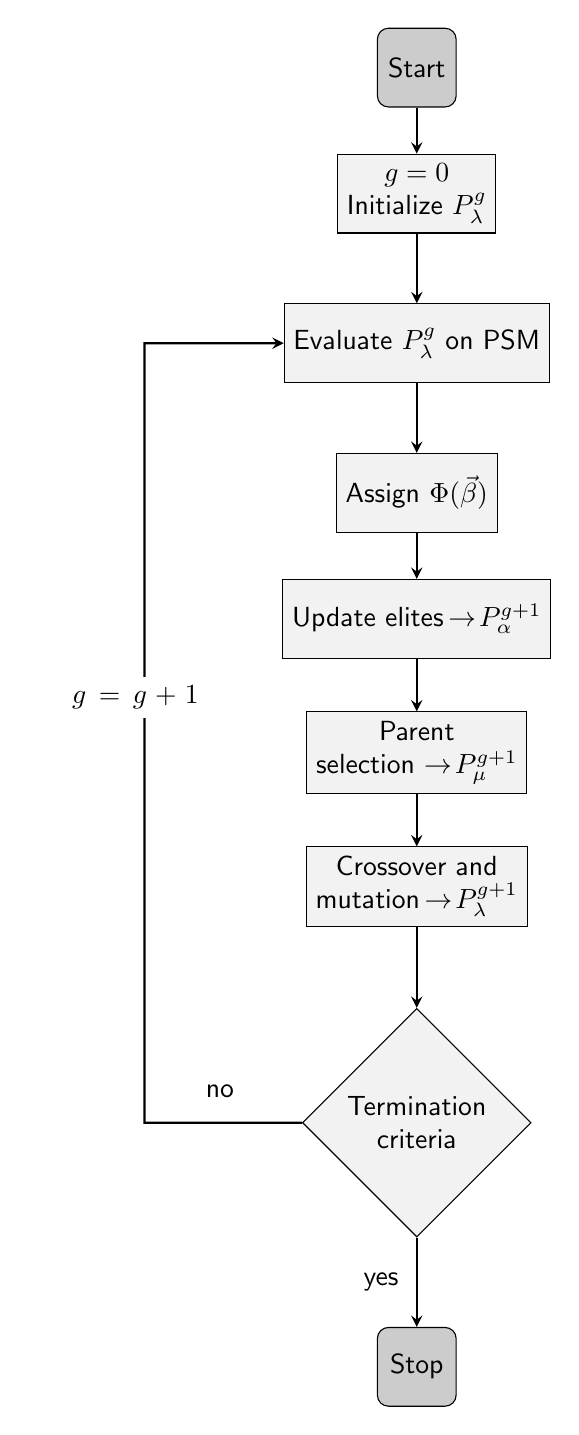
\begin{tikzpicture}[node distance=1.6cm,
    every node/.style={fill=white, font=\sffamily}, 
    align=center]
    
\node (start) [startstop] {Start};

\node (pro1) [process, below of=start] 
{ $g = 0$ \\ Initialize $P_{λ}^{g}$};

\node (pro2) [process, below of=pro1, yshift=-0.3cm] 
{Evaluate $P_{λ}^{g}$ on PSM};

\node (pro3) [process, below of=pro2, yshift=-0.3cm] 
{Assign $Φ(\vec{β})$};

\node (pro4) [process, below of=pro3] 
{Update elites $\!\rightarrow \!P_{α}^{g+1}$};

\node (pro5) [process, below of=pro4, yshift=-0.1cm]
{Parent \\ selection $\rightarrow \!P_{μ}^{g+1}$};

\node (pro6) [process, below of=pro5, yshift=-0.1cm] 
{Crossover and  \\
mutation $\!\rightarrow \!P_{λ}^{g+1}$};
 
\node (dec1) [decision, below of=pro6, yshift=-1.4cm] 
{Termination \\ criteria};
\node (stop) [startstop, below of=dec1, yshift=-1.5cm]
{Stop};

\draw [arrow] (start) -- (pro1);
\draw [arrow] (pro1) -- (pro2);
\draw [arrow] (pro2) -- (pro3);
\draw [arrow] (pro3) -- (pro4);
\draw [arrow] (pro4) -- (pro5);
\draw [arrow] (pro5) -- (pro6);
\draw [arrow] (pro6) -- (dec1);
\draw [arrow] (dec1) -- node[anchor=east, xshift=-0.1cm] 
{yes} (stop);
\draw [->][arrow] (dec1.west) -- ++(-2,0) -- ++(0,5.9) 
-- ++(0,4) -- node[xshift=-1cm,yshift=-4.5cm, text 
width=2.5cm]{$g = g +1 $}(pro2.west);
\draw (-2.5,-12.8) node[anchor=north]{no};

\end{tikzpicture}
\end{adjustbox}
\end{center}
\caption{Flowchart of Evolutionary Algorithms}
\label{fig:flowchart_EAs}
\end{figure}
\newpage
%-------------------------------------------------------

Most optimization problems are usually subject to 
constraints, which EAs handle via one of the following ways 
or a combination of those:

\begin{enumerate}
\item Penalty functions
\item Conversion of constraints into objectives
\item Correlation operators
\end{enumerate}

EASY in particular, mainly uses the first method, 
which penalizes any value that exceeds a certain threshold. 
That upper bound of acceptable constraint values is called 
nominal threshold value $c_{j}^{thres}$ and is firstly 
introduced in equation \ref{initial_opt_eq}. Once a constraint 
exceeds this value ($ c_{j}(\vec{β}) > c_{j}^{thres}$), an 
exponential penalty function $f_{l}(\vec{β})$ is triggered for each 
objective function $l \!\in \![1,n]$:
\begin{equation}\label{relaxation_function}
f_{n}(\vec{β}) = f_{n}(\vec{β}) + \prod_{j=1}^{n_{c}} exp
\left( α_{j} \dfrac{c_{j} - c_{j}^{thres}}
{c_{j}^{relax} - c_{j}^{thres}} \right)
\end{equation} 
\\
where $n$ and $n_{c}$ is the number of optimization 
objectives and constraints respectively, $α_{j}$ a 
user-defined positive constant and $c_{j}^{relax}$ a 
user-defined constraint value that is called relaxation 
threshold value. It is by definition larger than the nominal 
threshold value $c_{j}^{relax} > c_{j}^{thres}$ and is 
introduced in order to prompt the evolution process from 
terminating in its early stages, when the candidate solutions 
commonly defy the imposed constraints. When a candidate 
solution exceeds the relaxation threshold its fitness function 
$Φ(\vec{β})$ receives a death penalty i.e. an almost infinitely 
large value that practically renders the solution unsuitable 
for further evolution. Equation \ref{relaxation_function} 
operates when the candidate solutions reside in the $c_{j}^{thres} 
\!< \! c_{j} < c_{j}^{relax}$ range and penalizes them depending on 
their distance from the nominal threshold value $c_{j}^{thres}$ 
(see figure \ref{fig:feasible_sol}). Nominal threshold determines, 
therefore, which solutions are feasible and which are not.

\begin{figure}[h!]
\centering
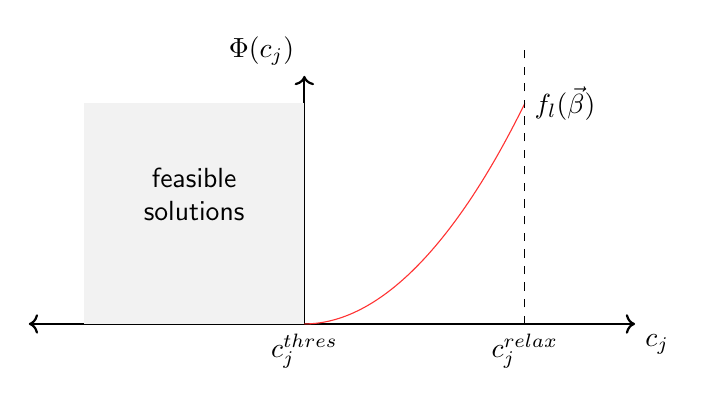
\begin{tikzpicture}[scale=0.7, every 
node/.style={font=\sffamily}, align=center]
\draw[thick,<->] (-5,0) -- (6,0) node[anchor=north west] 
{$c_{j}$};
\draw[thick,->] (0,0) -- (0,4.5) node[anchor=south east] 
{$Φ(c_{j})$};
\draw (0,0) [color=red!80] parabola (4,4); 
\draw (0,0) node[anchor=north]{$c_{j}^{thres}$};
\draw[dashed] (4,0) -- (4,5);
\draw (4,0) node[anchor=north]{$c_{j}^{relax}$}; 
\fill[color=gray!10] (0,0) rectangle (-4,4); 
\draw (-2,3) node[rotate=0, anchor=north]
{feasible \\ solutions};
\draw (4,4) node[anchor=west]{$f_{l}(\vec{β})$};
\end{tikzpicture}
\caption{Penalisation of feasible and infeasible 
solutions in EASY}
\label{fig:feasible_sol}
\end{figure} 

\newpage
%------------------------------------------------------
%-------------------------------------------------------

\chapter{MAEAs with off-line training}
Off-line trained surrogate models are built prior to the 
evolution and are trained primarily on a dataset of training 
patterns, which cover the entirety of the design space and are 
collected via the implementation of various DoE techniques. The 
training process is disconnected from the evolution and, thus, this 
method is described as static. MAEAs with off-line training can be 
decomposed in the following steps:

\begin{OFFL}
\item \textbf{Design of Experiments (DoE)} \\
One of the various DoE techniques is applied and the sampling 
process initiates, which involves the selection of $n_{doe}$ 
observations $\vec{χ} \! \in \! \mathbb{R}^{n_{β}}$ from within 
the imposed bounds of the design space. Subsequently, the necessary 
objective function values $\vec{f}(\vec{χ})$ are computed on the 
PSM. Consequently, the resulting $n_{doe}$ $(\vec{χ},\vec{f}
(\vec{χ}))$ observed pairs are archived in a database reserved for 
the training of the metamodels which is referred to as metamodel 
database (MDB). Any untried point in the design space that is not 
archived in the MDB, i.e. each candidate solution, is denoted by 
$\vec{β} \in \mathbb{R}^{n_{β}}$.

\item \textbf{Training of the metamodel}\\
The $n_{t}$ archived $(\vec{χ},\vec{f}(\vec{χ}))$ pairs  are used 
in the training of the metamodel. In the first optimization cycle, 
the number of training patterns $n_{t}$ is equal to the $n_{doe}$ 
observations. DoE techniques are applied mainly in MAEAs with 
off-line training and are used to collect training patterns from 
the entirety of the design space, resulting in the construction of 
a global metamodel. 

\item \textbf{Implementation of EAs}\\
The optimization process initiates subsequently via the
use of the EASY software that implements EAs. The evolution 
follows the process described in section \ref{section:EAs} 
with one main variation; the offspring evaluation in step 2 
(EAs-2) is performed via the use of the trained surrogate 
model. The metamodel serves as a black box that approximates $λ$ 
individuals, where $λ$ is the number of offspring in the 
$P_{λ}^{g}$ set, and provides the corresponding prediction of 
the objective function value \scalebox{0.86}{%
$\hat{\vec{f}}(\vec{β})$}, $\forall \vec{β} \!\in \!P_{λ}^g$. Each 
prediction \scalebox{0.86}{%
$\hat{\vec{f}}(\vec{β})$ } is assigned a scalar fitness function 
value $\hat{Φ}(\vec{β})$, which in MOO problems is based on 
dominance criteria and $\hat{Φ}(\vec{β}) \!\equiv \!\hat{f}
(\vec{β})$ in SOO. The criterion that prohibits EAs from exceeding 
a selected number of evaluations is accordingly modified to fit the 
trivial computational cost of the metamodel.  

\newpage
%----------------------------------------------------------------

%\begin{figure}[h]
%\centering
%\begin{tikzpicture}[scale=0.6, every 
%node/.style={font=\sffamily}, align=center]
%\draw[thick,->, color=blue!70] (-7,2) -- (-5,2) 
%node[anchor=south east, xshift = -0.4 cm, color = black!100] 
%{$\vec{β}$}; 
%\filldraw [color=gray!40] (0,0) rectangle (-4,4);
%\draw (-2,3) node[rotate=0, anchor=north]{SMT \\ source code};
%\draw[thick,->, color=blue!70] (1,2) -- (3,2) 
%node[anchor=south east, xshift = -0.2 cm, color = black!100] 
%{$\hat{f}(\vec{β})$};
%\draw [red,thick,dashed] (-10,-0.75) rectangle (6.5,5) 
%node[anchor=north east]{step EAs-3};
%\end{tikzpicture}
%\caption{Use of metamodel as a black box}
%\end{figure}

\item \textbf{Re-evaluation on the PSM}\\
The re-evaluation process initiates once the evolution 
has been completed and the optimal candidate solutions have 
been found. The best candidate solution in SOO or a set of 
$λ_{α}^{(i)}$ non-dominated solutions in MOO, residing in the 
$P_{e}^{(i)}$ temporary set, are re-evaluated using the exact PSM. 
Index \textit{i} is used to denote the current cycle of the MAEA 
algorithm using off-line training. 

\item \textbf{Termination}\\
The deviation between the metamodel and the PSM evaluated 
objective function values determines the convergence of the 
MAEA-based optimization. In case the convergence criteria are not 
met, the optimal candidate solution/s residing in 
the $P_{e}^{(i)}$ set at the end of the evolution or some others 
arbitrarily selected individuals are used to update the 
existing MDB. The outcome of their evaluation, i.e. 
$\vec{f}(\vec{β})$, $\forall \vec{β} \!\in \!P_{e}^{(i)}$, is 
subsequently added to the updated MDB and the $i_{th}$ evolution 
terminates. The next cycle of the optimization initiates 
starting from step 1 (OFFL-1) and index \textit{i} is set to 
$i \leftarrow i+1$. The evolution's inability to yield an 
optimal solution is indicative of a poorly trained surrogate 
model and, therefore, an improved metamodel needs to be 
trained. Consequently in step 1 (OFFL-1) of the $(i+1)_{th}$ 
cycle, DoE techniques are implemented to select $n_{new\_doe}$ 
new points and in the following step (OFFL-2) a new metamodel 
is built on $n_{t}$ training patterns, where:
\begin{equation}\label{off_line_nt}
n_{t} = n_{doe} + \sum_{i=0}^{i} \left( λ_{α}^{(i)} +
n_{new\_doe} \right) 
\end{equation}
\\[-0.1cm]
where $λ_{α}^{(i)}$ is the number of elites selected in the 
$i_{th}$ generation and $n_{new\_doe}$ a user-defined number of 
sample points that is sampled via DoE techniques at the start 
of each optimization cycle in order to fill the MDB and improve 
the fitting of the metamodel. The updated number of sample points 
will be denoted by $n_{doe}^{'}$ for simplicity, where:
\begin{equation}
n_{doe}^{'} = n_{doe} + \sum_{i=0}^{i} \left(n_{new\_doe} \right)
\end{equation} 

The aforementioned steps outline the function of MAEAs with 
off-line trained metamodels and will be subsequently combined into 
the flowchart form of figure \ref{fig:offline_flowchart}.
\end{OFFL} 

\newpage
%--------------------------------------------------------


\begin{figure}[h!]
\centering
\begin{adjustbox}{width=0.9\textwidth,height= 
1\textheight,keepaspectratio}
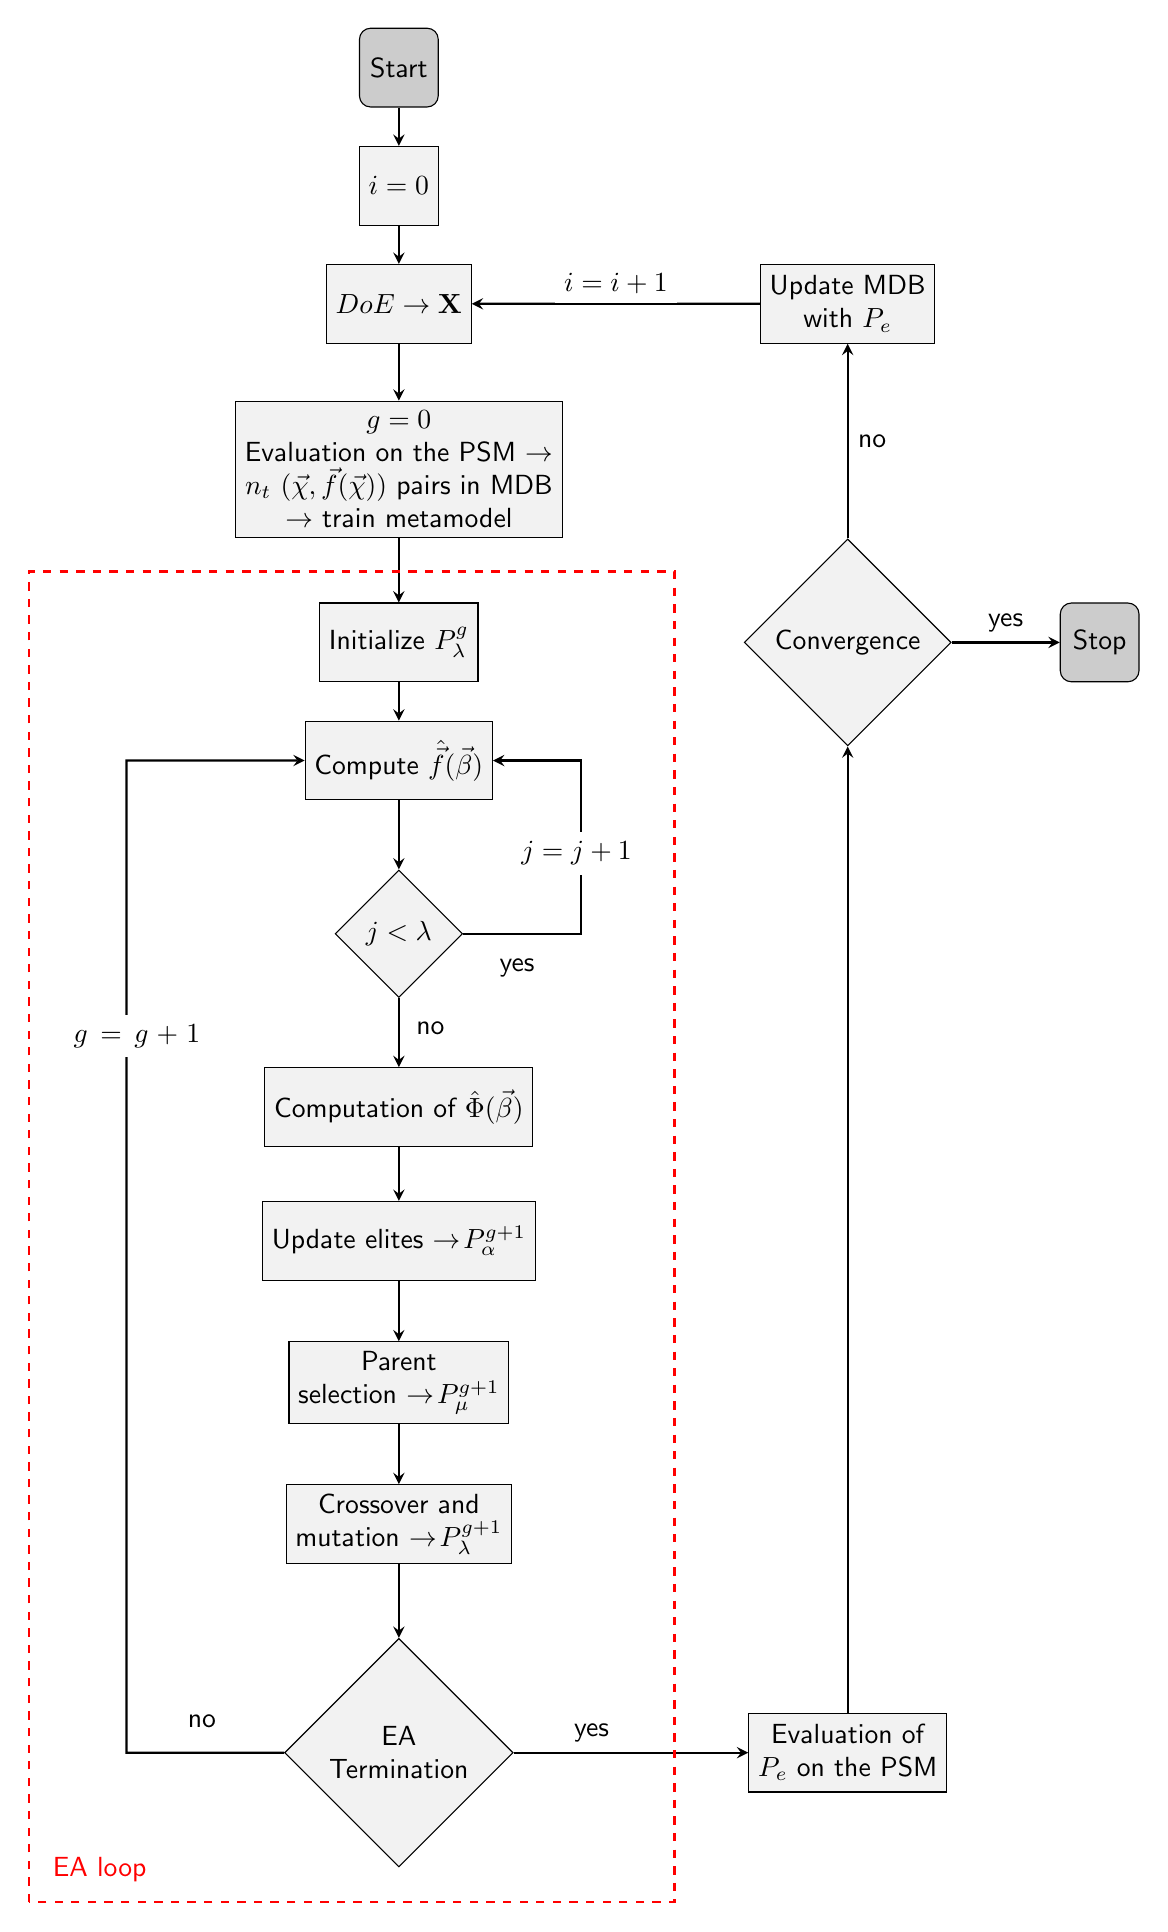
\begin{tikzpicture}[node distance=1.7cm,
    every node/.style={fill=white, font=\sffamily}, 
    align=center]
\node (start) [startstop] {Start};
\node (pro0) [process, below of=start, yshift=0.2cm] 
{$i = 0$};

\node (pro1) [process, below of=pro0, yshift=0.2cm] 
{$DoE \rightarrow \mathbf{X}$};

\node (pro2) [process, below of=pro1, yshift=-0.4cm] 
{$g=0$ \\ Evaluation on the PSM $\rightarrow$
\\ $ n_{t}$ $(\vec{χ}, \vec{f}(\vec{χ}))$ pairs in MDB \\
$\rightarrow$ train metamodel};

%------------------EA loop--------------------------------
\node (init1) [process, below of=pro2, yshift=-0.5cm] 
{Initialize $P_{λ}^{g}$};

\node (pro3) [process, below of=init1, yshift=0.2cm] 
{Compute $\hat{\vec{f}}(\vec{β})$};

\node (dec3) [decision, below of=pro3, yshift=-0.5cm] 
{$j < λ$};

\node (pro4) [process, below of=dec3, yshift =-0.5cm] 
{Computation of $\hat{Φ}(\vec{β})$};

\node (pro5) [process, below of=pro4] 
{Update elites $\rightarrow \!P_{α}^{g+1}$};

\node (pro6) [process, below of=pro5, yshift=-0.1cm]
{Parent \\ selection $\rightarrow \!P_{μ}^{g+1}$};

\node (pro7) [process, below of=pro6, yshift=-0.1cm] 
{Crossover and \\ mutation $\rightarrow \!P_{λ}^{g+1}$};

\node (dec1) [decision, below of=pro7, yshift=-1.2cm] 
{EA \\ Termination};
%-------------------------------------------------------------

\node (pro8) [process, right of=dec1, xshift=4cm] {Evaluation of \\ 
$P_{e}$ on the PSM};

\node (dec2) [decision, right of=init1, xshift=4cm] 
{Convergence};

\node (pro9) [process, above of=dec2, yshift = 2.6cm] 
{Update MDB \\ with $P_{e}$};

\node (stop) [startstop, right of=dec2, xshift=1.5cm]
{Stop};

\draw [arrow] (start) -- (pro0);
\draw [arrow] (pro0) -- (pro1);
\draw [arrow] (pro1) -- (pro2);
\draw [arrow] (pro2) -- (init1);
\draw [arrow] (init1) -- (pro3);
\draw [arrow] (pro3) -- (dec3);
\draw [arrow] (dec3) -- (pro4);
\draw [arrow] (pro4) -- (pro5);
\draw [arrow] (pro5) -- (pro6);
\draw [arrow] (pro6) -- (pro7);
\draw [arrow] (pro7) -- (dec1);
\draw [arrow] (pro8) -- (dec2);

%-----------arrow dec1------------------
\draw [arrow] (dec1.east) -- node[anchor=south, 
xshift = -0.5cm] {yes}(pro8.west);
\draw [->][arrow] (dec1.west) -- ++(-2,0) -- ++(0,12.6) 
-- ++(2,0) -- node[xshift=-2cm,yshift=-3.5cm, text 
width=2.5cm]{$g = g +1 $}(pro3.west);

%-----------arrow dec2-------------------
\draw [arrow] (dec2.north) -- node[anchor=west]{no} 
(pro9);
\draw [arrow] (dec2) -- node[anchor=south]{yes}(stop);
\draw (-2.5,-20.8) node[anchor=north]{no};

%------------draw rectangle--------------
\draw [red, thick, dashed] (-4.7,-23.3) rectangle 
+(8.2,16.9);
\draw [red] (-3.8,-22.6) node[anchor=north]{EA loop};

%------------draw pro9-------------------
\draw [arrow] (pro9) -- node[anchor=south]{$i=i+1$}(pro1);

%-----------arrow dec3-------------------
\draw [arrow] (dec3.east) -- ++(1.5,0) -- ++(0,2.2) 
-- ++(-1,0) -- node[anchor=north, xshift = 1cm, 
yshift=-0.9cm] {$j=j+1$}(pro3.east);
\draw (0.4,-12) node[anchor=north]{no};
\draw (1.5,-11.2) node[anchor=north]{yes};


\end{tikzpicture}
\end{adjustbox}
\caption{Flowchart of MAEAs using off-line trained 
metamodels}
\label{fig:offline_flowchart}
\end{figure}

\newpage
%--------------------------------------------------------


\section{Design of Experiments (DoE)}
The predominant characteristic of off-line trained MAEAs is the 
construction of a single global surrogate model 
\cite{global_metamodel}. The majority of necessary patterns 
for the training of this global metamodel are collected via the 
use of various Design of Experiments (DoE) techniques that sample 
the entirety of the design space. DoE is a statistical tool used 
for analyzing the interactions between the parameters that 
effect the performance of a system and controlling them 
in order to optimize its performance\cite{DOE,DOE1,DOE2}.
%In metamodel construction, DoE techniques are implemented 
%to map the response $\vec{f}(\vec{χ}) \!\in \!\mathbb{R}^{n}$ to 
%each observation $\vec{χ}$. 
The most commonly used DoE techniques and the ones studied in this 
thesis are the following: 

\begin{enumerate}
\item \textbf{Random sampling} \\
The most common technique of removing bias from a design is 
randomization, which gives each sample point $\vec{χ} \!= \! 
[χ_{1}, χ_{2}, \hdots, χ_{n_{β}}] \in \mathbb{R}^{n_{β}}$ 
equal probability of being selected from the design 
space \cite{Random}, as shown in figure \ref{fig:random}. 

\vspace{-4mm}
  
\begin{figure}[h!]
    \centering
    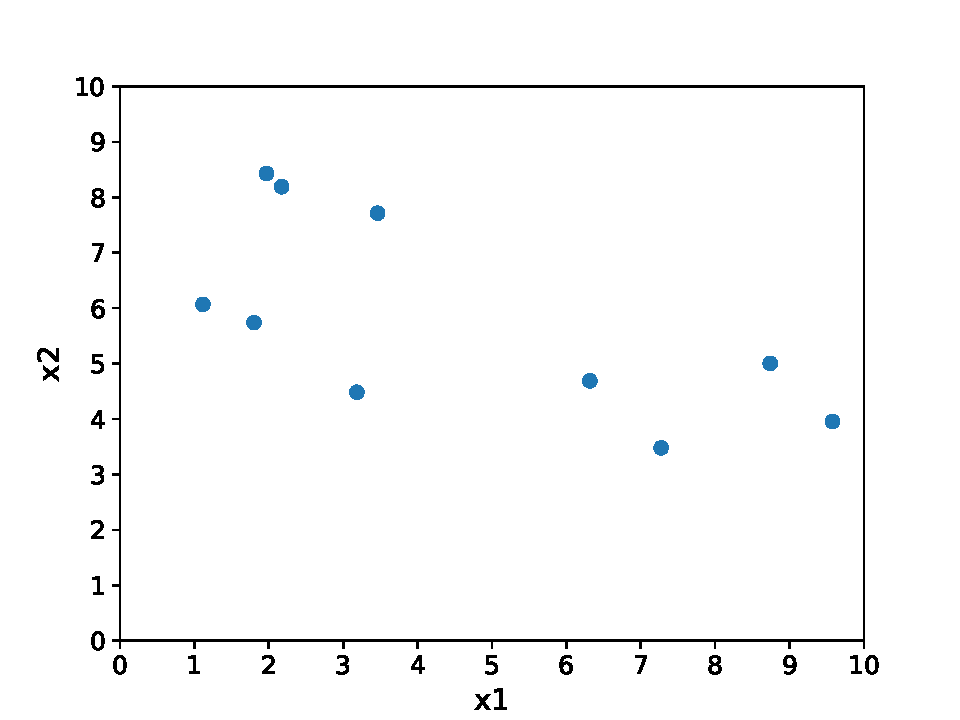
\includegraphics[width=0.47\textwidth]{random_SMT.pdf} 
    \caption{Random design in 2D space for $n_{doe} \!= \!10$ 
    sample points}
    \label{fig:random}   
\end{figure}

\item \textbf{Latin Hypercube Sampling (LHS)}  \\ 
A square grid containing a single sample point $\vec{χ} \in 
\mathbb{R}^{2}$ per row and column is called a Latin Square.
The generalization of this design in $n_{β} \!> \!2$ dimensions 
results in the creation of a Latin Hypercube (LH)\cite{Latin 
Hypercube}. A Latin Hypercube Design (LHD) aims to improve the 
coverage of the design space and eliminate the probability of two 
coinciding sample points and is created via the implementation of 
LHS\cite{LHS, LHS method} scheme. In LHDs, the design space in 
each dimension is stratified into $n_{doe}$\footnote{The original 
design ($i=0$) consists of $n_{t} = n_{doe}$ points, while a 
separate design is constructed for every $n_{new\_doe}$ points 
sampled. Without loss of generality, we assume from this point 
forward that in the description of DoE we refer to the original 
design of $n_{doe}$ points.} equiprobable and non-overlapping 
intervals\cite{LHS}, called strata. Subsequently, $n_{doe}$ 
distinct values are selected, one from each stratum, and are 
paired to form the components $χ_{1}, χ_{2}, \hdots, χ_{n_{β}}$ of 
each sample vector $\vec{χ} \!\in \!\mathbb{R}^{n_{β}}$. As a 
result of the stratification, the LHD consists of $n_{doe}$ 
distinct sample points and can be written as a $n_{doe} \times 
n_{β}$ matrix $\mathbf{X} = [\vec{χ}_{1}, \vec{χ}_{2}, \hdots, 
\vec{χ}_{n_{doe}}]^T$, where each component $\vec{χ}_{i} = [χ_{i,
1}, χ_{i,2},\hdots, χ_{i,n_{β}}]$ represents an observation 
$\vec{χ} \in \mathbb{R}^{n_{β}}$. LHDs can be enhanced with 
several optimality construction criteria, some of which are 
presented here \cite{preprint_SMT,pyDOE}:

\newpage
%-----------------------------------------------------------


\begin{enumerate}
\item \textbf{Centered LHD} \\
This construction criterion centers the selected values from within 
each hypercube, as shown in figure \ref{fig:centered_LHD}. 

\vspace{-2mm}

\begin{figure}[h!]
    \centering
    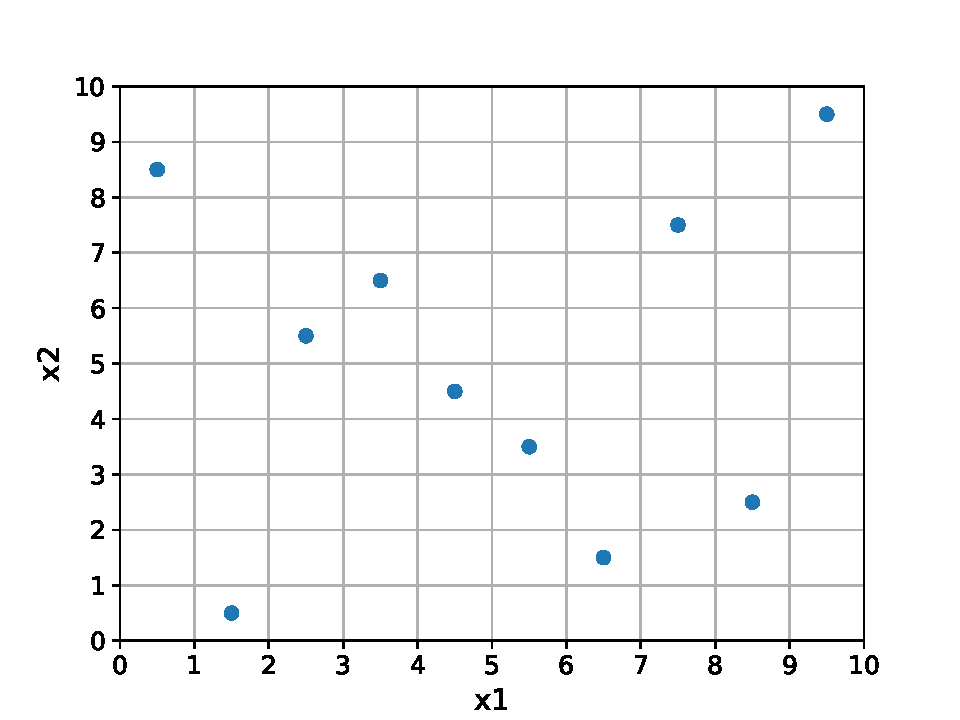
\includegraphics[width=0.5\textwidth]{criterion_c.pdf}    
    \caption{Centered LHD in 2D space. The grid has been modified 
    to facilitate the visualization of $n_{doe} = 10$ strata in 
    each dimension.}
    \label{fig:centered_LHD}
\end{figure}
    
\item \textbf{Maximin LHD} \\
This construction criterion was introduced by Johnson et al.
\cite{maximin} based on the idea that the Euclidean distance 
between sample points should be used as a metric for design 
construction. A maximin design, denoted by $S_{Mm}$, 
guarantees that every pair of points will never coincide by 
maximizing the minimum distance between them \cite{maximin2}.
\begin{equation}\label{maximin}
\max\limits_{S \subset \mathbb{R}^{n_{β}}} 
\min\limits_{\vec{χ}_{i}, \vec{χ}_{j} \in S} d(\vec{χ}_{i}, 
\vec{χ}_{j} ) = 
\min\limits_{\vec{χ}_{i}, \vec{χ}_{j} \in S_{Mm}} 
d(\vec{χ}_{i}, \vec{χ}_{j}) 
\hspace{3mm} ,\forall i,j \in [1,n_{doe}]
\end{equation}

Each selected point $\vec{χ} \!\in \!S$, where $S$ the selected 
design set, is the center of a sphere, the radius of which is 
calculated by the algorithm that produces the maximin design 
described by eq. \ref{maximin}. Consequently, the final design 
contains $n_{doe}$ non-overlapping spheres. In a maximin LHD, the 
sample points must furthermore be selected from within within each 
hypercube, as shown in figure \ref{fig:maximin_LHD}.

\vspace{-2mm}

\begin{figure}[h!]
    \centering
    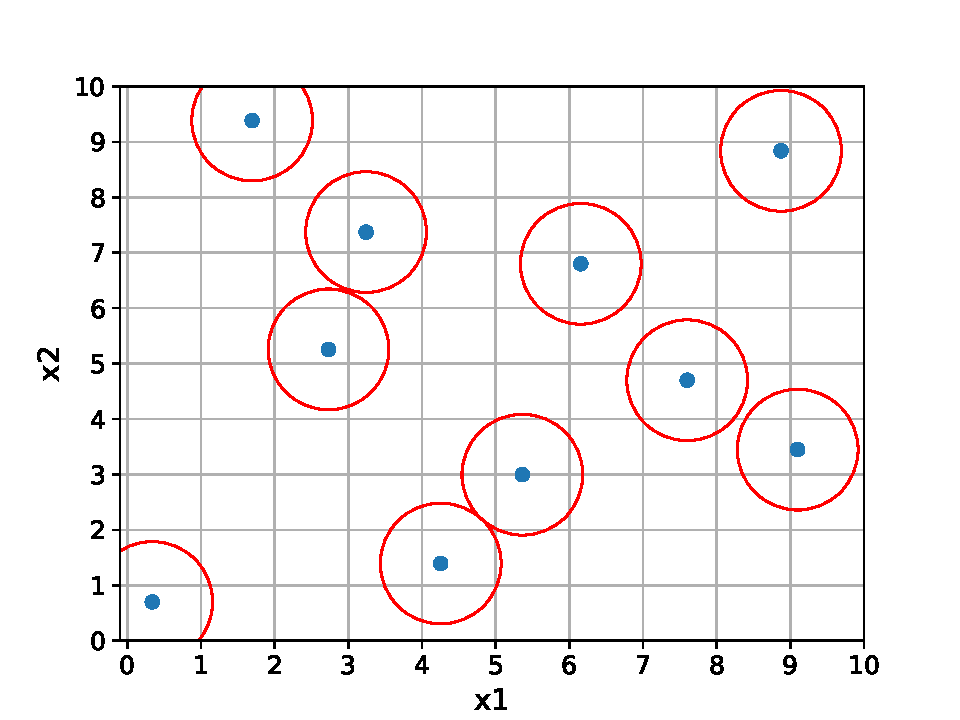
\includegraphics[width=0.5\textwidth]{criterion_m.pdf}    
    \caption{Maximin LHD in 2D space for $n_{doe} = 10$ 
    sample points}
    \label{fig:maximin_LHD}
\end{figure}

\newpage
%--------------------------------------------------------------


\item \textbf{Maximin Centered LHD} \\
Similar to maximin LHD with the exception that the selected sample 
points are centered within each hypercube, as shown in figure 
\ref{fig:maximin_centered_LHD}.

\vspace{-4mm}

\begin{figure}[h!]
    \centering
    \includegraphics[width=0.47\textwidth]{criterion_cm.pdf}    
    \caption{Maximin centered LHD in 2D space for $n_{doe} = 10$ 
    sample points}
    \label{fig:maximin_centered_LHD}
\end{figure}

\item \textbf{Maxent LHD} \\
Information entropy as proposed by Shannon \cite{entropy} is 
directly associated to the level of information available from a 
design. Shewry and Wynn \cite{max_entropy} showed that maximizing 
the entropy of the response distribution at the sampled design 
sites $\mathbf{X}$ is equivalent to maximizing the gain of 
information of the response distribution at any untried location of 
the design space. If the response distribution is given by a 
stationary Gaussian process $Y(\cdot)$ with mean $μ_{Y}$, 
variance $σ^{2}$ and correlation function $R(\cdot)$, then the 
optimal design $S \!\subset \!\mathbb{R}^{n_{β}}$ can be found by 
maximizing the simplified entropy of the distribution of the 
responses at the design sites, as such:  
\begin{equation}
\max\limits_{\vec{χ}_{i}, \vec{χ}_{j} \in S} - 
ln\left[det\mathbf{R}(\vec{χ}_{i}, \vec{χ}_{j})\right]
\end{equation}
\\[-2mm]
where $\mathbf{R}(\vec{χ}_{i}, \vec{χ}_{j}) = \prod_{l=1}^{n_{χ}}
exp( -\theta_{l} \left| χ_{i,l} - χ_{j,l} \right|^{q})$ and $q$ a 
positive integer with values 1 or 2, corresponding to an 
exponential or a Gaussian kernel, respectively. The parameters 
$θ_{l}$ denote the degree of correlation between training points 
w.r.t. each design dimension $l \!\in \![1,n_{β}]$. In a maxent 
LHD, the sample points must furthermore be selected from within 
within each hypercube, as shown in figure \ref{fig:maxent_LHD}.

\vspace{-4mm}

\begin{figure}[h!]
    \centering
    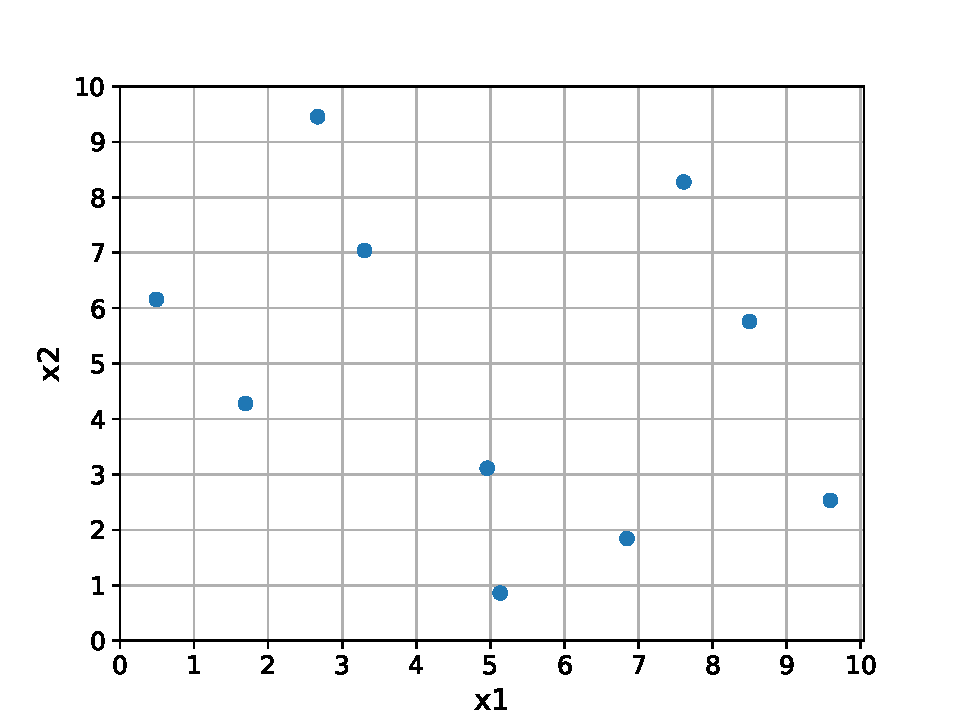
\includegraphics[width=0.47\textwidth]{criterion_corr.pdf}    
    \caption{Entropy LHD in 2D space for $n_{doe} = 10$ 
    sample points}
    \label{fig:maxent_LHD}
\end{figure}

\newpage
%--------------------------------------------------------------


\item \textbf{Enhanced Stochastic Evolutionary (ESE) LHD} \\
This criterion is an enhancement to the existing global 
search, stochastic evolutionary (SE) algorithm, originally 
developed by Saab and Rao\cite{SE}. The need to further 
reduce the computational cost of SE resulted in the creation 
of Enhanced Stochastic Evolutionary algorithm (ESE
)\cite{ESE}. This new approach is based on utilizing 
efficient methods for evaluating various space-filling criteria, 
namely $φ_{p}$, entropy and centered $L_{2}$ discrepancy 
criterion. The first criterion was proposed by Morris and Mitchel 
(1995)\cite{fp criterion} and is an extension of the maximin 
criterion. $L_{2}$ discrepancy is the most common expression of 
$L_{p}$ discrepancy, which is a metric of non-uniformity of a DoE. 
The formula used to describe centered $L_{2}$ or $CL_{2}$ 
discrepancy was proposed by Hickernell (1998)\cite{discrepancy}. 
The minimization of $CL_{2}$ discrepancy results in a uniform 
design. ESE combines these three aforementioned space-filling
criteria to construct an optimal design. In a ESE LHD, the sample 
points must furthermore be selected from within within each 
hypercube, as shown in figure \ref{fig:ESE_LHD}.

\begin{figure}[h!]
    \centering
    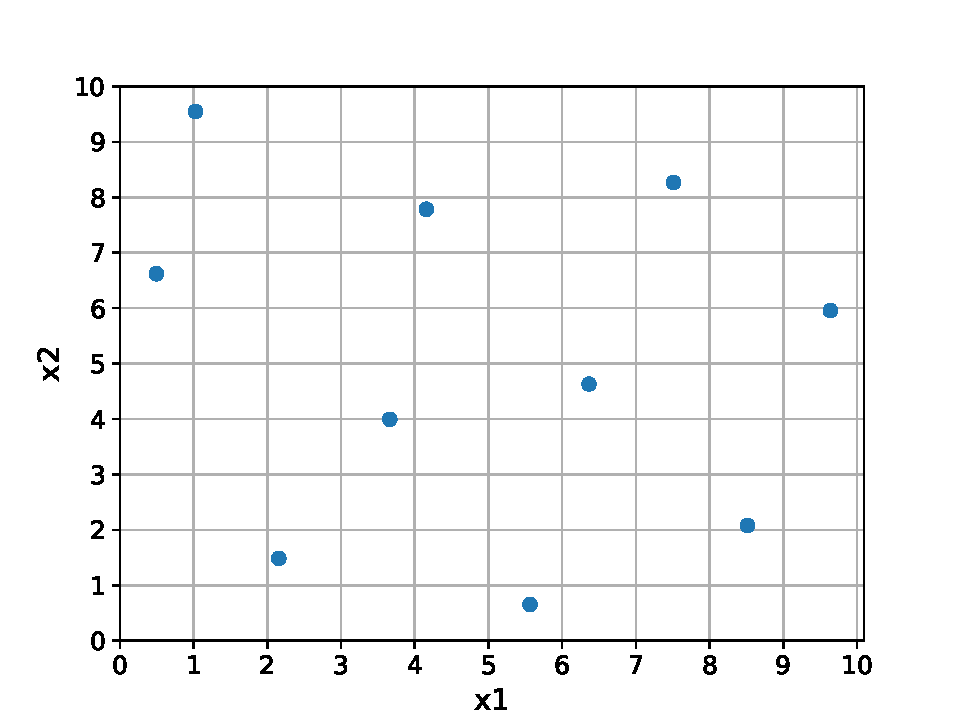
\includegraphics[width=0.5\textwidth]{criterion_ese.pdf}    
    \caption{ESE LHD in 2D space for $n_{doe} = 10$ 
    sample points}
    \label{fig:ESE_LHD}
\end{figure}

\end{enumerate}

The quality of the LHD affects the convergence of the 
MAEA-based optimization process and therefore selecting the 
most cost-efficient construction criterion of an LHD is essential 
for the success of this method. An analysis performed in appendix 
\ref{appendix:constr_crit}, concluded that ESE LHDs are the most 
suitable for the purpose of this thesis and therefore the LHS 
scheme is modified accordingly to produce such designs.

\newpage
%--------------------------------------------------------


\item  \textbf{Factorial sampling}\\
In a factorial design, the relative importance of each design 
variable (factor) on the objective function is tested by 
replicating all the possible combinations of the factors. 
Each possible combination is replicated in a run of the 
design with a total of $n_{doe}$ runs being performed. Each 
factor is assigned a number of discrete values in the [-1,1] 
range, called levels, where high and low influence are 
assigned a level of 1 and -1 respectively\cite{Factorial}. 
The change in response caused by an alteration in the level 
of each factor can, therefore, be correlated with the 
relative importance of each factor. The complete replicate 
of a factorial design that contains all possible combinations 
between $n_{β}$ factors is called a Full Factorial Design 
(FFD). A conventional FFD is performed at 2 levels, i.e 1 
and -1, which results in $n_{doe} = 2^{n_{β}}$ possible 
combinations\cite{Full_Factorial2}. However, the number of 
factorial runs $n_{doe}$ is user-defined, i.e. 
$n_{doe} \! \neq \! 2^{n_{β}}$ or $n_{doe} \neq 3^{n_{β}}$, 
and the cost of constructing a FFD grows exponentially 
as the number of factors increases. In order to overcome the 
imposed restrictions, interactions between factors that yield
the lowest response are neglected. The resulting design is a  
fractional factorial design\cite{Fractional Factorial}; such a 
design is depicted in the following case for $n_{doe} = 10$
sample points in figure \ref{fig:Full_Fact_example}:

\begin{table}[h!]
\centering
\begin{tabular}{|c|c|c|c|c|c|}
\toprule
\rowcolor{gray!20} \textbf{Levels}
 & \textbf{-1} & \textbf{-0.5} & \textbf{0} 
 & \textbf{0.5} & \textbf{1} \\ 
\midrule
\textbf{$χ_{1}$} & 6 & 7.33 & - & 8.66 & 10 \\ 
\hline 
\textbf{$χ_{2}$} & 150 & - & 175 & - & 200 \\ 
\bottomrule
\end{tabular}
\end{table} 

\begin{figure}[h!]
    \centering 
    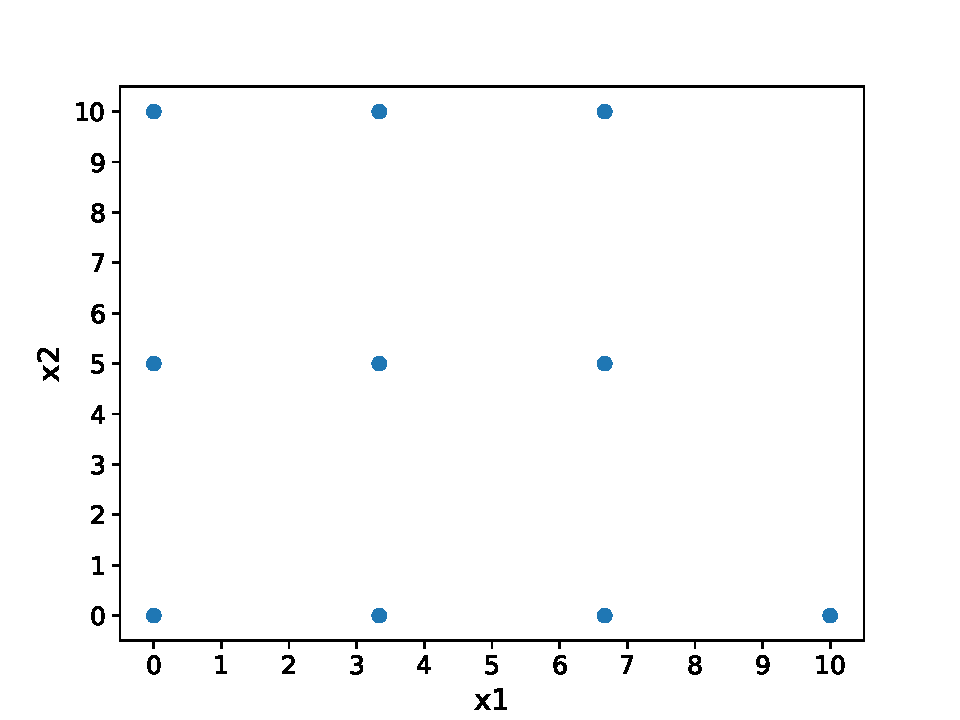
\includegraphics[width=0.5\textwidth]
    {full_factorial_SMT.pdf} 
    \caption{Example of Factorial design for 2 design 
    variables with $n_{doe} = 10$ sample points}
    \label{fig:Full_Fact_example}
\end{figure} 

\end{enumerate}

\newpage
%-------------------------------------------------------


\subsection{Comparison between DoE construction schemes}
The selection of a suitable design is an essential step to
the training of a surrogate model. For that reason the 
available DoE construction schemes are evaluated w.r.t. their
effect on the training process of the metamodel. The 
comparison is limited to Factorial and LH designs, since they 
tend to be the most reliable in overall coverage of the design 
space and especially in the selection of a representative sample 
from the total population set. Random designs are eliminated from 
the assessment process, since they are considered unfit for large 
population sets due to equiprobable selection of each individual. 
Optimality space-filling criteria are not utilized in random 
designs and the outcome is a design that either contains a number 
of similar sample points or omits significant sample points 
that are of great importance to the training of the 
surrogate model \cite{Random}.

The first difference between the two remaining DoE 
construction schemes is detected in the selection process of 
sample points. In both full and fractional factorial designs, the 
sample points are distributed as evenly as possible in the 
$n_{β}$-dimensional design space, utilizing its full 
capacity. In LHDs, the design space is stratified and the 
sample points are selected from within the created intervals 
via the use of some space-filling construction criterion. 
For up to $n_{β} = 3$ design variables the resulting designs can 
be replicated in 3D space as depicted in figure 
\ref{fig:LH_vs_FD_in3D}; in this example the design space is 
created by the bounds of each design variable in eq. 
\ref{pseudo_aircraft}.

 \begin{figure}[h!]
    \centering
    \begin{subfigure}[b]{0.50\textwidth}
    \centering
    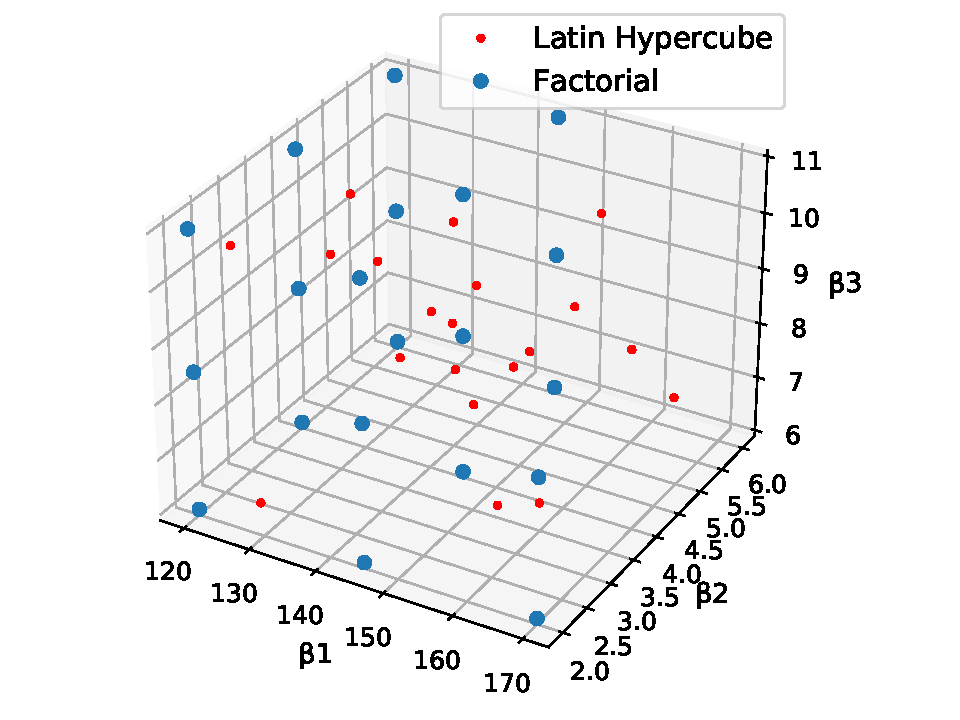
\includegraphics[width=\textwidth]{lhs_vs_fullf1.pdf}
    \caption{3D design space} 
    \end{subfigure}  
\hfill
\begin{subfigure}[b]{0.49\textwidth}
    \centering
    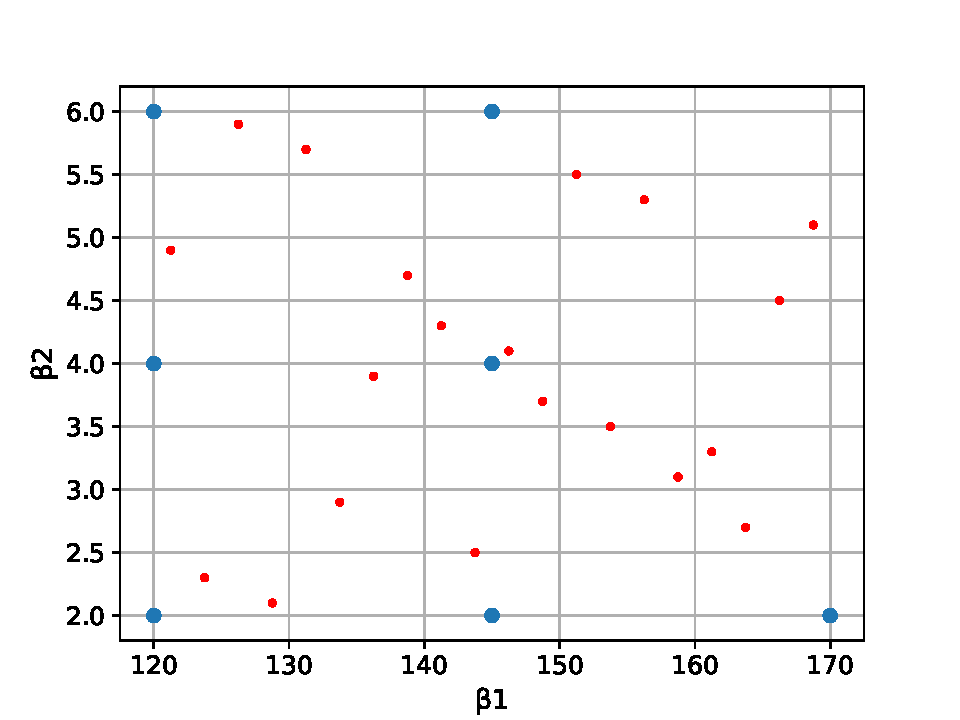
\includegraphics[width=\textwidth]{lhs_vs_fullf2.pdf} 
    \caption{2D contour surface along $χ_{1}$, $χ_{2}$ plane}
    \end{subfigure}
\hfill
\begin{subfigure}[b]{0.49\textwidth}
    \centering
    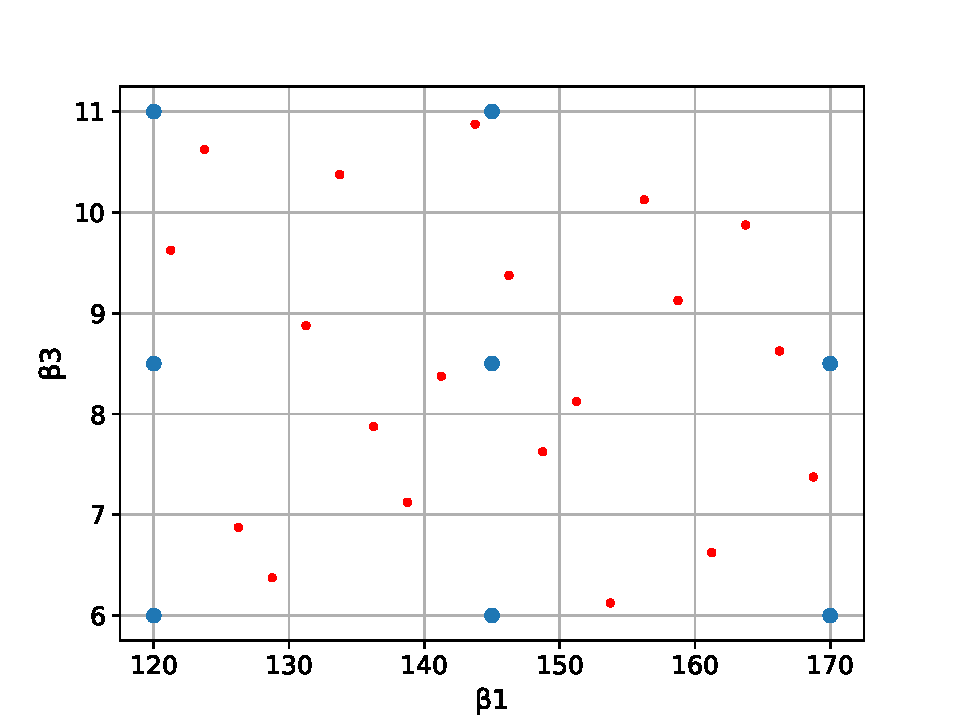
\includegraphics[width=\textwidth]{lhs_vs_fullf3.pdf} 
    \caption{2D contour surface along $χ_{1}$, $χ_{3}$ plane}
    \end{subfigure}
\hfill
\begin{subfigure}[b]{0.49\textwidth}
    \centering
    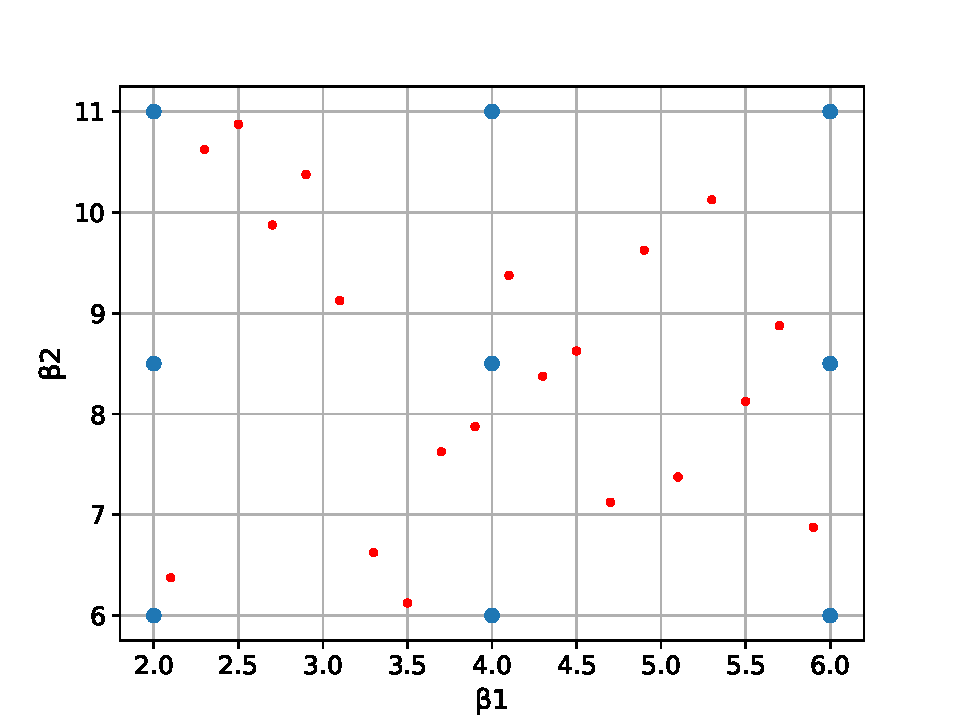
\includegraphics[width=\textwidth]{lhs_vs_fullf4.pdf}
    \caption{2D contour surface along $χ_{2}$, $χ_{3}$ plane} 
    \end{subfigure}
\caption{Factorial and LH designs in 3D design 
space} 
\label{fig:LH_vs_FD_in3D}      
\end{figure}

\newpage
%-----------------------------------------------------------


The implementation of factorial sampling in 3D space for 
$n_{doe} = 20$ runs results in the creation of a fractional 
factorial design, which disregards a large section of the design 
space. For the same number of runs, on the other hand, LHS scheme 
spreads sample points optimally across the design space and yields, 
for this reason, better designs. In LHDs furthermore, the MDB is 
more diverse and complete, since it consists of $n_{doe}$ distinct 
values, unlike in factorial designs where the influence of each 
design variable is tested on $κ_{l} < n_{doe}$ levels each. The 
responses of $n_{doe}$ sample points can be written as a $n_{doe} 
\times n$ matrix $\mathbf{F} = [\vec{f}_{1}, \vec{f}_{2}, \hdots, 
\vec{f}_{n_{doe}}]^{Τ}$, where each component $\vec{f}_{i} = 
[f_{i,1}, f_{i,2}, \hdots, f_{i,n}]$ represents a response $\vec{f} 
\in \mathbb{R}^{n}$. The responses of $n_{doe} = 20$ sample
points in eq. \ref{pseudo_aircraft} (see appendix chapter 
\ref{appendix:pseudo_aircraft}) are depicted in figure 
\ref{fig:Factorial_vs_LHS}.

\vspace{-3mm} 
\begin{figure}[h!]
    \centering
    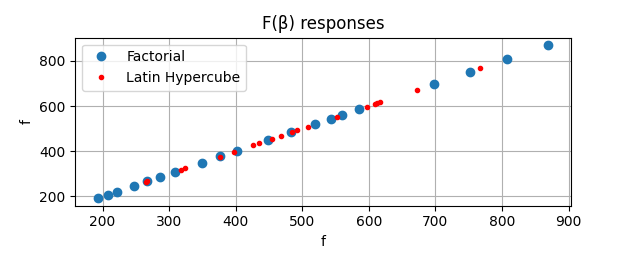
\includegraphics[width=0.6\textwidth]{Figure_31}   
    \caption{Comparison between $\mathbf{F}(\vec{χ})$ 
    responses to samples created via Factorial and LHS DoE scheme}
    \label{fig:Factorial_vs_LHS}
\end{figure}

The two DoE schemes yield similar objective function values, 
as seen in figure \ref{fig:Factorial_vs_LHS}). However, a 
similarity in objective function responses cannot lead to any 
definite conclusions on the quality of the respective models. One 
of many metrics for metamodel quality is the Root Mean Square 
Error (RMSE) (see appendix chapter \ref{appendix:constr_crit}). 
This metric depends on the order of magnitude of the observed 
values and the size of the sample, so it is merely used in the 
comparison of various metamodels when approximating the same PSM 
and trained on the same dataset.  Consequently, a high RMSE is a 
characteristic of a model that has been selectively trained for 
only a narrow set of sample points, therefore lacking in 
robustness. This concept is tested in a KPLS model with fitting  
shown in figure \ref{fig:LHD_FD_training}.

 \begin{figure}[h!]
    \centering
    \begin{subfigure}[b]{0.49\textwidth}
    \centering
    \caption{LHD, NRMSE = 0.003818}
    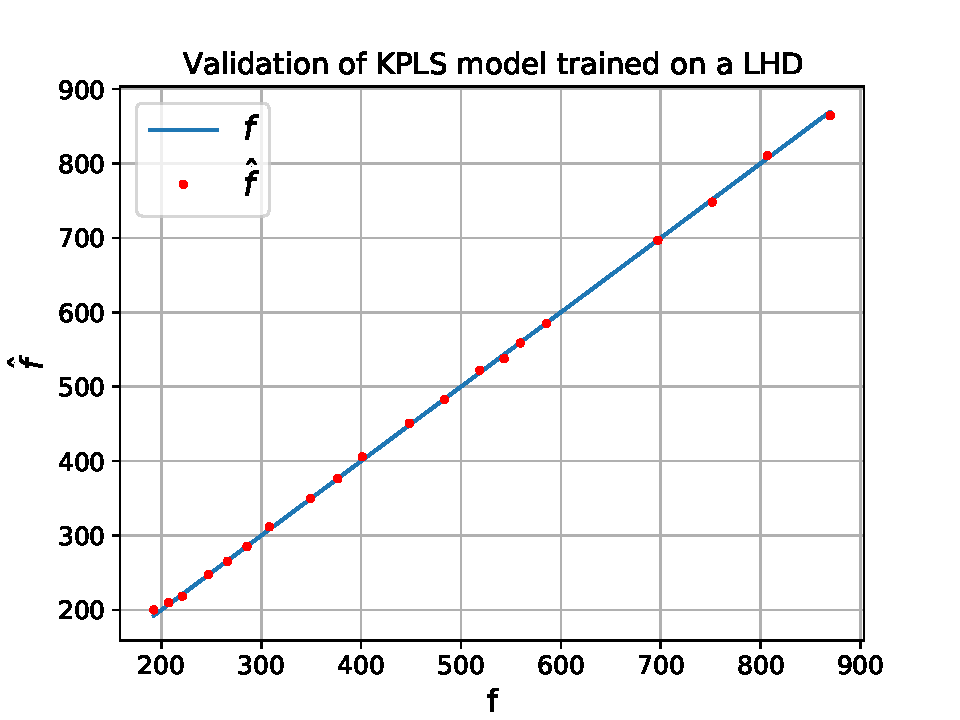
\includegraphics[width=\textwidth, height=0.8\textwidth]
    {Figure_36.pdf} 
    \end{subfigure}  
\hfill
\begin{subfigure}[b]{0.49\textwidth}
    \centering
    \caption{Factorial design, NRMSE = 0.010939}
    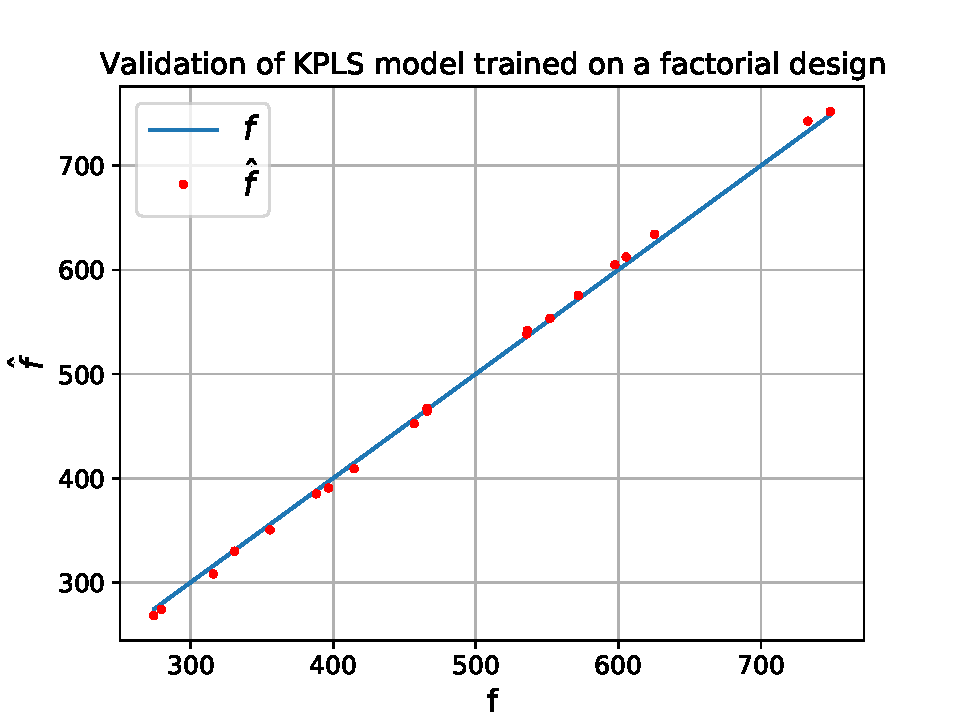
\includegraphics[width=\textwidth, height=0.8\textwidth]
    {Figure_37.pdf} 
    \end{subfigure}
\caption{NRMSE of metamodels trained on a LHD and a factorial 
design}     
\label{fig:LHD_FD_training}  
\end{figure}

\newpage
%------------------------------------------------------


The RMSE is calculated using the following equation:

\begin{equation}\label{RMSE_SOO}
RMSE = \sqrt{ \frac{\sum_{i=1}^{n_{val}} 
\left( \hat{f}_{i} - f_{i} \right)^2 }{n_{val}} }
\end{equation}
\\[0.1cm]
where $n_{val}$ is the number of validation points and   
$\vec{χ_{i}} = \left[ χ_{i,1}, \hdots, χ_{i,n_{β}} \right]
\!\in \!\mathbb{R}^{n_{β}}$ the vector of the $i_{th}$ 
training point. Validation points are selected from the design 
space via the implementation of any DoE technique and are used in 
the evaluation of the model\cite{preprint_SMT}. Every set of 
sample points different than the one used to train the metamodel 
is considered a set of validations point. The values obtained
via the use of the trained surrogate model are denoted by 
$\hat{f}$ and referred to as estimated values. In equation 
\ref{RMSE_SOO} the existence of a single objective is assumed and 
the both $f$ and $\hat{f}$ are scalar quantities. In MOO 
problems, the RMSE is computed w.r.t. to each objective 
iteratively. In order to remove the dependency on the order of 
magnitude Normalised Root Mean Square Error (NRMSE) is 
introduced, which can be calculated from the following formula:
\begin{equation}
NRMSE = \sqrt{ \dfrac{1}{n_{val}}\sum_{i=1}^{n_{val}} \left( 
\frac{ \hat{f}_{i} - f_{i}  }{f_{i}} \right)^2 }
\end{equation}
\\
NRMSE is dimensionless and assumes values in the $\mathbb{R}^{+}$, 
with values closer to zero indicating a well-trained metamodel.
NRMSE is not restricted in a specific dataset but can rather be
generalised to compare models of various orders of magnitude. 

In addition to inferior metamodel quality, factorial designs are 
imposed with severe limitations when sampling high-dimensional 
design spaces. Even in its simplest form a FFD must consist of 
$n_{doe} = 2^{n_{β}}$ possible combinations. In 10 dimensions, 
the number of runs required to fully replicate the design is:
$$ n_{doe} = (2)^{10} = 1024 $$ 

If moreover the case in study is that of a 3D airfoil, then 
each set of design variable values $\vec{β}$ would correspond 
to a different airfoil shape. That results in 1024 
different shapes and therefore to a beyond sustainability 
computational cost. The number of factorial runs needed for the
creation of a factorial design in 10-dimensional space is $n_{doe} 
> 600$, which results experimentally from the implementation Python 
software. On the other hand, LHS scheme is suitable for creating 
high-dimensional designs and offers a better coverage of the design 
space combined with minimal impact on the computational cost, which 
leads to its selection as the main sampling scheme used in this 
thesis. 
   
\newpage
%------------------------------------------------


\section{Communication between EASY and SMT in MAEAs with off-line training}


In the evaluation phase of MAEAs with off-line training the PSM is 
replaced by a surrogate model, which is trained on $n_{t}$ 
training patterns that are collected via the use of various DoE 
techniques. The creation of DoE, the training of the metamodel 
and the prediction of the objective function value are performed 
via the use of SMT. However, in order for SMT to facilitate the 
evolution performed by EASY (see appendix \ref{appendix:EASY}), a 
set of modifications must be applied in order for the two programs 
to be compatible. Responsible for the establishment of a line of 
communication between the two software is a Python script, which is 
manually created and can be decomposed in the following sections:

\begin{enumerate}
\item \textbf{Sampling (Code 1)} \\ 
The design space is defined, i.e. upper and lower bound 
of each design variable, along with the magnitude of the design, 
denoted by $n_{doe}^{'}$, and the DoE technique utilized to 
construct it. The $n_{doe}^{'}$ collected training patterns 
$\mathbf{X}$ are subsequently written in an ASCII text file 
\textit{sample\_points.dat}, prior to the termination of Code 1. 
 
\item \textbf{Evaluation of sample points on the PSM (Code 2)} \\
Code 2 contains the exact PSM. Both the input to the PSM, i.e. 
the observations $\mathbf{X} \! \in \!\mathbb{R}^{n_{doe}^{'} 
\times n_{β}}$ contained in \textit{sample\_points.dat}, and the 
yielded responses $\mathbf{F}(\vec{χ}) \!\in \!\mathbb{R}^{n_{doe}
^{'} \times n}$ are written in a plain ASCII text file 
\textit{model\_values.dat}, along with the constraints $\mathbf{C}
(\vec{χ}) = [\vec{c}_{1}, \vec{c}_{2}, \hdots, \vec{c}
_{n_{t}}]^{T}$, in case the optimization problem is constrained. 
Each component $\vec{c}_{i} = [c_{i,1}, c_{i,2}, \hdots, 
c_{i,n_{c}}]$ corresponds to the constraint vector $\vec{c}
(\vec{χ})$ of the $i_{th}$ sample point $\vec{χ} \in \mathbb{R}
^{n_{β}}$.

\item \textbf{Training of metamodel (Code 3)} \\
Codes 1 through 3 are incorporated in the 
\textit{preprocessor.exe} executable. Code 3 in particular is 
responsible for training the selected surrogate model. In order 
to accomplish that, first $n_{doe}^{'}$ $(\vec{χ}, \vec{f}
(\vec{χ}))$ observed pairs must be imported from 
\textit{model\_values.dat}. At the end of each off-line 
optimization cycle the MDB is updated with $λ_{e}$ elites that 
are contained in the $P_{e}$ set. Consequently, Code 3 is also 
responsible for incorporating $λ_{e}$ $(\vec{β},\vec{f}(\vec{β}))$ 
pairs in the training of the metamodel, after importing them from 
a plain ASCII text file \textit{out.log} that is created by Code 
6. Once the MDB is complete, a new surrogate model is trained at 
the start of each optimization cycle using $n_{t}$ training pairs 
$(\vec{χ},\vec{f}(\vec{χ}))$ (see eq. \ref{off_line_nt}). 

In the case of a constrained optimization, 
the matrix of constraints $\mathbf{C}(\vec{χ})$ is imported 
into Code 3 along with the objective function values 
matrix $\mathbf{F}(\vec{χ})$, and a distinct metamodel is 
trained on each constraint or a single metamodel is trained 
for the entirety of the imposed constraints. Metamodels 
trained on constraints require $n_{t}$ $(\vec{χ},\vec{c}
(\vec{χ}))$ training pairs to be built. 

Once the training is complete, the parameters of each trained 
metamodel are witten in a binary text file using the Python 
module \textit{.pickle()}; in this way, it can be utilized in 
the evaluation of prominent solutions in each generation of the 
evolution. For some metamodels, however, \textit{.pickle()} is not 
applicable, e.g. RBF. In that case, a folder containing the cached 
data that are produced via the training process is used in order 
to store and reuse the saved surrogate model. 

\item \textbf{Evaluation using the trained metamodel 
(Code 4)} \\ 
The current script uses as input the file \textit{task.dat}, which 
EASY creates, and contains a single offspring $\vec{β} \! \in \! 
P_{λ}^g$. A metamodel prediction $\hat{f}(\vec{β})$ is 
subsequently computed for every offspring $\vec{β} \in P_{λ}^g 
\subset \mathbb{R}^{n_{β}}$ by utilizing the stored 
metamodel via the use of \textit{.pickle()} module. Code 4 is 
identical in form to \textit{evaluation.exe}, but the PSM is 
replaced by a surrogate hence it is called 
\textit{prediction.exe}. 

\item \textbf{Selection of objectives and constraints 
(Code 5)} \\
In order to establish the communication between EASY and 
the user, \textit{postprocessor.exe} is manually created. 
This script is responsible for writing the objectives and the 
imposed constraints of the optimization in a \textit{task.cns} 
and a \textit{task.res} file, respectively. Text files 
\textit{task.res} and \textit{task.cns} contain the predictions 
$\hat{\vec{f}}(\vec{β})$ and $\hat{\vec{c}}(\vec{β})$, 
respectively,  of a single individual $\vec{β} \!\in \!P_{λ}^{g}$ 
and are read by EASY.  
 
\item \textbf{Evaluation of elites using the trained 
metamodel (Code 6)} \\
Code 6 performs the evaluation of the elite population 
$P_{e}$ using the exact PSM. The only difference with Code 2 is 
that the inputs $(\vec{β},\hat{\vec{f}}(\vec{β}))$, $(\vec{β},
\hat{\vec{c}}(\vec{β}))$, $\forall \vec{β} \in P_{e}$ are 
imported from \textit{out\_L1.log}, which is created by EASY at 
the end of each optimization cycle, and the corresponding exact 
PSM evaluations $(\vec{β},\vec{f}(\vec{β}))$, $(\vec{β},\vec{c}
(\vec{β}))$ are written in \textit{out.log}. Both these files 
follow ASCII text format.

\end{enumerate}
\newpage
%---------------------------------------------------
%-------------------------------------------------------

\chapter{MAEAs with on-line training}
On-line trained surrogate models are built in each 
generation of the evolution and hence this MAEAs method is 
described as dynamic. The most common approach is one 
that involves the implementation of a Low-Cost 
Pre-Evaluation (LCPE) process. LCPE is responsible for 
the selection of promising individuals via the 
implementation of local or global metamodels. The former 
are however more widely used, since they tend to 
approximate complex objectives function more effectively. 
MAEAs with metamodels trained on-line via LCPE phase can
subsequently decomposed in the following discrete steps:   
 
\begin{ONL}
\item \textbf{Implementation of EAs} \\
The initialization of LCPE phase requires the 
implementation of conventional EAs for a number of 
generations. Each untried individual $\vec{β} \!\in \!P_{λ}^{g}$ is 
evaluated on the PSM and subsequently archived in 
the DB. Once a user-defined minimum number of individuals 
has been stored in the DB, LCPE\cite{LCPE} phase initiates.

\item \textbf{Low-cost Pre-evaluation} \\
LCPE phase initiates by training on the fly a local 
surrogate model for each untried individual $\vec{β} \in 
P_{λ}^{g}$. The training of each metamodel in SOO problems 
requires the selection of an appropriate set of training 
patterns from the vicinity of each individual $\vec{β}$. 
In MOO problems more sophisticated algorithms 
are required. Such a method is developed by PCOpt/NTUA and is 
called Training Pattern Selection (TPS)\cite{TPS}. Using 
the trained local metamodels, the objective function value 
of each offspring s subsequently predicted and denoted by 
$\hat{\vec{f}}(\vec{β}), \forall \vec{β}\in P_{λ}^{g}$.

\item \textbf{Computation of fitness function} \\
This step is identical to step EAs-3. Each candidate 
solution $\vec{β} \!\in \!P_{λ}^{g}$,  is assigned a scalar 
value. Depending on the process implemented to evaluate 
each candidate solution, i.e. PSM or LCPE using local 
metamodels, the fitness function is either exactly 
calculated ($Φ(\vec{β})$) or predicted ($\widehat{Φ}
(\vec{β})$), respectively.

\begin{equation}
Φ(\vec{β}_{i}) = Φ(\vec{f}(\vec{β}_{i}), 
\{ \vec{f}(\vec{z}) \hspace{2mm} \vert \hspace{2mm}
\vec{z} \in P_{λ}^g \setminus \{\vec{β}_{i}\} \}) \in 
\mathbb{R} \hspace{3mm} ,\text{for} \hspace{2mm} i=1,λ
\end{equation}
or
\begin{equation}
\widehat{Φ}(\vec{β}_{i}) = \widehat{Φ}(\hat{\vec{f}}
(\vec{β}_{i}), \{ \hat{\vec{f}}(\vec{z}) \hspace{2mm} 
\vert \hspace{2mm}
\vec{z} \in P_{λ}^g \setminus \{\vec{β}_{i}\} \}) \in 
\mathbb{R} \hspace{3mm} ,\text{for} \hspace{2mm} i=1,λ
\end{equation}

\newpage
%--------------------------------------------------------

\item  \textbf{Identification of elites}\\
The values of the fitness function assigned to each 
candidate solution are used to update the temporary set 
of elites $P_{e}$. In SOO problems $Φ(\vec{β}) \! \equiv 
\! f(\vec{β})$, $\widehat{Φ}(\vec{β}) \equiv 
\hat{f}(\vec{β})$ and there is only one optimal 
solution $λ_{e}\! = \! 1$. In MOO problems the best 
$λ_{e} \! < \! λ$ offspring are selected to populate the 
$P_{e}$ set. In the latter category due to the large 
number of data the fitness function values are assigned 
via the implementation of the simplest sorting algorithm, 
e.g. NSGA\cite{NSGA} or SPEA\cite{SPEA}, or via a simple 
ranking of non-dominated Pareto fronts. The final $P_{e}$ 
set is formed as such:
\begin{equation}
P_{e} \triangleq \lbrace \vec{β}_{i} \!: \widehat{Φ}
(\vec{β}_{i}) < \widehat{Φ}(\vec{z}), \vec{z} \in 
P_{λ}^{g} \setminus P_{e} \rbrace
\hspace{3mm} ,\text{for} \hspace{2mm} i=1,λ_{e}
\end{equation}

The process of populating the $P_{e}$ set continues until:
\begin{equation}
 λ_{e,min} < λ_{e} < λ_{e,max} 
\end{equation}  

where $λ_{e,min}, λ_{e,max}$ are user-defined lower and 
upper bounds of the number of elites $λ_{e}$, 
respectively.

\item \textbf{CFD evaluation}\\
Subsequently, $λ_{e}$ elite candidate solutions contained 
in the $P_{e}$ set are re-evaluated on the PSM and are stored in 
the DB. Depending on the deviation between metamodel and 
psm evaluated outcome, denoted by $ε_{P_{e}}$, either the 
evolution continues or new elites are selected (step 
ONL-4) and re-evaluated (step ONL-5). This criterion can
be expressed mathematically as such:
\begin{equation}
ε_{P_{e}} = \left| \dfrac{\vec{f}(\vec{β}) - 
\hat{\vec{f}}(\vec{β})}{\vec{f}(\vec{β})} \ \right| < 
ε_{λ} \hspace{3mm} ,\forall \vec{β} \in P_{e} 
\end{equation}

where $ε_{λ}$ a user-defined value upon which the 
criterion is satisfied. 

\item \textbf{Elitism}\\
The temporary set $P_{e}$ is used to update the population of 
the current generation $P_{α}^{g}$. The process of elitism
subsequently commences and leads to the formation of 
$P_{α}^{g+1}$ set. This step is identical to step EAs-5.   

\item \textbf{Crossover and mutation}\\
Crossover and mutation operators are applied to form the
set $P_{λ}^{g+1}$, similarly to step EAs-6. 

\item \textbf{Termination}\\
Once the process of implementing evolution operators is 
complete, the convergence of the on-line training process 
is tested. If a user-defined number of generations
has been formed the process terminates, alternatively, 
the next generation initiates by setting $g = g + 1$. If a
user-defined number of idle generations $n_{idle}$ has been 
performed using metamodels in LCPE phase, then plain EAs are 
utilized and the counter of idle LCPE generations $c_{idle}$ is 
reset to zero, as shown in figure \ref{fig:online_flowchart}. 
\end{ONL}

\newpage
%-------------------------------------------------------

\begin{figure}[h!]
\centering
\begin{center}
\begin{adjustbox}{width=1.0\textwidth,height= 
0.92\textheight,keepaspectratio}
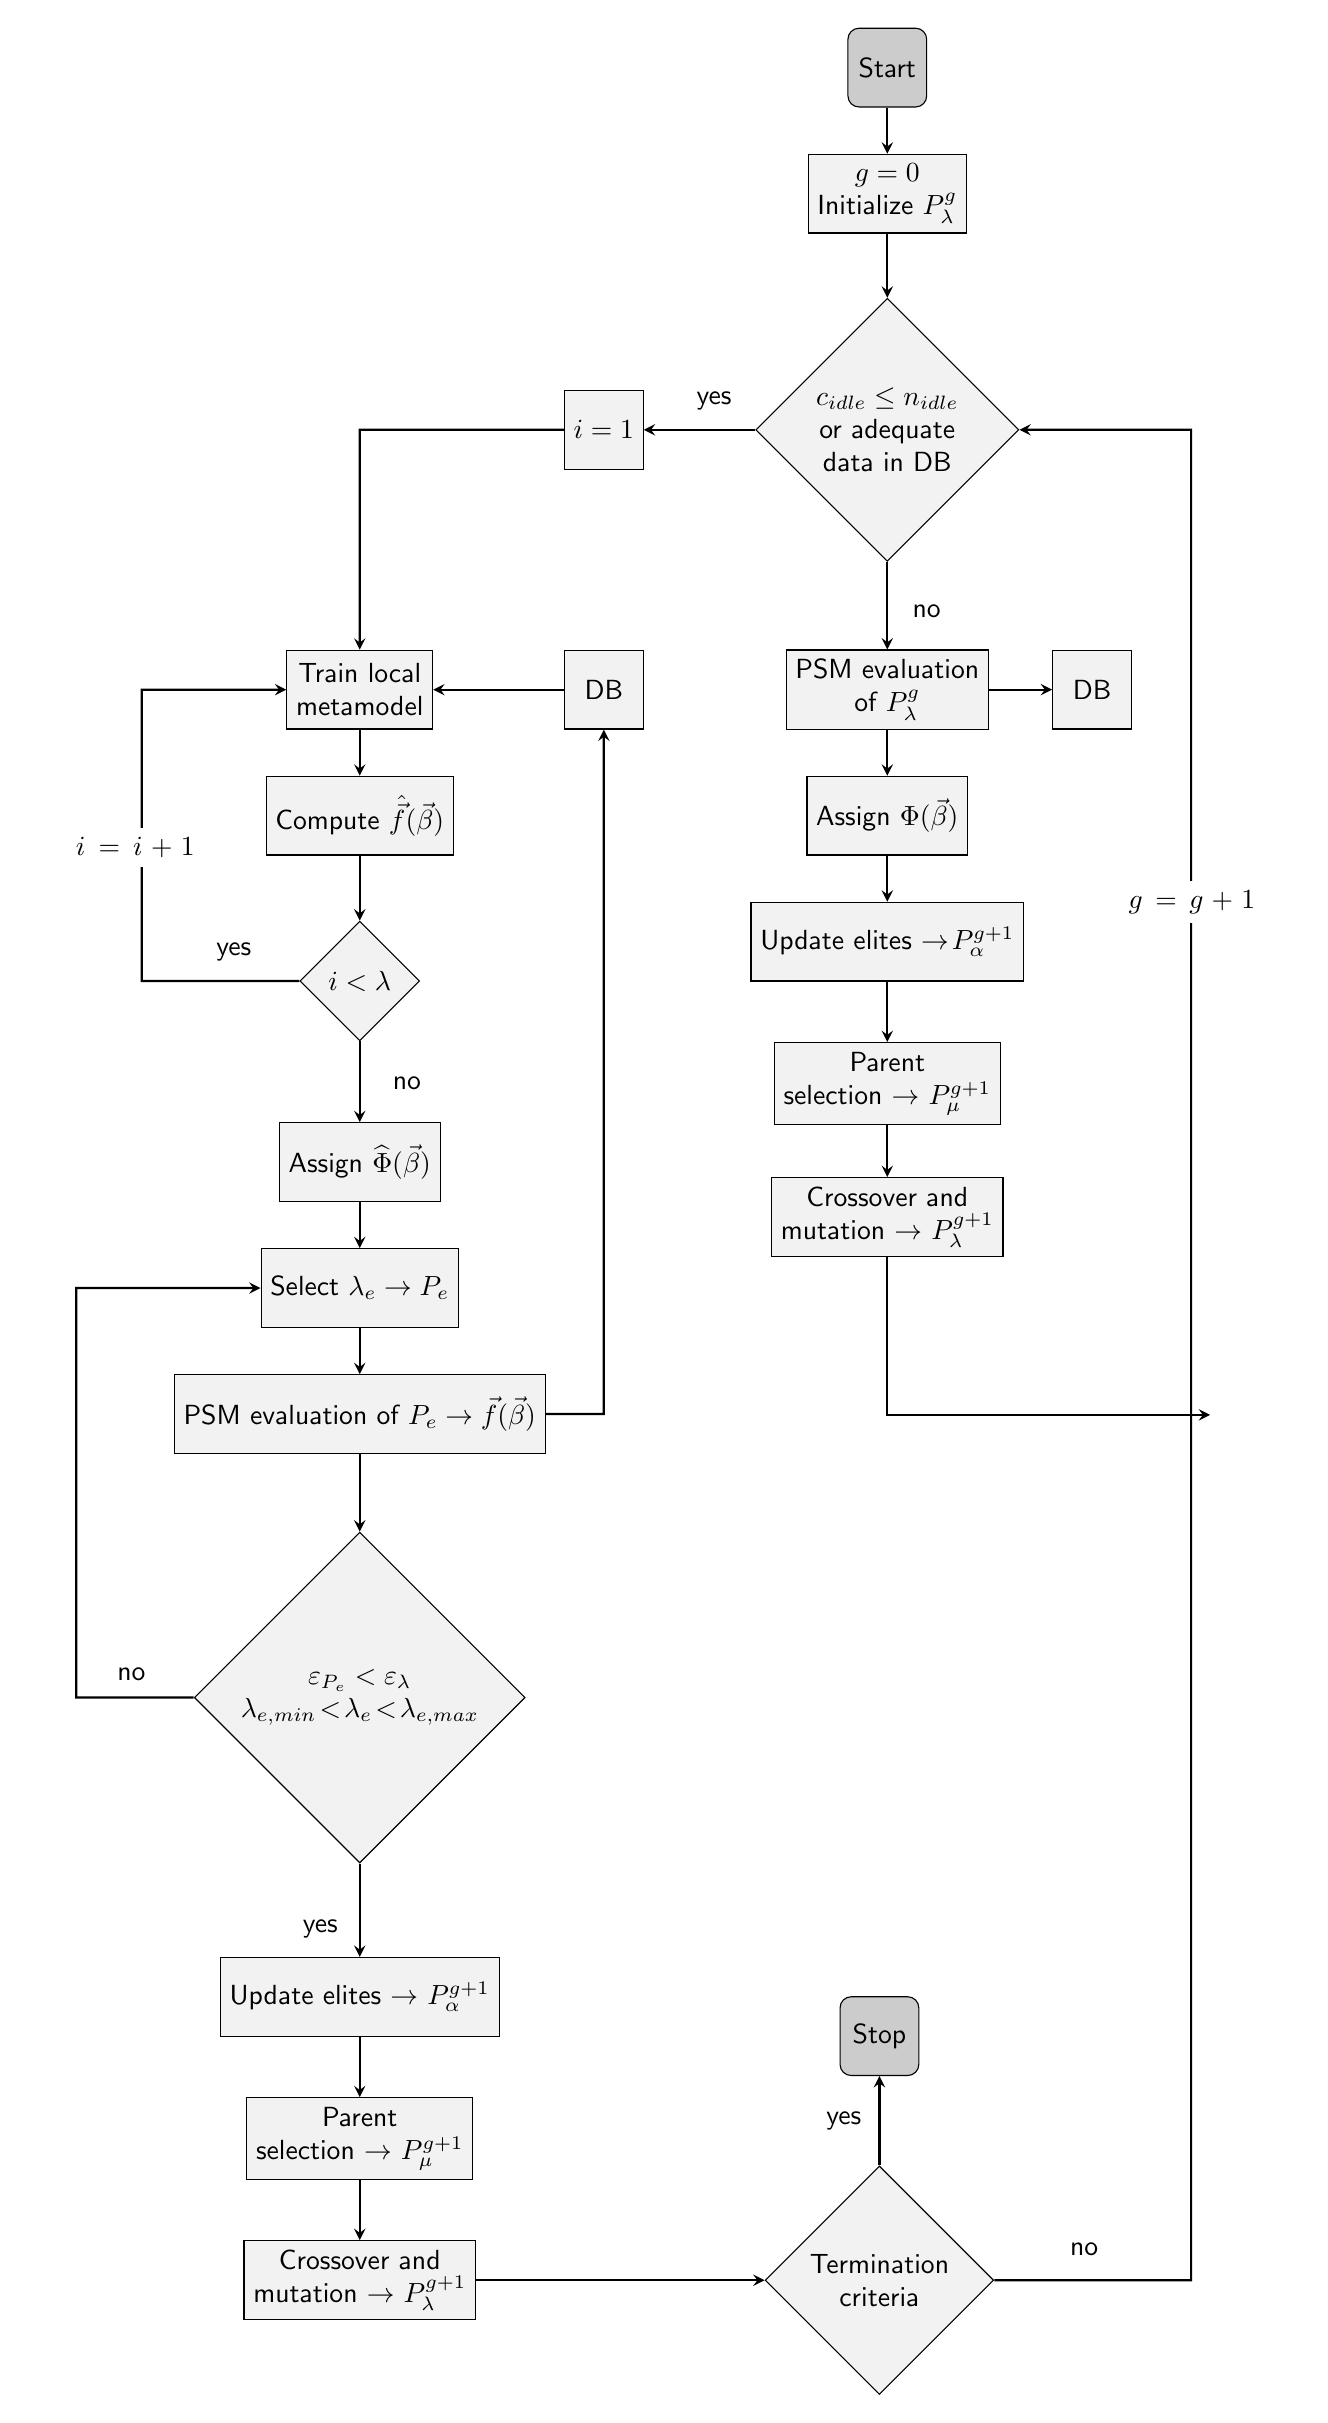
\begin{tikzpicture}[node distance=1.6cm,
    every node/.style={fill=white, font=\sffamily}, 
    align=center]
    
\node (start) [startstop] {Start};

\node (pro2) [process, below of=start]
{$g = 0$ \\ Initialize $P_{λ}^{g}$};

\node (dec2) [decision, below of=pro2, yshift=-1.4cm] 
{$c_{idle} \leq n_{idle}$ \\ or adequate \\ data in DB };

\node (pro3) [process, below of=dec2, yshift=-1.7cm] 
{PSM evaluation \\ of $P_{λ}^{g}$};

\node (DB) [process, left of=pro3, xshift=-2cm] 
{DB};

\node (DB2) [process, right of=pro3, xshift=1cm] 
{DB};

%--------------------------------------------------
%-------LCPE phase-------------------
\node (LCPE1) [process, left of=dec2, xshift=-2cm] 
{$i = 1$};

\node (LCPE2) [process, left of=DB, xshift=-1.5cm] 
{Train local \\ metamodel};

\node (LCPE3) [process, below of=LCPE2, yshift=0cm] 
{Compute $\hat{\vec{f}}(\vec{β})$};

\node (dec3) [decision, below of=LCPE3, yshift=-0.5cm] 
{$i < λ$};

\node (LCPE4) [process, below of=dec3, yshift=-0.7cm] 
{Assign $\widehat{Φ}(\vec{β})$};

\node (LCPE5) [process, below of=LCPE4, yshift=0cm] 
{Select $λ_{e} \rightarrow P_{e}$};

\node (LCPE6) [process, below of=LCPE5, yshift=0cm] 
{PSM evaluation of $P_{e} \rightarrow \vec{f}(\vec{β})$};

\node (dec4) [decision, below of=LCPE6, yshift=-2cm] 
{$ε_{P_{e}} < ε_{λ}$ \\ 
$λ_{e,min} \!< \!λ_{e} \!< \!λ_{e,max}$};

\node (LCPE7) [process, below of=dec4, yshift=-2.2cm] 
{Update elites $\rightarrow$ $P_{α}^{g+1}$};

\node (LCPE9) [process, below of=LCPE7, yshift=-0.2cm] 
{Parent \\ selection $\rightarrow$ $P_{μ}^{g+1}$};

\node (LCPE8) [process, below of=LCPE9, yshift=-0.2cm] 
{Crossover and \\ mutation $\rightarrow$ $P_{λ}^{g+1}$};


%-------------------------------------------------------

\node (pro4) [process, below of=pro3, yshift=-0.0cm] 
{Assign $Φ(\vec{β})$};

\node (pro5) [process, below of=pro4] 
{Update elites $\rightarrow \!P_{α}^{g+1}$};

\node (pro6) [process, below of=pro5, yshift=-0.2cm]
{Parent \\ selection $\rightarrow$ $P_{μ}^{g+1}$};

\node (pro7) [process, below of=pro6, yshift=-0.1cm] 
{Crossover and \\ mutation $\rightarrow$ $P_{λ}^{g+1}$};
 
\node (dec1) [decision, right of=LCPE8, xshift=5cm] 
{Termination \\ criteria};
\node (stop) [startstop, above of=dec1, yshift=1.5cm]
{Stop};

\draw [arrow] (start) -- (pro2);
\draw [arrow] (pro2) -- (dec2);
\draw [arrow] (dec2) -- (LCPE1);
\draw [arrow] (dec2) -- (pro3);
\draw [arrow] (pro3) -- (DB2);
\draw [arrow] (DB) -- (LCPE2);
\draw [arrow] (LCPE2) -- (LCPE3);
\draw [arrow] (LCPE3) -- (dec3);
\draw [arrow] (dec3) -- (LCPE4);
\draw [arrow] (LCPE4) -- (LCPE5);
\draw [arrow] (LCPE5) -- (LCPE6);
\draw [arrow] (LCPE6) -- (dec4);
\draw [arrow] (dec4) -- (LCPE7);
\draw [arrow] (LCPE7) -- (LCPE9);
\draw [arrow] (LCPE9) -- (LCPE8);
\draw [arrow] (LCPE8) -- (dec1);
\draw [arrow] (pro3) -- (pro4);
\draw [arrow] (pro4) -- (pro5);
\draw [arrow] (pro5) -- (pro6);
\draw [arrow] (pro6) -- (pro7);


%----------arrow for pro7----------------
\draw [->][arrow] (pro7.south) -- ++(0,-2) -- ++(4.1,0);

%----------arrow for dec1----------------
\draw [arrow] (dec1) -- node[anchor=east, xshift=-0.1cm] 
{yes} (stop);
\draw [->][arrow] (dec1.east) -- ++(2.5,0) -- ++(0,23.5) 
-- ++(-2,0) -- node[xshift=2.1cm,yshift=-6cm, text 
width=2.5cm]{$g = g +1 $}(dec2.east);
\draw (2.5,-27.5) node[anchor=north]{no};

%-----------arrow for dec2--------------
\draw (0.5,-6.7) node[anchor=north]{no};
\draw (-2.2,-4) node[anchor=north]{yes};

%----------arrow for LCPE1-------------
\draw [arrow] (LCPE1) -- ++(-3.1,0) -- (LCPE2.north);

%----------arrow for dec3----------------
\draw (-6.1,-12.7) node[anchor=north]{no};
\draw [->][arrow] (dec3.west) -- ++(-2,0) -- ++(0,1) 
-- ++(0,2.7) -- node[xshift=-1cm,yshift=-2cm, text 
width=2.5cm]{$i = i +1 $}(LCPE2.west);
\draw (-8.3,-11) node[anchor=north]{yes};

%-----------arrow for LCPE6-------------
\draw [arrow] (LCPE6) -- ++(3.1,0) -- (DB.south);

%-----------arrow for dec4------------
\draw [arrow] (dec4) -- ++(-3.6,0) -- ++(0,5.2) --
(LCPE5.west);
\draw (-7.2,-23.4) node[anchor=north]{yes};
\draw (-9.6,-20.2) node[anchor=north]{no};

\end{tikzpicture}
\end{adjustbox}
\end{center}
\caption{Flowchart of MAEAs using on-line trained 
metamodels}
\label{fig:online_flowchart}
\end{figure}


\newpage
%------------------------------------------------------

\section{Communication between EASY and SMT in MAEAs with on-line training}
The optimization based on MAEAs via the use of 
EASY\cite{EASY} software is primarily focused on training 
metamodels on-line and therefore a number of metamodels 
are already archived in the database of EASY. In order to
provide EASY with external metamodels trained on SMT 
software, the following Python scripts must be deployed:

\begin{enumerate}

\item \textbf{ Evaluation of offspring using the exact 
model (Code 1)} \\
This script contains the exact PSM and is responsible for 
computing the exact objective function vector $\vec{f}(\vec{β}), 
\forall \vec{β} \in P_{λ}^{g}$. Each one of those candidate 
solutions is imported from the file \textit{task.dat}. The script 
is subsequently converted to an executable process, called 
\textit{evaluation.exe}, and executed via \textit{task.bat} batch 
file, which has the following structure:

\begin{lstlisting}[language = command.com, caption = Structure of 
\textit{task.bat} file that initiates the exact evaluation of 
offspring]
@echo off
erase results.dat 
evaluation.exe > nul 
postprocessor.exe > nul
\end{lstlisting}

\item \textbf{Training of metamodel (Code 2)} \\
LCPE phase initiates by training a local metamodel for 
each individual $\vec{β} \in P_{λ}^{g}$. Both the $n_{t}$ 
training patterns $\mathbf{X}$ and their corresponding exact 
model values $\mathbf{F}(\vec{χ})$ are imported from a plain 
ASCII text file, which is called \textit{meta.db} and is 
created by EASY. Code 2 is converted to \textit{train.exe} 
and executed via a user-created batch file 
\textit{meta\_train.bat} that has the following structure:

\begin{lstlisting}[language = command.com, caption =Structure of 
\textit{meta\_train.bat} file that initiates training of the 
metamodel]
@echo off
train.exe > nul 
\end{lstlisting}

\item \textbf{Evaluation of offspring using the metamodel 
(Code 3)} \\
Code 3 utilises each local metamodel, which is built 
in the vicinity of the $i_{th}$ individual $\vec{β}_{i} \!\in 
\!P_{λ}^{g}$, in order to produce the evaluation 
$\hat{\vec{f}}(\vec{β}_{i})$. Each individual is 
contained in a plain ASCII text file \textit{meta.dat}, 
which is structured similarly to \textit{task.dat}. 
Consequently, after converting the script to an executable 
\textit{prediction.exe} Code 3 is executed iteratively
for $λ$ offspring via \textit{meta\_use.bat} batch file, 
which has the following structure: 

\begin{lstlisting}[language = command.com, caption = Structure of 
\textit{meta\_use.bat} file that initiates the evaluation of some 
candidate solution $\vec{β} \!\in \! P_{λ}^{g}$ based on its 
personalised local metamodel]
@echo off
erase results.dat 
prediction.exe > nul 
postprocessor.exe > nul
\end{lstlisting}


\newpage
%--------------------------------------------------------

\item \textbf{Objectives and constraints (Code 4)} \\
Code 4, which is called \textit{postprocessor.exe}, is executed 
alternately via \textit{task.bat} and \textit{meta\_use.bat} 
batch files in order to provide EASY with the exact $\vec{f}
(\vec{β})$ or predicted \scalebox{0.86}{%
$\hat{\vec{f}}(\vec{β})$ } objective function value of each 
individual $\vec{β} \in P_{λ}^{g}$, respectively. EASY expects to 
read this value, or values if there are more than one objective, 
in \textit{task.res} file. Any constraint $\vec{c}(\vec{β})$ is 
subsequently written in a \textit{task.cns} file.  

\end{enumerate}

In EASY, the MAEA-based on-line construction process consists of 
the same fundamental steps, i.e. evaluation based on the PSM, 
training of the surrogate model and prediction based on the trained 
model, but no additional user-constructed scripts are needed to 
utilize the built-in metamodels of EASY, in contrast to SMT.   
 
\newpage
%------------------------------------------------------------------
%--------------------------------------------------------

\chapter{Surrogate Models}
\label{chapter:models}
Metamodels approximate the initial evaluation model by 
utilising a data-driven approach, which is based on 
statistical analysis of the observed data. Consequently, the 
selection of a suitable surrogate model is essential in the optimal 
utilization of MAEA-based optimization. In attempt to achieve 
homogeneity throughout this thesis, it is reminded that 
the observations' matrix formed of $n_{t}$ training 
patterns is denoted by $\mathbf{X} = [\vec{χ}_{1}, 
\vec{χ}_{2}, \hdots, \vec{χ}_{n_{t}}]^T$, where each 
component $\vec{χ}_{i} = [χ_{i,1}, χ_{i,2},\hdots, 
χ_{i,n_{β}}]$ represents an observation $\vec{χ} \in \mathbb{R}
^{n_{β}}$. Their corresponding objective function
values are included in matrix $\mathbf{F}(\vec{χ}) = 
[\vec{f}_{1}, \vec{f}_{2}, \hdots, \vec{f}_{n_{t}}]^{Τ}$, 
where each component $\vec{f}_{i} = [f_{i,1}, f_{i,2}, 
\hdots, f_{i,n}]$ represents a response $\vec{f} \in 
\mathbb{R}^{n_{β}}$. In order to simplify the mathematical 
equations describing the surrogate models, $\mathbf{F}
(\vec{χ})$ is reduced to an 1-dimensional matrix  by 
assuming, without loss in generality, that the optimization 
process has a single objective. From there, the 
respective equations describing a MOO can be easily formulated by 
combining the SOO equations iteratively for $n$ objectives. In 
SOO, therefore, $\mathbf{F}(\vec{χ}) \!= \!\mathbf{F} \!= [f_{1}, 
f_{2}, \hdots, f_{n_{t}} ]^{T} \!\in \!\mathbb{R}^{n_{t}}$. 
Surrogate models are used to predict the objective function value 
$f(\vec{β})$ at any untried location of the design space, i.e. at 
each candidate solution $\vec{β} \in \mathbb{R}^{n_{β}}$. 
The theoretical background of every metamodel utilized via SMT in 
this thesis is subsequently presented. 


\vfill
\section{Kriging}
Kriging\cite{Kriging} is a surrogate model used for 
predicting the objective function value at any candidate
solution $\vec{β} \in \mathbb{R}^{n_{β}}$ in the design space. 
In order to make the prediction Kriging uses an interpolation 
method that combines a deterministic term with the realization of 
stochastic process. The former is replaced by a regression model 
and the latter is the realization of the stationary process 
Gaussian $z(\vec{β}) \!\backsim \!N(0,C)$ with a zero mean 
and a covariance kernel $C(\vec{β})$ of the observations:
\begin{equation}
C(\vec{χ}_{i}, \vec{χ}_{j}) = σ^{2} R(\vec{χ}_{i}, \vec{χ_{j}})
\end{equation} 
\\[-0.5cm]
where $σ^2$ the variance of the process and $R( \vec{χ_{i}}, 
\vec{χ_{j}})$ the correlation between any two observations
$\vec{χ_{i}}, \vec{χ_{j}} \!\in \!\mathbb{R}^{n_{β}}, \forall i,j 
\in [1,n_{t}]$. In order to improve the fitting of the Kriging 
model the distribution of training patterns in each problem 
dimension is normalized:
\begin{equation}
\vec{χ}_{norm} = \dfrac{\vec{χ} - μ_{\vec{χ}^{(j)}} }
{σ_{\vec{χ}^{(j)}}}
\end{equation} 

\newpage
%------------------------------------------------------------

\vspace{1mm} 
where $\vec{χ}^{(j)} \!= \! [χ_{1,j}, χ_{2,j}, 
\hdots, χ_{n_{t},j} ]^{T} \! \in \! \mathbb{R}^{n_{t}}$ is the 
column vector of the $n_{t} \times n_{β}$ matrix $\mathbf{X}$ 
and $μ_{\vec{χ}^{(j)}}$, ${σ_{\vec{χ}^{(j)}}}$ the mean 
value and the standard deviation of the $j_{th}$ observation, 
respectively. The correlation between any normalized 
training point $\vec{{χ}}_{norm} \!\in \!S \!\subset \!\mathbb{R}
^{n_{β}}$, where $S$ is the design set, can be computed using one 
of the following correlation kernels \footnote{In all Kriging 
models from this point on, the notation of normalization will not 
be used for sampled points but will be implied for simplicity, so 
$\vec{χ} \equiv \vec{{χ}}_{norm}$ and $\vec{χ} \equiv \vec{{χ}}
_{norm}$} \cite{preprint_SMT,Matern}:

\begin{itemize}
\item Exponential Ornstein-Uhlenbeck process
\begin{equation}\label{Oberstein correlation}
R \left( \vec{χ_{i}}, \vec{χ_{j}} \right) = 
\prod_{l=1}^{n_{β}}exp \left( -\theta_{l} 
\left| χ_{i,l} - χ_{j,l} \right| \right)
\end{equation}
              
\item Gaussian
\begin{equation}\label{Gaussian correlation}
R \left( \vec{χ_{i}}, \vec{χ_{j}} \right)  = 
\prod_{l=1}^{n_{β}}exp \left(-\theta_{l} 
\left( χ_{i,l} - χ_{j,l} \right)^2  \right)
\end{equation}  

\item Mat\'ern 5/2
\begin{equation}
R \left( \vec{χ_{i}}, \vec{χ_{j}} \right)  = 
\prod_{l=1}^{n_{β}} \left(\! 1 + \sqrt{5}\left|χ_{i,l} -
χ_{j,l} \right| + \dfrac{5}{3} θ_{l}^2\left( χ_{i,l} -
χ_{j,l} \right)^2 \right)\! exp\! \left(\!-\sqrt{5}θ_{l} 
\left| χ_{i,l} - χ_{j,l} \right|\right)
\end{equation}

\item Mat\'ern 3/2
\begin{equation}
R \left( \vec{χ_{i}}, \vec{χ_{j}} \right)  = 
\prod_{l=1}^{n_{β}} \left(\! 1 + \sqrt{3} θ_{l}
\left|χ_{i,l} - χ_{j,l} \right| \right) 
exp\! \left(\!-\sqrt{3}θ_{l} \left| χ_{i,l} - χ_{j,l} 
\right|\right)
\end{equation}
\end{itemize}
\vspace{1mm}
where $θ_{l}$ are parameters that denote the degree of 
correlation between training points w.r.t. each design 
dimension $l \in [1,n_{β}]$. Kriging assumes that the estimated 
value of each correlation parameter $θ$ is constant for each 
independent design variable and therefore for each design 
dimension, leading to the creation of an isotropic 
model\cite{Kriging1}. The correlation patterns of the observed 
data and their corresponding covariance can be stated in the form 
of an orthogonal matrix $\mathbf{R}$ and $\mathbf{C}$, 
respectively:
\begin{equation}
\textbf{R} = 
	\begin{bmatrix}
	R(\vec{χ}_{1}, \vec{χ}_{1}) & \hdots & 
	R(\vec{χ}_{1}, \vec{χ}_{n_{t}})
	\\
	\vdots & \ddots & \vdots
	\\
	R(\vec{χ}_{n_{t}}, \vec{χ}_{1}) & \hdots & 
	R(\vec{χ}_{n_{t}}, \vec{χ}_{n_{t}})
	\end{bmatrix} 
, \hspace{3mm} \mathbf{C} = 
\begin{bmatrix}
	C(\vec{χ}_{1}, \vec{χ}_{1}) & \hdots & 
	C(\vec{χ}_{1}, \vec{χ}_{n_{t}})
	\\
	\vdots & \ddots & \vdots
	\\
	C(\vec{χ}_{n_{t}}, \vec{χ}_{1}) & \hdots & 
	C(\vec{χ}_{n_{t}}, \vec{χ}_{n_{t}})
\end{bmatrix}
\end{equation} 

Under the assumption of a SOO problem, the Kriging model computes 
the objective function value at any normalized point $\vec{β} \in 
\mathbb{R}^{n_{β}}$ outside the sampled design as such:
\begin{equation}\label{Kriging_model_function}
f(\vec{β}) = μ_{Κ} + z(\vec{β})
\end{equation}
\\[-0.4cm]
where the deterministic term  $μ_{Κ}$ is expressed as a constant, 
linear or quadratic regression model:
\begin{equation}\label{deterministic_term}
μ_{Κ} = \sum_{j=1}^{k} \mathrm{w}_{j} p_{j}(\vec{β})
\end{equation}

\newpage
%--------------------------------------------------------


where $\mathrm{w} _{j}$ is the $j_{th}$ regression coefficient and 
$p_{j}: \mathbb{R}^{n_{β}} \mapsto \mathbb{R}$ are $k$ chosen 
functions. The parameter $k$ assumes various values to denote a 
constant, a linear or a quadratic regression model 
\cite{regression_model}. In a constant regression model, $k=1$ and 
$p_{1}(\vec{β}) \!= \!1$.  In a linear regression model, $k \!= \!
n_{β}+ 1$ and the corresponding functions assume the following 
values:

\begin{equation}
p_{1}(\vec{β}) = 1, \hspace{1mm} p_{2}(\vec{β}) = β_{1}, \hdots, 
\hspace{1mm} p_{k}(\vec{β}) = β_{n_{β}} 
\end{equation}
\\[-0.22cm]
In a quadratic regression model, $k=\dfrac{1}{2}(n_{β}+1)
(n_{β}+2)$ and the functions $p_{j}$ assume the following values:
\begin{equation}
\begin{split}
& p_{1}(\vec{β}) = 1, \hspace{2mm} 
p_{2}(\vec{β}) = β_{1}, \hdots,
\\ &
p_{n_{β}+1}(\vec{β}) = β_{n_{β}}, \hspace{2mm}
p_{n_{β}+2}(\vec{β}) = β_{1}^{2}, \hdots,
\\ &
p_{2n_{β}+1}(\vec{β}) = β_{1} β_{n_{β}}, 
\hspace{2mm}
p_{2n_{β}+2}(\vec{β}) = β_{2}^{2}, \hdots,
\\ &
p_{3n_{β}}(\vec{β}) = β_{2} β_{n_{β}}, \hdots
\\&
p_{k}(\vec{β}) = β_{n_{β}}^2
\end{split}
\end{equation}
\\[-0.2cm]
where $β_{j}\! \in \!\mathbb{R}$ is the component of any untried
point $\vec{β} \hspace{1mm}$ w.r.t. the $j_{th}$ design dimension 
for $j\! \in\! [1,n_{β}]$. 

\vspace{0.6cm}

\begin{itemize}
\item \textbf{Prediction with noise-free observations}
\end{itemize}

Kriging, when provided with the observed data that are collected 
via the implementation of DoE, can predict the value of any 
individual at any untried location of the design space 
accompanied by the measure of confidence of the prediction at 
that location. Under the assumption of a SOO problem, consider 
the linear predictor $\hat{f}(\vec{β})$ of the objective function 
at any untried point $\vec{β}$, given the prior observations 
$\mathbf{F} = [\vec{f}_{1}, \vec{f}_{2}, \hdots, \vec{f}
_{n_{t}}]^{T}$:
\begin{equation}\label{initial_linear_predictor}
\hat{f}(\vec{β}) = \vec{c}^{\hspace{1mm} T}(β) \mathbf{F} 
\end{equation}
\\[-2mm]
where $\vec{c}(β) \in \mathbb{R}^{n_{t}}$ is the $n_{t} \times 1$ 
vector of coefficients. Then the deviation between the predictor 
and the true objective function value:
\begin{equation}\label{linear_predictor}
\begin{split}
\hat{f}(\vec{β}) - f(\vec{β})& =  
\vec{c}^{\hspace{1mm} T}(\vec{β}) \mathbf{F} - ( μ_{Κ} + 
z(\vec{β})) \xrightarrow[(\ref{deterministic_term})]
{(\ref{Kriging_model_function})}
\\ &
= \vec{c}^{\hspace{1mm} T}(\vec{β}) \left( \mathbf{P}
\vec{\mathrm{w}} + \mathbf{Z} \right) - 
( \vec{p}^{\hspace{1mm} T}(\vec{β}) \vec{\mathrm{w}} + z(\vec{β}) )
\\ &
= \vec{c}^{\hspace{1mm} T}(\vec{β}) \mathbf{Z} - z(\vec{β}) +
( \mathbf{P}^{T} \vec{c}(\vec{β}) - \vec{p}(\vec{β}) )^{T} 
\vec{\mathrm{w}} 
\end{split}
\end{equation}
\\[1mm]
where $\mathbf{Z} = [z_{1}, z_{2}, \hdots, z_{n_{t}}]^{T}$ is the 
$n_{t} \times 1$ vector of errors at the observed points, 
$z(\vec{β})$ is the error at the untried location,
$\vec{p}(\vec{β}) = [p_{1}(\vec{β}), p_{2}(\vec{β}), \hdots, 
p_{k}(\vec{β})]^{T}$ is the $k \times 1$ vector of the chosen 
functions at any untried input $\vec{β}$ and $\mathbf{P}$ the 
corresponding $n_{t} \times k$ matrix for the complete design of 
observed data, which for $i = 1,n_{t}$ training patterns $\vec{χ}
_{i} \! = \! [χ_{i,1}, χ_{i,2}, \hdots, χ_{i,n_{β}}] \! \in \! S 
\!\subset \!\mathbb{R}^{n_{β}}$ is expressed as:


\newpage
%------------------------------------------------------------


\begin{equation}\label{polynomial_matrix}
\mathbf{P} = 
\begin{bmatrix}
p_{1}(\vec{χ}_{1}) & p_{2}(\vec{χ}_{1}) & \ldots 
&  p_{k}(\vec{χ}_{1}) 
\\
p_{1}(\vec{χ}_{2}) & p_{2}(\vec{χ}_{2}) & \ldots 
&  p_{k}(\vec{χ}_{2}) 
\\
\vdots & \vdots & \ddots & \vdots 
\\
p_{1}(\vec{χ}_{n_{t}}) & p_{2}(\vec{χ}_{n_{t}}) & \ldots 
&  p_{k}(\vec{χ}_{n_{t}}) 
\end{bmatrix}
%=
%\begin{bmatrix}
%1 & χ_{1,1} & \ldots &  χ_{1,n_{β}} 
%\\
%1 & χ_{2,1} & \ldots &  χ_{2,n_{β}} 
%\\
%\vdots & \vdots & \ddots & \vdots 
%\\
%1 & χ_{n_{t},1} & \ldots &  χ_{n_{t},n_{β}} 
%\end{bmatrix}
\end{equation}
\\[-3mm]

The best linear unbiased predictor (BLUP) is obtained by 
selecting the vector $\vec{c}(\vec{β})$ that minimizes the mean 
squared error (MSE). In order to keep the predictor 
unbiased, we demand that the expected value of the predictor 
and objective function coincides at the design sites $\mathbf{X}$
\cite{BLUP}:
\begin{equation}\label{constraint_BLUP}
\begin{split}
& E[\hat{f}(\vec{β}) - f(\vec{β})] = 0 
\xrightarrow{(\ref{linear_predictor})}
E[\vec{c}^{\hspace{1mm} T}(\vec{β}) \mathbf{Z} - z(\vec{β}) +
( \mathbf{P}^{T} \vec{c}(\vec{β}) - \vec{p}(\vec{β}))^{T} 
\vec{\mathrm{w}} ] = 0 \rightarrow
\\ & 
\vec{c}^{\hspace{1mm} T}(\vec{β})E[\mathbf{Z}] - E[z(\vec{β})] +
E[( \mathbf{P}^{T} \vec{c}(\vec{β}) - \vec{p}(\vec{β}))^{T} 
\vec{\mathrm{w}} ] = 0 
\xrightarrow{E[z(\vec{β})] = μ_{z} = 0}
\\ &
E[( \mathbf{P}^{T} \vec{c}(\vec{β}) - \vec{p}(\vec{β}))^{T}] 
\vec{\mathrm{w}}  = 0 
\rightarrow
\mathbf{P}^{T} \vec{c}(\vec{β}) - \vec{p}(\vec{β}) = 0
\end{split}
\end{equation}
\\
Consequently, the MSE of the predictor is calculated as such:
\begin{equation}\label{BLUP_predictor}
\begin{split}
E[\hat{f}(\vec{β})] & = E[\hat{f}(\vec{β}) - f(\vec{β})]^2 =
E[( \vec{c}^{\hspace{1mm} T}(\vec{β}) \mathbf{Z} - z(\vec{β}) )^2]
\\ & =
E[\vec{c}^{\hspace{1mm} T}(\vec{β}) \mathbf{Z}\mathbf{Z}^{T} 
\vec{c}(\vec{β})]- 2\vec{c}^{\hspace{1mm} T}(\vec{β})\mathbf{Z}
z(\vec{β}) + z^2(\vec{β}) ]
\\ & =
σ^{2}\left( \vec{c}^{\hspace{1mm} T}(\vec{β}) \mathbf{R}\vec{c}
(\vec{β}) - 2\vec{c}^{\hspace{1mm} T}(\vec{β})\vec{r}_{Xβ} + 1 
\right)
\end{split}
\end{equation}
\\
where $\vec{r}_{Xβ} = [R(\vec{χ}_{1}, \vec{β}), R(\vec{χ}
_{2}, \vec{β}), \hdots, R(\vec{χ}_{n_{t}}, \vec{β})]^{Τ}$ 
is the $n_{t} \times 1$ matrix denoting the correlation 
between the $n_{t}$ observations and any untried candidate solution 
$\vec{β} \! \in \!\mathbb{R}^{n_{β}}$.  $E[\hat{f}(\vec{β})]$ 
is minimized w.r.t. $c(\vec{β})$ and subject to the equality 
constraint $\mathbf{P}^{T} \vec{c}(\vec{β}) - \vec{p}(\vec{β})=0$ 
stated in eq. \ref{constraint_BLUP}, when the Kriging BLUP at some 
untried point $\vec{β} \in \mathbb{R}^{n_{β}}$ is given by equation 
\ref{Kriging_BLUP}: 

\begin{equation}\label{Kriging_BLUP}
\mathrm{\hat{f}}(\vec{β}) = 
\vec{p}^{\hspace{1mm} Τ}(\vec{β}) 
\hat{\vec{\mathrm{w}}} + \vec{r}_{Xβ}\mathbf{R}^{-1} 
\left(\mathbf{F} - \mathbf{P}\hat{\vec{\mathrm{w}}} 
\right)
\end{equation}
\\[-1mm]
The regression coefficients of the BLUP are estimated at the 
observed design sites using generalised least-squares method. The
$k \times 1$ vector $\hat{\vec{\mathrm{w}}} = [\mathrm{w}_{1},
\mathrm{w}_{2}, \hdots, \mathrm{w}_{k}]^{T}$ of the estimates of
$\vec{\mathrm{w}}$ are given by:
\begin{equation}\label{w_predictor}
\hat{\vec{\mathrm{w}}} = \left(\mathbf{P}^{T} 
\mathbf{R}^{-1}\mathbf{P}\right)^{-1} 
\mathbf{P}^{T} \mathbf{R}^{-1}\mathbf{F}
\end{equation}
\\[-4mm]
The MSE of the Kriging predictor can be computed using equation 
\ref{final_MSE_predictor}:
\begin{equation}\label{final_MSE_predictor}
MSE(\vec{β}) = \hat{σ}^{2}(1 -  \vec{r}_{Xβ}^{\hspace{1mm} Τ} 
\mathbf{R}^{-1}\vec{r}_{Xβ})
\end{equation} 
\\[-2mm]
which can be solved by adopting generalised least-squares estimates 
for the variance:

\begin{equation}\label{σ^2_predictor}
\widehat{σ}^{2} = \dfrac{1}{n_{t}} ( \mathbf{F} -
\mathbf{P}\hat{\vec{\mathrm{w}}} )^{T} 
\mathbf{R}^{-1} ( \mathbf{F} - \mathbf{P}
\hat{\vec{\mathrm{w}}} )
\end{equation}
\newpage
%----------------------------------------------------------------


The computation of the Kriging predictor requires the inversion
of the symmetric matrix of correlations $\mathbf{R}$, so the 
computational cost depends on the size of the training sample 
$n_{t}$. The calculation of $\mathbf{R} \!= \!\mathbf{R}(\vec{θ})$ 
requires the computation of $n_{β}$ correlation parameters $θ$, 
assuming an isotropic design, which are estimated using either 
maximum likelihood or cross validation method. The former method 
is more commonly used and dictates the selection of those 
parameters $θ$ that maximize the likelihood function $l_{F}(\vec{θ} 
| \mathbf{F})$ given the responses $\mathbf{F}$, which is a 
function of $\vec{θ} = [θ_{1}, θ_{2}, \hdots, θ_{n_{β}}]$ 
mathematically expressed as \cite{max_likelihood}:

\begin{equation}
l_{F}(\vec{θ} | \mathbf{F}) = 
\dfrac{1}{(2π)^{n_{t}/2} (σ^2)^{n_{t}/2} det\mathbf{R}^{1/2} }
exp \left[ \dfrac{-( \mathbf{F} - \mathbf{P}\hat{\vec{\mathrm{w}}} 
)^{T} 
\mathbf{R}^{-1} ( \mathbf{F} - \mathbf{P}
\hat{\vec{\mathrm{w}}} )}{σ^2} \right]
\end{equation}
\\
Intuitively, this process tries to infer the design space 
population that is most likely to have generated the responses 
$\mathbf{F}$. The complexity of the previous equation decreases by 
computing $ln(l_{F}(\vec{θ} | \mathbf{F}))$, since $ln(\cdot)$ is 
monotonous: 

\begin{equation}\label{likelihood_fun}
\begin{split}
ln(l_{F}(\vec{θ} | \mathbf{F})) = & - \dfrac{n_{t}}{2}ln(2π) 
- \dfrac{n_{t}}{2}ln(σ^2) - \dfrac{1}{2}ln(det\mathbf{R}) 
\\ &
- \dfrac{ ( \mathbf{F} -\mathbf{P}\hat{\vec{\mathrm{w}}} )^{T} 
\mathbf{R}^{-1} ( \mathbf{F} - \mathbf{P}
\hat{\vec{\mathrm{w}}} ) }{σ^2}
\end{split}
\end{equation}
\\
After inserting equations \ref{w_predictor} and 
\ref{σ^2_predictor} in eq. \ref{likelihood_fun}, the latter 
can be written in the concentrated ln-likelihood form where any 
constant terms are ignored:
\begin{equation}\label{max_likelihood_fun}
\begin{split}
ln(l_{F}(\vec{θ} | \mathbf{F})) = & 
-\dfrac{n_{t}}{2} ln \left[
\dfrac{1}{n_{t}} \left( \mathbf{F} - \mathbf{P} (\mathbf{P}^{T} 
\mathbf{R}^{-1}\mathbf{P})^{-1} 
\mathbf{P}^{T}\mathbf{R}^{-1}\mathbf{F} \right)^{T}
\right.
\\ & \times \left.  
\mathbf{R}^{-1} \left( \mathbf{F} - \mathbf{P} 
\left(\mathbf{P}^{T} \mathbf{R}^{-1}\mathbf{P}
\right)^{-1} \mathbf{P}^{T}\mathbf{R}^{-1}\mathbf{F}
\right) \right] + ln(det\mathbf{R} )
\end{split}	
\end{equation}
\\
Due to the dependency on the correlation $\mathbf{R}(\vec{θ})$ on 
the number of training patterns $n_{t}$, the cost of maximizing
$ln(l_{F}(\vec{θ} | \mathbf{F}))$, and therefore $l_{F}(\vec{θ} |
\mathbf{F})$, increases as the number of observations $n_{t}$ 
increases. In order to reduce the cost of solving this 
computationally expensive equation, a variety of algorithms are 
utilized, the most common of which is COBYLA algorithm (Constrained 
Optimization By Linear Approximation) \cite{COBYLA}, which uses 
linear approximations for the objective and constraint functions.



\newpage
%--------------------------------------------------------------

\begin{itemize}
\item \textbf{Prediction with noisy observations}
\end{itemize}

In the case of noisy predictions, the correlation matrix 
$\mathbf{R} \!\in \!\mathbb{R}^{n_{t} \times n_{t}}$ is no longer 
orthogonal, since the values in the leading diagonal of the matrix 
are not equal to 1 due to the introduced errors. In such a case, 
the least squares estimate given by equations \ref{w_predictor} and 
\ref{σ^2_predictor} will produce values that do not correspond to 
the physical model. In order to filter the noise, a parameter 
$λ_{R}$, referred to as nugget, is added to the leading diagonal of 
the matrix \cite{noisy data}. The nugget can be a vector $\vec{λ}
_{R} = [λ_{R_{1}}, λ_{R_{2}}, \hdots, λ_{R_{n_{t}}}]$ and vary for 
each observation or a scalar value $λ_{R}$ and be constant for all 
observations. Consequently, the correlation matrix $\mathbf{R}$ is
replaced by the term $\mathbf{R} + \vec{λ}_{R}I$ as such:

\begin{equation}
\begin{split}
& \mathrm{\hat{f}}(\vec{β}) =  
\vec{p}^{\hspace{1mm} Τ}(\vec{β}) 
\hat{\vec{\mathrm{w}}} + \vec{r}_{Xβ} 
(\mathbf{R} + \vec{λ}_{R}I)^{-1} 
\left(\mathbf{F} - \mathbf{P}\hat{\vec{\mathrm{w}}} 
\right)
\\ &
MSE(\vec{β}) = \hat{σ}^{2}(1 -  \vec{r}_{Xβ}^{\hspace{1mm} Τ} 
(\mathbf{R + \vec{λ}_{R}I})^{-1}\vec{r}_{Xβ})
\\ &
\hat{\vec{\mathrm{w}}} = \left(\mathbf{P}^{T} 
(\mathbf{R} + \vec{λ}_{R}I)^{-1}\mathbf{P}\right)^{-1} 
\mathbf{P}^{T} (\mathbf{R} + \vec{λ}_{R}I)^{-1} \mathbf{F}
\\ &
\widehat{σ}^{2} = \dfrac{1}{n_{t}} ( \mathbf{F} -
\mathbf{P}\hat{\vec{\mathrm{w}}} )^{T} 
(\mathbf{R} + \vec{λ}_{R}I)^{-1} ( \mathbf{F} - \mathbf{P}
\hat{\vec{\mathrm{w}}} )
\end{split}
\end{equation}
\\[-2mm]
where $I$ is the $n_{t} \times n_{t}$ identity matrix.

\newpage
%----------------------------------------------------------------

%we introduce the $k \times 1$ 
%vector of Lagrangian multipliers $\vec{κ}(\vec{β}) = [κ_{1}, 
%κ_{2}, \hdots, κ_{k}]^T$ and the corresponding Lagrangian 
%function: 

%\begin{equation}
%\begin{split}
%\mathfrak{L}\left( c(\vec{β}), \vec{κ}(\vec{β}) \right) & = 
%E[\hat{y}(\vec{β})] - \vec{κ}^{T}(\vec{β}) \left( \mathbf{P}^{T} 
%\vec{c}(\vec{β}) - \vec{p}(\vec{β}) \right)
%\\ & \overset{\ref{BLUP_predictor}}{=} 
%σ^{2}\left( \vec{c}^{\hspace{1mm} T}(β) \mathbf{R}\vec{c}(β) 
%- 2\vec{c}^{\hspace{1mm} T}(β)\vec{r}_{Xβ} + 1 \right)
%- \vec{κ}^{T}(\vec{β}) \left( \mathbf{P}^{T} \vec{c}(\vec{β}) - 
%\vec{p}(\vec{β}) \right)
%\end{split}
%\end{equation}
%\\[-3mm]
%The local minima of $E[\hat{y}(\vec{β})]$ that satisfy the 
%imposed constraint can be found by setting the partial derivative 
%of the Lagrangian function w.r.t. $c(\vec{β})$ equal to zero, 
%where the said partial derivative is:
%\begin{equation}\label{Lagrange_derivative}
%\dfrac{\partial \mathfrak{L}\left( c(\vec{β}), κ(\vec{β}) \right)}
%{\partial c(\vec{β})} = 2σ^{2} \left( \mathbf{R}
%c(\vec{β}) - \vec{r}_{Xβ}\right) - \mathbf{P}\vec{κ}(\vec{β}) = 0
%\end{equation}

%\newpage
%%----------------------------------------------------------------


%The Lagrangian multipliers and the coefficients of the BLUP must,
%therefore, satisfy equations \ref{constraint_BLUP} and 
%\ref{Lagrange_derivative}:

%\begin{equation}
%\begin{bmatrix}
%\mathbf{R} & \mathbf{P} \\
%\mathbf{P}^T & 0
%\end{bmatrix}
%	\begin{bmatrix}
%	\vec{c}(\vec{β}) \\ \vec{κ}^{\hspace{1mm} '}(\vec{β})
%	\end{bmatrix}
% =
%\begin{bmatrix}
%\vec{r}_{Xβ} \\ \vec{p}(\vec{β})
%\end{bmatrix}
%\end{equation}
%\\[-2mm]
%where $\vec{κ}^{\hspace{1mm} '}(\vec{β}) = $ \scalebox{0.9}{%$
%$- \dfrac{\vec{κ}(\vec{β})}{2σ^2}$} and the solution to the 
%previous equation is:
%\begin{equation}\label{Lagrange_solution}
%\begin{split}
%& \vec{κ}^{\hspace{1mm} '}(\vec{β}) = \left(\mathbf{P}^{T} 
%\mathbf{R}^{-1}\mathbf{P}\right)^{-1} 
%\left( \mathbf{P}^{T} \mathbf{R}^{-1}\vec{r}_{Xβ} - 
%\vec{p}(\vec{β}) \right)
%\\ &
%\vec{c}(\vec{β}) = \mathbf{R}^{-1} \left(\vec{r}_{Xβ} - 
%\mathbf{P} 
%\vec{κ}^{\hspace{1mm} '}(\vec{β}) \right)
%\end{split}
%\end{equation}
%\\[-1mm]
%Equation \ref{initial_linear_predictor} can then be restated as:
%\begin{equation}\label{predictor_mid}
%\begin{split}
%\hat{f}(\vec{β}) & =  \vec{c}^{\hspace{1mm} T}(β) \mathbf{F}
%\overset{\ref{Lagrange_solution}}{=} 
%\left(\vec{r}_{Xβ} - \mathbf{P} \vec{κ}^{\hspace{1mm} '}(\vec{β}) 
%\right)^{T} \mathbf{R}^{-1} \mathbf{F}
%\\ & =
%\vec{r}_{Xβ} \mathbf{R}^{-1} \mathbf{F} -
%\left( \mathbf{P}^{T} \mathbf{R}^{-1}\vec{r}_{Xβ} - 
%\vec{p}(\vec{β}) \right)^{T} 
%(\mathbf{P}^{T} \mathbf{R}^{-1}\mathbf{P})^{-1} 
%\mathbf{P}^{T} \mathbf{R}^{-1} \mathbf{F}
%\end{split}
%\end{equation}
%\\



\section{KPLS}  
In an attempt to decrease the construction time of Kriging
model in high-dimensional design spaces, the number of 
parameters $\vec{θ}$ is decreased via the use of Partial 
Least Squares (PLS) method\cite{PLS}. PLS is a 
statistical method used for observing the correlation 
between the design variables and the objective function 
by projecting the former in a design space of reduced 
dimensions $h$. This space is formed by $h$ parameters, 
which are called principal components or latent variables, 
and are linear combinations of the design variables. In KPLS 
\cite{KPLS}, the principal components $\mathbf{P_{c}} = 
[\vec{p_{c}}^{(1)}, \vec{p_{c}}^{(2)}, \hdots, \vec{p_{c}}^{(h)}]$ 
are retained via the implementation of the PLS method which seeks 
the best direction $\vec{D}^{(l)}$ that maximizes iteratively 
for $h$ reduced dimensions the covariance between 
$\vec{p}^{(l)}$ and $\mathbf{F}^{(l-1)}$, where $\mathbf{F}
^{(l-1)}$ are the responses at the observed design sites 
$\mathbf{X}^{(l-1)}$ for the $(l-1)_{th}$ principal component.

	\begin{equation}
	\vec{D}^{(l)} = 
	\underset{\vec{D}^{(l)}}{\mathrm{argmax}} 	
	\hspace{2mm}
	\vec{D}^{(l)^T} \mathbf{X}^{(l-1)^{T}} \mathbf{F}
	^{(l-1)} \mathbf{F}^{(l-1)^{T}} \mathbf{X}^{(l-1)} 
	\vec{D}^{(l)}  
	\hspace{2mm}, \text{for} \hspace{2mm} l=1,h
	\end{equation}
\\[-2mm]
which is maximized when $\vec{D}^{(l)^{T}} \vec{D}^{(l)} = 1$, i.e.
$\vec{D}^{(l)} = [D_{1}^{(l)}, D_{2}^{(l)}, \hdots, D_{n_{β}}
^{(l)}]^T$ is the $n_{β} \times 1$ eigenvector that corresponds 
to the scalar eigenvalue $λ_{eig} \in \mathbb{R}$ with the largest 
absolute value, which is estimated using the power iteration 
method proposed by Lanczos\cite{power_iter}. Let $\bm{Δ}^{(l-1)} 
\equiv \mathbf{X}^{(l-1)^{T}} \mathbf{F}^{(l-1)} \mathbf{F}
^{(l-1)^{T}} \mathbf{X}^{(l-1)}$, then each principal direction 
vector $\vec{D}^{(l)}$ maximizes the covariance of 
$\bm{Δ}^{(l-1)}$. For the first iteration of the algorithm, 
$\mathbf{X}^{(0)} \!\equiv \!\mathbf{X} \!\in \!\mathbb{R}^{n_{t} 
\times n_{β}}$ and $\mathbf{F}^{(0)} \!\equiv \!\mathbf{F} \!\in \!
\mathbb{R}^{n_{t}}$, assuming a SOO. With $D^{(l)}$ known, the 
principal component for the $l_{th}$ iteration can be calculated:

	\begin{equation}\label{direction_eq_h}
	\vec{p_{c}}^{(l)} = \mathbf{X}^{(l-1)} \vec{D}^{(l)}
	\end{equation}
\\[-3mm]
where $\vec{p_{c}}^{(l)} = [p_{c_{1}}^{(l)}, p_{c_{2}}^{(l)}, 
\hdots, p_{c_{n_{t}}}^{(l)}]^{T}$ is the $n_{t} \times 1$ principal 
component vector for the $l_{th}$ principal dimension.  
Subsequently, the matrices of the design space and its
response are calculated and will be used to compute the 
values in the next iteration. 
	\begin{equation}
	\begin{split}
	& \mathbf{X}^{(l)} = \mathbf{X}^{(l-1)} - 
	\vec{p_{c}}^{(l)} \vec{\mathrm{w}}_{x}^{(l)} \\
	& \mathbf{F}^{(l)} = \mathbf{F}^{(l-1)} - \mathrm{w}
	_{F}^{(l)} \vec{p_{c}}^{(l)} 
	\end{split}
	\end{equation}
\\[-2mm]
where $\vec{\mathrm{w}}_{x}^{(l)}$ and $\mathrm{w}_{F}^{(l)}$ are 
the regression coefficients of the $l_{th}$ principal component for 
the local regression of $\mathbf{X}$ and $\mathbf{F}$, 
respectively, with the former being a $1 \times n_{β}$  matrix and 
the latter a scalar.  Prior to the initialisation of the iterative 
process, matrices $\mathbf{X}, \mathbf{F}$ have been scaled 
and centered on the origin point of the initial coordinate 
system $O(0,0,\hdots,0)$; this has no impact on the correlation 
matrix $\mathbf{R}$. In addition, each resulting principal 
component is orthogonal to all the other principal components, 
since they compose the axes of the new coordinate system.

The completion of the iterative process results in the creation of 
a formatted design space of $h < n_{β}$ dimensions, which is 
defined by the coordinate system that the principal components form
and is created by rotation of the original design space.
This rotation can be quantified by the definition of a new
matrix\cite{rotation_matrix}:

\begin{equation}
\mathbf{D}_{*} = \mathbf{D} \left( \bm{W_{x}}^{Τ} 
\mathbf{D} \right)^{-1}
\end{equation}

\newpage
%--------------------------------------------------------------- 


In the previous equation, $\bm{W_{x}} = [\vec{\mathrm{w}_{x}}
^{(1)^{T}}, \vec{\mathrm{w}_{x}}^{(2)^{T}}, \hdots, \vec{\mathrm{w}
_{x}}^{(h)^{T}}]$ is the $n_{β} \times h$ matrix containing
the regression coefficients of $h$ principal components
for the local regression of $\mathbf{X}$ and $\mathbf{D} = [\vec{D}
^{(1)}, \vec{D}^{(2)}, \hdots, \vec{D}^{(h)}]$ is the $n_{β} 
\times h$ matrix of principal direction vectors. $\mathbf{D}_{*} 
\!= \![\vec{D}_{*}^{(1)}, \vec{D}_{*}^{(2)}, \hdots, \vec{D}_{*}
^{(h)}] \!\in \mathbb{R}^{n_{β} \times h}$ is obtained by restating 
eq. \ref{direction_eq_h} as such:

\begin{equation}
\vec{p_{c}}^{(l)} = \mathbf{X}^{(l-1)} \vec{D}^{(l)} = 
\mathbf{X}^{(0)} \mathbf{D}_{*}^{(l)}
\end{equation}
\\[-2mm]
where the scalar elements $D_{*1}^{(l)}, D_{*2}
^{(l)}, \hdots, D_{*n_{β}}^{(l)}$ in each vector $\vec{D}_{*}
^{(l)}$ measure the importance of each corresponding dimension 
in the construction of the $l_{th}$ principal component, where its
correlation with the response $\vec{f}$ is maximized. Respectively, 
the correlation parameters $\vec{θ} \! \in \!\mathbb{R}^{n_{β}}$ 
in Kriging quantify the importance of each dimension in the 
calculation of the respective response $\vec{f}$. The 
estimation of such parameters via maximization of the likelihood 
function in eq. \ref{max_likelihood_fun} is the most costly process 
of constructing the Kriging model. By assuming an isotropic and 
stationary process $R_{l}:S \times S \mapsto \mathbb{R}$, $\forall 
l \in [1,h]$, we can construct the KPLS kernel by using the 
scalar elements $D_{*1}^{(l)}, D_{*2}^{(l)}, \hdots, D_{*n_{β}}
^{(l)}$ to replace $\vec{θ}$ when measuring the importance of each 
one of the $n_{β}$ dimensions for the $l_{th}$ principal component. 
	\begin{equation}
	\begin{split}
	& R_{1:h} \left( \vec{χ_{i}}, \vec{χ_{j}} \right) = 
	\prod_{l=1}^{h} R_{l} \left(f_{c}^{(l)}(\vec{χ_{i}}), 
	f_{c}^{(l)}(\vec{χ_{j}}) \right), 
	\hspace{3mm}\text{with} \hspace{2mm} f_{c}^{(l)}: 
	S \mapsto S
	\\
	& \text{and} \hspace{2mm} 
	\begin{split}
	& \vec{χ_{i}} \longmapsto \left[ D_{*1}^{(l)} 
	χ_{i,1}, D_{*2}^{(l)} χ_{i,2}, \hdots, D_{*n_{β}}
	^{(l)} χ_{i,n_{β}}\right]
	\\
	& \vec{χ_{j}} \longmapsto \left[ D_{*1}^{(l)} 
	χ_{j,1}, D_{*2}^{(l)} χ_{j,2}, \hdots, D_{*n_{β}}
	^{(l)} χ_{j,n_{β}}\right]
	\end{split} 
	\end{split}
	\end{equation}
\\[-1mm]	
where $f_{c}^{(l)}$ denotes some correlation function defined in 
the rotated $n_{β}$-dimensional design space of $h$ principal 
components. This approach can be used to reconstruct two 
correlation kernels in order to decrease the number of parameters 
$θ \in \mathbb{R}^{h}$:

\begin{itemize}
\item Exponential Ornstein-Uhlenbeck process
\begin{equation}
R \left( \vec{χ_{i}}, \vec{χ_{j}} \right) = 
\prod_{l=1}^{h} \prod_{k=1}^{n_{β}} exp \left( -\theta_{l} 
\left| D_{*k}^{(l)}χ_{i,k} - D_{*k}^{(l)} χ_{j,k} \right| 
\right)
\end{equation}              

\item Gaussian
\begin{equation}\label{KPLS_Gaussian}
R \left( \vec{χ_{i}}, \vec{χ_{j}} \right)  = 
\prod_{l=1}^{h} \prod_{k=1}^{n_{β}} exp \left(-\theta_{l} 
\left( D_{*k}^{(l)} χ_{i,k} - D_{*k}^{(l)} χ_{j,k} 
\right)^2  \right)
\end{equation} 
\end{itemize}

The maximum likelihood given by eq.\ref{max_likelihood_fun} is 
subsequently estimated w.r.t. $θ \!\in \!\mathbb{R}^{h}$, thus 
significantly decreasing the computational cost. With $θ \!\in 
\!\mathbb{R}^{h}$ known, the correlation matrix is calculated and 
inserted in equations \ref{Kriging_BLUP} and 
\ref{final_MSE_predictor} that provide the KPLS prediction and the 
corresponding MSE.
\newpage
%-------------------------------------------------------


\section{KPLSK}
The KPLSK model is used for improving the maximum 
likelihood function of Kriging described by equation 
\ref{max_likelihood_fun}. This improved maximum likelihood 
function is obtained by following the construction process of KPLS 
model with one variation. After the values of parameters $θ$ have 
been calculated in the $h$-dimensional space via the use of KPLS 
model, KPLSK performs a local optimization of the likelihood 
function of Kriging by making it equivalent to the KPLS one 
\cite{KPLSK}. The idea is to express the KPLS kernels, which are 
defined in a subset of the $n_{β}$-dimensional space, in the 
entirety of the $n_{β}$-dimensional space. In the subset $S \subset 
\mathbb{R}^{n_{β}}$, the equivalence of the KPLS and Kriging 
kernels eq. \ref{KPLS_Gaussian} can be proved for exponential 
kernels of order $q$. In this case, $q = 2$ to refer to the 
Gaussian correlation kernel: 
\begin{equation}
\begin{split}
R \left( \vec{χ_{i}},\vec{χ_{j}} \right) 
& = \prod_{l=1}^{h} \prod_{k=1}^{n_{β}} exp \left(-
\theta_{l} \left( D_{*k}^{(l)} χ_{i,k} - D_{*k}^{(l)} 
χ_{j,k} \right)^2  \right)
\\
& = \prod_{l=1}^{h} \prod_{k=1}^{n_{β}} exp
\left(-θ_{l} D_{*k}^{(l)^2} 
\left( χ_{i,k} - χ_{j,k} \right)^2  \right)
\\
& = exp \left( \sum_{k=1}^{n_{β}} \sum_{l=1}^{h} \left(
-θ_{l} D_{*k}^{(l)^2} 
\left( χ_{i,k} - χ_{j,k} \right)^2 \right) \right)
\\
& = exp\left( \sum_{k=1}^{n_{β}} \left( -  
\hspace{2mm} η_{k}  \left( χ_{i,l} - χ_{j,l} \right)^2  
\right) \right)
\\
& = \prod_{k=1}^{n_{β}}exp \left( 
- η_{k} \left( χ_{i,k} - χ_{j,k} \right)^2 \right)
\end{split}
\end{equation}
\\[2mm]
Consequently, $η_{k}=\sum_{l=1}^{h} θ_{l} D_{*k}^{(l)^2}$ 
for $k=1,2,\hdots,n_{β}$ aids in the transition to the 
$n_{β}$-dimensional space, where it serves as a starting point for 
the local optimization of the Kriging likelihood function based on 
the values of parameters $θ^{(l)}$ obtained via the use of the KPLS 
method for $l = 1,2 \hdots, h$. 

\newpage
%------------------------------------------------


\section{Radial Basis Function (RBF)}
The comprehension of α RBF interpolation model initially 
requires defining radial functions. A function
$φ: \mathbb{R}^{n_{β}} \rightarrow \mathbb{R}$ is called
a radial function when its value at any given point 
$\vec{β} \in \mathbb{R}^{n_{β}}$ depends on the distance 
$r$ between that point and some other fixed point, called 
the center of the RBF and denoted by $c_{e}$\cite{RBF}.

\begin{equation}
φ(\vec{β}) = g(\lVert \vec{β} - \vec{c}_{e}\rVert) = g(r) 
\end{equation}
\\[-0.2cm]
where $\lVert \cdot \rVert$ denotes the Euclidean norm 
$\lVert \cdot \rVert_{2}$ and $g:[0,\infty) \rightarrow 
\mathbb{R}$ is a univariate radial basis function that depends 
solely on the distance $r$. The approximating model uses the 
$n_{t}$ observed pairs $(\vec{χ}, f(\vec{χ}))$ to yield the 
interpolant $s(\vec{β})$ at an untried point $\vec{β} \in 
\mathbb{R}^{n_{β}}$, which is a linear combination of 
RBFs\cite{RBF1} $g(r_{j})$, $\forall j \in [1,n_{t}]$.
\begin{equation}\label{RBF_equation}
\begin{split}
& s(\vec{β}) =\sum_{j=1}^{n_{t}} 
\mathrm{w}_{t_{j}} g \left( \lVert \vec{β} - \vec{χ}_{j} 
\rVert \right) =
\sum_{j=1}^{n_{t}} \mathrm{w}_{t_{j}} g(r_{j})
\\ &
\text{such that} \hspace{3mm} s(\vec{χ}_{i}) 
= F(\vec{χ}_{i}) = F_{i}
\hspace{5mm} ,\text{for} \hspace{2mm} i =1,n_{t}
\end{split}
\end{equation} 
\\[0.1cm]
where each observation $\vec{χ}_{j}$ serves as a center point for
the RBF $g(r_{j})$, with the distance between the $j_{th}$ 
interpolation center and the $i_{th}$ observation being equal to 
$r_{j} = \sqrt{(β_{1} - χ_{j,1})^{2} + (β_{2} - χ_{j,2})^{2} + 
\hdots + (β_{n_{β}} - χ_{j,n_{β}})^{2} }$. Each RBF is additionally 
weighted by an interpolation coefficient $\mathrm{w}_{t_{i}}$. The 
system described by eq. \ref{RBF_equation} is linear and solvable 
$\forall i,j \in [1,n_{t}]$:
\begin{equation}\label{RBF_no_poly}
\sum_{j=1}^{n_{t}} \mathrm{w}_{t_{j}} g
\left( \lVert \vec{χ}_{i} - \vec{χ}_{j} \rVert \right)  = 
F_{i} \hspace{5mm},\text{for} \hspace{2mm} i=1,n_{t}
\end{equation} 
\\[-0.2cm]
which in matrix form is written as follows:
\\[-0.1cm]
\begin{equation}\label{RBF_no_poly_matrix}
\mathbf{G} \vec{\mathrm{w}}_{t} = \mathbf{F} \Leftrightarrow
\begin{bmatrix}
g \lVert \vec{χ}_{1} - \vec{χ}_{1} \rVert  
& g \lVert \vec{χ}_{2} - \vec{χ}_{1} \rVert & \ldots 
& g \lVert \vec{χ}_{n_{t}} - \vec{χ}_{1} \rVert 
\\
g \lVert \vec{χ}_{1} - \vec{χ}_{2} \rVert   
& g \lVert \vec{χ}_{2} - \vec{χ}_{2} \rVert  & \ldots 
& g \lVert \vec{χ}_{n_{t}} - \vec{χ}_{2} \rVert
\\
\vdots & \vdots & \ddots & \vdots 
\\
g \lVert \vec{χ}_{1} - \vec{χ}_{n_{t}} \rVert   
& g \lVert \vec{χ}_{2} - \vec{χ}_{n_{t}} \rVert & \ldots 
& g \lVert \vec{χ}_{n_{t}} - \vec{χ}_{n_{t}} \rVert
\end{bmatrix}
\begin{bmatrix} 
\mathrm{w}_{t_{1}} \\ \mathrm{w}_{t_{2}} \\ \vdots \\ 
\mathrm{w}_{t_{n_{t}}}
\end{bmatrix}  
=  
\begin{bmatrix} 
F_{1} \\ F_{2} \\ \vdots \\ F_{n_{t}} 
\end{bmatrix}
\end{equation}
\\[-2mm]
Consequently, the solution of the linear system results
in the calculation of the interpolation coefficients 
$\vec{\mathrm{w}}_{t}$ and is executed during the training 
phase. This is the simplest method of implementing 
multivariate RBF interpolation. 

It is often useful, however, to use a linear combination 
of conventional RBFs and a linear regression model 
consisting of low order polynomials, denoted by $p(\vec{β})$, and 
given by\cite{RBF2}: 
\begin{equation}\label{RBF_poly_linear}
s(\vec{β}) =  \sum_{j=1}^{n_{t}} 
\mathrm{w}_{t_{j}} g \left( \lVert \vec{β} - \vec{χ}_{j} 
\rVert \right) +
\sum_{i=1}^{k}{\mathrm{w}_{i}} p_{i}(\vec{β}) 
\end{equation}
\\[-0.1cm] 
where $\mathrm{w}_{i}$ is the coefficient of the $i_{th}$ 
polynomial and $k$ is their number. The polynomial term 
$\sum_{i=1}^{k}{\mathrm{w}_{i}} p_{i}(\vec{β})$ is 
identical to the one used in Kriging model. Consequently, 
the distinction between Kriging and this method lays in the 
approach of the stochastic term, which in this case is 
expressed as the linear combination of RBFs.
\newpage
%--------------------------------------------------------


Equation \ref{RBF_poly_linear} can then be 
restated in matrix form as a linear system of the 
following form:
\begin{equation}\label{RBF_system1}
\mathbf{G} \vec{\mathrm{w}}_{t} + \mathbf{P}\vec{\mathrm{w}} 
= \mathbf{F}
\end{equation}
\\[-0.3cm]
where $\mathbf{P}$ is the matrix of known polynomials for
the complete design presented in eq. 
\ref{polynomial_matrix}. In order to form a solvable 
linear system one complementary equation must be added. 
By arbitrarily assuming that the objective function can 
be described by the same polynomial matrix $\mathbf{P}$ 
and a different coefficient matrix $\bm{\mathrm{w}_{d}}$, 
as such $\mathbf{F} = \mathbf{P} \vec{\mathrm{w}}_{d}$.
Consequently, eq. \ref{RBF_system1} can be restated as 
follows:
\begin{equation}
\begin{split}
& \mathbf{G} \vec{\mathrm{w}}_{t} + \mathbf{P}
\vec{\mathrm{w}} = \mathbf{P} \vec{\mathrm{w}}_{d} 
\rightarrow
\\ &
\mathbf{G} \vec{\mathrm{w}}_{t} = \mathbf{P} \left( 
\vec{\mathrm{w}}_{d} - \vec{\mathrm{w}}  \right) = 0
\xrightarrow{\times \vec{\mathrm{w}}_{t}^{T}}
\\ &
\vec{\mathrm{w}}_{t}^{T} \mathbf{G} \vec{\mathrm{w}}_{t} =
\vec{\mathrm{w}}_{t}^{T} \mathbf{P} \left( 
\vec{\mathrm{w}}_{d} - \vec{\mathrm{w}}  \right) = 0
\end{split}
\end{equation}
\\
The left hand side must be zero if the following 
constraint is applied.
\begin{equation}
\vec{\mathrm{w}}_{t}^{T} \mathbf{P} = \left( 
\mathbf{P}^{T} \vec{\mathrm{w}}_{t} \right)^{T} = 0
\end{equation} 
\\[-0.4cm]
If subsequently this constraint is incorporated in eq. 
\ref{RBF_system1}, the linear system takes the following
form:
\begin{equation}\label{RBF_poly_linear_matrix}
\begin{bmatrix}
\mathbf{G} & \mathbf{P} \\
\mathbf{P}^{T} & 0
\end{bmatrix}
	\begin{bmatrix}
	\vec{\mathrm{w}}_{t} \\ \vec{\mathrm{w}}
	\end{bmatrix}
=
\begin{bmatrix}
\mathbf{F} \\ 0
\end{bmatrix}
\end{equation}
\\
The solution of the linear system results in the 
calculation of the interpolation coefficients 
$\mathrm{w}_{t}$, $\mathrm{w}$ and is part of the training 
process. The polynomials used to facilitate the 
RBF interpolation can be of order 0,1 or 2 corresponding 
to a constant, linear or quadratic trend respectively. 

Another variation of plain RBFs uses a constant trend that can be 
obtained from eq. \ref{RBF_poly_linear} by setting $k=1$ 
and $p_{1}(\vec{β}) = 1$.
\begin{equation}
s(\vec{β}) =  \sum_{j=1}^{n_{t}} 
\mathrm{w}_{t_{j}} g \left( \lVert \vec{β} - \vec{χ}_{j} 
\rVert \right) + {\mathrm{w}_{1}}
\end{equation}
\\[-0.3cm]
The previous equation for $n_{t}$ training patterns can 
be written in matrix form as follows:
\begin{equation}
\begin{bmatrix}
\mathbf{G} & \vec{P} \\
\vec{P}^{T} & 0
\end{bmatrix}
	\begin{bmatrix}
	\vec{\mathrm{w}}_{t} \\ \mathrm{w}_{1}
	\end{bmatrix}
=
\begin{bmatrix}
\mathbf{F} \\ 0
\end{bmatrix}
\end{equation}
\\
where $\vec{P}$ is the $n_{t} \times 1$ matrix:
\begin{equation}
\vec{P} = 
\begin{bmatrix}
p_{1}(\vec{χ}_{1}) \\ \vdots \\ p_{1}(\vec{χ}_{n_{t}})
\end{bmatrix}
= 
\begin{bmatrix}
1 \\ \vdots \\ 1 
\end{bmatrix}
\end{equation}

\newpage
%---------------------------------------------------------


In order to perform the interpolation of $n_{t}$ sample
points, a plethora of radial basis functions $g(r)$ 
can be used. Some of the most common are presented in the
following table:

\begin{table}[h!]
\centering
%\rowcolors{2}{gray!30!}{white!50!gray!10}
\begin{tabular}[c]{|p{4.1cm}|p{2.5cm}|p{2.5cm}|p{2.5cm}|}
\toprule
\rowcolor{gray!20} \textbf{RBF} & \textbf{g(r)} & 
\textbf{Scaling parameters}
& \textbf{Order} \\
\midrule
Gaussian & $e^{(-αr)^{2}}$ & $a > 0$ & 0 \\
Multiquadratic & $\sqrt{r^{2} + α^{2}}$ 
& $a > 0$ & 1 \\
Inverse Multiquadratic & $(1 + (rα)^{2})^{-1/2}$ 
& $a > 0$ & 0 \\
Inverse Quadratic & $(1 + (rα)^{2})^{-1}$ 
& $a > 0$ & 0 \\
Thin Plate Spline & $r^{2c}log(r)$
& $c \in \mathbb{N}$ & c \\
Polyharmonic Spline  & $r^{2c-1}$
& $c \in \mathbb{N}$ & $c-1$ \\
\bottomrule
\end{tabular}
\caption{Common radial basis functions}
\end{table}

Gaussian basis functions are most commonly implemented with the 
scaling parameter $α$ often being replaced by the parameter $d_{0} 
> 0$, where $a = 1/d_{0}$. The restated formula that describes 
Gaussian RBFs is the following:
\begin{equation}\label{d0}
g(r) = g \left( \lVert \vec{χ}_{i} - \vec{χ}_{j} \rVert 
\right) 
= exp \left( - \dfrac{\lVert \vec{χ_{i}} - \vec{χ_{j}}  
\rVert^{2}}{d_{0}^2} \right)
\end{equation}
\\[-2mm]
where the scaling parameter $d_{0}$ is used to adjust 
the shape of the radial basis function $g(r)$ and can 
therefore affect the accuracy of the RBF interpolation. This 
parameter can be adjusted via the modifying the parameter $d0$. 
The effect of this parameter on the shape of the radial basis
function $g(r)$ is presented in the following figure.

\begin{figure}[h!]
    \centering
    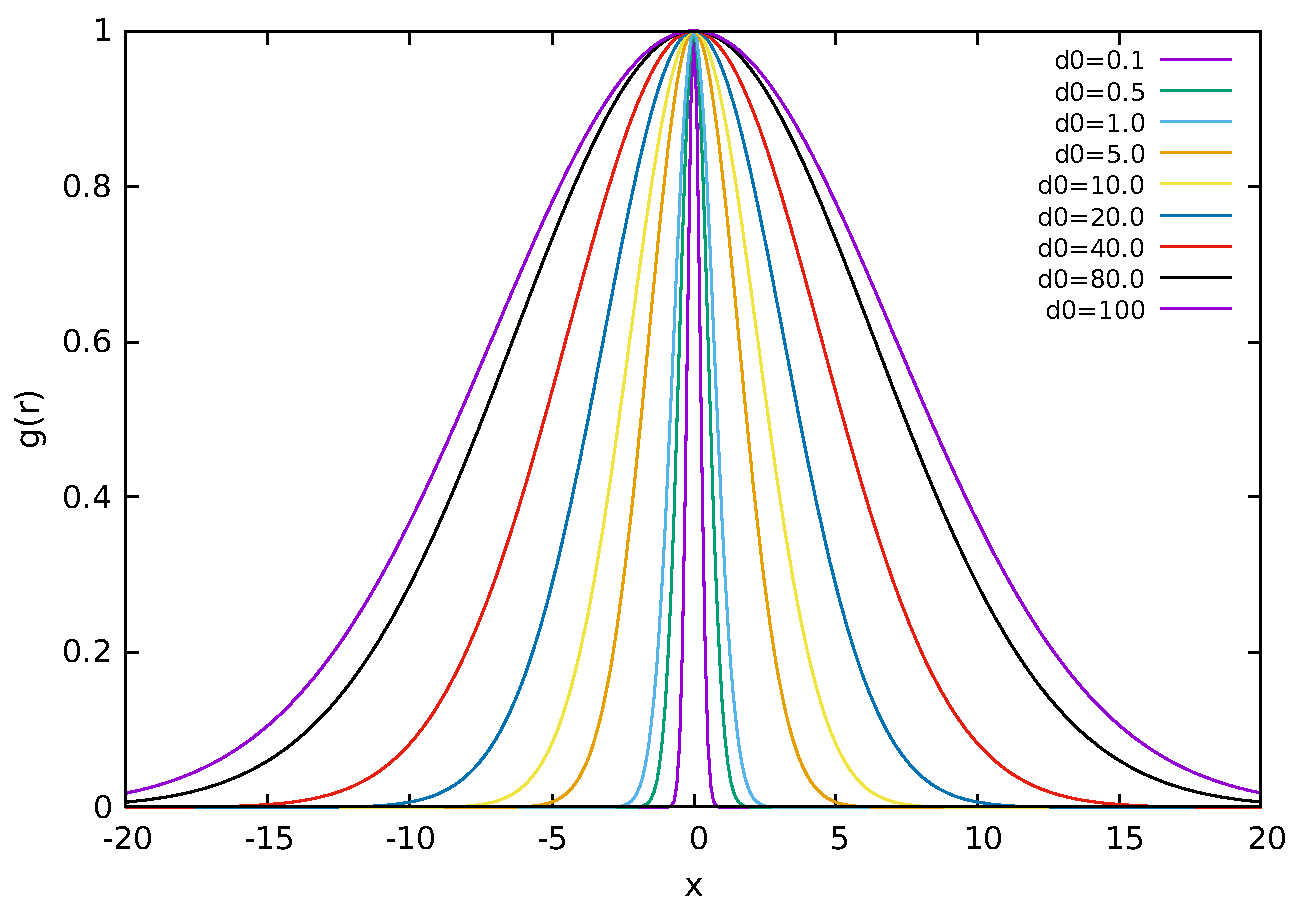
\includegraphics[width=0.7\textwidth, 
    height=0.41\textwidth, scale=1]{Gaussian_RBF.pdf}
    \caption{$g(χ)$ RBF shape for various $d_{0}$ values 
    when $χ \in [-20, 20]$}
\end{figure}

EASY built-in RBFs are described by equation \ref{RBF_equation}. In 
SMT,  
\newpage
%--------------------------------------------------------

\chapter{Numerical Cases}
The efficacy of the selected metamodels is tested on a pair 
of pseudo-engineering optimization problems. The study involves 
a comparison between MAEA-based optimization using the 
metamodels selected in this thesis, MAEAs using EASY built-in 
RBF models and plain EAs. The entirety of the evaluations are 
performed on the multi-processor platform of the PCOpt/NTUA 
that consists of 3 clusters with combined computational power 
of 62 Teraflop. The outcome of the evaluation will provide 
important feedback regarding the potential of the selected 
surrogate models.
\vfill

\section{Welded Beam Design}
The first case is a welded beam design \cite{welded beam}, 
a SOO optimization problem where a beam is welded onto a 
rigid body (see figure \ref{fig:welded_beam_image}). In this 
optimization case, the dimensions of the beam and the weld are 
modified in order for the overall construction cost to be minimized 
subject to constraints on shear stress, bending stress, buckling 
load and the end deflection. The design variables to be modified 
are four, i.e. the thickness of the welds $h$, the length of the 
welds $l$, the height of the beam $t$ and the width of the beam 
$b$. Consequently, the vector of design variables assumes the 
following form $\vec{β} = \left( β_{1}, β_{2}, β_{3}, β_{4} \right) 
= \left( h, l, t, b \right) \in \mathbb{R}^{4}$.
\begin{figure}[h!]
\centering
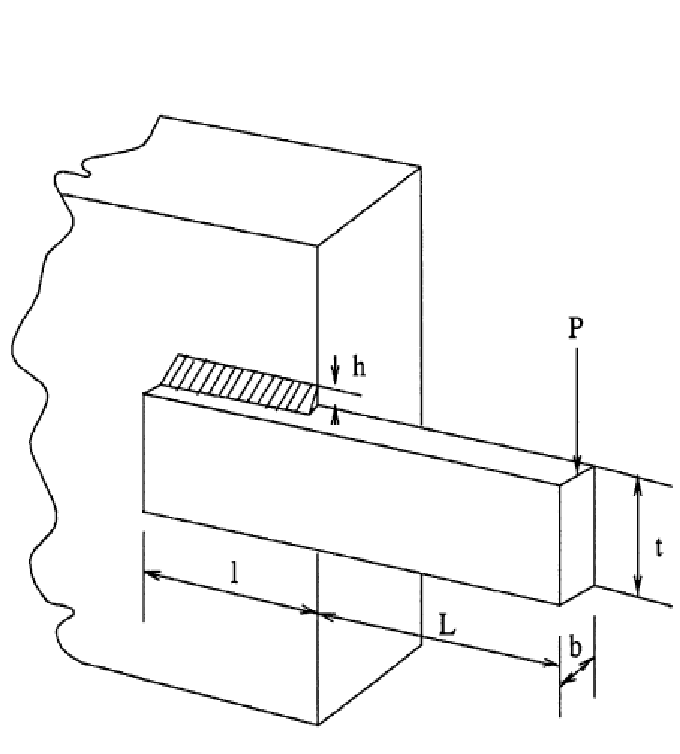
\includegraphics[width=0.55\textwidth, height=0.4\textwidth]
{welded_beam}   
\caption{Welded beam design} 
\label{fig:welded_beam_image}
\end{figure}


\newpage
%-----------------------------------------------------------

The beam is made of 1010 steel and must be supported by an 
upper and a lower weld when a constant load $P = 6000$ lb is 
applied at distance $L = 14 \hspace{2mm} in$ from the rigid 
body. The fabrication cost of the welds is given by the 
equation:
$$ f_{w} = (c_{1} + c_{2})h^{2}l$$
\\[-0.4cm]
where $c_{1}$ is the cost per unit volume of the weld 
material, $c_{2}$ the labour cost per unit weld volume and 
$V_{w} = h^{2}l$ the volume of the weld material.

The fabrication cost of the beam is proportional to the 
amount of material in the beam:
$$ f_{b} = c_{3}tb(L + l) = c_{3}tb(14.0 + l)$$
\\[-0.3cm]
where $c_{3}$ is the cost per unit volume of the beam and 
$V_{b} = tb(L + l)$ the respective volume. The construction 
costs $c_{1}, c_{2}, c_{3}$ have been estimated:
\begin{itemize}
\item For the welds: \\ 
\( c_{1} = 0.10471 \hspace{2mm} \dfrac{\$}{in^{3}} \) and 
\( c_{2} = 1 \hspace{2mm} \dfrac{\$}{in^{3}} \)
\item For the beam: \\ 
\( c_{3} = 0.04811 \hspace{2mm} \dfrac{\$}{in^{3}} \)
\end{itemize} 
\vspace{2mm}
The overall fabrication cost can be written as:
\begin{equation}
f_{tot} = f_{w} + f_{b} = 1.10471h^{2}l + 0.04811tb(14.0 + l)
\end{equation}

The stress states that describe the optimization case are 
subsequently defined and will serve as the imposed 
constraints. The first is the shear stress of the welds that must 
not exceed the maximum allowable shear stress of the material 
$τ_{max} \leq 13600$ psi. The shear stress of the welds is defined 
as such:
\begin{equation}\label{welded_con1}
τ = \sqrt{ τ_{p}^{2} + 2τ_{p}τ_{t}cosθ + τ_{t}^{2} } 
\xrightarrow{cosθ = l/2R} 
\sqrt{ τ_{p}^{2} + \dfrac{lτ_{p}τ_{t} }{R} + τ_{t}^{2} } 
\end{equation}
\\[-0.2cm]
where $R$ is the distance from the center of the 
cross-section of the beam, $τ_{p}$ the primary stress of the 
weld throat and $τ_{t}$ the torsional stress developed on the 
beam due to the torque $M$ developed by the applied load $P$ 
at its end. The equations describing the aforementioned 
static mechanical phenomena are the following:
\begin{equation}
\begin{split}
& R = \sqrt{\dfrac{l^{\hspace{0.5mm}2}}{4} + \left( 
\dfrac{h + t}{2} \right)^{2} } 
\\[0.2cm] &
τ_{p} = \dfrac{P}{\sqrt{2}hl} = \dfrac{6000}{\sqrt{2}hl}
\\[0.3cm] &
τ_{t} = \dfrac{MR}{J}
\\ & 
M = P\left(L + \dfrac{l}{2} \right) = 6000 \left(14.0 + 
\dfrac{l}{2} \right)
\end{split}
\end{equation}

\newpage
%-------------------------------------------------------

In torsional stress equation, the variable $J$ is the polar 
moment of inertia of the weld:
$$ J = 2\sqrt{2}hl \left[ \dfrac{l^{\hspace{0.5mm}2}}{12} + 
\left( \dfrac{h + t}{2} \right)^{2}  \right]$$ 
\\
The second stress that affects the quality of the design is 
the normal bending stress of the beam that must not exceed 
the maximum yield strength of the material $σ_{max} \leq 
30000$ psi and is equal to:

\begin{equation}\label{welded_con2}
σ = \dfrac{6PL}{bt^{2}} = \dfrac{504000}{bt^{2}}
\end{equation} 
\\[-0.1cm]
The deflection at the end of the beam is the next constraint 
that must be incorporated into the optimization of the welded 
beam. The deflection of a cantilever beam of length 
$L = 14 \hspace{2mm} in$ must not exceed $δ_{max} \leq 
0.25 \hspace{2mm} in$ and is calculated as such:

\begin{equation}\label{welded_con4}
δ = \dfrac{4PL^{3}}{Ebt^{3}} = \dfrac{2.1952}{bt^{3}}
\end{equation} 
\\[-0.2cm]
where $E$ is the Young's modulus; for 1010 steel is equal
to $30 \times 10^{6}$ psi.

Additionally, the structural integrity of the beam requires 
that the buckling load in the vertical direction must be
greater than the applied load $P = 6000$ psi. The critical 
buckling load of the beam is calculated as such:

\begin{equation}\label{welded_con5}
P_{c} = \dfrac{4.013 \sqrt{\dfrac{EGt^{2}b^{6}}{36}}}{L^{2}}
\left( 1 - \dfrac{t}{2L} \sqrt{\dfrac{E}{4G}} \right)
\end{equation}
\\
where $G$ is shearing modulus; for steel 1010 is equal to 
$G = 12 \times 10^{6}$ psi. 

It is evident that the thickness of the welds $h$ should not
exceed the width of the beam and therefore the last imposed
constraint is $h \leq b$. Consequently, the optimization of 
the welded beam design requires the minimization of a single 
objective, i.e. the fabrication cost of the structural design,
in the 4-dimensional space formed by the design 
variables $\vec{β} = \left( β_{1}, β_{2}, β_{3}, β_{4} \right)\!
= \!\left( h, l, t, b \right) \in \mathbb{R}^{4}$ and bounded 
by the 5 imposed constraints. 

\begin{equation}
\begin{split}
min \hspace{2mm} & f(\vec{β}) = 1.10471β_{1}^{2}β_{2} + 
0.04811β_{3}β_{4}(14.0 + β_{2}) 
\\[0.2cm] 
\text{subject to} \hspace{2mm} & c_{1}(\vec{β}) = 
τ(\vec{β}) - τ_{max} \leq 0 
\\ &
c_{2}(\vec{β}) = σ(\vec{β}) - σ_{max} \leq 0
\\ &
c_{3}(\vec{β}) = β_{1} - β_{4} \leq 0
\\ &
c_{4}(\vec{β}) = δ(\vec{β}) - δ_{max} \leq 0
\\ &
c_{5}(\vec{β}) = P - P_{c}(\vec{β}) \leq 0
\end{split}
\end{equation}
\\
where the bounds of each design variable are $0.125 \leq 
β_{1} \leq 10.0$, $0.1 \leq β_{2} \leq 10.0$, $0.1 \leq β_{3} 
\leq 10.0$ and $0.1 \leq β_{4} \leq 10.0$. The formulas that 
describe $τ(\vec{β})$, $σ(\vec{β})$, $δ(\vec{β})$ and 
$P_{c}(\vec{β})$ can be found in equations \ref{welded_con1}, 
\ref{welded_con2}, \ref{welded_con4} and \ref{welded_con5}, 
respectively.

\newpage

%-----------------------------------------------------------
%-------EAs----------
%------------------------------------------------------
\begin{itemize}
\item \textbf{Optimization using EAs}
\end{itemize}

First, the welded beam design is optimized using plain EAs 
that utilise the problem-specific evaluation model. The 
optimization is performed using EASY software in order to 
identify the most suitable values for the parameters of the 
evolution, e.g. offspring and parents population size, mutation 
probability and crossover scheme. The evolution parameters 
identified via the use of EAs are later used to facilitate the 
evolution in MAEA-based optimization. The number of offspring and 
parent population is set to $(μ,λ) = (20, 60)$ where 4 parents are 
combined to create a single offspring with one-point crossover. 
Gray binary encoding is used and 15 bits are assigned to each 
design variable. The optimization phase terminates after 27000 
PSM evaluations have been performed and is repeated for 5 
randomly initialised offspring populations $P_{λ}^{0}$ via the use 
of a Random Number Generator (RNG). The results are presented in 
table \ref{table:EAs_welded_beam} and in figure 
\ref{fig:EAs_welded_beam}.

\begin{table}[h!]
\centering
%\rowcolors{2}{gray!30!}{white!50!gray!10}
\scalebox{0.85}{%
\begin{tabular}[c]{ |p{1cm}||p{1.5cm}|p{1.2cm}|p{1.2cm}|
p{1.8cm}|p{1.6cm}|}
\toprule
\multicolumn{6}{|c|}{\cellcolor{gray!30!} 
\textbf{Welded beam case}} \\
\midrule 
& $(μ,λ)$ \textbf{population} & \textbf{Best} & 
\textbf{Worst} & \textbf{Average} & \textbf{Average PSM eval.} \\
\hline
\textbf{EAs} & (20, 60) & 2.38 & 2.49 & 2.43 & 27000 \\
\bottomrule
\end{tabular}%
}
\caption{Optimization of welded beam design using EAs}
\label{table:EAs_welded_beam}
\end{table}

\begin{figure}[h!]
\centering
	\begin{subfigure}[b]{0.49\textwidth}
    \centering
    \caption{Comparison between the convergence histories of 5 
    different $λ$ initializations}
    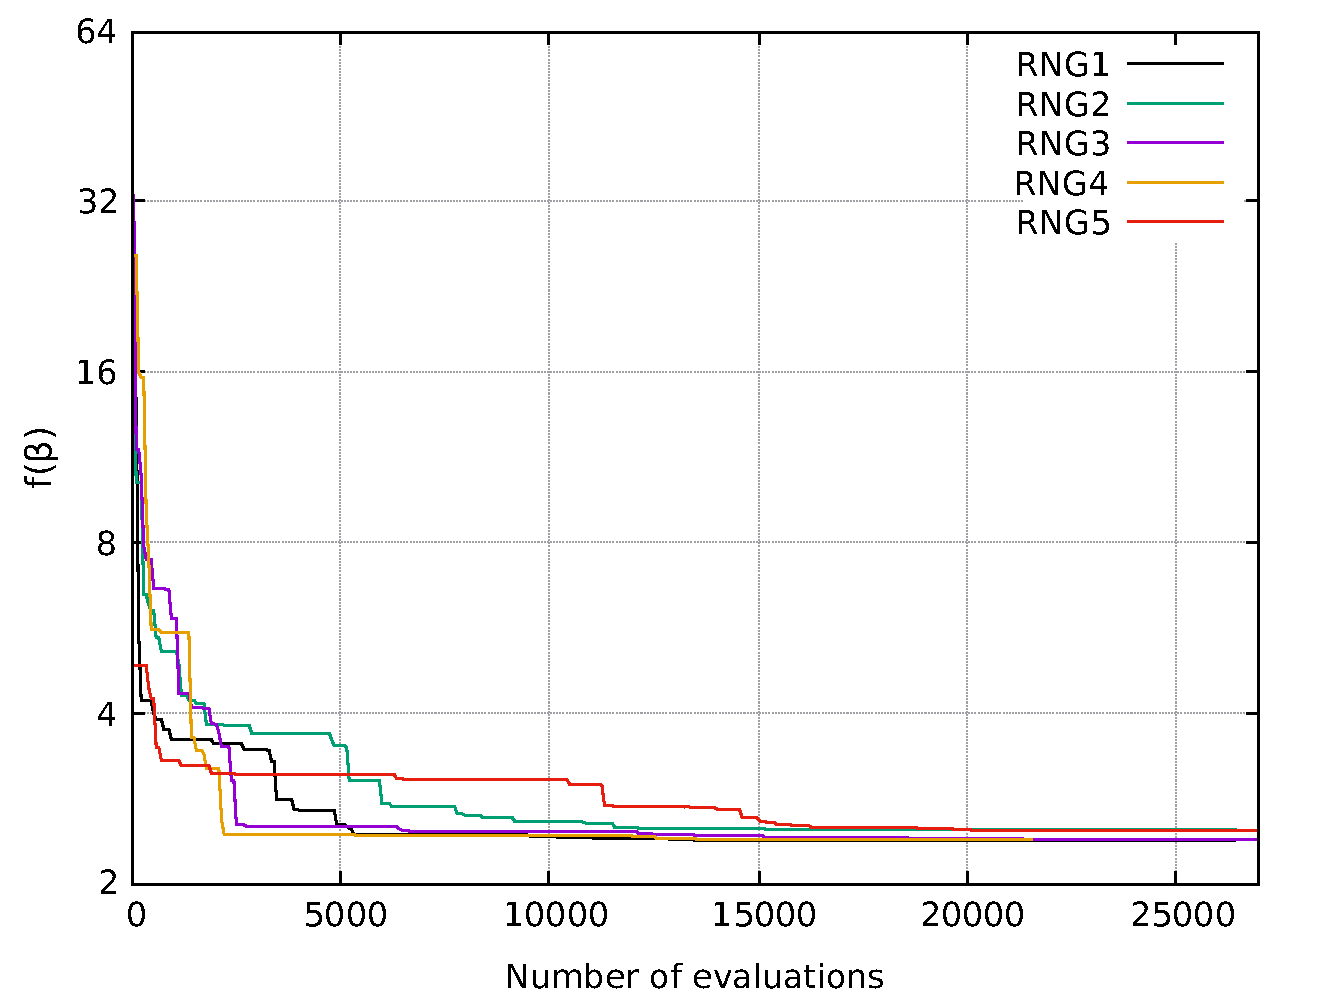
\includegraphics[width=\textwidth, height=0.28\textheight, 
    scale=1.0]{welded_beam_ea.pdf}    
    \end{subfigure}
    \hfill
    \begin{subfigure}[b]{0.49\textwidth}
    \centering
    \caption{Convergence history of the optimal run}
    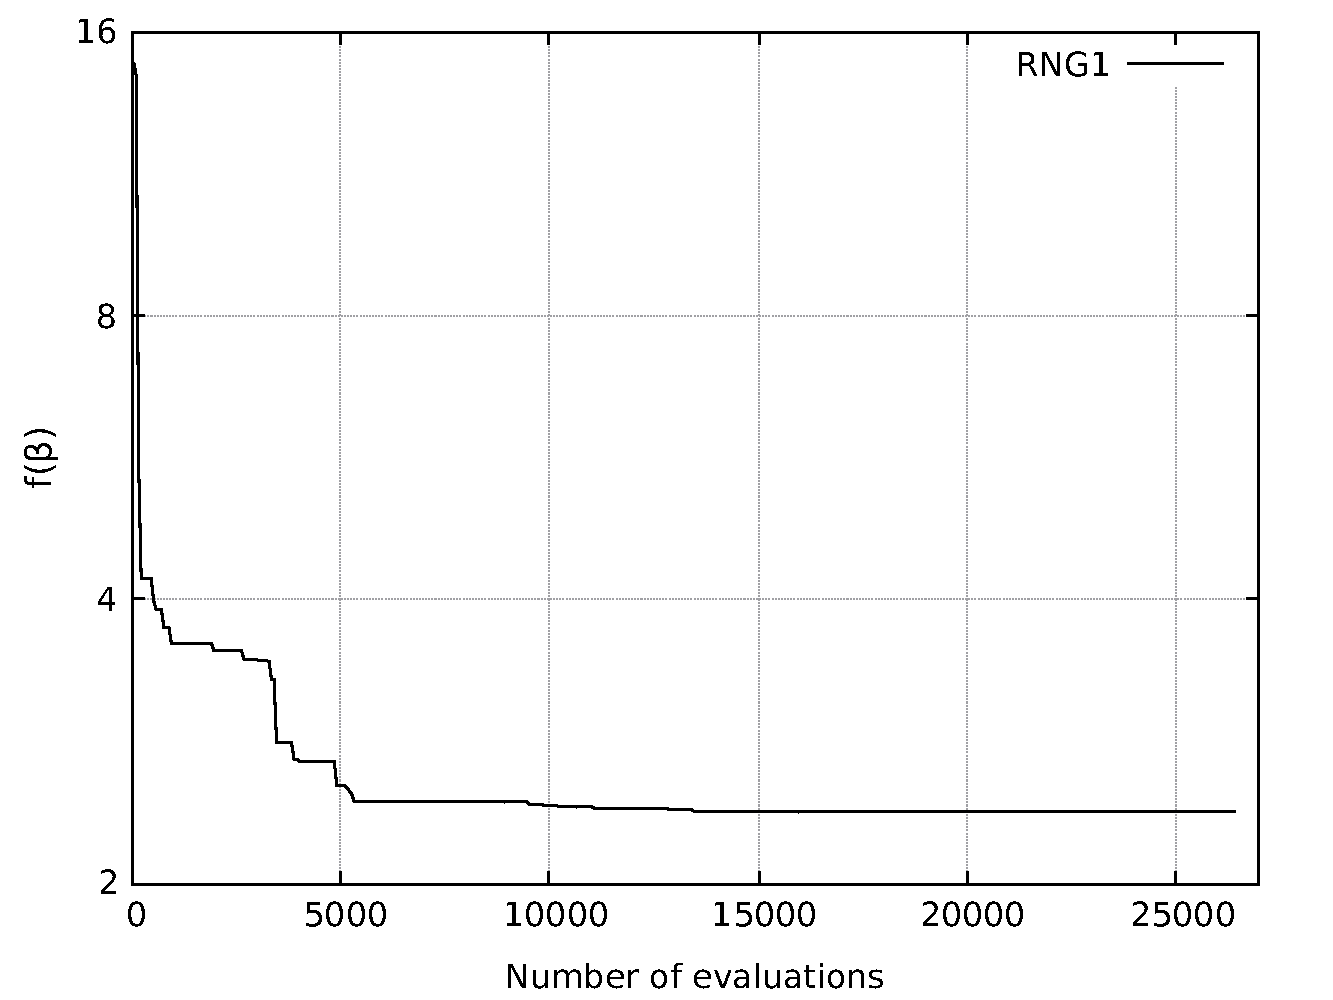
\includegraphics[width=\textwidth, height=0.28\textheight, 
    scale=1.0]{welded_beam_ea_best.pdf}    
    \end{subfigure}  
\caption{Convergence history of welded beam optimization case 
using EAs} 
\label{fig:EAs_welded_beam}
\end{figure}

The design variable vector that minimizes the construction
cost of the welded beam using plain EAs initialized via RNG1 is 
$\vec{β} = [0.244, 6.194,$ $8.329, 0.244]$. 

\newpage

%---------------------------------------------------------
%---------Off line------------
%----------------------------------------------------------

\begin{itemize}
\item \textbf{Optimization using MAEAs with off-line trained 
metamodels}
\end{itemize}

In MAEAs using off-line trained metamodels, both the 
objective $\mathbf{F}(\vec{β})$ and the imposed constraints 
$\mathbf{C}(\vec{β}) = [\vec{c}_{1}, \vec{c}_{2}, \hdots, 
\vec{c}_{n_{t}}]^{T}$, where $\vec{c}_{i} = [c_{i,1},
 c_{i,2}, \hdots, c_{i,n_{c}}]$, are approximated using 
surrogate models. Specifically, a global metamodel is built 
on the single objective and $n_{c}$ unique metamodels on each 
imposed constraint. In this case, the objective function is 
approximated by a KPLS model, while each constraint is 
approximated via the use of Kriging model; responsible for the 
construction of the aforementioned metamodels is SMT software. 
Alternatively, a single surrogate model can be trained to 
approximate the entirety of the constraints but this approach 
resulted in a poorly trained surrogate model. However, even the 
first approach resulted in surrogate models with poor overall 
fitting, especially when approximating a function with design 
variables in the denominator that tend to zero. To solve this 
issue an approach is proposed where constraints with denominators 
that tend to 0 are reduced to polynomials. Let the original 
approach of unmodified constraints be case 1 and let the modified 
approach be case 2, then:

\begin{equation}
\begin{split}
& c_{1}(\vec{β}) =  \sqrt{ τ_{p}^{2} + 
\dfrac{τ_{p}τ_{t}β_{2}}{R} + τ_{t}^{2} } - τ_{max} \leq 0
\Rightarrow \hspace{2mm}
τ_{p}^{2} + \dfrac{τ_{p}τ_{t}β_{2}}{R} + τ_{t}^{2} \leq 
τ_{max}^{2} \xrightarrow{R > 0}
\\[0.3cm] &
τ_{p}τ_{t}β_{2} \leq - R \left[ τ_{p}^{2} + τ_{t}^{2} - τ_{max}
^{2} \right] \xrightarrow{τ_{p}τ_{t}β_{2} > 0}\hspace{1mm}
c_{1}(\vec{β})_{new} = \dfrac{R \left[τ_{p}^{2} + τ_{t}^{2} -
τ_{max}^{2} \right] }{τ_{p}τ_{t}β_{2}}  - 1 \leq 0
\end{split}
\end{equation}
\\[-0.4cm]
\begin{equation}\label{con2_mod}
c_{2}(\vec{β}) = \dfrac{6PL}{β_{4}β_{3}^{2}} -σ_{max} \leq 0 
\xrightarrow{β_{3}, β_{4} > 0} c_{2}(\vec{β})_{new} = 
6PL - σ_{max}β_{4}β_{3}^{2} \leq 0
\end{equation}
\\[-0.2cm]
\begin{equation}\label{con4_mod}
c_{4}(\vec{β}) = \dfrac{4PL^{3}}{Eβ_{4}β_{3}^{3}} - δ_{max} 
\leq 0 \xrightarrow{β_{3}, β_{4} > 0} c_{4}(\vec{β})_{new} = 
4PL^{3} - δ_{max}Eβ_{4}β_{3}^{3} \leq 0
\end{equation}
\vspace{-2mm}

\begin{figure}[h!]
\centering
\begin{subfigure}[b]{0.49\textwidth}
    \centering
    \caption{Case 1: Comparison between $c_{4}(\vec{β})$ and 
    $\widehat{c}_{4}(\vec{β})$} 
    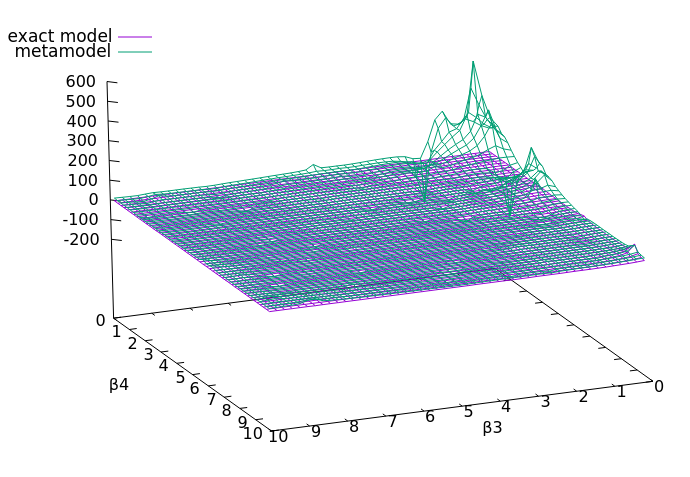
\includegraphics[width=\textwidth, height=0.75\textwidth, 
    scale=1]{con4_welded_beam_before.png}    
    \end{subfigure}
    \hfill
    \begin{subfigure}[b]{0.49\textwidth}
    \centering 
    \caption{Case 2: Comparison between $c_{4}(\vec{β})$ and 
    $\widehat{c}_{4}(\vec{β})$}
    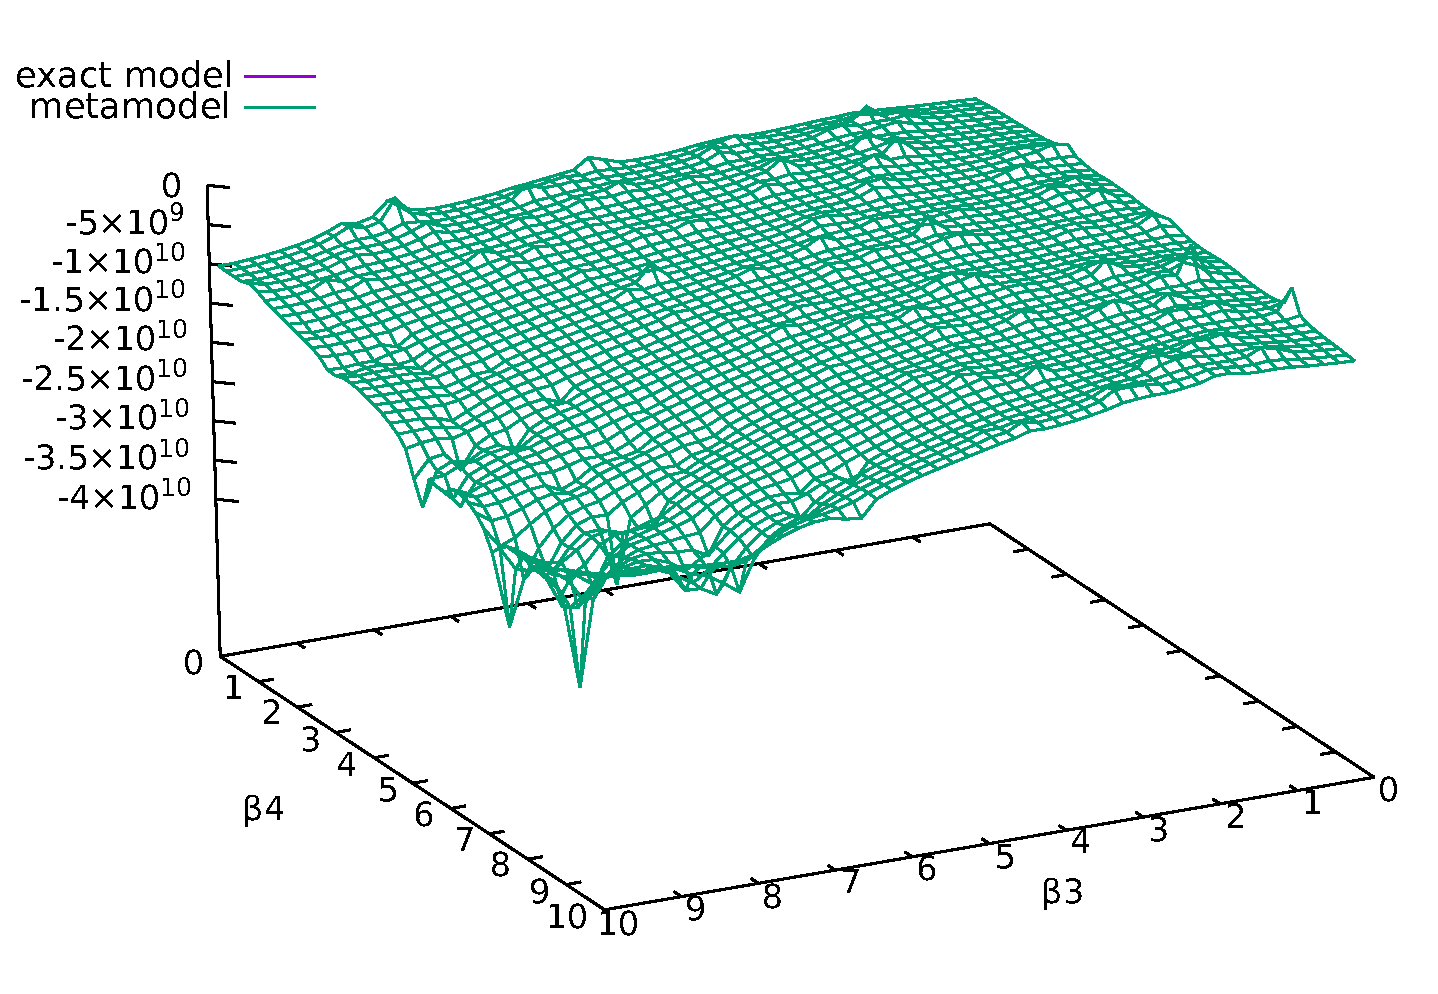
\includegraphics[width=\textwidth, height=0.75\textwidth, 
     scale=1]{con4_welded_beam_after.pdf} 
    \end{subfigure}
\caption{Error of the metamodel when approximating the original 
NRMSE = 1.206111 (left) and the modified NRMSE = $1.182408 \!
\cdot \! 10^{-6}$ (right) equation $c_{4}(\vec{β})$ using an 
LHD composed of $n_{t} = 240$ training patterns}
\label{fig:mod_c4} 
\end{figure}

\newpage
%----------------------------------------------------------


\begin{figure}[h!]
\centering
	\begin{subfigure}[b]{0.49\textwidth}
    \centering
    \caption{Case 1: $c_{2}(\vec{β})$ function}
    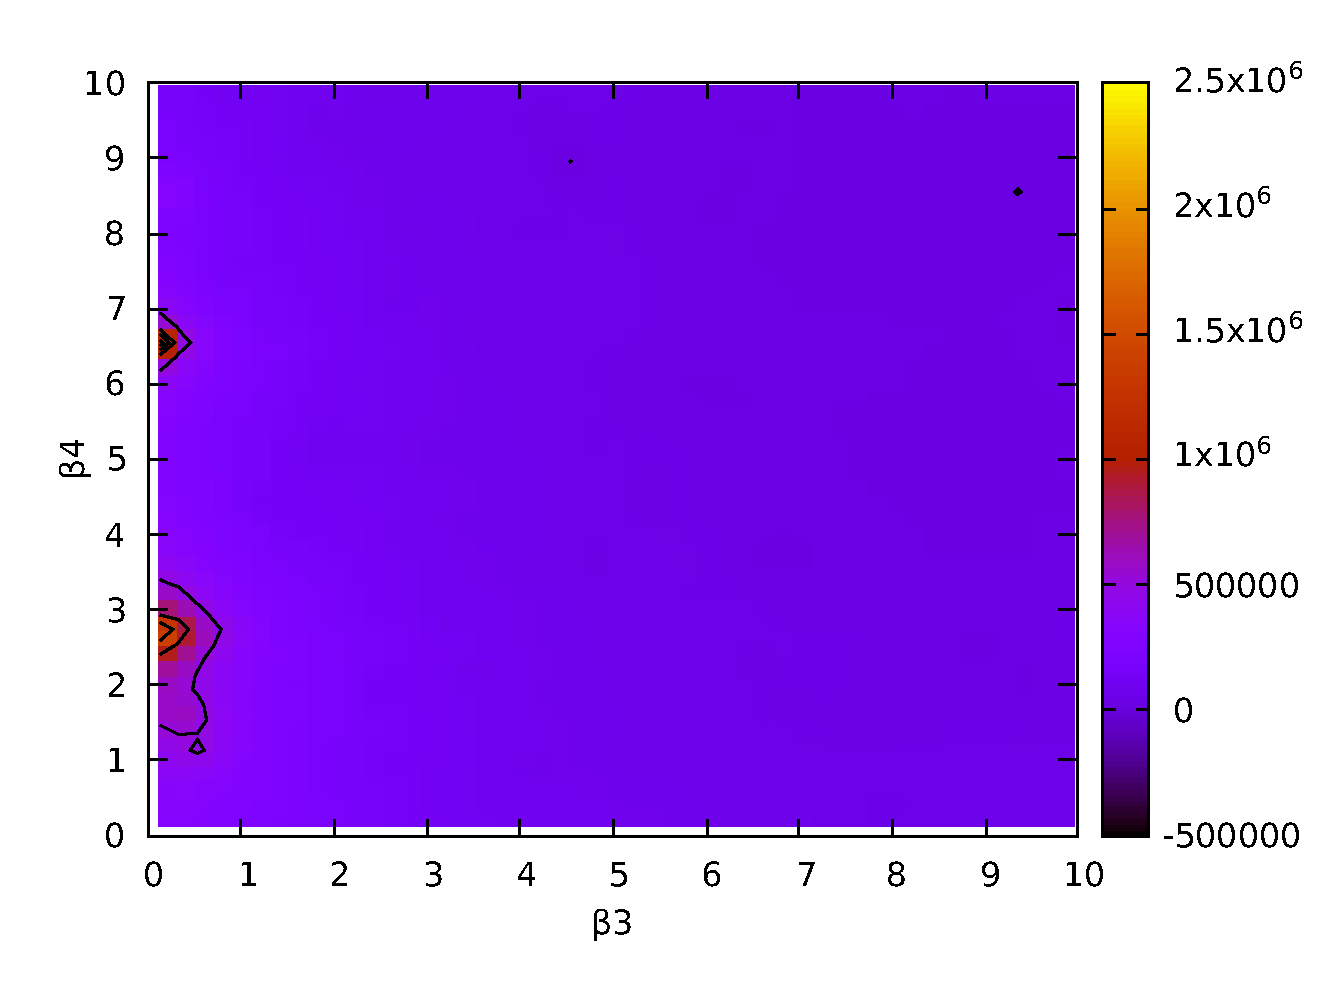
\includegraphics[width=\textwidth, height=0.9\textwidth, 
    scale=1]{con2_welded_beam_contour_before.pdf}    
    \end{subfigure}
    \hfill
    \begin{subfigure}[b]{0.49\textwidth}
    \centering 
    \caption{Case 2: $c_{2}(\vec{β})$ function}
    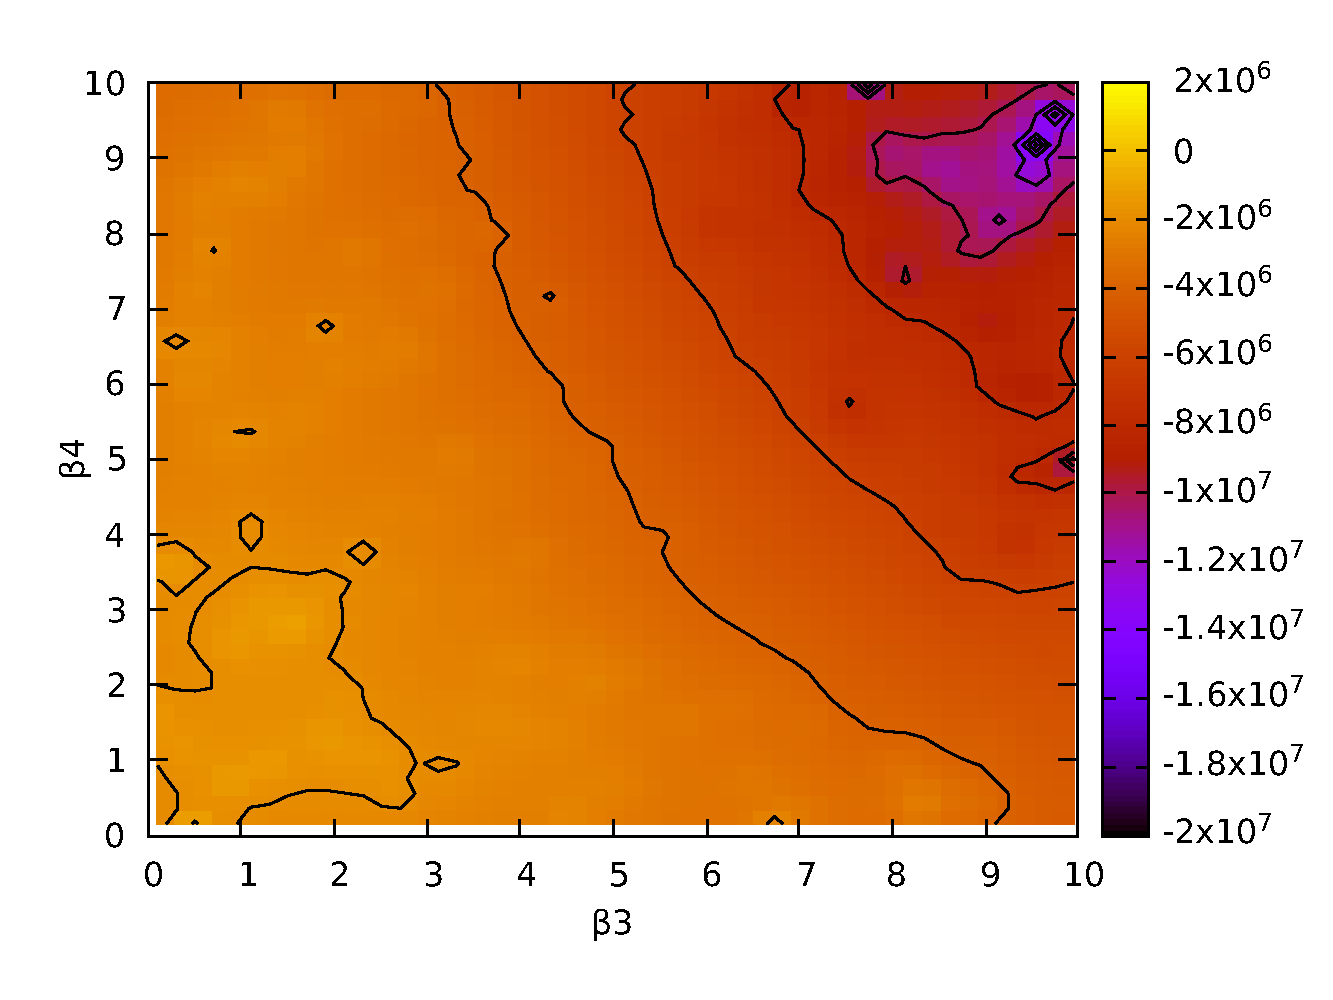
\includegraphics[width=\textwidth, height=0.9\textwidth, 
     scale=1]{con2_welded_beam_contour_after1.pdf} 
    \end{subfigure}
    \hfill
    \begin{subfigure}[b]{0.49\textwidth}
    \centering
    \caption{Case 1: Prediction $\widehat{c}_{2}(\vec{β})$ 
    function}
    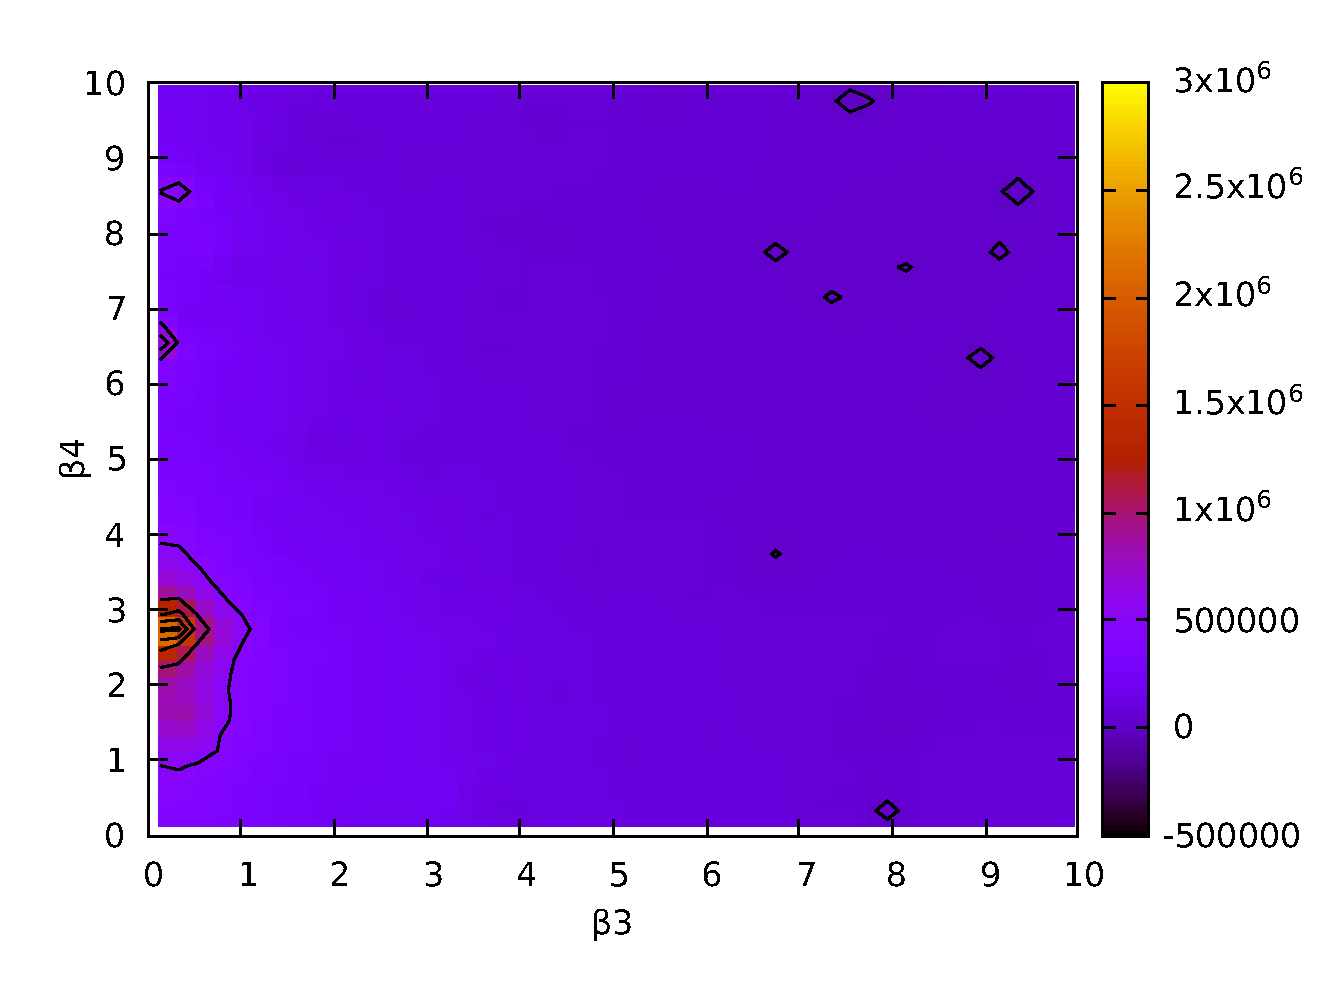
\includegraphics[width=\textwidth, height=0.9\textwidth, 
    scale=1]{con2_welded_beam_contour_before_metamodel.pdf}    
    \end{subfigure}
    \hfill
    \begin{subfigure}[b]{0.49\textwidth}
    \centering 
    \caption{Case 2: Prediction $\widehat{c}_{2}(\vec{β})$}
    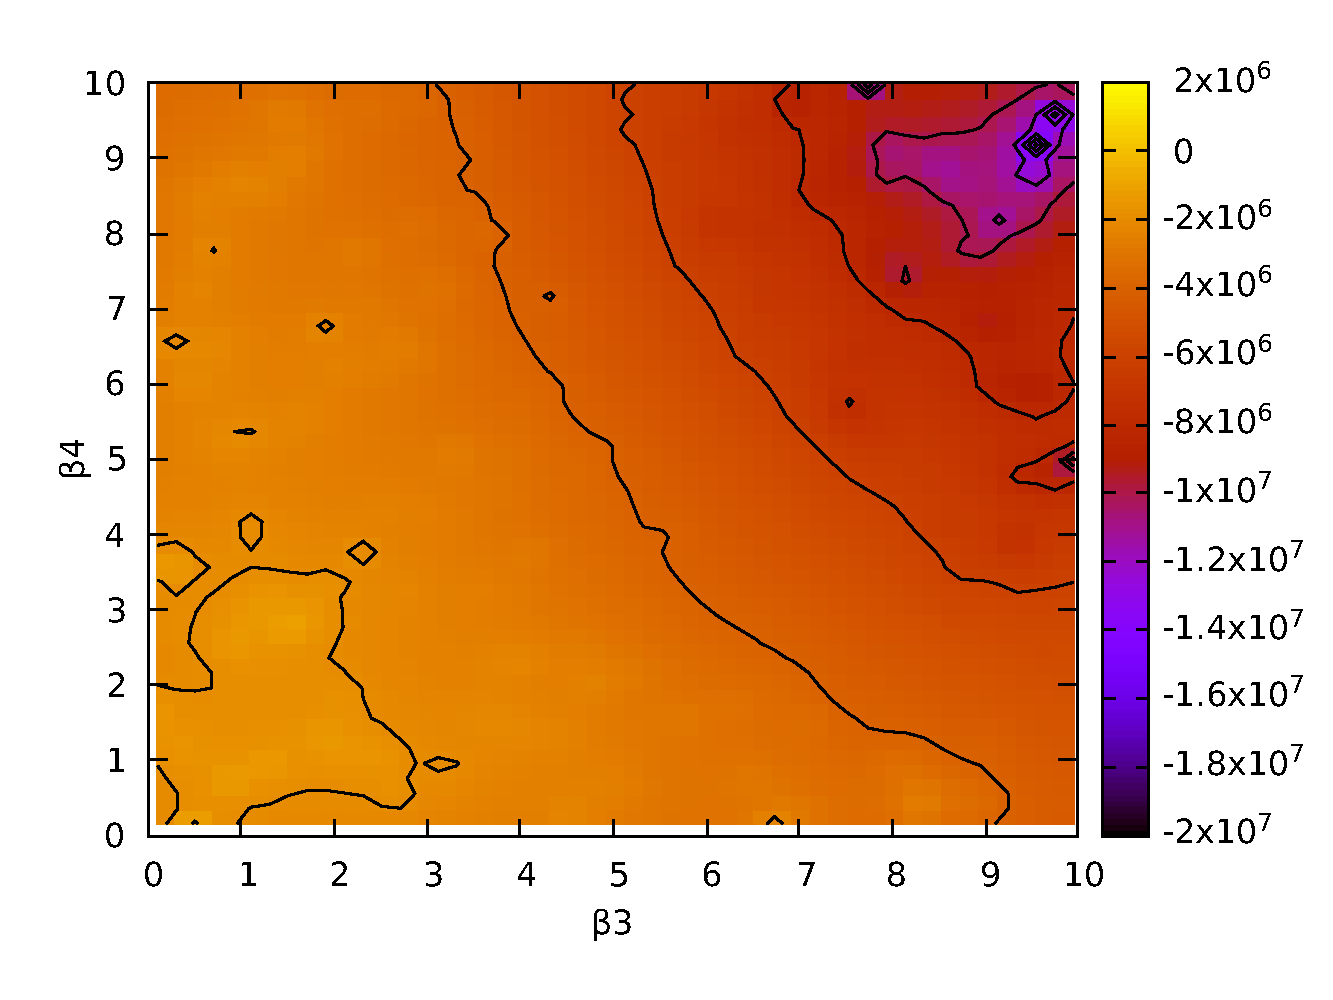
\includegraphics[width=\textwidth, height=0.9\textwidth, 
     scale=1]{con2_welded_beam_contour_after1.pdf} 
    \end{subfigure}
\caption{Contour projections to 2D plane for the original 
(left) and modified (right) function of the 2nd constraint}
\label{fig:mod_c2} 
\end{figure}

In both figures, i.e. \ref{fig:mod_c4} and \ref{fig:mod_c2},
the visualization of the constraint function justifies the 
initial assumption of underfitted metamodels built $\forall 
\vec{β} \in \mathbb{R}^n_{β}$ when $β_{1}, β_{4} \rightarrow 0$; 
such metamodels are trained in case 1. In case 2, the modification 
in constraints $c(\vec{β}_{1}), c(\vec{β}_{2})$ and $c(\vec{β}
_{4})$ results in a better model fitting, NRMSE = $1.182408 \!
\cdot \! 10^{-6}$ compared to NRMSE = 1.206111 of case 1. 
The minimization of the welded beam case that through 5 runs is 
presented in table \ref{table:offline_case2_welded_beam}, where a 
maximum of 5000 evaluations per cycle are performed using MAEAs 
with off-line trained metamodels:

\begin{table}[h!]
\centering
%\rowcolors{2}{gray!30!}{white!50!gray!10}
\scalebox{0.84}{%
\begin{tabular}[c]{ |p{3.4cm}||p{1.5cm}|p{1.2cm}|p{1.2cm}|
p{1.8cm}|p{2.3cm}|p{1.3cm}|}
\toprule
\multicolumn{7}{|c|}{\cellcolor{gray!30!} 
\textbf{Case 2}} \\
\midrule 
& $(μ,λ)$ \textbf{population} & \textbf{Best} & 
\textbf{Worst} & \textbf{Average} & \textbf{Avg. metamodel 
eval./cycle} & 
\textbf{Avg. cycles} \\
\hline
\textbf{MAEAs, off-line} & (20, 60) & 2.35 & 2.56 & 2.44 
& 3168 & 3 \\
\bottomrule
\end{tabular}%
}
\caption{Optimization of welded beam design using MAEAs with 
off-line training}
\label{table:offline_case2_welded_beam}
\end{table}

\newpage
%------------------------------------------------------------


The optimal candidate solution obtained via this method is 
$\vec{β} = [0.336, 5.067,$ $7.323, 0.338]$. The corresponding 
value of each constraint and objective is presented in table 
\ref{table:offline_case2_deviation_welded_beam}.

\begin{table}[h!]
\centering
%\rowcolors{2}{gray!30!}{white!50!gray!10}
\scalebox{0.83}{%
\begin{tabular}[c]{ |p{1.6cm}||p{2cm}p{1.8cm}p{1.4cm}
p{2.4cm}p{1.6cm}p{1cm}|}
\toprule
\rowcolor{gray!30!}
\textbf{Case 2} & $\mathbf{c_{1}}(\vec{\bm{β}})$ 
& $\mathbf{c_{2}}(\vec{\bm{β}})$ 
& $\mathbf{c_{3}}(\vec{\bm{β}})$ 
& $\mathbf{c_{4}}(\vec{\bm{β}})$ 
& $\mathbf{c_{5}}(\vec{\bm{β}})$ 
& $\mathbf{f}(\vec{\bm{β}})$ \\
\midrule
\textbf{MAEAs} & -0.412243 & -29020.84 & -0.019 
& -1065388211 & -276.80 & 2.35 \\
\textbf{PSM} & 1129.41 & -1633.52 & -0.019 
& -0.235446 & -261.95 & 2.35 \\
\bottomrule
\end{tabular}%
}
\caption{\textbf{C}, \textbf{F} responses to $\vec{β}$ found 
via MAEAs with off-line training in case 2}
\label{table:offline_case2_deviation_welded_beam}
\end{table}

MAEAs with off-line training utilizing the approach of modified 
constraints (case 2) converge in candidate solutions that 
violate the first constraint $c_{1}(\vec{β})$. In order to 
determine the extent to which the design space has changed, the 
aforementioned approach is implemented in plain EAs that 
utilize the modified problem-specific model, denoted by 
$\mathrm{PSM}^{'}$ for simplicity. If $\mathrm{PSM}^{'}$-based 
EAs converge to an optimal solution that lies in the design 
space of the original PSM, then the modification in 
constraints did not lead to a significant change in the design 
space of candidate solutions and the unsatisfactory solutions 
are contributed to metamodel-related flaws. EAs using 
$\mathrm{PSM}^{'}$ find the optimal solution $\vec{β} = 
[0.272, 4.300, 7.856, 0.272]$. The corresponding value of each 
constraint and objective is presented in table 
\ref{table:offline_case2_PSM_welded_beam}

\begin{table}[h!]
\centering
%\rowcolors{2}{gray!30!}{white!50!gray!10}
\scalebox{0.83}{%
\begin{tabular}[c]{ |p{1.4cm}||p{2cm}p{1.8cm}p{1.2cm}
p{2.2cm}p{1.8cm}p{1cm}|}
\toprule
\rowcolor{gray!30!}
\textbf{Case 2} & $\mathbf{c_{1}}(\vec{\bm{β}})$ 
& $\mathbf{c_{2}}(\vec{\bm{β}})$ 
& $\mathbf{c_{3}}(\vec{\bm{β}})$ 
& $\mathbf{c_{4}}(\vec{\bm{β}})$ 
& $\mathbf{c_{5}}(\vec{\bm{β}})$ 
& $\mathbf{f}(\vec{\bm{β}})$ \\
\midrule
$\mathbf{PSM^{'}}$ & -0.000037 & -273.75 & 0 
& -963206327 & -529.75 & 2.15 \\
\textbf{PSM} & 3445.91 & -16.286 & 0 
& -0.234001 & -529.75 & 2.15 \\
\bottomrule
\end{tabular}%
}
\caption{\textbf{C}, \textbf{F} responses to $\vec{β}$ found 
via EAs using the $\mathrm{PSM}^{'}$}
\label{table:offline_case2_PSM_welded_beam}
\end{table}

The implemented modifications seem to distort the design space
significantly, since the optimal solution results in a design 
with welds that undergo massive shear stress $c_{1}(\vec{β}) = 
17045.91$ psi. Consequently, optimal solutions found in 
case 2 do not satisfy the constraints imposed on the design 
space and result in a unsatisfactory welded beam design. 
However, metamodels trained off-line on the PSM do not 
converge to an optimal solution due to poor constraint model 
fitting. For this reason, a new approach is proposed, 
referred to as case 3, and is based on the observation that 
the entirety of optimal solutions found via the use both the 
$\mathrm{PSM}^{'}$ and metamodels trained on the $\mathrm{PSM}
^{'}$(case 2) do not satisfy the first constraint $c_{1}
(\vec{β})$. In case 3, therefore, constraints $c_{2}, c_{4}$ 
are modified according to equations \ref{con2_mod} and 
\ref{con4_mod}, respectively, and the corresponding problem-
specific model is denoted by $\mathrm{PSM}^{''}$. The 
implementation of EAs via the use of $\mathrm{PSM}^{''}$ 
yields the optimal solution $\vec{β} \!= \![0.279, 5.679, 7.698, 
0.284]$. The corresponding value of each constraint and objective 
is presented in table \ref{table:offline_case3_PSM_welded_beam}.

\begin{table}[h!]
\centering
%\rowcolors{2}{gray!30!}{white!50!gray!10}
\scalebox{0.83}{%
\begin{tabular}[c]{ |p{1.4cm}||p{1.6cm}p{1.6cm}p{1.4cm}
p{2.2cm}p{1.6cm}p{1cm}|}
\toprule
\rowcolor{gray!30!}
\textbf{Case 3} & $\mathbf{c_{1}}(\vec{\bm{β}})$ 
& $\mathbf{c_{2}}(\vec{\bm{β}})$ 
& $\mathbf{c_{3}}(\vec{\bm{β}})$ 
& $\mathbf{c_{4}}(\vec{\bm{β}})$ 
& $\mathbf{c_{5}}(\vec{\bm{β}})$ 
& $\mathbf{f}(\vec{\bm{β}})$ \\
\midrule
$\mathbf{PSM^{''}}$ & -13.645 & -355.91 & -0.004
& -904782848 & -2906.86 & 2.56 \\
\textbf{PSM} & -13.645 & -21.170 & -0.004
& -0.233038 & -2906.86 & 2.56 \\
\bottomrule
\end{tabular}%
}
\caption{\textbf{C}, \textbf{F} responses to $\vec{β}$ found 
via EAs using the $\mathrm{PSM}^{''}$}
\label{table:offline_case3_PSM_welded_beam}
\end{table}

\newpage
%-----------------------------------------------------------


Unlike previous approaches, $\mathrm{PSM}^{''}$-based EAs 
converge to an optimal solution that satisfies the entirety 
of the constraints imposed to the original model. Metamodels 
trained off-line on the $\mathrm{PSM}^{''}$ through 5 runs yield 
the outcome shown in table 
\ref{table:offline_case3_welded_beam}.

\begin{table}[h!]
\centering
%\rowcolors{2}{gray!30!}{white!50!gray!10}
\scalebox{0.85}{%
\begin{tabular}[c]{ |p{3.4cm}||p{1.5cm}|p{1.2cm}|p{1.2cm}|
p{1.8cm}|p{2.3cm}|p{1.3cm}|}
\toprule
\multicolumn{7}{|c|}{\cellcolor{gray!30!} 
\textbf{Case 3}} \\
\midrule 
& $(μ,λ)$ \textbf{population} & \textbf{Best} & 
\textbf{Worst} & \textbf{Average} 
& \textbf{Average metamodel eval./cycle} 
& \textbf{Avg. cycles} \\
\hline
\textbf{MAEAs, off-line} & (20, 60) & 2.90 & 3.55 & 3.12 
& 2883 & 8 \\
\bottomrule
\end{tabular}%
}
\caption{Optimization of welded beam design using MAEAs with 
off-line training}
\label{table:offline_case3_welded_beam}
\end{table}

The best solution $\vec{β} = [0.336, 5.067, 7.323, 0.338]$ obtained 
via MAEAs with off-line training, produces the constraint and 
objective function values shown in table 
\ref{table:offline_case3_deviation_welded_beam} when evaluated on 
the PSM.

\begin{table}[h!]
\centering
%\rowcolors{2}{gray!30!}{white!50!gray!10}
\scalebox{0.83}{%
\begin{tabular}[c]{ |p{1.6cm}||p{1.6cm}p{1.8cm}p{1.4cm}
p{2.2cm}p{1.6cm}p{1cm}|}
\toprule
\rowcolor{gray!30!}
\textbf{Case 3} & $\mathbf{c_{1}}(\vec{\bm{β}})$ 
& $\mathbf{c_{2}}(\vec{\bm{β}})$ 
& $\mathbf{c_{3}}(\vec{\bm{β}})$ 
& $\mathbf{c_{4}}(\vec{\bm{β}})$ 
& $\mathbf{c_{5}}(\vec{\bm{β}})$ 
& $\mathbf{f}(\vec{\bm{β}})$ \\
\midrule
\textbf{MAEAs} & -469.56 & -39385.13 & -0.002
& -928918812 & -8492.04 & 2.90 \\
\textbf{PSM} & -797.35 & -2194.43 & -0.002
& -0.233450 & -8522.98 & 2.90 \\
\bottomrule
\end{tabular}%
}
\caption{\textbf{C}, \textbf{F} responses to $\vec{β}$ found 
via MAEAs with off-line training in case 3}
\label{table:offline_case3_deviation_welded_beam}
\end{table}

Consequently, the MAEA-based optimization of the welded beam case 
is performed by utilizing metamodels built off-line exclusively on 
$\mathrm{PSM}^{''}$, since MAEAs with surrogate models trained 
off-line on $\mathrm{PSM}^{'}$ and PSM either converge to 
prohibited by the constraints solutions or they do not converge 
after performing 20 optimization cycles, respectively. The 
convergence histories of EAs using PSM, $\mathrm{PSM}^{'}$ and $
\mathrm{PSM}^{''}$ are subsequently presented in figure 
\ref{fig:convergence_PSMs} all EA methods are initialized with the 
same offspring population set $P_{λ}^{0}$ corresponding to best 
solution.

\begin{figure}[h!]
\centering
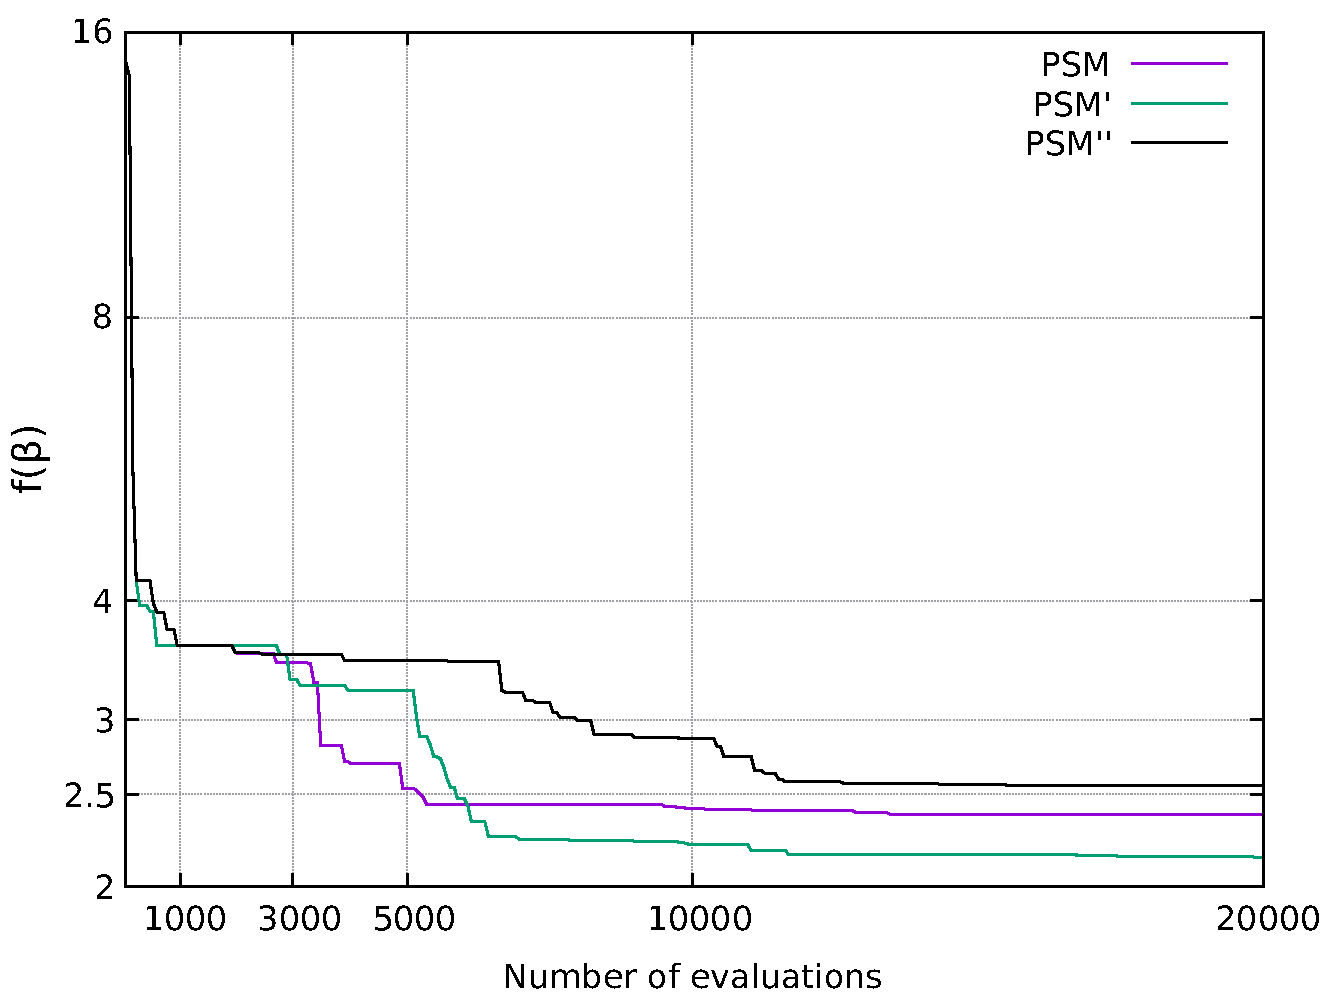
\includegraphics[width=0.6\textwidth]{EA_mod.pdf}   
\caption{Welded beam design. Comparison between the 
convergence history of EAs performing evaluations on the PSM, 
$\mathrm{PSM}^{'}$ and $\mathrm{PSM}^{''}$} 
\label{fig:convergence_PSMs}
\end{figure}

\newpage
%------------------------------------------------------------


The deviation between metamodel predicted values and evaluated 
ones, using the $\mathrm{PSM}^{''}$ of either objective function or 
some constraint, can be observed in figures 
\ref{fig:fitting_f_welded_beam}, 
\ref{fig:fitting_con1_2_welded_beam} and 
\ref{fig:fitting_con3_5_welded_beam}. The surrogate models are 
trained on $n_{t} \!= \!n_{doe} \!= \!240$ patterns $\mathbf{X}$ 
collected via the implementation of LHS that makes use of the ESE 
algorithm to construct an optimal space-filling design. At the end 
of each optimization loop, a new random design of $n_{new\_doe} \!= 
\!20$ points and 1 elite are added to the initial LHD. The 
optimization process converged after 10 cycles and, therefore, at 
the end of the optimization the metamodels are retrained on $n_{t} 
\!= \!n_{doe}^{'} \!= \!429$ patterns. Each individual $\vec{β} \!
\in \!P_{λ}^{0}$ selected in the first of the 5 total runs is used 
to validate both metamodels and calculate the NRMSE.
\vspace{-2mm}
\begin{figure}[h!]
\centering
    \begin{subfigure}[b]{0.45\textwidth}
    \centering
    \caption{Initial $f$, $\mathrm{NRMSE} \!= \!0.00000269$}
    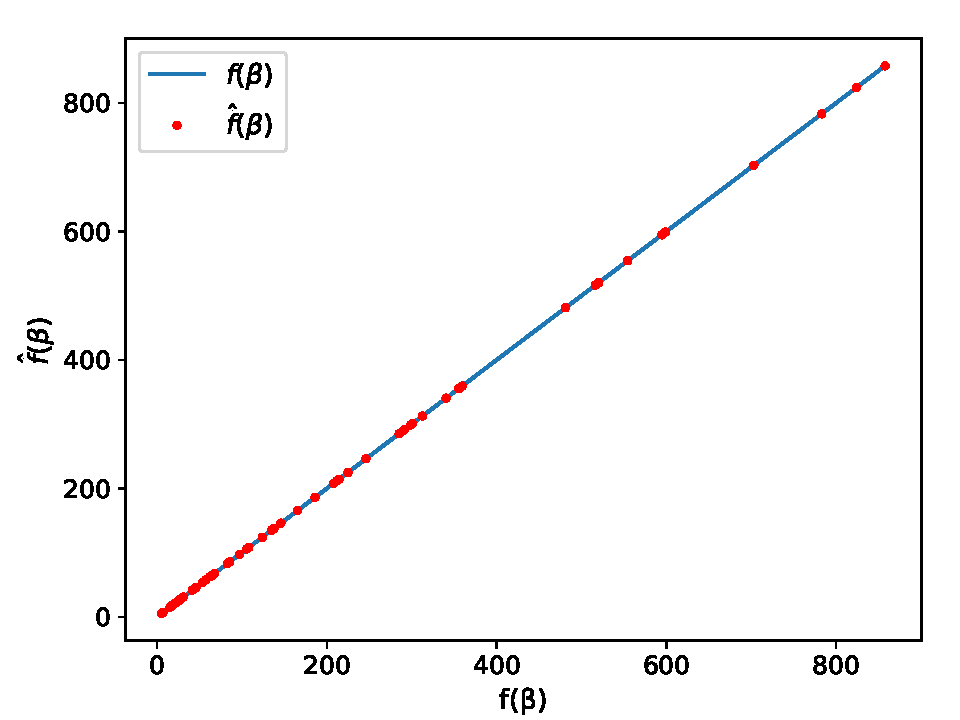
\includegraphics[width=\textwidth, height=0.6\textwidth, 
    scale=1]{welded_beam_f_fitness_start.pdf}    
    \end{subfigure}
    \hfill
    \begin{subfigure}[b]{0.45\textwidth}
    \centering
    \caption{Final $f$, $\mathrm{NRMSE} \!= \!0.00000042$}
    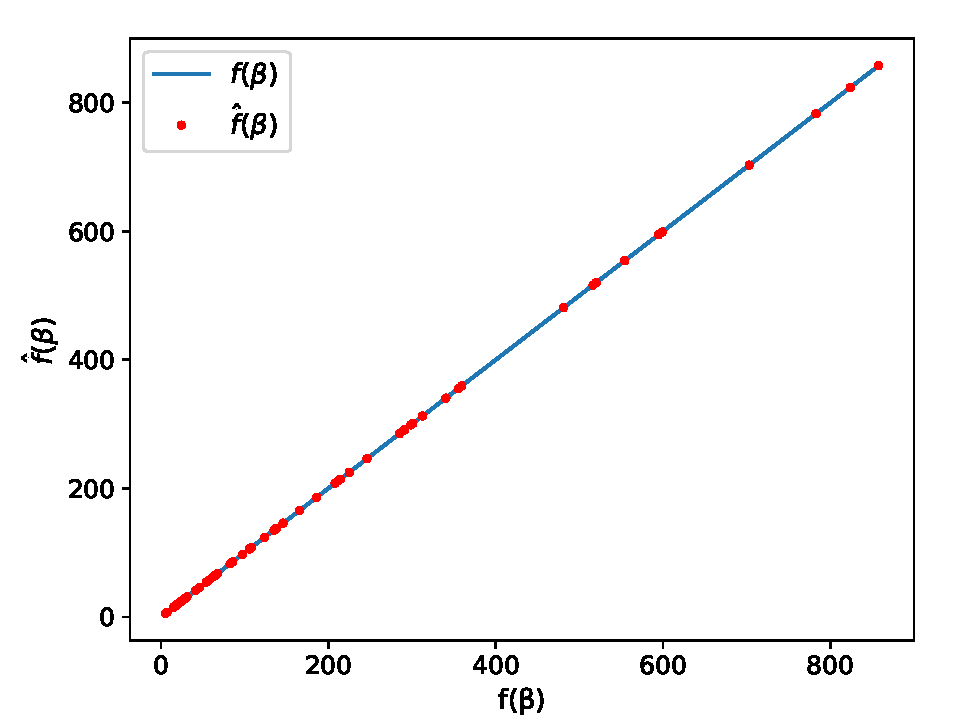
\includegraphics[width=\textwidth, height=0.6\textwidth, 
    scale=1]{welded_beam_f_fitness_end.pdf} 
    \end{subfigure}
    \caption{Case 3, welded beam case with RNG1. Deviation between 
    exact $\mathrm{PSM}^{''}$ values of the objective function 
    $\vec{f}(\vec{β})$ and KPLS predictions $\hat{\vec{f}}(\vec{β})
    $. The initial KPLS model is trained on $n_{doe} \!= \!240$ and 
    the final on $n_{doe}^{'} \!= \!429$ training patterns.}
    \label{fig:fitting_f_welded_beam}
\end{figure}
\vspace{-4mm}
\begin{figure}[h!]
\centering
    \begin{subfigure}[b]{0.45\textwidth}
    \centering
    \caption{Initial $c_{1}$, $\mathrm{NRMSE} \!= \!0.7773964$}
    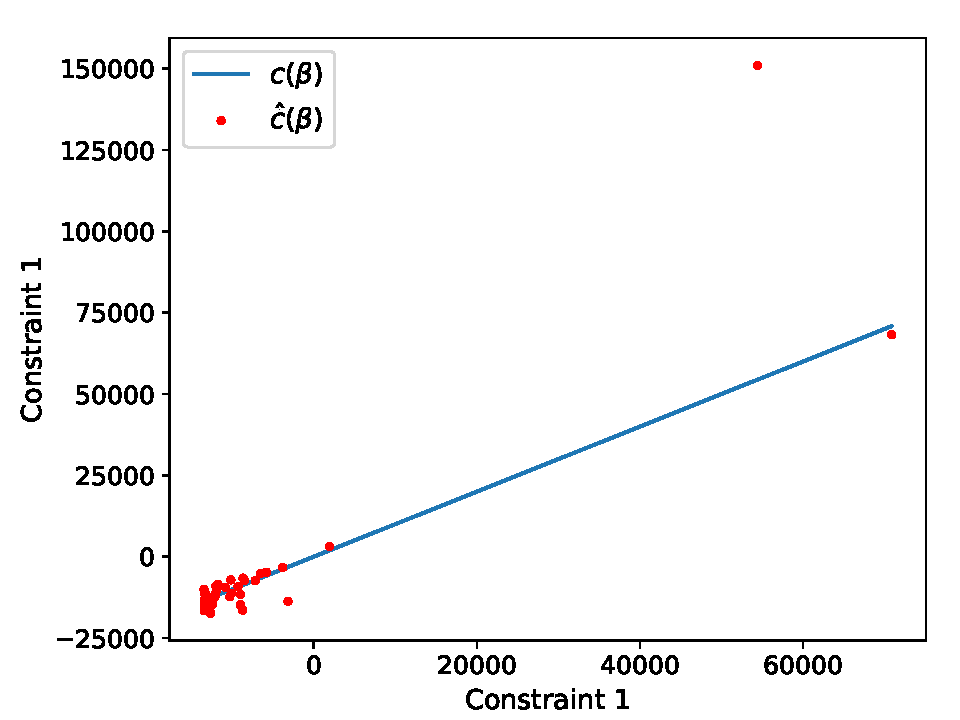
\includegraphics[width=\textwidth, height=0.58\textwidth, 
    scale=1]{welded_beam_con1_fitness_start.pdf}    
    \end{subfigure}
    \hfill
    \begin{subfigure}[b]{0.45\textwidth}
    \centering
    \caption{Final $c_{1}$, $\mathrm{NRMSE} \!= \!0.55329077$}
    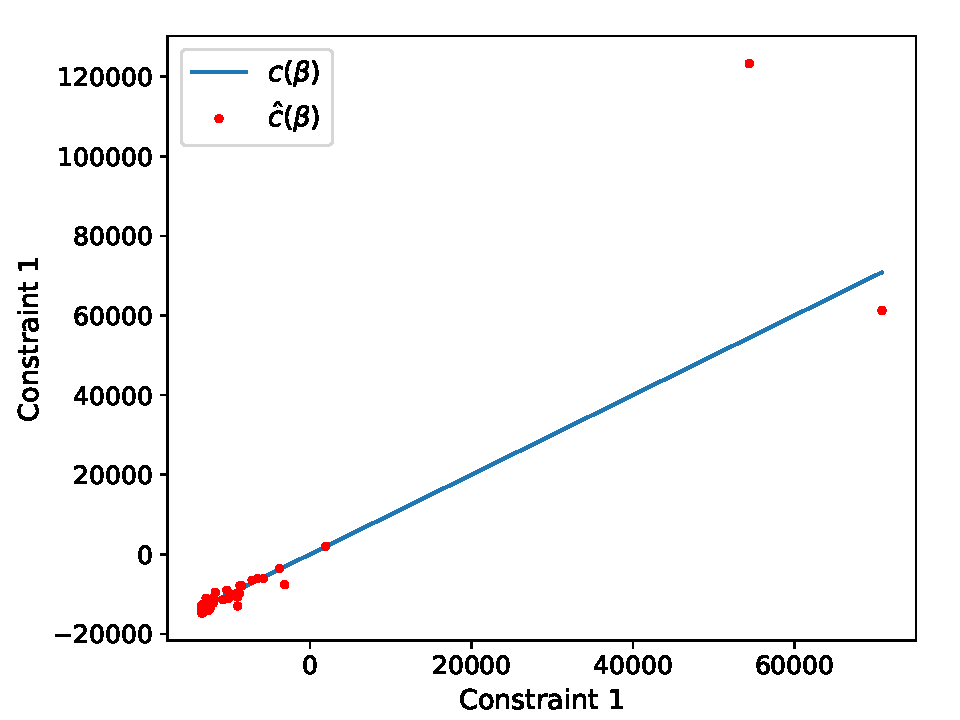
\includegraphics[width=\textwidth, height=0.58\textwidth, 
    scale=1]{welded_beam_con1_fitness_end.pdf}    
    \end{subfigure}
    \hfill
    \begin{subfigure}[b]{0.45\textwidth}
    \centering
    \caption{Initial $c_{2}$, $\mathrm{NRMSE} \!= \!0.00000249$}
    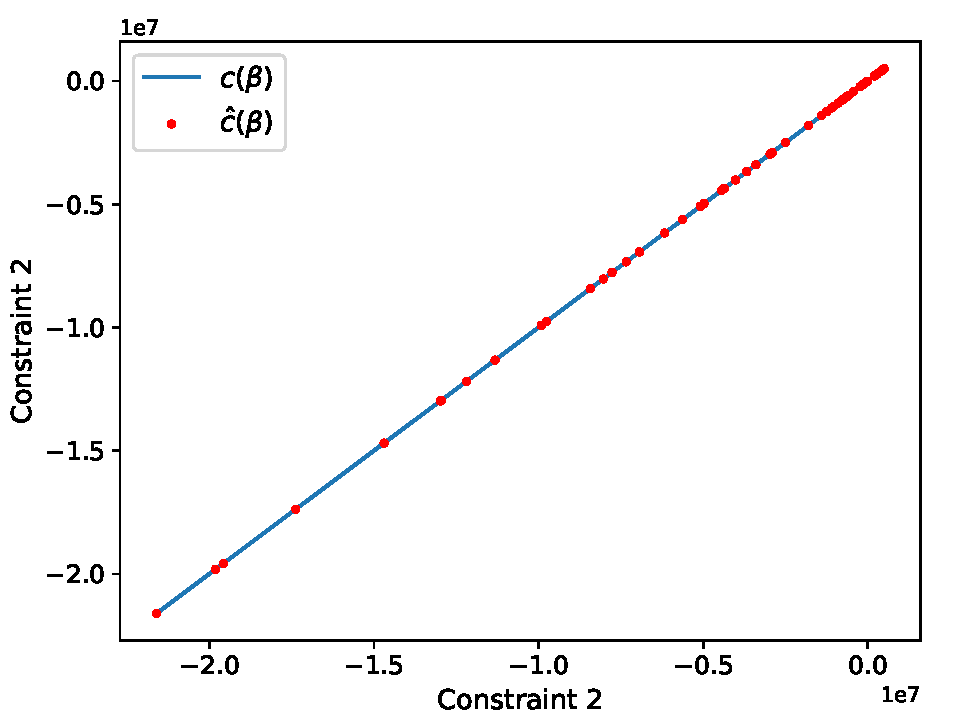
\includegraphics[width=\textwidth, height=0.58\textwidth, 
    scale=1]{welded_beam_con2_fitness_start.pdf}    
    \end{subfigure}
    \hfill
    \begin{subfigure}[b]{0.45\textwidth}
    \centering
    \caption{Final $c_{2}$, $\mathrm{NRMSE} \!= \!0.00000063$}
    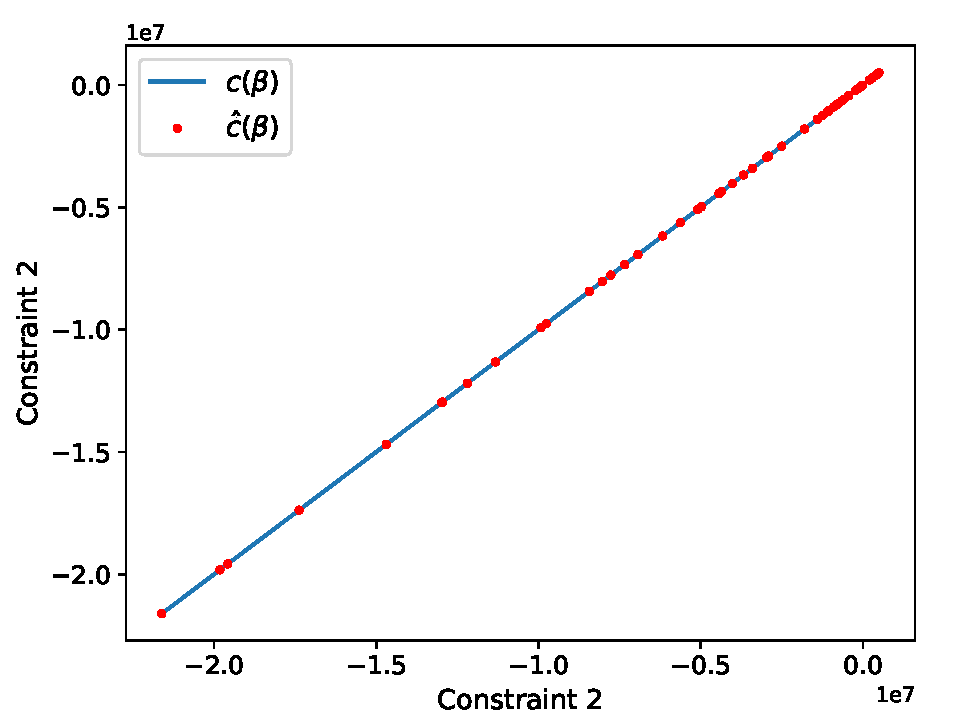
\includegraphics[width=\textwidth, height=0.58\textwidth, 
    scale=1]{welded_beam_con2_fitness_end.pdf}    
    \end{subfigure}
\caption{Case 3, welded beam case with RNG1. Deviation between 
exact $\mathrm{PSM}^{''}$ constraint values $\vec{c}(\vec{β})$ and 
Kriging predictions $\hat{\vec{c}}(\vec{β})$ given via the 
implementation of SMT. The initial Kriging model, which 
approximates the first two constraint functions, is trained on 
$n_{doe} \!= \!240$ and the final on $n_{doe}^{'} \!= \!429$ 
training patterns.}
\label{fig:fitting_con1_2_welded_beam}
\end{figure}

\newpage
%--------------------------------------------------------------

\begin{figure}[h!]
\centering
    \begin{subfigure}[b]{0.45\textwidth}
    \centering
    \caption{Initial $c_{3}$, $\mathrm{NRMSE} \!= \!0.00000008$}
    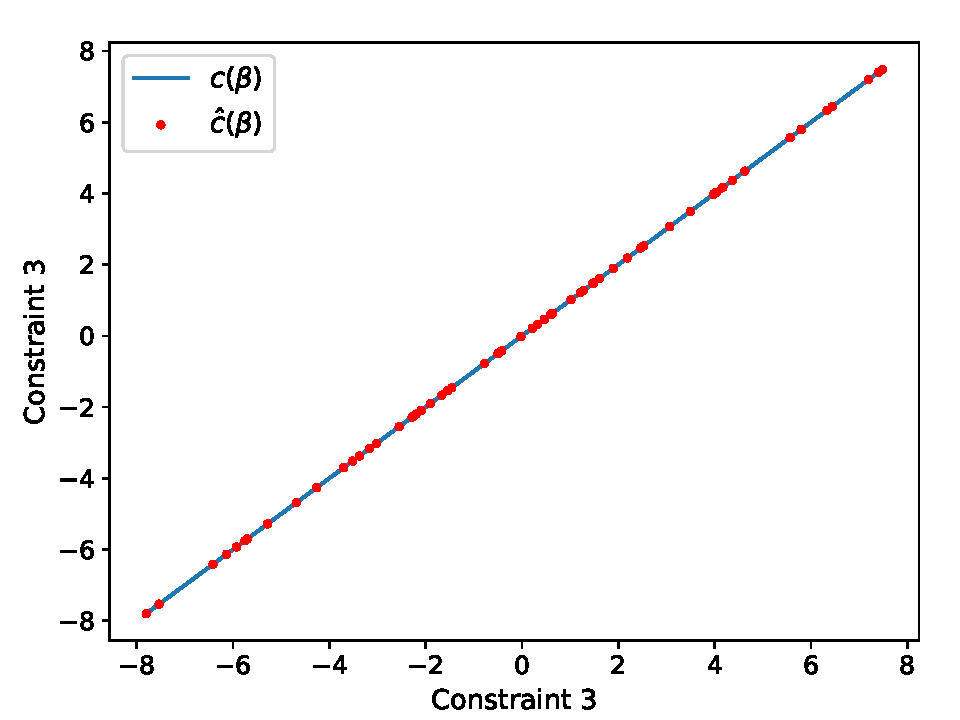
\includegraphics[width=\textwidth, height=0.6\textwidth, 
    scale=1]{welded_beam_con3_fitness_start.pdf}    
    \end{subfigure}
    \hfill
    \begin{subfigure}[b]{0.45\textwidth}
    \centering
    \caption{Final $c_{3}$, $\mathrm{NRMSE} \!= \!0.00000003$}
    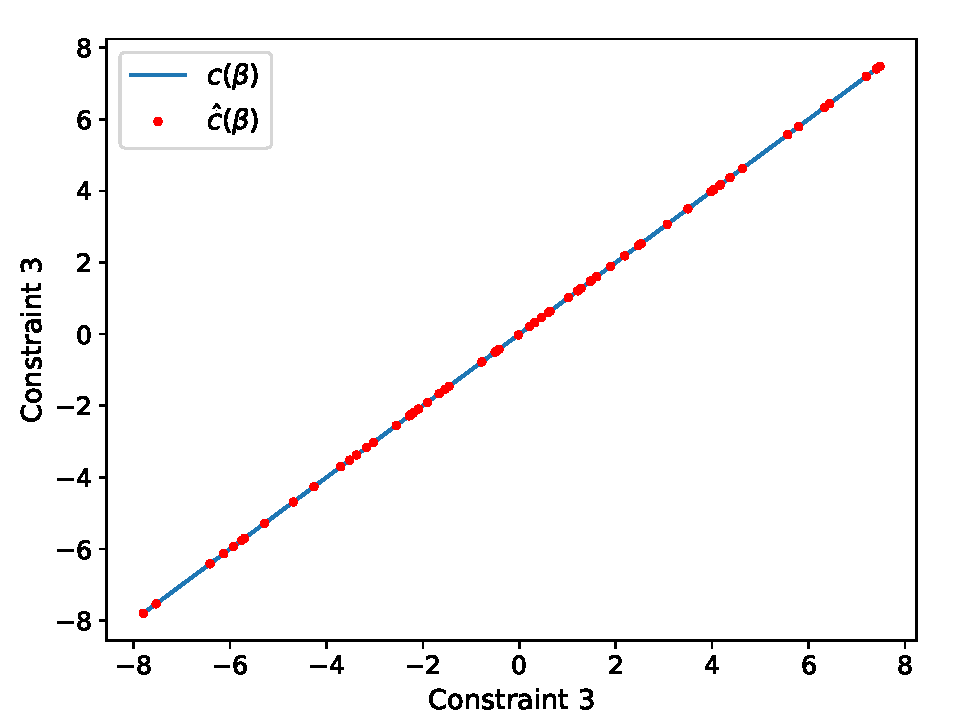
\includegraphics[width=\textwidth, height=0.6\textwidth, 
    scale=1]{welded_beam_con3_fitness_end.pdf}    
    \end{subfigure}
    \hfill
    \begin{subfigure}[b]{0.45\textwidth}
    \centering
    \caption{Initial $c_{4}$, $\mathrm{NRMSE} \!= \!0.00000617$}
    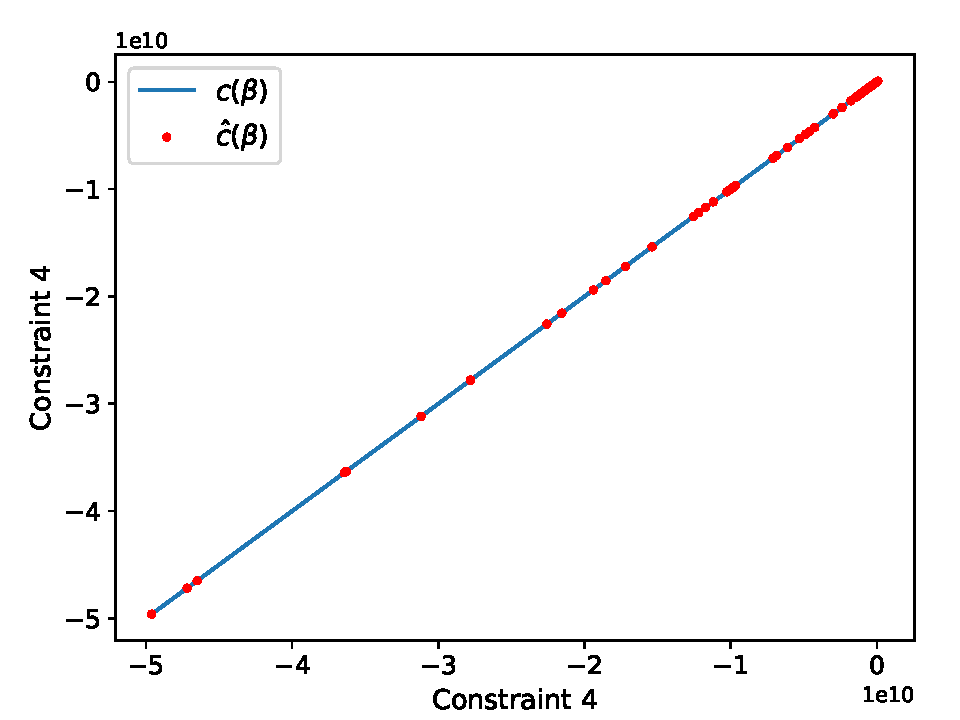
\includegraphics[width=\textwidth, height=0.6\textwidth, 
    scale=1]{welded_beam_con4_fitness_start.pdf}    
    \end{subfigure}
    \hfill
    \begin{subfigure}[b]{0.45\textwidth}
    \centering
    \caption{Initial $c_{4}$, $\mathrm{NRMSE} \!= \!0.00000131$}
    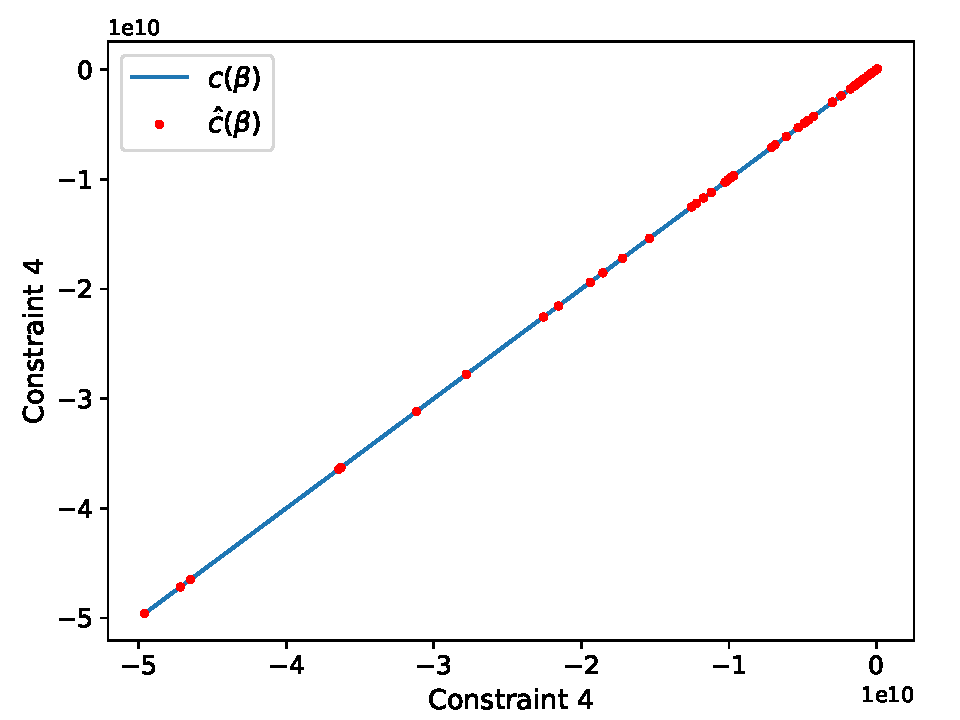
\includegraphics[width=\textwidth, height=0.6\textwidth, 
    scale=1]{welded_beam_con4_fitness_end.pdf}   
    \end{subfigure}
    \hfill
    \begin{subfigure}[b]{0.45\textwidth}
    \centering
    \caption{Final $c_{5}$, $\mathrm{NRMSE} \!= \!0.00000053$}
    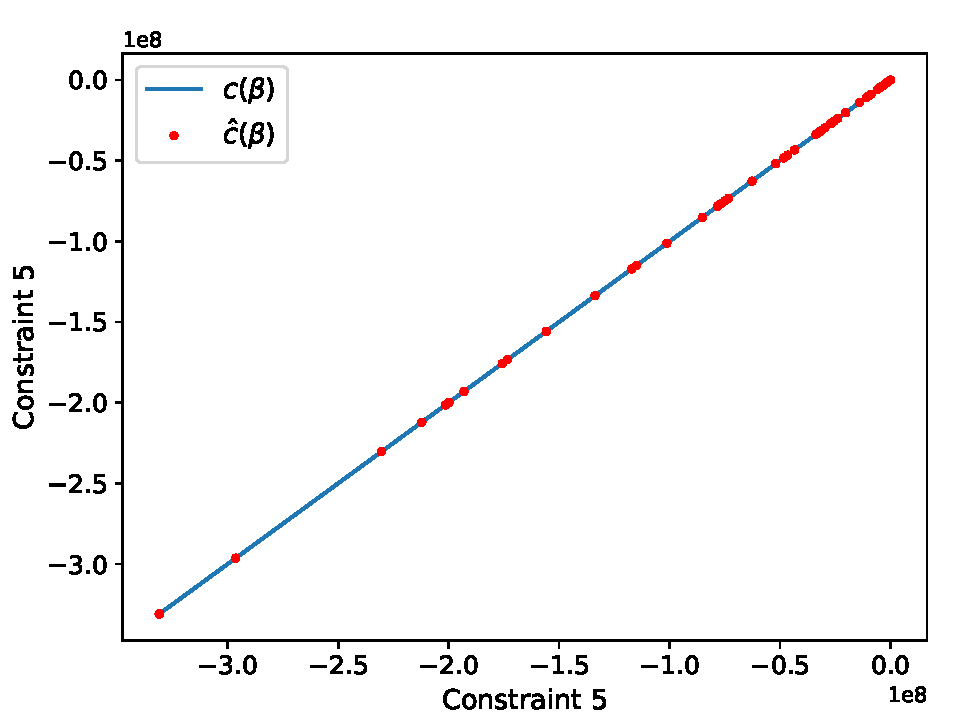
\includegraphics[width=\textwidth, height=0.6\textwidth, 
    scale=1]{welded_beam_con5_fitness_start.pdf}   
    \end{subfigure} 
    \hfill
    \begin{subfigure}[b]{0.45\textwidth}
    \centering
    \caption{Final $c_{5}$, $\mathrm{NRMSE} \!= \!0.00000014$}
    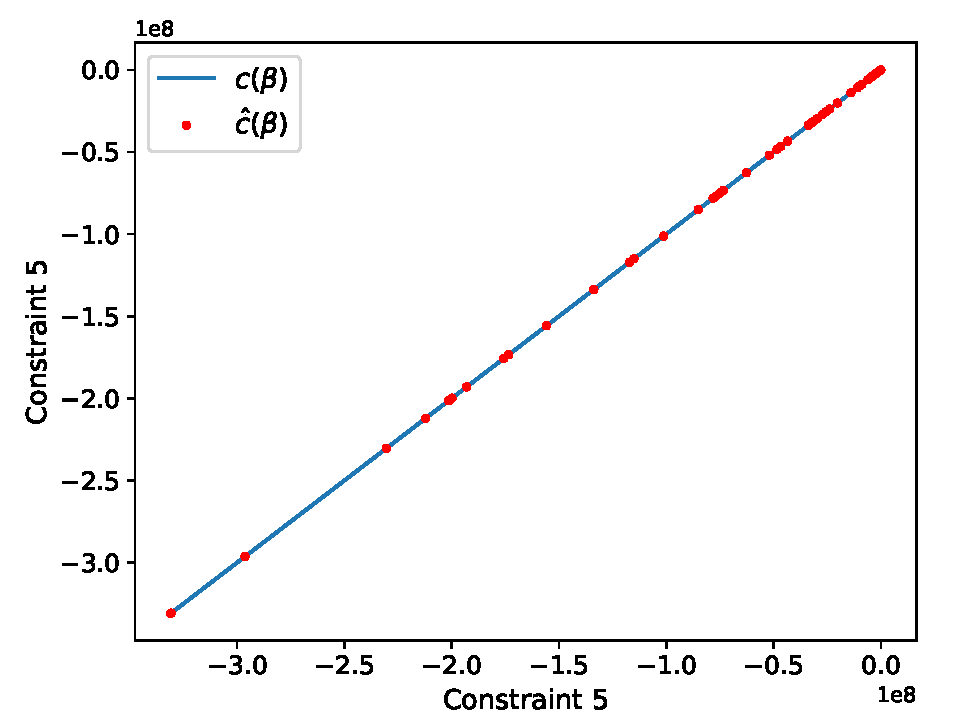
\includegraphics[width=\textwidth, height=0.6\textwidth, 
    scale=1]{welded_beam_con5_fitness_end.pdf}    
    \end{subfigure}
\caption{Case 3, welded beam case with RNG1. Deviation between 
exact PSM constraint values $\vec{c}(\vec{β})$ and RBF predictions 
$\hat{\vec{c}}(\vec{β})$ given via the implementation of SMT. The 
initial Kriging model, which approximates the remaining three 
constraint functions, is trained on $n_{doe} \!= \!240$ and the 
final on $n_{doe}^{'} \!= \!429$ training patterns.}
\label{fig:fitting_con3_5_welded_beam}
\end{figure}

The NRMSE calculates the mean normalised deviation between the 
predicted and exactly evaluated on the $\mathrm{PSM}^{''}$ values 
on $λ\!=\!60$ untried design sites $\mathbf{Β}$, where $\vec{β} 
\!= \!\vec{β}_{i} \!= \![β_{i,1}, β_{i,2}, \hdots, β_{i,n_{β}}] \in 
P_{λ}^{0}$ is any untried point in the design space contained in 
the initial offspring population set. NRMSE serves as a metric of 
model fitting and indicates that all trained metamodels are 
well-fitted, except from the one built on the 1st constraint 
function $c_{1}(\vec{β})$. This underfitted surrogate model hinders 
the convergence of the optimization process, which reaches an 
satisfactory optimal solution after 8 cycles. 

\newpage


%------------------------------------------------------------
%---------------On line----------------
%----------------------------------------------------------
\begin{itemize}
\item \textbf{Optimization using MAEAs with on-line trained 
matamodels}
\end{itemize}

In the MAEA-based optimization of welded beam design using on-line 
trained metamodels, the LCPE phase is set to initiate once 480 
exact evaluations are performed. In LCPE, personalised local
metamodels are trained on $20 \leq n_{t} \leq 21$ training 
patterns and subsequently  $2 \leq λ_{e} \leq 4$ individuals
are re-evaluated using the exact evaluation model. A total of 
10000 PSM evaluations are performed, unless 75
generations are formed without improving the current outcome, in 
which case the optimization terminates. Local metamodels are built 
by utilizing either the assisting software SMT or EASY. The former 
accommodates the use of Kriging, KPLS, KPLSK and RBFs, while the 
latter relies on Kriging and most often RBFs. In order to identify 
the most suitable metamodel in SMT for the welded beam 
optimization case, a comparison between each respective model 
is performed w.r.t. the convergence history and the produced 
outcome; the results of each comparison are presented in table 
figure \ref{fig:SMT_models_welded_beam} and table  
\ref{table:online_SMT_welded_beam}, respectively.  

\begin{figure}[h!]
\centering
	\begin{subfigure}[b]{0.49\textwidth}
	\centering
	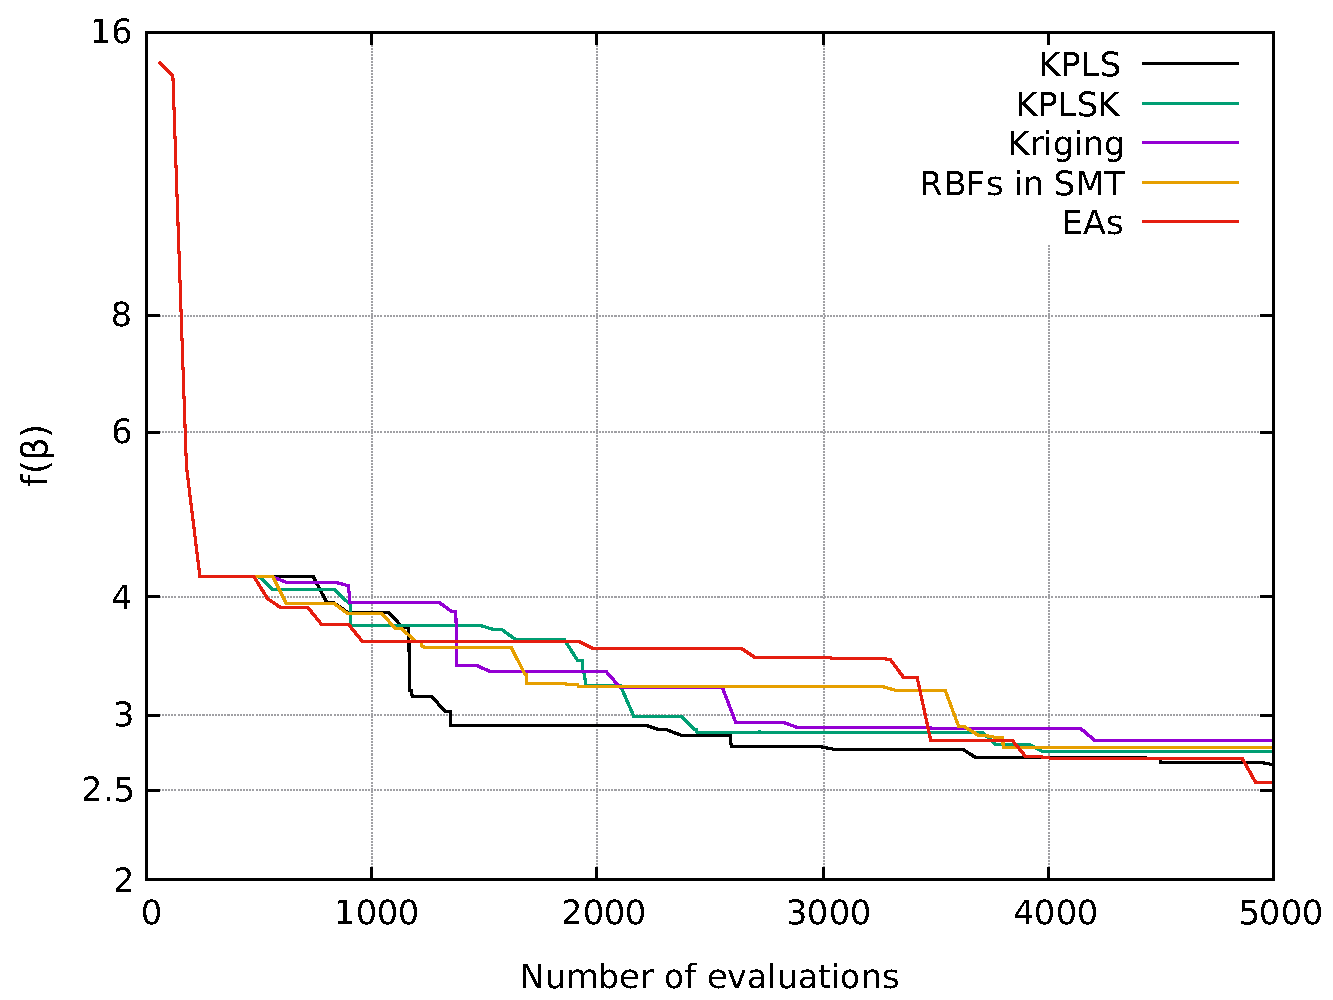
\includegraphics[width=\textwidth, height = 0.9\textwidth, 
	scale=1]{welded_beam_online_comparison.pdf}
	\end{subfigure}
	\hfill
	\begin{subfigure}[b]{0.49\textwidth}
	\centering
	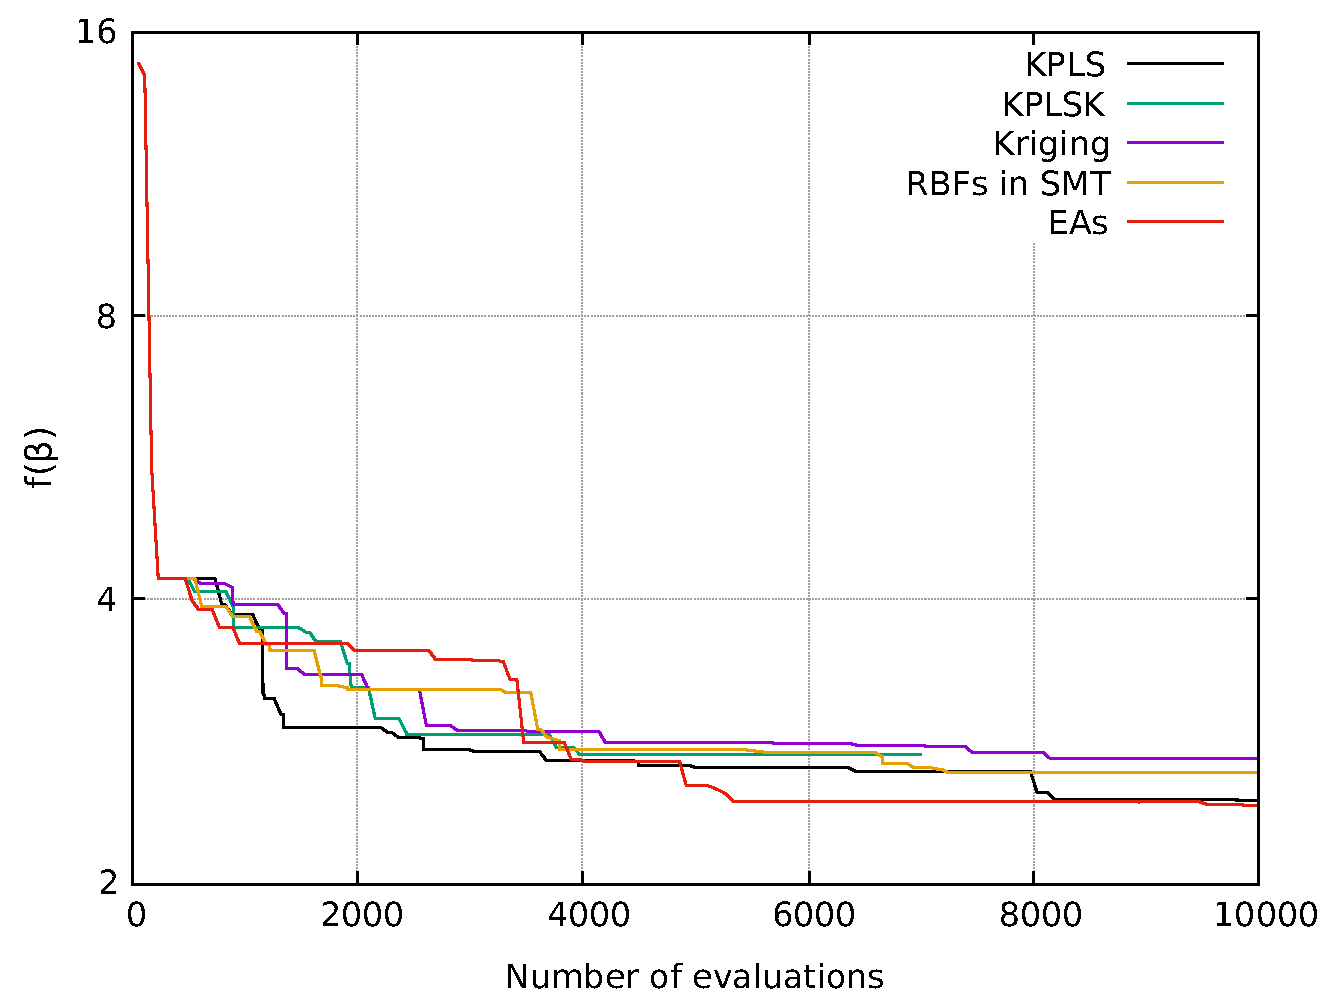
\includegraphics[width=\textwidth, height = 0.9\textwidth, 
	scale=1]{welded_beam_online_comparison2.pdf}
	\end{subfigure}   
\caption{Welded beam design with RNG1. Comparison between the 
convergence history of EAs and MAEAs with metamodels trained 
on-line via SMT} 
\label{fig:SMT_models_welded_beam}
\end{figure}

\begin{table}[h!]
\centering
%\rowcolors{2}{gray!30!}{white!50!gray!10}
\scalebox{0.83}{%
\begin{tabular}[c]{ |p{1.7cm}||p{1.6cm}|p{1.6cm}|p{1.6cm}|
p{1.6cm}|p{1.6cm}|}
\toprule
\multicolumn{6}{|c|}{\cellcolor{gray!30!} 
\textbf{Welded beam case}} \\
\midrule 
\textbf{MAEAs, on-line} & $(μ,λ)$ \textbf{population}  
& \textbf{KPLS} & \textbf{KPLSK} & \textbf{Kriging} 
& \textbf{RBFs} \\
\hline
\textbf{SMT} & (30, 100) & 2.45 & 2.74 & 2.72 & 2.62 \\
\bottomrule
\end{tabular}%
}
\caption{Welded beam case with RNG1. Optimal candidate solution 
found using metamodels trained on-line via SMT}
\label{table:online_SMT_welded_beam}
\end{table}

The comparison between convergence histories of the SMT built-in
metamodels, depicted in figure \ref{fig:SMT_models_welded_beam}, 
indicates that KPLS model is most suitable to facilitate the 
optimization of the welded beam case due to its fast convergence to 
the threshold of both 5000 and 10000 PSM evaluations. In plain EAs, 
RNG1 yields the best optimization outcome and for that reason MAEAs 
with on-line training are initialized with the same offspring 
population $P_{λ}^{0}$.

\newpage
%------------------------------------------------------------------


KPLS is yet to be compared to EASY built-in RBFs and plain EAs; 
the results are presented in table 
\ref{table:online_SMT_EASY_comparison_welded_beam}.
 
\begin{table}[h!]
\centering
%\rowcolors{2}{gray!30!}{white!50!gray!10}
\scalebox{0.87}{%
\begin{tabular}[c]{ |p{2.2cm}||p{1.5cm}|p{1.4cm}|p{1.4cm}|
p{1.8cm}|p{1.4cm}|p{2.4cm}|}
\toprule
\multicolumn{7}{|c|}{\cellcolor{gray!30!} 
\textbf{Welded beam design}} \\
\midrule 
\textbf{MAEAs, on-line} & $(μ,λ)$ \textbf{population} 
& \textbf{Best} & \textbf{Worst} & \textbf{Average} 
& \textbf{Avg. exact eval.} 
& \textbf{Avg. metamodel eval.}  \\
\hline
\textbf{SMT} & (20, 60) & 2.45 & 2.62 & 2.54 & 10000 & 11579 \\
\textbf{EASY} & (20, 60) & 2.38 & 2.82 & 2.53 & 10000 & 10738 \\
\hline
\textbf{Plain EAs} & (20, 60) & 2.42 & 3.05 & 2.59 & 10000 & - \\
\bottomrule
\end{tabular}%
}
\caption{Welded beam case. Comparison between the outcome of the  
optimization using MAEAs with on-line training and plain EAs}
\label{table:online_SMT_EASY_comparison_welded_beam}
\end{table}

The design variable vector that minimizes the construction
cost of the welded beam via the implementation of KLPS is $\vec{β} 
\!= \![0.234, 5.717, 9.276,$ $0.239]$. For MAEAs utilizing EASY 
built-in RBFs the respective optimal design variable vector is 
$\vec{β} = [0.255, 5.664, 8.527, 0.260]$.
 
\begin{figure}[h!]
\centering
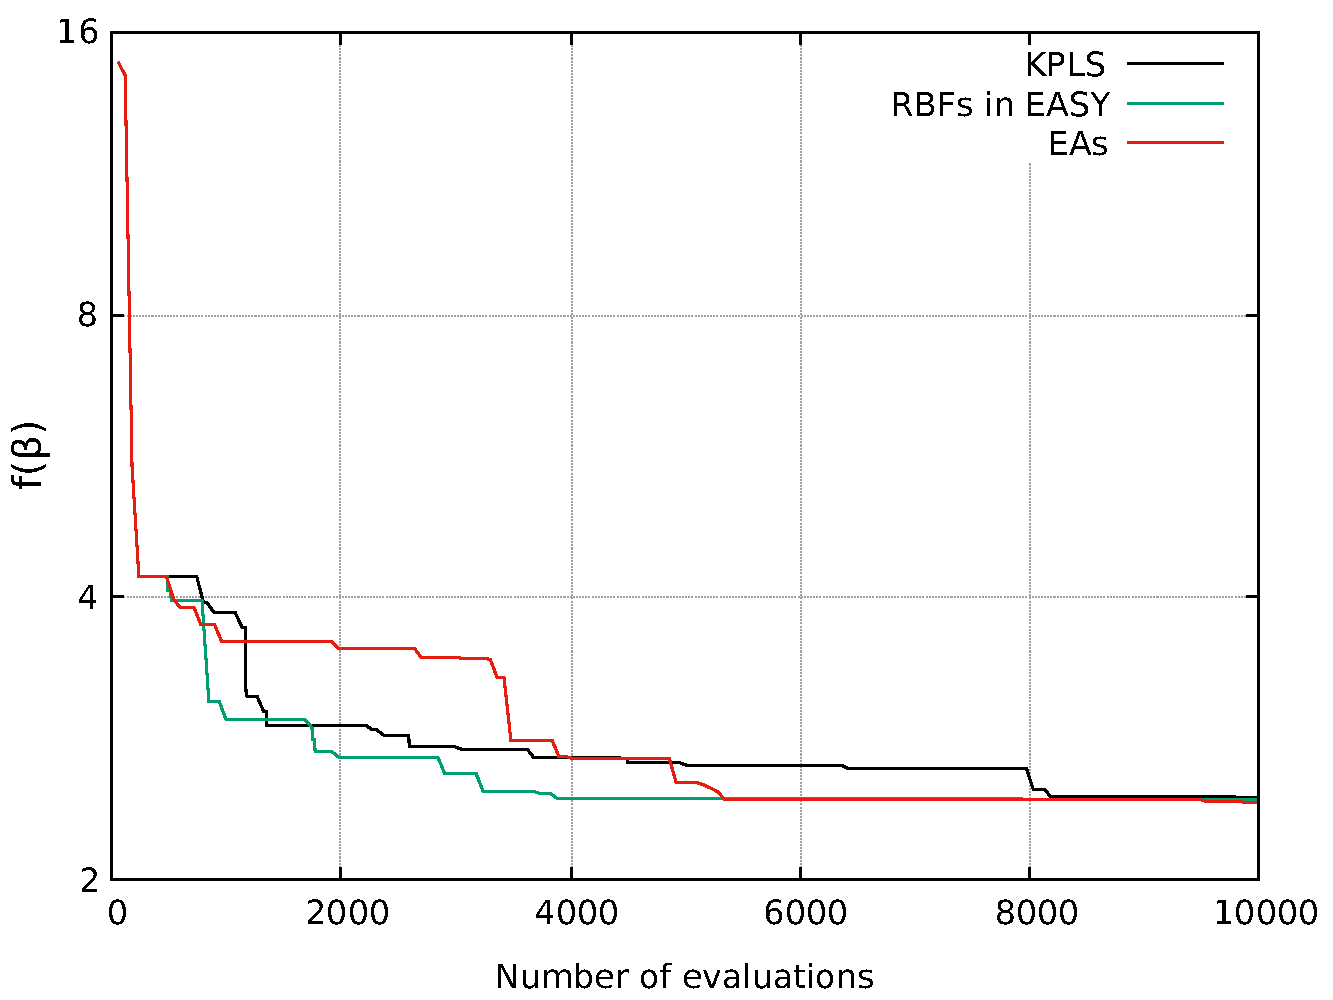
\includegraphics[width=0.68\textwidth, height=0.5\textwidth, 
scale=1]{welded_beam_online.pdf}   
\caption{Welded beam case with RNG1. Comparison between the 
convergence histories of the optimization using EAs and MAEAs 
with metamodels trained on-line via SMT and EASY} 
\label{fig:SMT_EASY_welded_beam}
\end{figure}

In the comparison of convergence histories depicted in figure 
\ref{fig:SMT_EASY_welded_beam}, EASY built-in RBFs are seemingly 
more accurate than KPLS model and yield a faster convergence. The 
impact of MAEAs on the computational cost is evident, since they 
outperform conventional EAs prior to the threshold of 10000 exact 
PSM evaluations.


\vfill

\newpage
%--------------------------------------------------------------


\subsection{MOO of Welded Beam Design}

The welded beam case appears in the majority of the scholar
literature as SOO problem, where the single objective is the 
minimization of the fabrication cost of the design. However, 
a variation of this optimization case also exists where the
welded beam design is optimized w.r.t. to two objectives, 
which are the fabrication cost of the design and the deflection 
$δ(\vec{β})$ of the beam. In this case, the deflection of the 
beam does not bound the design space of possible candidate 
solutions and the optimization problem assumes the following 
mathematical expression:
\begin{equation}
\begin{split}
min \hspace{2mm} & f_{1}(\vec{β}) = 1.10471β_{1}^{2}β_{2} + 
0.04811β_{3}β_{4}(14.0 + β_{2})
\\ &
f_{2}(\vec{β}) = \dfrac{2.1952}{β_{4}β_{3}^{3}} 
\\[0.3cm] 
\text{subject to} \hspace{2mm} & c_{1}(\vec{β}) = 
τ(\vec{β}) - τ_{max} \leq 0 
\\ &
c_{2}(\vec{β}) = σ(\vec{β}) - σ_{max} \leq 0
\\ &
c_{3}(\vec{β}) = β_{1} - β_{4} \leq 0
\\ &
c_{4}(\vec{β}) = P - P_{c}(\vec{β}) \leq 0
\end{split}
\end{equation}
\\[-2mm]
where the bounds of each design variable are $0.125 \leq 
β_{1} \leq 10.0$, $0.1 \leq β_{2} \leq 10.0$, $0.1 \leq β_{3} 
\leq 10.0$ and $0.1 \leq β_{4} \leq 10.0$. The formulas that 
describe $τ(\vec{β})$, $σ(\vec{β})$ and $P_{c}(\vec{β})$ can 
be found in equations \ref{welded_con1}, \ref{welded_con2} 
and \ref{welded_con5}, respectively. In this case, the 
objectives are conflicting and their corresponding values are 
presented in figure \ref{fig:Pareto_welded_beam}.

\begin{figure}[h!]
\centering
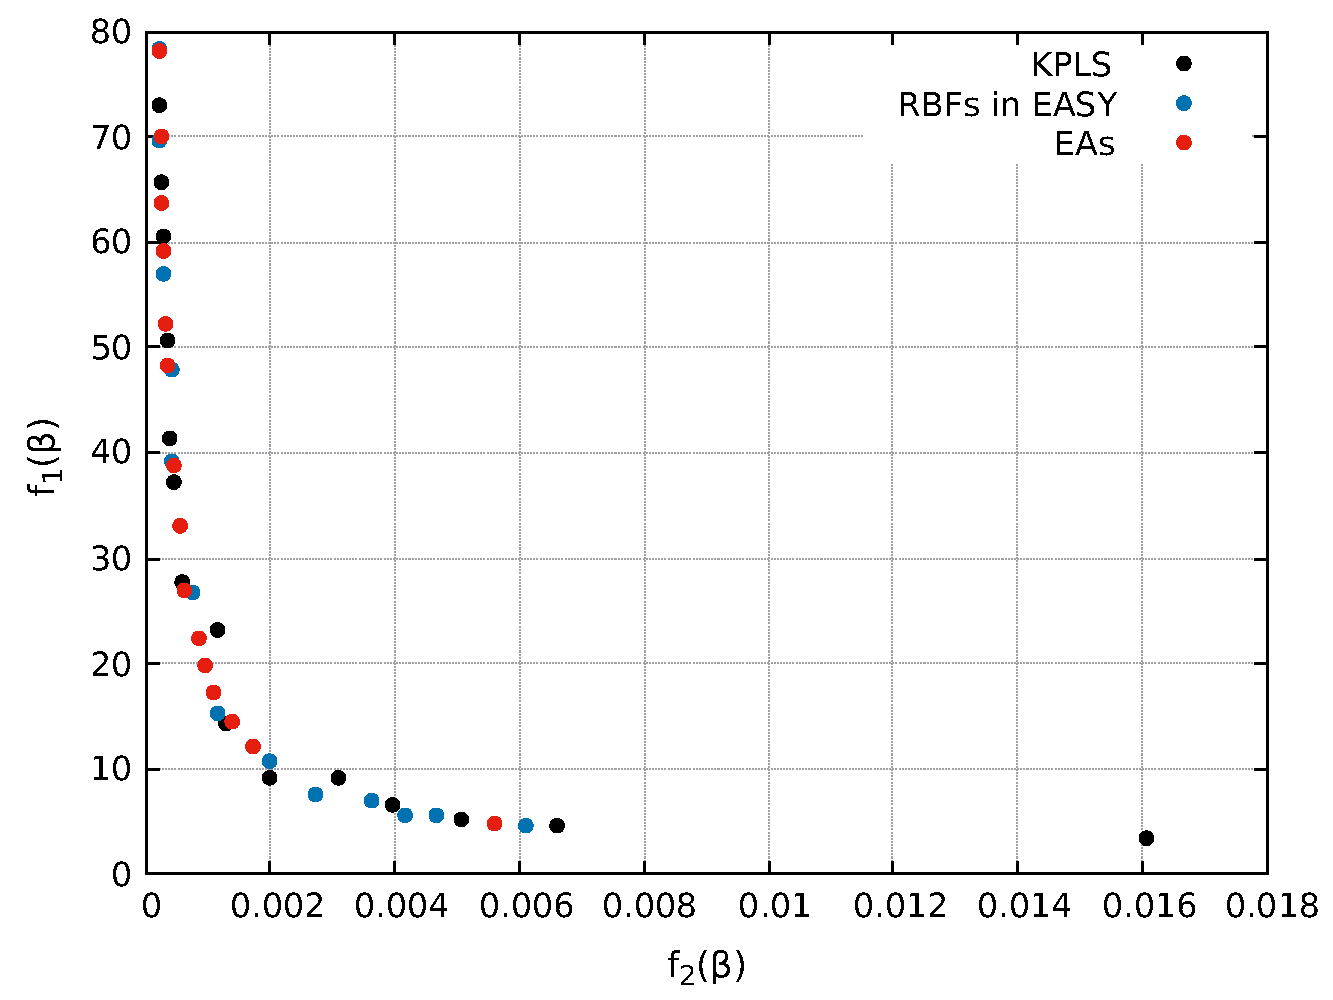
\includegraphics[width=0.57\textwidth]{pareto_welded_beam.pdf}
\caption{Pareto front of 15 non-dominated candidate solutions 
found in the MOO welded beam case for 1000 exact PSM evaluations} 
\label{fig:Pareto_welded_beam}
\end{figure}

The first two fronts are obtained by optimizing the MOO welded 
beam case via the use of MAEAs with on-line training, namely EASY 
built-in RBFs and the KPLS model found in SMT. The LCPE phase is 
set to initiate once 240 exact evaluations are performed on the 
PSM. In LCPE, personalised local metamodels are trained on $20 
\leq n_{t} \leq 21$ training patterns and subsequently  $2 \leq 
λ_{e} \leq 6$ individuals are re-evaluated using the exact 
evaluation model. The comparison is completed by the front that 
results from the optimization of the MOO case via the use of plain 
EAs. 

\newpage
%----------------------------------------------------------------


Since all fronts are seemingly overlapping, it is not evident 
which method yielded the best outcome. A way to determine this, 
is by calculating the hypervolume indicator \cite{hypervolume 
indicator} of each front $\mathcal{F} \subset \mathbb{R}^{n}$, 
which is defined as the measure of the region weakly dominated by 
$\mathcal{F}$ and bound by a reference point $\vec{x}_{r} \in 
\mathbb{R}^{n}$ and expressed as:

\begin{equation}
H(\mathcal{F}) = Λ \left( \{ \vec{p} \in \mathbb{R}^{n} | 
\hspace{1mm} \exists \vec{q} \in \mathcal{F}: \vec{q} \leq \vec{p} 
\hspace{2mm} \text{and} \hspace{2mm} \vec{p} \leq  \vec{x}_{r} \}
\right)
\end{equation} 
\\[-3mm]
where $H(\cdot)$ denotes the Lebesgue measure which is a way  
of assigning measure to subsets $\mathcal{F}$ of $n$-dimensional 
Euclidean space. In the 2D space, which is the case here, the 
Lebesgue measure $H(\mathcal{F})$ is equivalent to the area 
defined by each $\vec{q} \in \mathcal{F}$ and the reference point
$\vec{x}_{r} \in \mathbb{R}^{n}$. The coordinates ($x_{r_{1}}, 
x_{r_{2}}$) of the reference point in 2D space are defined as:
\begin{equation}
\begin{split}
& x_{r_{1}} \!= \! \{ q_{1} \in \mathcal{F}_{i}: q_{1} \geq ξ, 
\forall ξ \in \mathcal{F}_{i}, \forall i \in [1, n_{f}] \} + ξ_{1}
\\ &
x_{r_{2}}  \!= \! \{ q_{2} \in \mathcal{F}_{i}: q_{2} \geq ξ, 
\forall ξ \in \mathcal{F}_{i}, \forall i \in [1, n_{f}] \} + ξ_{2}
\end{split}
\end{equation}
\\[-2mm]
where $q_{1}, q_{2}$ are the coordinates of $\vec{q} \in 
\mathcal{F}$ point in 2D space, $n_{f}$ is the number of 
compared fronts and $ξ_{1}, ξ_{2}$ user-defined values. In this
case, the parameters assume the values $(ξ_{1}, ξ_{2}) = (0.002, 
20)$ and $(x_{r_{1}}, x_{r_{2}}) = (0.0181, 98.27)$ and 
yield the hypervolume indicators for each Pareto front shown in 
figure \ref{fig:hypervolume_welded_beam}.

\begin{figure}[h!]
\centering
	\begin{subfigure}[b]{0.45\textwidth}
	\centering
	\caption{KPLS, $H \!= \! 1.6222$ }
	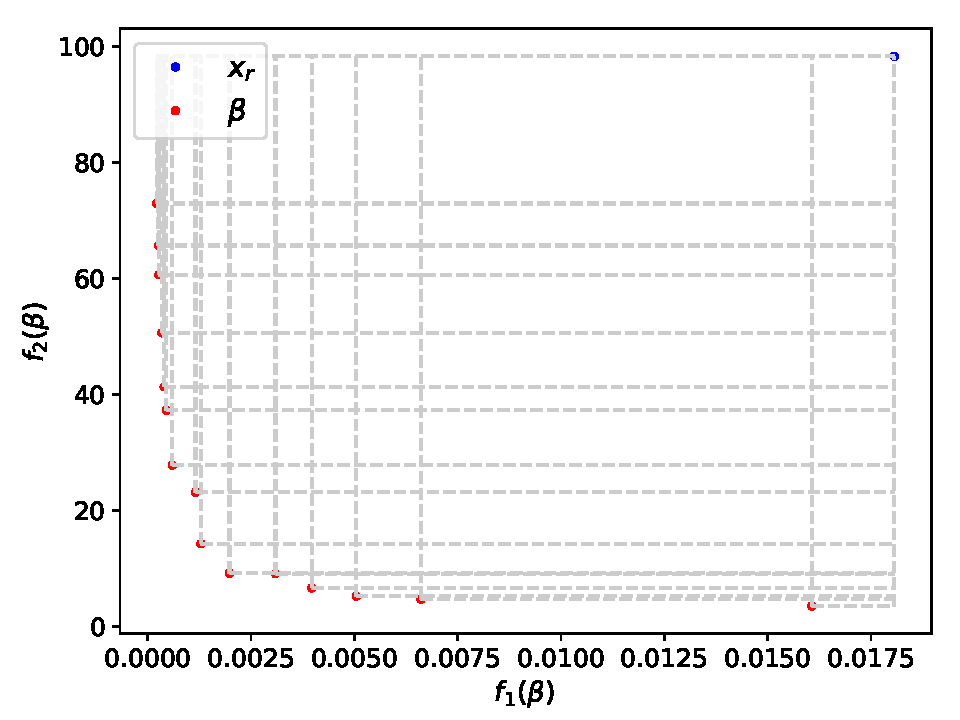
\includegraphics[width=\textwidth, height = 0.7\textwidth, 
	scale=1]{welded_beam_MOO_front1.pdf}
	\end{subfigure}
%--figure2
\hfill
	\begin{subfigure}[b]{0.45\textwidth}
	\centering
	\caption{RBFs in EASY, $H \!= \! 1.6215$ }
	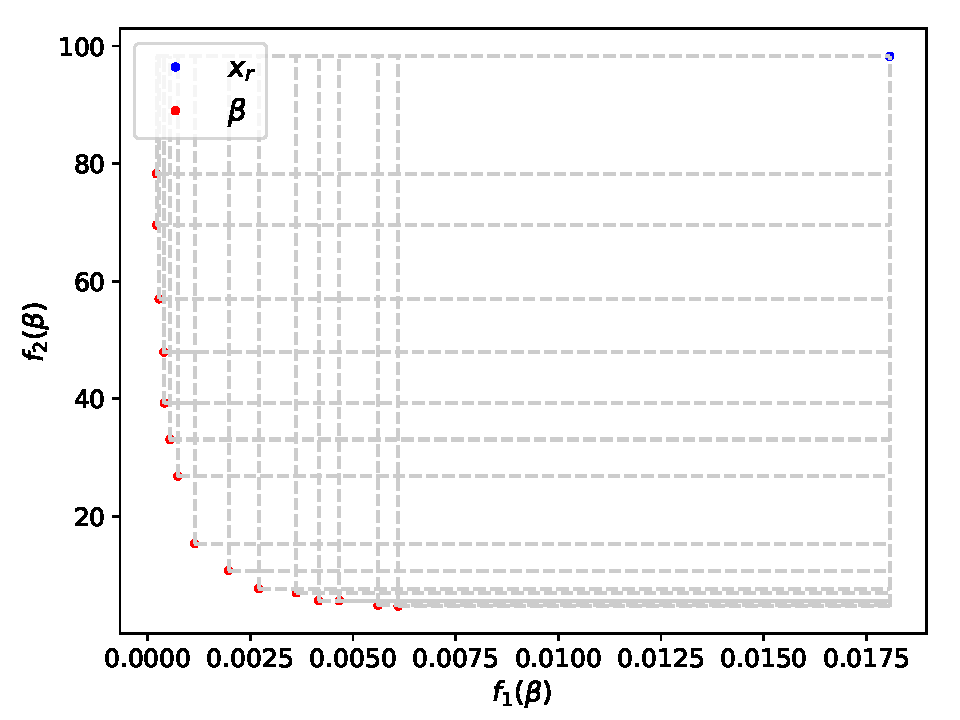
\includegraphics[width=\textwidth, height = 0.7\textwidth, 
	scale=1]{welded_beam_MOO_front2.pdf}
	\end{subfigure}
%-----figure3
\hfill
	\begin{subfigure}[b]{0.45\textwidth}
	\centering
	\caption{EAs, $H \!= \! 1.6061$ }
	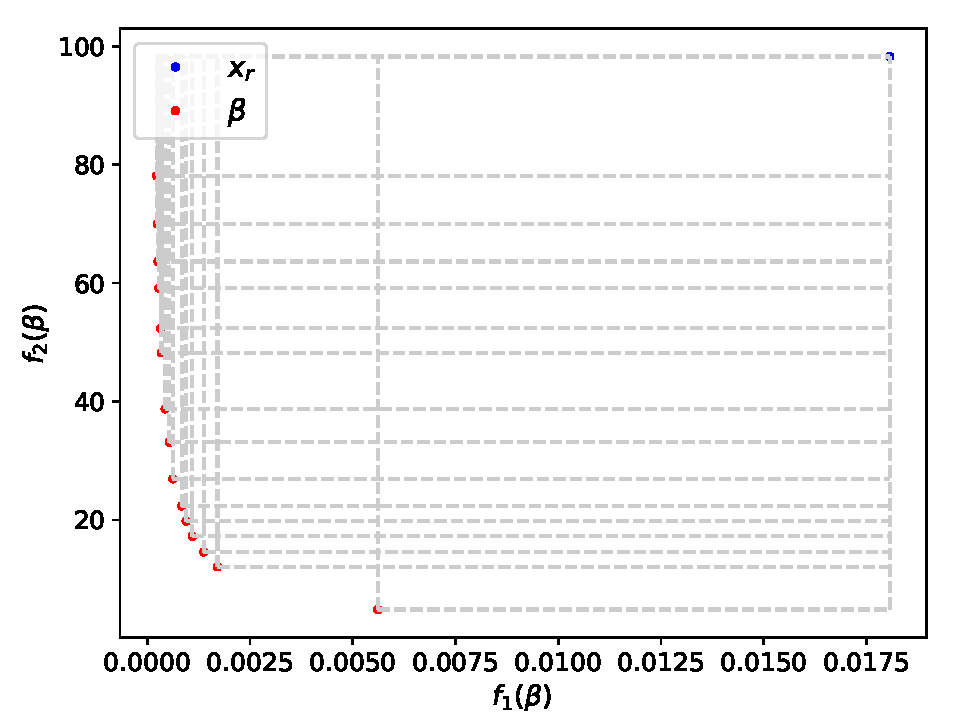
\includegraphics[width=\textwidth, height = 0.7\textwidth, 
	scale=1]{welded_beam_MOO_front3.pdf}
	\end{subfigure}
\caption{MOO welded beam case. Hypervolume indicator $H$ for 
fronts formed via the use of EAs, on-line trained KPLS and 
RBFs in EASY}
\label{fig:hypervolume_welded_beam}
\end{figure}

According to the $H$ value, the best front is the one formed via 
the use of on-line trained KPLS. Consequently, $\vec{β} = 
[0.481, 3.383, 6.572, 0.481]$ is selected that yields the response 
$(f_{1}, f_{2}) \!= \!(6.41, \hspace{1mm} 0.0031)$, since a 
minor increase in beam deflection yields a significant decrease in 
the fabrication cost.

\newpage
%---------------------------------------------------


\section{Speed Reducer Design}

The second optimization case is the SOO problem of minimizing
the overall weight of a speed reducer. This design is used to 
reduce the output speed by increasing the output torque via
the use two gears that are mounted to two separate shafts of
diameter $d_{1}$ and $d_{2}$. The structure is enclosed 
within a housing, while a pair of pairings is used at the 
connection point of each shaft in order to reduce friction 
produced by the rotation movement of the shafts (see figure 
\ref{fig:speed_reducer_image}). The minimization of the overall 
weight of the structure is, therefore, refers to the minimization 
of the total weight of both gears and shafts. The speed reducer 
case\cite{Golinski} is optimized w.r.t. the following design 
variables:

\begin{itemize}
\item Face width of the gear $b$ in [cm], 
where $2.6 \leq β_{1} \leq 3.6$ 
\item Teeth module $m$ in [cm], where $0.7\leq β_{2}\leq 0.8$
\item Number of pining teeth $N_{teeth}$,
where $17 \leq β_{3} \leq 28$
\item Length between bearings of the first shaft $L_{1}$ in 
[cm], where $7.3 \leq β_{4} \leq 8.3$ 
\item Length between bearings of the second shaft $L_{2}$ in 
[cm], where $7.3 \leq β_{5} \leq 8.3$ 
\item Diameter of the first shaft $d_{1}$ in [cm],
where $2.9 \leq β_{6} \leq 3.9$ 
\item Diameter of the second shaft $d_{2}$ in [cm],
where $5.0 \leq β_{7} \leq 5.5$ 
\end{itemize}

\begin{figure}[h!]
\centering
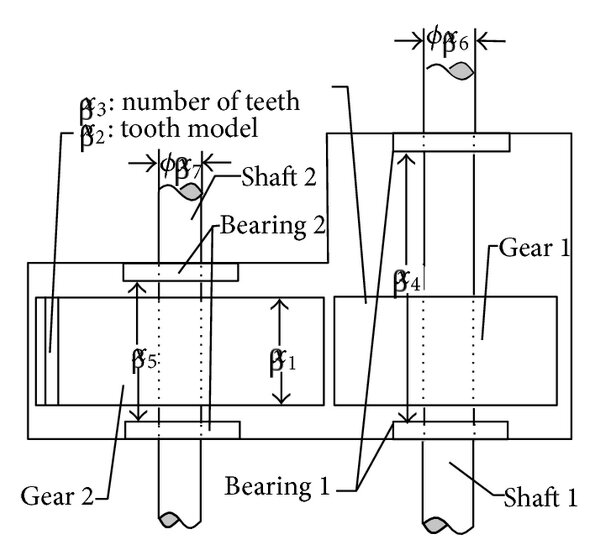
\includegraphics[width=0.6\textwidth]{speed_reducer}   
\caption{Speed reducer design} 
\label{fig:speed_reducer_image}
\end{figure}

\newpage
%----------------------------------------------------------


The volume of the speed reducer in [$cm^{3}$] can be 
calculated using the following equation \cite{speed reducer}, 
which multiplied by the density of the material yields the 
weight of the speed reducer:
\begin{equation}
\begin{split}
W_{spr} = \hspace{2mm} &  c_{1}bm^{2} \left( c_{2} 
N_{teeth}^{2} + c_{3} N_{teeth} - c_{4} \right) - c_{5}
\left( d_{1}^{\hspace{1mm}2} + d_{2}^{\hspace{1mm}2} \right) 
\\ &
c_{6} \left( d_{1}^{\hspace{1mm}3} + d_{2}^{\hspace{1mm}3} 
\right) + c_{1} \left( L_{1}d_{1}^{\hspace{1mm}2} 
+ L_{2}d_{2}^{\hspace{1mm}2} \right)
\end{split} 
\end{equation}

where the occurring parameters are calculated by Golinski 
\cite{Golinski}:
\begin{itemize}
\item $c_{1} = 0.7854$
\item $c_{2} = 3.3333$
\item $c_{3} = 14.9334$
\item $c_{4} = 43.0934$
\item $c_{5} = 1.508$
\item $c_{6} = 7.4777$
\end{itemize} 
\vspace{3mm}
and thus the previous equation can be restated as such:
\begin{equation}
\begin{split}
W_{spr} = \hspace{2mm} &  0.7854bm^{2} \left( 3.3333 
N_{teeth}^{2} + 14.9334 N_{teeth} - 43.0934 \right) - 1.508
\left( d_{1}^{\hspace{1mm}2} + d_{2}^{\hspace{1mm}2} \right) 
\\ &
7.4777 \left( d_{1}^{\hspace{1mm}3} + d_{2}^{\hspace{1mm}3} 
\right) + 0.7854 \left( L_{1}d_{1}^{\hspace{1mm}2} 
+ L_{2}d_{2}^{\hspace{1mm}2} \right)
\end{split} 
\end{equation}

The volume function is optimized in $\mathbb{R}^{7}$ space	
formed by the design variables $\{ b, m, N_{teeth}, L_{1}, 
L_{2}, d_{1}, d_{2} \}$. The design space is bound by the 
imposed constraints that are associated with limitations on 
the bending stress of gear teeth, surface stresses, transverse 
deflections of the shafts due to transmitted force and 
stresses in shafts. Subsequently the imposed constraints are
presented analytically. The upper bound on the bending stress 
of a gear tooth is given by the following formula:
\begin{equation}
σ_{g} = \dfrac{2M_{g}}{Ybm^{2}N_{teeth}} \leq σ_{g_{max}} 
\Rightarrow 
\dfrac{27}{bm^{2} N_{teeth}} \leq 1
\end{equation}
\\
where $Y = 0.3937$ is the Lewis tooth form factor, $M_{g}$
the bending moment for the gear teeth and $σ_{g_{max}} = 900 
\hspace{2mm} g/cm^{2}$ is the maximum bending stress of the 
gear teeth. Similarly the upper bound of the compressive stress of 
a gear tooth for both gears is defined as such:
\begin{equation}
P_{g_{1,2}} = \dfrac{2BM_{g}}{bm^{2}N_{teeth}^{2}} \leq  
P_{g_{max1,2}} \Rightarrow
\dfrac{397.5}{bm^{2}N_{teeth}^{2}} \leq 1
\end{equation}
\\
where $P_{g_{max1,2}} = 5800 \hspace{2mm} g/cm^{2}$ is the 
maximum surface compressive stress for both gears and $B$ is 
a coefficient dependent on Young's modulus of elasticity $E$.
\newpage
%----------------------------------------------------------


The transverse deflections of the shafts due to the 
transmitted load $P$ are required to not exceed the following
bounds:
\begin{equation}
\text{Shaft 1:} \hspace{5mm} 
δ_{1} = \dfrac{1}{48} \dfrac{PL_{1}^{2}}{EI_{1}} \leq δ_{1max}
\Rightarrow
\dfrac{1.93L_{1}^{3}}{mN_{teeth}
d_{1}^{\hspace{1mm}4}} \leq 1
\end{equation}

\begin{equation}
\text{Shaft 2:} \hspace{5mm}
δ_{2} = \dfrac{1}{48} \dfrac{PL_{2}^{2}}{EI_{2}} \leq δ_{2max}
\Rightarrow
\dfrac{1.93L_{2}^{3}}{mN_{teeth}
d_{2}^{\hspace{1mm}4}} \leq 1
\end{equation}
\\
where $I$ is the moment of inertia of the shafts and 
$δ_{1max}, δ_{2max}$ the maximum permissible transverse 
deflections of shaft 1 and 2 respectively.
\\
Subsequently, the bending stress conditions for the shafts are 
limited based on the following formulas:
\begin{equation}
\text{Shaft 1:} \hspace{5mm}
σ_{g_{1}} =  \dfrac{M_{z_{1}}}{W_{x_{1}}} \leq σ_{g_{1max}}
\Rightarrow
\dfrac{\sqrt{ \left( \dfrac{745L_{1}}{mN_{teeth}} \right)^{2} 
+ 16.9 \times 10^{6} }}{0.1d_{1}^{\hspace{1mm}3}} \leq 1100
\end{equation}

\begin{equation}
\text{Shaft 2:} \hspace{5mm} 
σ_{g_{2}} =  \dfrac{M_{z_{2}}}{W_{x_{2}}} \leq σ_{g_{2max}}
\Rightarrow
\dfrac{\sqrt{ \left( \dfrac{745L_{2}}{mN_{teeth}} \right)^{2} 
+  157.5 \times 10^{6} }}{0.1d_{2}^{\hspace{1mm}3}} \leq 850
\end{equation}
\\
where $σ_{g_{1max}} = 1100 \hspace{2mm} g/cm^{2}$, 
$σ_{g_{2max}} = 850 \hspace{2mm} g/cm^{2}$ are the maximum
permissible bending stresses for shaft 1 and 2, respectively.
$W_{x}$ is strength section modulus if each shaft and $M_{z}$
is moment of each shaft formulated by the equation:

$$ M_{z} = \sqrt{M_{g}^{2} + 0.75M_{s}^{2}} $$
\\[-0.2cm]
where $M_{s}$ is the torsional moment of each shaft.
\\
In order to improve the optimization process, various 
dimensional restrictions are applied based on experience:

\begin{equation}
i) \hspace{2mm}	\dfrac{mN_{teeth}}{40} \leq 1 \hspace{10mm} 
ii) \hspace{2mm} \dfrac{5m}{b} \leq 1 \hspace{10mm}
iii) \hspace{2mm} \dfrac{b}{12m} \leq 1
\end{equation}
\\
Similarly a pair of restrictions are applied on the dimensions 
of shafts based on previous experience:
\begin{equation}
\begin{split}
& 1.5d_{1} + 1.9 \leq L_{1}
\\ &
1.1d_{2} + 1.9 \leq L_{2}
\end{split}
\end{equation}  

\newpage
%-------------------------------------------------------


The final optimization case is formulated as such:
\begin{equation}
\begin{split}
min \hspace{2mm} f(\vec{β}) = \hspace{2mm} & 
0.7854bm^{2} \left( 3.3333 N_{teeth}^{2} + 14.9334 N_{teeth} 
- 43.0934 \right) - 1.508\left( d_{1}^{\hspace{1mm}2} + 
d_{2}^{\hspace{1mm}2} \right) 
\\ &
7.4777 \left( d_{1}^{\hspace{1mm}3} + d_{2}^{\hspace{1mm}3} 
\right) + 0.7854 \left( L_{1}d_{1}^{\hspace{1mm}2} 
+ L_{2}d_{2}^{\hspace{1mm}2} \right)
\\[0.4cm]
\text{subject to} \hspace{2mm} & c_{1}(\vec{β}) = 
\dfrac{27}{β_{1}β_{2}^{\hspace{1mm}2} β_{3}} -1 \leq 0
\\[0.3cm] &
c_{2}(\vec{β}) = \dfrac{397.5}{β_{1}β_{2}^{\hspace{1mm}2} 
β_{3}^{\hspace{1mm}2}} - 1 
\leq 0
\\[0.3cm] &
c_{3}(\vec{β}) = \dfrac{1.93β_{4}^{\hspace{1mm}3}}{β_{2}β_{3}
β_{6}^{\hspace{1mm}4}} - 1 \leq 0
\\[0.3cm] &
c_{4}(\vec{β}) = \dfrac{1.93β_{5}^{\hspace{1mm}3}}{β_{2}β_{3}
d_{7}^{\hspace{1mm}4}} - 1 \leq 0
\\[0.3cm] &
c_{5}(\vec{β}) = \dfrac{\sqrt{ \left( \dfrac{ 745β_{4} }{β_{2}
β_{3}} \right)^{2} + 
16.9 \times 10^{6} }}{110β_{6}^{\hspace{1mm}3}} - 1 \leq 0
\\[0.3cm] &
c_{6}(\vec{β}) = \dfrac{\sqrt{ \left( \dfrac{ 745β_{5} }{β_{2}
β_{3}} \right)^{2} 
+ 16.9 \times 10^{6} }}{85β_{7}^{\hspace{1mm}3}} - 1 \leq 0
\\[0.3cm] &
c_{7}(\vec{β}) = \dfrac{β_{2}β_{3}}{40} - 1 \leq 0
\\[0.3cm] &
c_{8}(\vec{β}) = \dfrac{5β_{2}}{β_{1}} - 1 \leq 0
\\[0.3cm] &
c_{9}(\vec{β}) = \dfrac{β_{1}}{12β_{2}} - 1 \leq 0
\\[0.3cm] &
c_{10}(\vec{β}) = \dfrac{1.5β_{6} + 1.9}{β_{4}} - 1 \leq 0
 \\[0.3cm] &
c_{11}(\vec{β}) = \dfrac{1.5β_{7} + 1.9}{β_{5}} - 1 \leq 0
\end{split}
\end{equation}

where the bounds of each design variable are $2.6 \leq β_{1} \leq 
3.6$, $\hspace{1mm} 0.7\leq β_{2}\leq 0.8$, $17 \leq β_{3} \leq 
28$, $\hspace{1mm} 7.3 \leq β_{4} \leq 8.3$, $\hspace{1mm} 7.3 
\leq β_{5} \leq 8.3$, $\hspace{1mm} 2.9 \leq β_{6} \leq 
3.9$, and $5.0 \leq β_{7} \leq 5.5$

\newpage
%-------EAs----------
%------------------------------------------------------
\begin{itemize}
\item \textbf{Optimization using EAs}
\end{itemize}

The optimization of the speed reducer design is performed via the 
use of plain EAs that utilize the PSM. Multiple experiments 
concluded that the optimal number of offspring and parent 
population is $(μ,λ) = (30, 100)$ where 5 parents are combined to 
create a single offspring with two-point crossover. Gray binary 
encoding is used where 12 bits are assigned to each design 
variable, except for $β_{2}, β_{3}$ and $β_{7}$ that are assigned 
8, 8 and 11 bits respectively. The optimization process terminates 
after 52000 total PSM evaluations have been performed 
and is repeated for 5 randomly initialised offspring populations 
$P_{λ}^{0}$ via the use of a RNG. The results are presented in
in table \ref{table:EAs_speed_reducer} and figure 
\ref{fig:EAs_speed_reducer}.
\begin{table}[h!]
\centering
%\rowcolors{2}{gray!30!}{white!50!gray!10}
\scalebox{0.84}{%
\begin{tabular}[c]{ |p{1.3cm}||p{1.6cm}|p{1.4cm}|p{1.4cm}|
p{1.8cm}|p{1.6cm}|p{1.6cm}| }
\toprule
\multicolumn{7}{|c|}{\cellcolor{gray!30!} 
\textbf{Speed reducer design}} \\
\midrule 
& $(μ,λ)$ \textbf{population} & \textbf{Best} & 
\textbf{Worst} & \textbf{Average} & \textbf{Exact model eval.} 
& \textbf{Average exact eval.} \\
\hline
\textbf{EAs} & (30, 100) & 2994.91 & 3001.97 & 2997.74 
& 52207 & 40246 \\
\bottomrule
\end{tabular}%
}
\caption{Optimization of speed reducer design using EAs}
\label{table:EAs_speed_reducer}
\end{table}

\vspace{-3mm}

\begin{figure}[h!]
\centering
	\begin{subfigure}[b]{0.47\textwidth}
    \centering
    \caption{Comparison between the convergence histories of 5 
    different $P_{λ}^{0}$ initializations}
    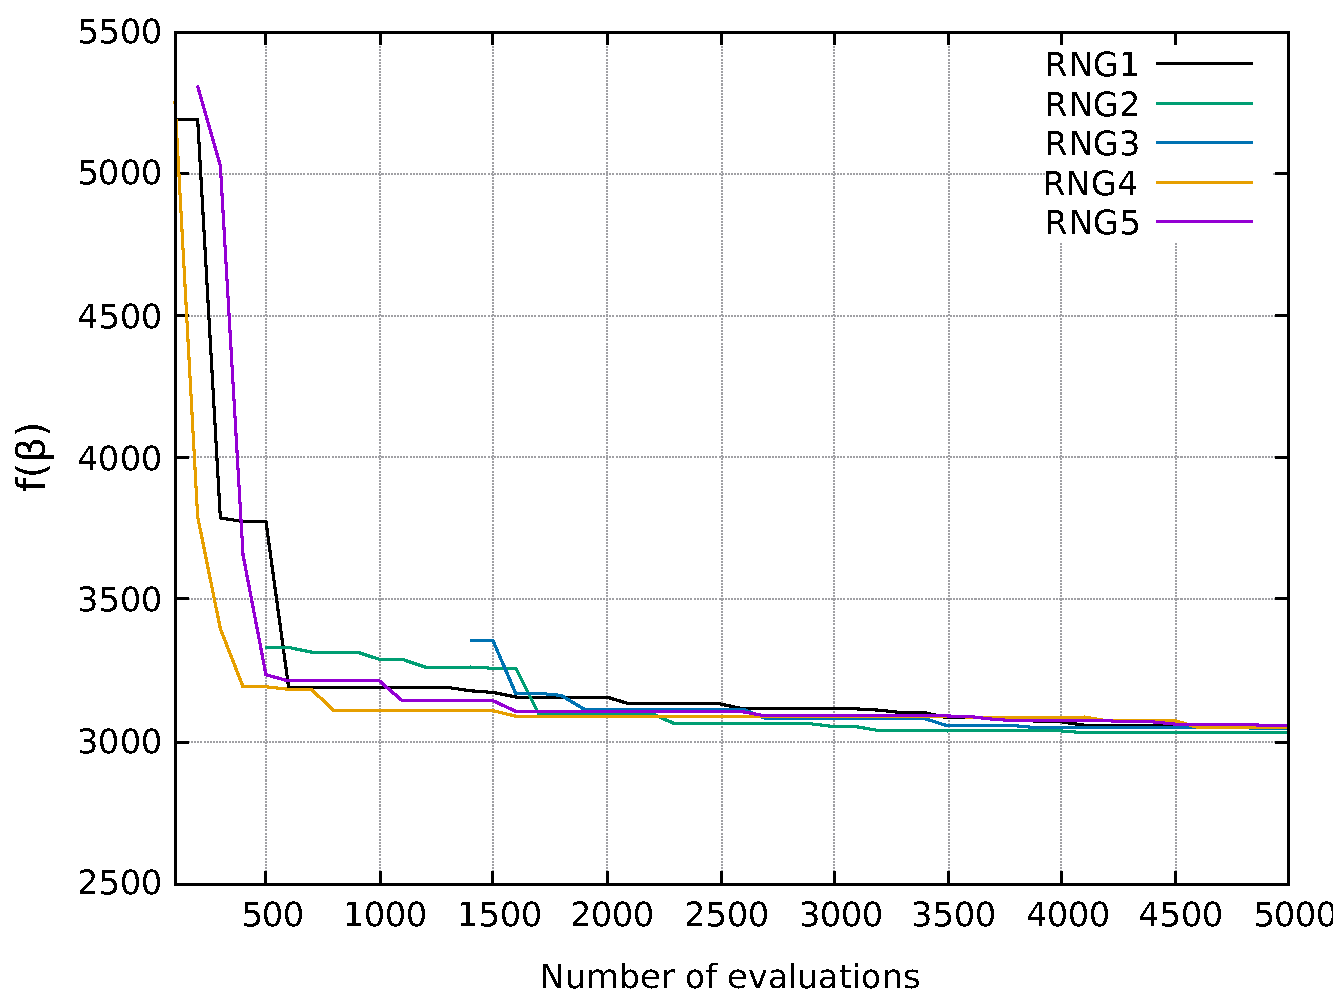
\includegraphics[width=\textwidth]{speed_reducer_ea1.pdf}    
    \end{subfigure}
    \hfill
    \begin{subfigure}[b]{0.47\textwidth}
    \centering
    \caption{Comparison between the convergence histories if 
    $f(\vec{β})$ range is narrowed}
    \includegraphics[width=\textwidth]{speed_reducer_ea2.pdf}    
    \end{subfigure}  
    \hfill
    \begin{subfigure}[b]{0.47\textwidth}
    \centering
    \caption{Convergence history of the optimal run}
    \includegraphics[width=\textwidth]{speed_reducer_ea_best.pdf}    
    \end{subfigure} 
\caption{Convergence history of speed reducer optimization case 
using EAs} 
\label{fig:EAs_speed_reducer}
\end{figure}

In 3 of the runs depicted in the previous figures, all 
evaluated individuals violate the imposed constraints in the first 
few generations and therefore their corresponding objective 
function values are penalised and do not appear in the range shown 
here. 

\newpage
%---------------------------------------------------------
%---------Off line------------
%----------------------------------------------------------

\begin{itemize}
\item \textbf{Optimization using MAEAs with metamodels trained 
off-line}
\end{itemize}

In MAEA-based optimization using off-line trained metamodels, both 
the objectives $\mathbf{F}(\vec{β})$ and the imposed constraints 
$\mathbf{C}(\vec{β})$ are approximated using surrogate models. 
Specifically, a global metamodel is built on the single objective 
and $n_{c}$ unique metamodels on each imposed constraint. 
Alternatively, a single surrogate model can be trained to 
approximate the entirety of the constraints with the same efficacy. 
In this case, the objective function is approximated by a KPLS 
model, while each constraint is approximated via the use of RBFs; 
responsible for the construction of the aforementioned metamodels 
is SMT software. In addition, the optimization of the speed reducer 
requires the formation of a mixed-integer design, since the number 
of teeth of the gear $n_{teeth}$ assumes strictly integer values. 
The outcome of the optimization through 5 runs is presented in 
table \ref{table:offline_speed_reducer}, where 20000 
evaluations per optimization cycle are performed utilizing the 
trained metamodel.
  
\begin{table}[h!]
\centering
%\rowcolors{2}{gray!30!}{white!50!gray!10}
\scalebox{0.83}{%
\begin{tabular}[c]{ |p{1.8cm}||p{1.6cm}|p{1.4cm}|p{1.4cm}|
p{1.8cm}|p{2.4cm}|p{1.4cm}|}
\toprule
\multicolumn{7}{|c|}{\cellcolor{gray!30!} 
\textbf{Speed reducer design}} \\
\midrule 
& $(μ,λ)$ \textbf{population} & \textbf{Best} 
& \textbf{Worst} & \textbf{Average} & \textbf{Average metamodel 
eval./cycle} & \textbf{Avg. cycles} \\
\hline
\textbf{MAEAs, off-line} & (30, 100) & 3000.95 & 3017.68
& 3006.01 & 20000 & 1 \\
\bottomrule
\end{tabular}%
}
\caption{Optimization of speed reducer design using MAEAs with 
off-line training}
\label{table:offline_speed_reducer}
\end{table}

The best candidate solution $\vec{β} = [3.502, 0.7, 17, 7.578, 
7.779, 3.357, 5.287]$ obtained via MAEAs with off-line training, 
produces the constraint and objective function values shown in 
table \ref{table:offline_error_speed_reducer} when evaluated on the 
PSM.

\begin{table}[h!]
\centering
%\rowcolors{2}{gray!30!}{white!50!gray!10}
\scalebox{0.82}{%
\begin{tabular}[c]{ |p{1.6cm}||p{2cm}|p{2cm}|p{2cm}|}
\toprule
\multicolumn{4}{|c|}{\cellcolor{gray!30!} 
\textbf{Speed reducer design}} \\
\midrule 
& \textbf{MAEAs, off-line} & \textbf{PSM} & \textbf{Relative Error}
\\
\hline
$\mathbf{c_{1}}(\vec{\bm{β}})$ & -0.077830 & -0.074335 & 0.045478
\\ 
$\mathbf{c_{2}}(\vec{\bm{β}})$ & -0.202314 & -0.198362 & 0.019438
\\
$\mathbf{c_{3}}(\vec{\bm{β}})$ & -0.442547 & -0.444165 & 0.003865
\\ 
$\mathbf{c_{4}}(\vec{\bm{β}})$ & -0.902293 & -0.902275 & 0.000004
\\
$\mathbf{c_{5}}(\vec{\bm{β}})$ & -0.004910 & -0.005490 & 0.120189
\\
$\mathbf{c_{6}}(\vec{\bm{β}})$ & -0.000146 & -0.000187 & 0.204286
\\ 
$\mathbf{c_{7}}(\vec{\bm{β}})$ & -0.702511 & -0.702500 & 0.000015
\\
$\mathbf{c_{8}}(\vec{\bm{β}})$ & -0.000203 & -0.000453 & 0.645450
\\
$\mathbf{c_{9}}(\vec{\bm{β}})$ & -0.584013 & -0.583144 & 0.001573
\\
$\mathbf{c_{10}}(\vec{\bm{β}})$ & -0.084767 & -0.084822 & 0.000209
\\
$\mathbf{c_{11}}(\vec{\bm{β}})$ & -0.008184 & -0.008183 & 0.005690
\\
$\mathbf{f}(\vec{\bm{β}})$ & 3000.95 & 3000.95 & 0\\
\bottomrule
\end{tabular}%
}
\caption{\textbf{C}, \textbf{F} responses to optimal $\vec{β}$ 
found via MAEAs with off-line training}
\label{table:offline_error_speed_reducer}
\end{table}

\newpage
%-------------------------------------------------------------


The deviation between metamodel predicted values and evaluated 
ones, using the exact PSM of either objective function or some 
constraint, can be observed in figures 
\ref{fig:fitting_f_speed_reducer},
\ref{fig:fitting_c1_4_speed_reducer}, 
\ref{fig:fitting_c5_11_speed_reducer}. The surrogate models are 
trained on $n_{t} \!= \!n_{doe} \!= \!150$ patterns $\mathbf{X}$ 
collected via the implementation of LHS scheme that makes use of 
the ESE algorithm to construct an optimal space-filling design. 
Each individual $\vec{β} \in P_{λ}^{0}$ selected via RNG1 is used 
to validate the trained model and calculate the NRMSE. 


\begin{figure}[h!]
\centering
    \includegraphics[width=0.44\textwidth]
    {speed_reducer_f_fitness.pdf}
    \caption{Speed reducer case with RNG1. Deviation between exact 
    PSM values of the objective function $\vec{f}(\vec{β})$ and 
    KPLS predictions $\hat{\vec{f}}(\vec{β})$ with NRMSE = 
    0.0000847}
\label{fig:fitting_f_speed_reducer}
\end{figure}


\begin{figure}[h!]
\centering
	\begin{subfigure}[b]{0.44\textwidth}
    \centering
    \caption{1st constraint, $\mathrm{NRMSE} \!= \!0.0082325$}
    \includegraphics[width=\textwidth]
    {speed_reducer_con1_fitness.pdf}    
    \end{subfigure}
    \hfill
    \begin{subfigure}[b]{0.44\textwidth}
    \centering
    \caption{2nd constraint,$\mathrm{NRMSE} \!= \!0.0043814$}
    \includegraphics[width=\textwidth]
    {speed_reducer_con2_fitness.pdf}    
    \end{subfigure}
    \hfill
    \begin{subfigure}[b]{0.44\textwidth}
    \centering
    \caption{3rd constraint, $\mathrm{NRMSE} \!= \!0.0116700$}
    \includegraphics[width=\textwidth]
    {speed_reducer_con3_fitness.pdf}    
    \end{subfigure}
    \hfill
    \begin{subfigure}[b]{0.44\textwidth}
    \centering
    \caption{4th constraint, $\mathrm{NRMSE} \!= \!0.0002237$}
    \includegraphics[width=\textwidth]
    {speed_reducer_con4_fitness.pdf}    
    \end{subfigure}
\caption{Deviation between exact PSM constraint values $\vec{c}
(\vec{β})$ and RBF predictions $\hat{\vec{c}}(\vec{β})$ given via 
the implementation of SMT. The results refer to the first four 
constraints in speed reducer case with RNG1.}
\label{fig:fitting_c1_4_speed_reducer}
\end{figure}

\newpage
%--------------------------------------------------------------


\begin{figure}[h!]
\centering
    \begin{subfigure}[b]{0.45\textwidth}
    \centering
    \caption{5th constraint, $\mathrm{NRMSE} \!= \!0.02209353$}
    \includegraphics[width=\textwidth, height=0.6\textwidth, 
    scale=1]{speed_reducer_con5_fitness.pdf}    
    \end{subfigure}c
    \hfill
    \begin{subfigure}[b]{0.45\textwidth}
    \centering
    \caption{6th constraint, $\mathrm{NRMSE} \!= \!0.0031924$}
    \includegraphics[width=\textwidth, height=0.6\textwidth, 
    scale=1]{speed_reducer_con6_fitness.pdf}    
    \end{subfigure}
    \hfill
    \begin{subfigure}[b]{0.45\textwidth}
    \centering
    \caption{7th constraint, $\mathrm{NRMSE} \!= \!0.0000092$}
    \includegraphics[width=\textwidth, height=0.6\textwidth, 
    scale=1]{speed_reducer_con7_fitness.pdf}    
    \end{subfigure}
    \hfill
    \begin{subfigure}[b]{0.45\textwidth}
    \centering
    \caption{8th constraint, $\mathrm{NRMSE} \!= \!0.0042978$}
    \includegraphics[width=\textwidth, height=0.6\textwidth, 
    scale=1]{speed_reducer_con8_fitness.pdf}    
    \end{subfigure}
    \hfill
    \begin{subfigure}[b]{0.45\textwidth}
    \centering
    \caption{9th constraint, $\mathrm{NRMSE} \!= \!0.0006251$}
    \includegraphics[width=\textwidth, height=0.6\textwidth, 
    scale=1]{speed_reducer_con9_fitness.pdf}    
    \end{subfigure}
    \hfill
    \begin{subfigure}[b]{0.45\textwidth}
    \centering
    \caption{10th constraint, $\mathrm{NRMSE} \!= \!0.0006814$}
    \includegraphics[width=\textwidth, height=0.6\textwidth, 
    scale=1]{speed_reducer_con10_fitness.pdf}    
    \end{subfigure}
    \hfill
    \begin{subfigure}[b]{0.45\textwidth}
    \centering
    \caption{11th constraint, $\mathrm{NRMSE} \!= \!0.0011311$}
    \includegraphics[width=\textwidth, height=0.6\textwidth, 
    scale=1]{speed_reducer_con1_fitness.pdf}    
    \end{subfigure}
\caption{Deviation between exact PSM constraint values $\vec{c}
(\vec{β})$ and RBF predictions $\hat{\vec{c}}(\vec{β})$ given via 
the implementation of SMT. The results refer to the remaining 
seven constraints in speed reducer case with RNG1.}
\label{fig:fitting_c5_11_speed_reducer}
\end{figure}

The NRMSE calculates the mean normalised deviation between the 
predicted and exactly evaluated on the PSM values on $λ=100$ 
untried design sites $\mathbf{Β}$, where $\vec{β} \!= \!
\vec{β}_{i} \!= \![β_{i,1}, β_{i,2}, \hdots, β_{i,n_{β}}] \in 
P_{λ}^{0}$ is any untried point in the design space contained in 
the initial offspring population set. NRMSE serves as a metric of 
model fitting and indicates that all trained metamodels are 
well-fitted, which explains why the optimization process converges 
after 1 cycle.

\newpage
%------------------------------------------------------------

%------------------------------------------------------------
%---------------On line----------------
%----------------------------------------------------------
\begin{itemize}
\item \textbf{Optimization using MAEAs with metamodels trained 
on-line}
\end{itemize}

In the MAEA-based optimization of welded beam design using on-line 
trained metamodels, the LCPE phase is set to initiate once 100 
exact PSM evaluations are performed. In LCPE, personalised local
metamodels are trained on $15 \leq n_{t} \leq 30$ training 
patterns and subsequently  $2 \leq λ_{e} \leq 4$ individuals
are re-evaluated using the exact evaluation model; a total of 
20000 PSM evaluations are performed. Local metamodels are built 
by utilising either the assisting software SMT or EASY. The former 
accommodates the use of Kriging, KPLS, KPLSK and RBFs, while the 
latter relies on Kriging and most often RBFs. In order to identify 
the most suitable metamodel in SMT for the speed reducer 
optimization case, a comparison between each respective model 
is performed w.r.t. the convergence history and the produced 
outcome; the results of each comparison are presented in table 
figure \ref{fig:SMT_models_speed_reducer} and table  
\ref{table:online_SMT_speed_reducer}, respectively.

\begin{figure}[h!]
\centering
	\begin{subfigure}[b]{0.49\textwidth}
	\centering
	\includegraphics[width=\textwidth, height=0.85\textwidth, 
	scale=1]{speed_reducer_online_comparison.pdf}   
	\end{subfigure}
	\hfill
	\begin{subfigure}[b]{0.49\textwidth}
	\centering
	\includegraphics[width=\textwidth, height=0.85\textwidth, 
	scale=1]{speed_reducer_online_comparison2.pdf}   
	\end{subfigure}
\caption{Comparison between the convergence histories of speed 
reducer case using EAs and MAEAs with metamodels trained on-line 
via SMT} 
\label{fig:SMT_models_speed_reducer}
\end{figure}

\begin{table}[h!]
\centering
%\rowcolors{2}{gray!30!}{white!50!gray!10}
\scalebox{0.83}{%
\begin{tabular}[c]{ |p{1.6cm}||p{1.6cm}|p{1.8cm}|p{1.8cm}|
p{1.8cm}|p{2.2cm}|}
\toprule
\multicolumn{6}{|c|}{\cellcolor{gray!30!} 
\textbf{Speed reducer case}} \\
\midrule 
\textbf{MAEAs, on-line} & $(μ,λ)$ \textbf{population}  
& \textbf{KPLS} & \textbf{KPLSK} & \textbf{Kriging} 
& \textbf{RBFs} \\
\hline
\textbf{SMT} & (30, 100) & 3002.44 & 2997.06 & 3001.38 & 3002.14 \\
\bottomrule
\end{tabular}%
}
\caption{Speed reducer case with RNG1. Optimal candidate solution 
found using MAEAs with metamodels trained on-line via SMT}
\label{table:online_SMT_speed_reducer}
\end{table}

The comparison between convergence histories of the SMT built-in
metamodels, depicted in figure \ref{fig:SMT_models_speed_reducer},	 
indicates that KPLSK model is most suitable to 
facilitate the optimization of the speed reducer case due to its 
fast convergence to the threshold of both 10000 and 20000 PSM 
evaluations. In plain EAs, RNG1 yields the best optimization 
outcome and for that reason MAEAs with on-line training are 
initialized with the same offspring population $P_{λ}^{0}$.



\newpage
%----------------------------------------------------------------


KPLSK is yet to be compared to EASY built-in RBFs and plain EAs; 
the results are presented in table 
\ref{table:online_SMT_EASY_comparison_speed_reducer}.

\begin{table}[h!]
\centering
%\rowcolors{2}{gray!30!}{white!50!gray!10}
\scalebox{0.83}{%
\begin{tabular}[c]{ |p{2.2cm}||p{1.6cm}|p{2.2cm}|p{2.2cm}|
p{2.2cm}|p{1.6cm}|p{2.4cm}|}
\toprule
\multicolumn{7}{|c|}{\cellcolor{gray!30!} 
\textbf{Speed reducer case}} \\
\midrule 
\textbf{MAEAs, on-line} & $(μ,λ)$ \textbf{population}  
& \textbf{Best} & \textbf{Worst} & \textbf{Average} 
& \textbf{Average exact eval.} & \textbf{Avg. metamodel eval.} \\
\hline
\textbf{SMT} & (30, 100) & 2997.06 & 3005.35 & 3002.68 
& 20000 & 22792 \\
\textbf{EASY} & (30, 100) & 2998.53 & 3011.25 & 3005.46
& 20000 & 24775 \\
\hline
\textbf{Plain EAs} & (30, 100) & 2999.32 & 3008.35 & 3004.34 
& 20000 & - \\
\bottomrule
\end{tabular}%
}
\caption{Speed reducer case. Comparison between the outcome of the  
optimization using MAEAs with on-line training and plain EAs}
\label{table:online_SMT_EASY_comparison_speed_reducer}
\end{table}
  
The design variable vector that minimizes the weight of the speed 
reducer via the implementation of KLPSK is $\vec{β} = [3.501, 
0.7, 17, 7.348, 7.769, 3.352, 5.287]$. For MAEAs utilizing EASY 
built-in RBFs the respective optimal design variable vector is 
$\vec{β} = [3.503, 0.7, 17, 7.499, 7.750, 3.352, 5.287]$.

\begin{figure}[h!]
\centering
	\begin{subfigure}[b]{0.49\textwidth}
	\centering
	\includegraphics[width=\textwidth, height=0.85\textwidth, 
	scale=1]{speed_reducer_online.pdf}   
	\end{subfigure}
	\hfill
	\begin{subfigure}[b]{0.49\textwidth}
	\centering
	\includegraphics[width=\textwidth, height=0.85\textwidth, 
	scale=1]{speed_reducer_online2.pdf}   
	\end{subfigure}
\caption{Speed reducer case with RNG1. Comparison between the 
convergence of the optimization using MAEAs with on-line training 
and plain EAs} 
\label{fig:SMT_EASY_speed_reducer}
\end{figure}

In speed reducer optimization case, both MAEA methods 
outperform EAs and converge to a better optimal solution when 
compared prior to the threshold of 20000 PSM evaluations, as 
depicted in figure \ref{fig:SMT_EASY_speed_reducer}. Out of 
the two on-line trained MAEAs, KPLSK is seemingly the better option 
in the optimization of the speed reducer case, despite the fast 
convergence of EASY built-in RBFs for the first 6000 PSM 
evaluations. The optimization of the speed reducer case using MAEAs
with on-line trained KPLSK model resulted on average in a smaller
speed reducer weight, in comparison to conventional EAs and MAEAs
with EASY built-in, on-line trained RBFs.


\newpage
%--------------------------------------------------------


\section{Analysis of the SOO outcome}
The results and observations made during the study will 
subsequently be included in the analysis of the performance of each 
MAEA method and each utilized metamodel. The performance of each 
model or method is measured by two conflicting objectives, i.e. 
model/method efficacy and computational cost. The former can be 
quantified by observing the convergence of each model, while 
the latter can be measured via the wall clock time needed to 
preform each process related to the optimization. The results 
regarding these two objectives are presented subsequently.\\

\begin{itemize}

\item \textbf{Convergence} \\
The plot of convergence histories can be used in the 
comparison of methods that evaluate the evolution individuals on 
the exact PSM, therefore, MAEAs with off-line training cannot 
effectively be compared using this method. For this reason, the 
yielded outcome of each method is compared. In welded beam case,
MAEAs with on-line training perform significantly better 
than the ones with off-line training due to poor fitting of the 
metamodels approximating the constraint functions. MAEAs with 
EASY built-in RBFs trained on-line outperform plain EAs and 
MAEAs using metamodels trained on-line via SMT when 
compared prior to the threshold of 10000 PSM evaluations.

In the speed reducer case MAEA-based optimization, off-line trained 
metamodels well-fitted and yield a similar average outcome compared 
to plain EAs after 5 runs. MAEAs with on-line training, however, 
outperform both methods, i.e. EAs and MAEAs with off-line training. 


\item \textbf{Total function calls} \\
The total wall clock time depends heavily on the number of 
exact PSM evaluations performed, so it is necessary to calculate 
the total amount of PSM evaluations performed by each optimization 
method. In MAEAs with off-line training, the number of initial 
sample points selected via DoE techniques is equal to $n_{doe} \!= 
\!240$ and $n_{doe} \!= \!150$ for the welded beam and the speed 
reducer design, respectively, while the average number of PSM 
evaluations is calculated as such:
\begin{equation}
\overline{n}_{PSM} = n_{doe} + (n_{cycles} - 1)n_{doe}^{'} + 
n_{elites}
\end{equation}

In the previous formula, $n_{elites}$ is the total number of elite 
individuals selected throughout the optimization process, which 
for SOO problems is equal to the number of cycles performed, 
since a single elite individual is selected in each cycle. In 
welded beam optimization case, an average of $\overline{n}
_{PSM^{''}} = 240 + 7 \!\cdot \!20 + 8 = 388$ $\mathrm{PSM}^{''}$ 
evaluations were performed, while in speed reducer case the 
respective PSM evaluations are $\overline{n}_{PSM} = 151$. 
In comparison, EAs and MAEAs with on-line training used for the 
minimization of welded beam case perform an average of 
$\overline{n}_{PSM} \!= \!10000$ evaluations respectively. In speed 
reducer case, the corresponding exact PSM evaluations performed are 
$\overline{n}_{PSM} \!= \!20000$. This decrease in exact 
evaluations, when compared to conventional EAs and MAEAs with 
on-line training, yields a proportional reduction in computational 
cost, making MAEAs with off-line training the most cost-efficient 
optimization method.

\end{itemize}

\newpage
%-----------------------------------------------------------------


In MAEAs with on-line or off-line training, metamodel approximation 
is used, which contributes in an insignificant increase in the 
total wall clock time compared to the exact evaluation performed by 
the PSM. Consequently, the total function calls must account for 
the number of times the Python or C++ function that is responsible 
for the metamodel prediction was called; the corresponding number 
is denoted by $\overline{n}_{meta}$. The total number of function 
calls, i.e. $\overline{n}_{PSM}$ and $\overline{n}_{meta}$, along 
with the average outcome of each optimization method, is presented 
in table \ref{table:pseudo_engineering_outcome}.

\begin{table}[h!]
\centering
%\rowcolors{2}{gray!30!}{white!50!gray!10}
\scalebox{0.83}{%
\begin{tabular}[c]{ |p{3.8cm}||p{2.8cm}|p{1cm}|p{1cm}||p{3cm}|
p{1cm}|p{1cm}|}
\toprule
\multicolumn{7}{|c|}{\cellcolor{gray!30!} 
\textbf{Average outcome}} \\
\midrule 
& \textbf{Welded beam} & $\mathbf{\overline{n}_{PSM}}$ 
& $\mathbf{\overline{n}_{meta}}$
& \textbf{Speed reducer} & $\mathbf{\overline{n}_{PSM}}$ 
& $\mathbf{\overline{n}_{meta}}$ \\
\hline
\textbf{MAEAs, on-line training via SMT} & 2.54 & 10000 & 11579
& 3002.68 & 20000 & 22792 \\
\textbf{MAEAs, on-line training via EASY} & 2.53 & 10000 & 14422
& 3005.46 & 20000 & 24775 \\
\textbf{EAs} & 2.59 & 10000 & - & 3004.34 & 20000 & - \\
\textbf{MAEAs, off-line training via SMT} & 3.12 & 388 & 23064 
& 3006.01 & 151 & 18239 \\
\bottomrule
\end{tabular}%
}
\caption{Comparison between the average optimization outcome using 
plain EAs, MAEAs with on-line and off-line training after 5 runs}
\label{table:pseudo_engineering_outcome}
\end{table}

%\item \textbf{Wall clock time} \\
%The computational cost refers to the wall 
%clock time of each individual process performed in order to train
%and use the metamodel. The most important processes are the 
%construction of the DoE, i.e. sampling phase, the evaluation on %the 
%exact PSM, the training of the surrogate model, the evaluation of 
%the selected elites on the exact PSM and the prediction using the 
%trained metamodel. The wall clock time of each process corresponds 
%to the time needed for each process to be executed. The results 
%were measured using the multi-processor platform of the 
%PCOpt/NTUA and are subsequently presented in the following table:

%\begin{table}[h!]
%\centering
%%\rowcolors{2}{gray!30!}{white!50!gray!10}
%\scalebox{0.81}{%
%\begin{tabular}[c]{ |p{2.4cm}||p{1.8cm}|p{1.2cm}|p{1.2cm}|
%p{1.8cm}||p{1.8cm}|p{1.2cm}|p{1.2cm}|p{1.8cm}|}
%\toprule
%\multicolumn{5}{|c||}{\cellcolor{gray!30!} 
%\textbf{Welded beam case}} &
%\multicolumn{4}{|c|}{\cellcolor{gray!30!} 
%\textbf{Speed reducer case}} \\
%\midrule 
%& \textbf{Wall clock time/process [s]} 
%& $\mathbf{\overline{n}_{PSM}}$ & $\mathbf{\overline{n}_{meta}}$
%& \textbf{Total wall clock time [s]}
%& \textbf{Wall clock time/process [s]} 
%& $\mathbf{\overline{n}_{PSM}}$ & $\mathbf{\overline{n}_{meta}}$
%& \textbf{Total wall clock time [s]} \\
%\hline
%\multicolumn{9}{|c|}{\cellcolor{gray!15!} \textbf{EAs}} \\
%\textbf{PSM eval.} & 0.333 & 10000 & - & 3330
%& 0.358 & 20000 & - & 7160 \\
%\hline
%\multicolumn{9}{|c|}{\cellcolor{gray!15!} \textbf{MAEAs with 
%metamodels trained off-line via SMT}} \\
%\textbf{Sampling} & 0.859 & - & 8 & 6.872
%& 1.231 & - & 1 & 1.231 \\
%\textbf{PSM eval.} & 0.318 & 388 & - & 123.384
%& 0.347 & 151 & - & 52.397 \\
%\textbf{F Training} & 1.423 & - & 8 & 11.384
%& 1.446 & - & 1 & 1.446 \\
%\textbf{C training} & 1.563 & - & 8 & 12.504
%& 1.586 & - & 1 & 1.586 \\
%\textbf{Prediction} & 1.547 & - & 23064 & 26223.768
%& 1.553  & - & 18239 & 28325.167 \\
%\hline
%\multicolumn{9}{|c|}{\cellcolor{gray!15!} \textbf{MAEAs with 
%metamodels trained on-line via SMT}} \\
%\textbf{PSM eval.} & 0.249 & 10000 & - & 2490
%& 0.289 & 20000 & - & 5780 \\
%\textbf{Training} & 1.443 & - & 11579 & 16708.497
%& 1.551 & - & 22792 & 35350.392 \\
%\textbf{Prediction} & 1.137 & - & 11579 & 13165.323
%& 1.217 & - & 22792 & 27737.864 \\
%\hline
%\multicolumn{9}{|c|}{\cellcolor{gray!15!} \textbf{MAEAs with 
%metamodels trained on-line via EASY}} \\
%\textbf{PSM eval.} & 0.112 & 10000 & - & 1120
%& 0.128 & 20000 & - & 2560 \\
%\textbf{Training} & 0.257 & - & 14422 & 3706.454
%& 0.304 & - & 24775 & 7532.6 \\
%\textbf{Prediction} & 0.102 & - & 14422 & 1471.044
%& 0.115 & - & 24775 & 2849.125 \\
%\bottomrule
%\end{tabular}%
%}
%\caption{Wall clock time of each individual process as measured 
%when using the KPLS model}
%\label{table:wall_clock_time}
%\end{table}

%\newpage
%%---------------------------------------------------------------


%The prediction phase in MAEAs with off-line training includes the 
%prediction of both the objective function and the constraints. For 
%this reason its duration must be shorter than the total time 
%required to train $\mathbf{F}$ and $\mathbf{C}$. On-line trained 
%surrogate models, on the other hand, are built exclusively on the 
%objective function and thus wall clock time of each prediction is 
%shorter. 

%On table \ref{table:wall_clock_time} are featured three different 
%exact PSM evaluation wall clock times. In an optimization %utilizing 
%plain EAs, the time needed to perform an exact PSM evaluation is 
%the longest, since the corresponding script is written in Python 
%and contains the code for computing the objective function and the 
%imposed constraints, along with other Python modules.

%In MAEAs with off-line training, the average number of metamodel 
%cycles per evaluation is equal to 2883 and 18239 in the welded %beam 
%and in the speed reducer case, respectively. Consequently, if 
%multiplied the number of average cycles $n_{cycles}$ the average 
%number of predictions performed will be equal to 23064 and 18239, 
%respectively. In MAEAs using metamodels tained on-line via SMT, 
%Python is the main coding language used and thus the computational 
%cost of executing the corresponding \textit{evaluation.py} %reamains
%high, but slightly lower than that amounting after using plain %EAs.
%The optimization that utilizes RBFs trained on-line via EASY is 
%performed using entirely C++ and, thus, its cost is the lowest.

%The wall clock time of the processes performed by 
%each metamodel utilized via SMT is presented in the following 
%table:

%\begin{table}[h!]
%\centering
%%\rowcolors{2}{gray!30!}{white!50!gray!10}
%\scalebox{0.83}{%
%\begin{tabular}[c]{ |p{2.5cm}||p{2.2cm}|p{2.2cm}|p{2.2cm}|
%p{2.2cm}|}
%\toprule
%\multicolumn{5}{|c|}{\cellcolor{gray!30!} 
%\textbf{Wall clock time [s]}} \\
%\midrule 
%& \textbf{Kriging} & \textbf{KPLS} & \textbf{KPLSK} & \textbf{RBF} 
%\\
%\hline
%\textbf{Training} & 1.679 & 1.443 & 1.939 & 1.294 \\
%\textbf{Prediction} & 1.137 & 1.137 & 1.137 & 1.131 \\
%\bottomrule
%\end{tabular}%
%}
%\caption{Wall clock time needed to construct and use each 
%metamodel}
%\end{table}

%Consequently, the results in table \ref{table:wall_clock_time} can 
%be restated accordingly in order to correspond to KPLSK, Kriging %or 
%RBF. The entirety of the aforementioned results is combined in 
%the following table:
%\end{itemize}

%\begin{table}[h!]
%\centering
%%\rowcolors{2}{gray!30!}{white!50!gray!10}
%\scalebox{0.83}{%
%\begin{tabular}[c]{ |p{3.8cm}||p{2.2cm}|p{2cm}|p{1.3cm}||
%p{2.2cm}|p{2cm}|p{1.3cm}|}
%\toprule
%\multicolumn{4}{|c|}{\cellcolor{gray!30!} 
%\textbf{Welded beam design}} &
%\multicolumn{3}{|c|}{\cellcolor{gray!30!} 
%\textbf{Speed reducer design}} \\
%\midrule 
%& \textbf{Wall clock time} & \textbf{Average} 
%$\vec{\mathbf{f}}$ & $\mathbf{\overline{n}_{PSM}}$ 
%& \textbf{Wall clock time} & \textbf{Average} 
%$\vec{\mathbf{f}}$ & $\mathbf{\overline{n}_{PSM}}$ \\
%\hline
%\textbf{MAEAs, on-line training via SMT} & 8 h 59 min & 2.54 
%& 10000 & 19 h 17 min & 3002.68 & 20000 \\
%\textbf{MAEAs, on-line training via EASY} & 1 h 45 min & 2.86 
%& 10000 & 3 h 36 min & 3005.46 & 20000 \\
%\textbf{EAs} & 56 min & 2.59  & 10000 
%& 1 h 59 min & 3004.34 & 20000 \\
%\textbf{MAEAs, off-line training via SMT} & 7 h 20 min & 3.12 
%& 388 & 7 h 53 min & 3006.01 & 151 \\
%\bottomrule
%\end{tabular}%
%}
%\caption{Comparison between all implemented optimization methods}
%\end{table}

MAEAs using metamodels trained on-line via SMT yield the best 
optimization outcome, increase significantly, however, the 
computational cost of the process. The high computational cost, 
also observed in MAEAs trained off-line via SMT, is contributed to 
the implementation of Python in the optimization process. Python
is built dynamically, i.e. the data types are determined at run 
time, on an interpreter, unlike other coding languages that are 
pre-compiled, e.g. C++ that EASY is based on. Both these 
attributes, along with the use of several custom functions, prolong 
the wall clock time needed for each process to be executed.
Another factor in the increase of the computational cost is the 
evaluation of each offspring individually; if the entirety of the 
population in a generation was being evaluated, then the cost would 
decrease $λ$-fold. Consequently, the implementation of SMT and any 
other Python-based package that utilizes metamodels is not 
recommended for pseudo-engineering applications with low-order 
objective functions. MAEAs with on-line trained RBFs found in EASY 
are based on C++ and their use does not increase the computational 
cost of the optimization significantly. They additionally converge 
faster than conventional EAs and MAEAs using SMT metamodels 
trained either on-line or off-line, and their use is preferred in 
simple pseudo-engineering cases.

\chapter{Airfoil Shape Optimization}
The efficacy of the selected metamodels has been tested on 
a pair of pseudo-engineering optimization problems, where the exact 
PSM is cheap in terms of computational cost. The study now focuses 
on performing a comparison between MAEAs, i.e. both the methods and 
the metamodels will be evaluated, and plain EAs when implemented in 
the shape optimization of a 2D airfoil. The parameters of the 
optimization are computed by solving the steady-state 
Reynolds-Averaged Navier-Stokes (RANS) equations for compressible 
flows via the use of the one-equation turbulence model 
Spalart-Allmaras \cite{Spalart Allmaras}. Consequently in this 
case, the exact PSM model is a CFD model, which is solved using 
PUMA software (Parallel solver, for Unstructured grids, for 
Multi-blade row computations, including Adjoint) \cite{PUMA} 
developed by the PCOpt/NTUA. The entirety of the CFD evaluations 
are performed on Nvidia Tesla K40 12 GB GPUs, using a GPU-enabled 
variant \cite{PUMA_GPU} of PUMA programmed in CUDA.
\vfill


\section{Mesh and parametrization}

The accuracy and the computational cost of CFD evaluations highly
depends on the type and quality of the airfoil mesh. There are 
three types of grids regarding their structure; structured, 
unstructured and hybrid. 
%The former are constructed based on the 
%idea that the nodes of the grid must be connected sequentially, in 
%such a way that each node can be represented computationally by the 
%indexes $(i,j) \!\in \!\mathbb{Z}^{+2}$ in the system memory. 
%Consequently, all adjacent nodes can be easily found by searching 
%entries $+1, -1$ in the system memory, e.g. $(i+1,j)$. Structured 
%grid solvers are usually faster in terms of convergence, however, 
%hey lack in accuracy. In unstructured grids, on the other hand, 
%the nodes are connected forming tetrahedra, pyramids, prisms or 
%hexahedra, where each cell is denoted by single pointer $i \!\in 
%\!\mathbb{Z}^{+}$ in system memory. 
Due to the formation of 
unstructured grids, unstructured solvers are commonly slower then 
structured ones. However, the constant increase of computational 
power, along with the high adaptability to any geometry and the 
fast construction time, lead to the widespread use of unstructured 
grids in CFD applications. In this diploma thesis, a structured 
C-type grid is generated for the purpose of the study, as seen in 
figure \ref{fig:mesh}, which is handled by PUMA as a 
hybrid grid of tetrahedral cells. C-type grids are preferred due to 
their shape that matches the trailing edge curvature, thus 
effectively capturing the wake in viscous flows.

The second parameter that affects the accuracy and the 
computational cost of CFD evaluations is the quality of the mesh.
The higher the resolution of the mesh, the greater the accuracy of 
the outcome. The construction of a high-resolution mesh would, 
however, severely increase the number of nodes where the RANS need 
to be solved. In a steady-state compressible flow, turbulence is 
developed near the walls, i.e. in the viscous sublayer, and in the 
wake of the airfoil, where a finer mesh is needed in order to 
account for the small fluctuations in the values of flow 
components. Consequently, a mesh of ranging resolution is 
implemented; coarse in the far field and fine near the walls and 
in the wake of the airfoil. 

\newpage
%------------------------------------------------------------------

\begin{figure}[h!]
\centering
	\begin{subfigure}[b]{0.49\textwidth}
	\centering
	\includegraphics[width=\textwidth, height=0.8\textwidth, 
	scale=1]{mesh.png}   
	\end{subfigure}
	\hfill
	\begin{subfigure}[b]{0.49\textwidth}
	\centering
	\includegraphics[width=\textwidth, height=0.8\textwidth, 
	scale=1]{mesh2.png}   
	\end{subfigure}
\caption{2D C-type structured mesh} 
\label{fig:mesh}
\end{figure}

%Based on this principle, a pseudo-3D computational mesh can be 
%defined by four patches, each one of which can be represented by a 
%2D plane. The first patch contains the grid nodes in the far-field 
%flow, while the first off the wall nodes are placed at $y^{+} = 1$ 
%and contained at a separate patch, where $y^{+}$ is the 
%dimensionless wall normal distance. The remaining nodes of the 
%front 2D plane of the airfoil are contained in the next patch, 
%which is subsequently replicated and shifted in the $z$ direction
%in order to construct a pseudo-3D mesh. The flow properties are 
%only computed in the front slice of the airfoil and are then copied 
%to the back slice. This pseudo-3D design is used to reduce the 
flow 
%equations in 2 dimensions, i.e. $x$ and $y$.

The optimization process aims at yielding the airfoil shape that 
minimizes or maximizes the flow properties, e.g. $C_{L}$, $C_{D}$, 
under certain imposed flow conditions and constraints. The 
modification of the airfoil shape is performed via univariate Non 
Uniform Rational B-Splines (NURBS). The used NURBS are built via 
the interpolation of 15 control points in 2D space and produce the
curves of the airfoil. Subsequently, the nodes contained in the 
front patch of the grid are shifted in order to adapt to the new 
airfoil shape using the spring analogy method, according to which 
the grid is modelled as net of linear springs with elasticity 
proportional to the inverse of mesh edge length. The control points 
of the volumetric NURBS are displaced in the $y$ direction during 
the optimization and the airfoil shape is modified accordingly.
Consequently, the 13 $y$ coordinates of the control points are set 
as the design variables of the optimization; the $y$ coordinates 
of the control points corresponding to the leading edge and 
trailing edge points are kept fixed, as depicted in figure 
\ref{fig:NURBS_airfoil}.

\begin{figure}[h!]
\centering
\includegraphics[width=0.5\textwidth, height=0.35\textwidth]
{NURBS.pdf}   
\caption{Design of NACA 4318. Parametrization of the baseline 
airfoil geometry using volumetric NURBS with control points that 
have one (red) or none (black) degree of freedom.} 
\label{fig:NURBS_airfoil}
\end{figure}

\newpage
%---------------------------------------------------------------


\section{RANS flow equations}
%The Navier-Stokes continuity, momentum and energy partial 
%differential equations for steady-state compressible flows are 
%given by\footnote{For brevity, the Einstein summation convention 
%for repeated indices is applied in all flow-related equations}:
%\begin{equation}\label{compressible NS}
%\begin{split}
%& \dfrac{\partial ρ}{\partial t} + \dfrac{\partial }{\partial 
%x_{j}}(ρu_{j}) = 0
%\\ &
%\dfrac{\partial }{\partial t} (ρu_{i}) + \dfrac{\partial }{\partial 
%x_{j}}(ρu_{i}u_{j} + pδ_{ij} -τ_{ij}) = 0, 
%\hspace{8mm} \text{for} \hspace{2mm} i =1,2
%\\ &
%\dfrac{\partial }{\partial t} (ρE) + \dfrac{\partial }{\partial 
%x_{j}}(ρu_{j}E + u_{j}p - q_{j} - u_{i}τ_{ij}) = 0 
%\end{split}
%\end{equation}
%\\[-2mm]
%where $δ_{ij}$ is the Kroenecker delta, $ρ$ the density of the 
%fluid, in this case air, $u_{i}$ the flow field velocity, $E$ 
%denotes the energy per unit mass, which when multiplied by the 
%density $ρ$ produces the the total energy per unit volume, denoted 
%by $E_{t}$ and given by:
%\begin{equation}
%E_{t} = ρE = \dfrac{p}{γ-1} + \dfrac{1}{2}u_{i}u_{i}
%\end{equation}
%\\[-1mm]
%where $γ$ is the gas specific heat ratio, which for air is equal to 
%$γ =$ \scalebox{0.85}{ %
%$\dfrac{C_{p}}{C_{v}} $} $= 1.4$. The constant parameters $C_{p}$,
%$C_{\mathrm{v}}$ denote the specific heat under constant pressure 
%and constant volume, respectively. The term $τ_{ij}$ that appears 
%in momentum and energy equation, denotes the viscous stress tensor:
%\begin{equation}
%τ_{ij} = \dfrac{μ}{Re} \left( \dfrac{\partial u_{i}}{\partial 
%x_{j}} + \dfrac{\partial u_{j}}{\partial x_{i}} \right)
%\end{equation}

%\newpage
%%-----------------------------------------------------------------

%In order to decrease the 
%computational cost of solving the Navier-Stokes equations in 
%turbulent flows, the aforementioned equations are restated and 
%solved w.r.t. the mean flow quantities. Following the Reynolds 
%decomposition, the flow field can be expressed as: 
%\begin{equation}
%u_{i}(x, t) = \overline{u}_{i}(x) + u_{i}'(x, t)
%\end{equation}   
%\\[-2mm]
%where $\overline{u}_{i}$ is the time-averaged or mean component 
%calculated as such:
%\begin{equation}
%\overline{u}_{i}(x) = \dfrac{1}{T_{p}} \int_{t}^{t+T_{p}} 
%u_{i}(x, t) dt
%\end{equation}
%\\[-2mm]
%where $u_{i}'(x, t)$ are the flow field fluctuations, which are 
%equal to zero when time-averaged. In compressible flows, the 
%Reynolds decomposition of flow quantities result in several terms 
%that need to be modelled due to density fluctuations. For this 
%reason, Favre or mass averaging is implemented, where the 
%respective Favre-averaged flow field is expressed as:
%\begin{equation}
%u_{i}(x, t) = \tilde{u}_{i}(x) + u_{i}''(x, t)
%\end{equation} 
%\\[-2mm]
%where $\tilde{u}_{i} =$ \scalebox{0.8}{%
%$\dfrac{\overline{ρu_{i}}}{\overline{ρ}}$}, where the overline 
indicates Reynolds averaging. If Favre averaging is 
applied to all flow quantities, then the continuity, momentum and 
energy RANS equations can be formulated as such\footnote{For 
brevity, the Einstein summation convention for repeated indices is 
applied in all flow-related equations}:
\begin{equation}
\begin{split}
& \dfrac{\partial \overline{ρ}}{\partial t} + \dfrac{\partial }
{\partial x_{j}}(\overline{ρ} \tilde{u}_{j}) = 0
\\ &
\dfrac{\partial }{\partial t} (\overline{ρ} \tilde{u}_{i}) + 
\dfrac{\partial }{\partial x_{j}}(\overline{ρ} \tilde{u}_{i}
\tilde{u}_{j} + \overline{p}δ_{ij} - \tilde{τ}_{ij}^{tot}) = 0, 
\hspace{8mm} \text{for} \hspace{2mm} i =1,2
\\ &
\dfrac{\partial }{\partial t} (\overline{ρ}\tilde{E}) + 
\dfrac{\partial}{\partial x_{j}}(\overline{ρ}\tilde{u}_{j}E + 
\tilde{u}_{j}\overline{p} - \tilde{q}_{j}^{tot} - \tilde{u}_{i} 
\tilde{τ}_{ij}^{tot}) = 0 
\end{split}
\end{equation}
\\
where Reynolds averaging is indicated by the overline. The RANS 
equations can be also written in conservative form:
\begin{equation}\label{conservative RANS}
\dfrac{\partial \vec{U}} {\partial t} + 
\dfrac{\partial \vec{f}_{j}^{inv}}{\partial x_{j}} -
\dfrac{\partial \vec{f}_{j}^{vis}}{\partial x_{j}} = 0
\end{equation}
\\[-1mm]
where in 2D flow $j = 1,2$ and $\vec{U} = [\overline{ρ}, 
\overline{ρ} \tilde{u}, \overline{ρ} \tilde{\mathrm{v}}, 
\overline{ρ}\tilde{Ε}]^T$ is the conservative flow variable vector 
with components the averaged terms in the continuity, 
momentum and energy Navier-Stokes equations for compressible flows. 
The inviscid and viscous fluxes denoted by $\vec{f}_{i}^{inv}$ and
$\vec{f}_{j}^{vis}$, respectively, and expressed as:

\begin{equation}
\vec{f}_{j}^{inv} = 
\begin{bmatrix}
\overline{ρ} \tilde{u}_{j} \\ 
\overline{ρ} \tilde{u}_{1}\tilde{u}_{j} + \overline{p}δ_{ij} \\ 
\overline{ρ} \tilde{u}_{2}\tilde{u}_{j} + \overline{p}δ_{ij} \\ 
\tilde{u}_{j} ( \tilde{E}_{t} + \overline{p} )
\end{bmatrix}
, \hspace{2mm}
\vec{f}_{j}^{vis} = 
\begin{bmatrix}
0 \\ 
\tilde{τ}_{1j}^{tot} \\ 
\tilde{τ}_{2j}^{tot} \\ 
\tilde{q}_{j}^{tot} + \tilde{u}_{i} \tilde{τ}_{ij}^{tot}
\end{bmatrix}
\end{equation}
\\[-2mm]
where:
\begin{equation}
\begin{split}
& \tilde{E}_{t} = \dfrac{\overline{p}}{γ-1} + \dfrac{1}{2} 
\left( \tilde{u}_{i}\tilde{u}_{i} +  
\dfrac{\overline{ρu_{i}''u_{i}''}}{\overline{p}} \right) 
\\[3mm] &
\tilde{τ}_{ij}^{tot} = \dfrac{μ + μ_{t}}{Re} \left( \dfrac{\partial 
\tilde{u}_{i}}{\partial x_{j}} + \dfrac{\partial \tilde{u}_{j}}
{\partial x_{i}} \right) 
-\dfrac{1}{3Re}δ_{ij}
\dfrac{\overline{ρu_{i}''u_{i}''}}{\overline{p}}
\\[2mm] &
\tilde{q}_{j}^{tot} = \dfrac{Cp}{Re} \left( \dfrac{μ}{Pr} + 
\dfrac{μ_{t}}{Pr_{t}} \right) \dfrac{\partial \tilde{T}_{s}}
{\partial x_{j}}
\end{split}
\end{equation}
\\
where $μ_{t}$ the turbulent or eddy viscosity and $Pr$, $Pr_{t}$ 
the Prandtl and the turbulent Prandtl number, respectively. 
The stress tensor depends on the molecular or dynamic viscosity of 
the fluid, denoted by $μ$, and the Reynolds number $Re$ given by:
\begin{equation}
Re = \dfrac{ρul}{μ}
\end{equation}

\newpage
%-----------------------------------------------------------------


where $l$ the characteristic length of the airfoil, which in this 
case is normalized using the chord length $c$, so $l \!\in 
\![0,1]$. The term $q_{j}$ that appears in energy equation denotes
the $j_{th}$ component of the heat flux and $\tilde{T}_{s}$ is the 
static temperature, which for an ideal gas is given by:
\begin{equation}
\tilde{T}_{s} = \dfrac{\overline{p}}{ρΡ_{g}}
\end{equation}
\\[-2mm]
where $R_{g}$ is the specific gas constant, which for air is 
$R_{g} = 287 \hspace{1mm} J/kgK$. The gas specific heat ratio is 
equal to $γ =$ \scalebox{0.85}{ %
$\dfrac{C_{p}}{C_{v}} $} $= 1.4$. The constant parameters $C_{p}$,
$C_{\mathrm{v}}$ denote the specific heat under constant pressure 
and constant volume, respectively. The term $τ_{ij}$ that appears 
in momentum and energy equation, denotes the viscous stress tensor.
%\begin{equation}
%q_{j} = \dfrac{μ}{Re} \dfrac{Cp}{Pr}
%\dfrac{\partial T_{s}}{\partial x_{j}}
%\end{equation}
%\\[-2mm]

The RANS steady-state equations are discretized using finite volume 
method and intergraded in pseudo-time and can be subsequently 
solved using a 3rd order Runge-Kutta scheme with residual 
smoothing, in this case flux Jacobian technique, developed by the 
Lab of Thermal Turbomachines (LTT), is used to 
smooth the residuals. The smoothing process requires the 
implementation of a linear algebra solver and, in this case, 
Gauss-Seidel method is applied. The process of calculating the RANS 
residuals is iterative and converges after the residuals have 
reached a user-defined value or a user-defined number of 
pseudo-time steps has been reached.

The no-penetration condition is applied, i.e. the normal component 
of the relative to the wall velocity is set to zero 
$\vec{\tilde{u}} \cdot \vec{n} = 0$ for stationary walls. The 
no-slip wall condition is applied in Spalart Allmaras transport 
equation and $\tilde{ν}$ is set to zero near the wall. The solid 
walls of the airfoil are subsequently modelled as adiabatic and the 
normal component of the relative to the wall heat flux is set to 
zero $\vec{\tilde{q}}_{j}^{tot} \cdot \vec{n} = 0$.
 

\newpage
%------------------------------------------------------------------


\section{Turbulence model} 
In order to improve the boundary layer prediction in the presence 
of adverse pressure gradients various turbulence models are 
employed. In this thesis, one-equation Spalart-Allmaras turbulence 
model is implemented, which is based on the observation that on a
flat plate in the log-law region of the boundary layer 
($y^{+} \!> \!30$) the profile of turbulence kinematic viscosity 
$ν_{t}$ with $y^{+}$ is linear, while in the viscous sublayer 
($y^{+} \!< \!5$) the profile is quartic. If however we assume a 
new variable $\tilde{ν}$, similar to $ν_{t}$, with linear profile
w.r.t. $y^{+}$ in the entirety of the sublayer region, then we can 
produce more stable results near the solid wall while 
simultaneously reducing the computational cost that arises from 
constructing a fine mesh near the solid wall. In order to account 
for any geometry and possible flow conditions, $\tilde{ν}$ is 
calculated by solving the modelled transport equation for 
compressible flows \cite{SA clarification}:
\begin{equation}\label{Spalart Allmaras}
\begin{split}
\dfrac{\partial}{\partial t}(ρ\tilde{ν}) + \dfrac{\partial}
{\partial x_{j}}(ρ\tilde{ν}u_{j}) = & 
\dfrac{ρ}{σ_{w}Re} \left[ \dfrac{\partial}{\partial x_{j}} \left( 
(\tilde{ν} + ν) \dfrac{\tilde{ν}}{\partial x_{j}} \right) 
+ c_{b2} \dfrac{\partial \tilde{ν}}{\partial x_{j}} 
\dfrac{\partial \tilde{ν}}{\partial x_{j}} \right]
\\ &
+ ρc_{b1}(1 - f_{t\textsl{2}} )\tilde{S_{h}} \tilde{ν} - 
\dfrac{ρ}{Re} \left( c_{w_{1}}f_{w} - \dfrac{c_{b_{1}}}{Κ^{2}}
f_{t_{2}} \right) \left( \dfrac{\tilde{ν}}{d_{s}} \right)^{2}
\end{split}
\end{equation}
\\[-2mm]
where $d_{s}$ is the distance from the closest solid wall and 
$\tilde{S_{h}}$ is the modelled vorticity, which is connected with 
the vorticity via the following formula:
\begin{equation}
\tilde{S_{h}} = S_{h} + \dfrac{\tilde{ν}}{(Κd_{s})^{2}} 
f_{v_{2}}, \hspace{4mm}
f_{v_{2}} = 1 - \dfrac{o_{s}}{1 + o_{s}f_{v_{1}}}
\end{equation}
\\[-2mm]
where $f_{v_{1}}$ a function that models damping effects near the 
solid walls:
\begin{equation}
f_{v_{1}} = \dfrac{o_{s}^{3}}{o_{s}^{3} + c_{v_{1}^{3}}}, 
\hspace{4mm}
o_{s} = \dfrac{\tilde{ν}}{ν}
\end{equation}
\\[-2mm]
The remaining functions are given by:
\begin{equation}
\begin{split}
& f_{w} = g_{w} \left[ \dfrac{1 + c_{w_{3}}^{6} }{g_{w}^{6} + 
c_{w_{3}}^{6}} \right]^{1/6}, 
\hspace{4mm}
g_{w} = r_{s} + c_{w_{2}}(r_{s}^{6} + r_{s}),
\hspace{4mm}
r_{s} = min \left( \dfrac{\tilde{ν}}{Re \tilde{S_{h}} Κ^{2} 
d_{s}^{2}}, 10 \right)
\\[2mm] &
f_{t_{2}} = c_{t_{3}}e^{-c_{_t{4}} o_{s}^{2}}, \hspace{4mm}
c_{t_{3}} = 1.2, \hspace{4mm} c_{t_{3}} = 0.5, \hspace{4mm}
K = 0.41, \hspace{4mm} c_{w_{2}} = 0.3, \hspace{4mm} 
c_{w_{3}} = 2.0
\\[2mm] &
c_{w_{1}} = \dfrac{c_{b_{1}}}{K^2} + \dfrac{1 + c_{b_{2}}}{σ_{w}},
\hspace{4mm} c_{b_{1}} = 0.1355, \hspace{4mm} c_{b_{2}} = 0.622,
\hspace{4mm}  σ_{w} = 0.6667, \hspace{4mm} c_{v_{1}} = 7.1
\end{split}
\end{equation}

Solving equation \ref{Spalart Allmaras} yields a $\tilde{ν}$ value, 
which is then utilized to calculate the turbulent kinematic 
viscosity via the equation:
\begin{equation}
ν_{t} = \tilde{ν} f_{v_{1}} 
\end{equation}
\\[-2mm]
With $ν_{t}$ known, the eddy viscosity $μ_{t}$ can be calculated 
and used to update the RANS equations.

\newpage
%------------------------------------------------------------------


\section{Optimization cases}

For the purposes of this thesis, the selected metamodels and the 
respective MAEA methods are tested on the optimization of a NACA
4318 airfoil. The study will focus on optimizing the airfoil 
shape w.r.t. one or two objectives, namely the aerodynamic lift and 
drag force. These parameters are commonly contradicting, so each is 
alternatively used as an objective or an imposed constraint to the 
optimization problem. The entirety of the CFD evaluations 
are performed on Nvidia Tesla K40 12 GB GPUs, using a GPU-enabled 
variant of PUMA running on CUDA language.

\vspace{1cm}

\subsection{MOO optimization at take-off conditions}
The first optimization case simulates the conditions governing the 
take-off stage of an aircraft flight, which are characterized by 
low free-stream velocity $U \!= \!51$ $m/s$, high angle of attack 
$a \!= \!10^o$ and fluid properties at sea level given in 
table \ref{table:takeoff_sea_level}. The flow field quantities of 
the initial baseline geometry at take-off conditions can be seen in 
figure \ref{fig:flow_field_takeoff}.

\begin{table}[h!]
\centering
%\rowcolors{2}{gray!30!}{white!50!gray!10}
\scalebox{0.85}{%
\begin{tabular}[c]{ |p{1.5cm}||p{2.2cm}|p{2.2cm}|p{2.2cm}|}
\toprule
\multicolumn{4}{|c|}{\cellcolor{gray!30!} 
\textbf{Fluid properties at sea level h = 0 m}} \\
\midrule 
& $\bm{ρ}$ $\mathbf{[kg/m^3]}$ & \textbf{p [bar]} & \textbf{T [K]} 
\\
\hline
\textbf{Air} & 1.225 & 1.01325 & 288 \\
\bottomrule
\end{tabular}%
}
\caption{Air properties at sea level}
\label{table:takeoff_sea_level}
\end{table}  

\vspace{-8mm}

\begin{figure}[h!]
\centering
	\begin{subfigure}[b]{0.49\textwidth}
	\centering
	\caption{Mach field}
	\includegraphics[width=\textwidth, height=0.75\textwidth, 
	scale=1]{takeoff_baseline_Mach} 
	\end{subfigure}
	\hfill
	\begin{subfigure}[b]{0.49\textwidth}
	\centering
	\caption{Pressure field}
	\includegraphics[width=\textwidth, height=0.75\textwidth, 
	scale=1]{takeoff_baseline_pressure}   
	\end{subfigure}
\caption{Flow field quantities of the baseline airfoil geometry}
\label{fig:flow_field_takeoff} 
\end{figure}

The airfoil is subsequently optimized w.r.t. two objectives, 
minimization of the produced drag force and maximization of the 
produced lift force, while no constraint is imposed. The 
optimization problem solved is the following:
\begin{equation}
\begin{split}
& max \hspace{2mm} f_{1}(\vec{β}) = L
\\ &
min \hspace{2mm} f_{2}(\vec{β}) = D
\end{split}
\end{equation}
\\
where the bounds of the design variables shaping the pressure side 
of the airfoil are $-0.26 \leq β_{1-5} \leq -0.24$, while the 
design variables shaping the camber line and the suction side are 
$-0.01 \leq β_{6-8} \leq 10.0$ and $0.24 \leq β_{9-13} \leq 0.26$, 
respectively. 

\newpage
%----------------------------------------------------------------


The optimization is performed via the use EAs and MAEAs, where 
$λ \!= \!40$ offspring are evaluated in each generation and $μ \!= 
\!20$ parents are retained, 3 of which are combined to create a new 
offspring at the start of every new generation. In the optimization 
of the airfoil using MAEAs with on-line training, the LCPE phase 
is initialized after 60 CFD evaluations and uses KPLS and RBFs 
metamodels that are trained via SMT and EASY, respectively. 
Both methods terminate after 400 CFD evaluations have been 
performed and are subsequently compared with to MAEAs using KPLS 
trained off-line on $n_{doe} \!= \!80$ initial training patterns. 
The evolution in all methods retains 15 prominent solutions that 
are stored in the temporary elite set $P_{e}$, which at the end of 
the evolution stores the Pareto frontier of non-dominated 
solutions. Three Pareto fronts are produced via the use of a RNG 
seed number that corresponds to a different offspring population 
$P_{λ}^0$ and are presented in figure \ref{fig:Pareto_takeoff}; 
the set $P_{λ}^{0}$ contains the baseline airfoil geometry.

\begin{figure}[h!]
\centering
\begin{subfigure}[b]{0.49\textwidth}
\centering
\caption{RNG1}
\includegraphics[width=\textwidth, height=0.8\textwidth]
{airfoil_takeoff_MOO_RNG1.pdf}
\end{subfigure}
\hfill
\begin{subfigure}[b]{0.49\textwidth}
\centering
\caption{RNG2}
\includegraphics[width=\textwidth, height=0.8\textwidth]
{airfoil_takeoff_MOO_RNG2.pdf}
\end{subfigure}
\hfill
\begin{subfigure}[b]{0.49\textwidth}
\centering
\caption{RNG3}
\includegraphics[width=\textwidth, height=0.8\textwidth]
{airfoil_takeoff_MOO_RNG3.pdf}
\end{subfigure}   
\caption{NACA 4318 optimization at take-off flow conditions. 
Comparison of the Pareto fronts of 15 non-dominated solutions 
computed via the implementation of plain EAs, MAEAs with off-line 
and on-line trained KPLS and MAEAs with EASY built-in, on-line 
trained RBFs for 400 CFD evaluations} 
\label{fig:Pareto_takeoff}
\end{figure}


\newpage
%----------------------------------------------------------------


The optimization initialized with seed number RNG1 is allowed to 
perform more CFD evaluations and for this reason the corresponding 
Pareto front contains slightly better non-dominated individuals. In
each case, the Pareto fronts formed via the implementation of each
optimization method do not reveal which method is dominant and 
therefore a hypervolume indicator is assigned to each front 
$\mathcal{F} \subset \mathbb{R}^{n}$.

In the 2D space, which is the case here, the hypervolume indicator
$H(\mathcal{F})$ is equivalent to the area defined by each $\vec{q} 
\in \mathcal{F}$ and the reference point $\vec{x}_{r} \!\in \!
\mathbb{R}^{n}$ is defined as such:
\begin{equation}
\begin{split}
& x_{r_{1}} \!= \! \{ q_{1} \in \mathcal{F}_{i}: q_{1} \geq ξ, 
\forall ξ \in \mathcal{F}_{i}, \forall i \in [1, n_{f}] \} + ξ_{1}
\\ &
x_{r_{2}}  \!= \! \{ q_{2} \in \mathcal{F}_{i}: q_{2} \geq ξ, 
\forall ξ \in \mathcal{F}_{i}, \forall i \in [1, n_{f}] \} + ξ_{2}
\end{split}
\end{equation}
\\[-2mm]
In this case, the parameters assume the values $(ξ_{1}, ξ_{2}) = 
(0.25, 20)$ and the outcome is presented in the table 
\ref{table:hypervolume_takeoff}.

\begin{table}[h!]
\centering
%\rowcolors{2}{gray!30!}{white!50!gray!10}
\scalebox{0.85}{%
\begin{tabular}[c]{ |p{7.3cm}||p{2cm}|p{2cm}|p{2cm}|}
\toprule
\multicolumn{4}{|c|}{\cellcolor{gray!30!} 
\textbf{Hypervolume indicator} $\mathbf{H(\bm{\mathcal{F})}}$} \\
\midrule 
& \textbf{RNG1} & \textbf{RNG2} & \textbf{RNG3} 
\\
\hline
\textbf{MAEAs, on-line training via SMT} & 274.588 & 222.513 
& 224.786 \\
\textbf{MAEAs, on-line training via EASY} & 257.987 & 206.800 
& 211.937 \\
\textbf{MAEAs, off-line training via SMT} & 252.866 & 213.701 
& 216.461 \\
\textbf{EAs} & 257.512 & 200.114 & 204.289 \\
\bottomrule
\end{tabular}%
}
\caption{NACA 4318 optimization at take-off flow conditions. 
Hypervolume indicator of Pareto fronts formed via the 
implementation of various optimization methods}
\label{table:hypervolume_takeoff}
\end{table} 

%\vspace{-4mm}
%\begin{figure}[h!]
%\centering%
%	\begin{subfigure}[b]{0.49\textwidth}%
%	\centering
%	\caption{MAEAs, on-line training via SMT}
%	\includegraphics[width=\textwidth, height=0.7\textwidth, 
%	scale=1]{takeoff_MOO_Pareto_front_SMT.pdf} 
%	\end{subfigure}
%	\hfill
%	\begin{subfigure}[b]{0.49\textwidth}
%	\centering
%	\caption{MAEAs, on-line training via EASY}
%	\includegraphics[width=\textwidth, height=0.7\textwidth, 
%	scale=1]{takeoff_MOO_Pareto_front_EASY.pdf}   
%	\end{subfigure}
%	\hfill
%	\begin{subfigure}[b]{0.49\textwidth}
%	\centering
%	\caption{MAEAs, off-line training via SMT}
%	\includegraphics[width=\textwidth, height=0.7\textwidth, 
%	scale=1]{takeoff_MOO_Pareto_front_offline.pdf} 
%	\end{subfigure}
%	\hfill
%	\begin{subfigure}[b]{0.49\textwidth}
%	\centering
%	\caption{EAs}
%	\includegraphics[width=\textwidth, height=0.7\textwidth, 
%	scale=1]{takeoff_MOO_Pareto_front_EAs.pdf}   
%	\end{subfigure}
%\caption{NACA 4318 optimization at take-off flow conditions with 
%RNG3. Comparison between the area defined between each font 
%$\mathcal{F}$ and the reference point $\vec{x}_{r} \!= \!
%(16.39, -1066.14)$} 
%\end{figure}

The Pareto front generated by the implementation of MAEAs with 
metamodels trained on-line via SMT assumes the highest hypervolume 
indicator value for every RNG. On the contrary, the lowest 
hypervolume indicator is observed when the optimization is 
performed via the use plain EAs. MAEAs with off-line training 
perform better than MAEAs with metamodels trained on-line via the 
use of EASY for RNG2, RNG3. For those RNG seed numbers, 
each optimization cycle converges after 1000 evaluations have been 
performed on the trained metamodel, while for RNG1 only 520 
metamodel evaluations are performed. This increase in metamodel 
evaluations has a cost-efficient impact in the efficacy of the 
method and is retained in the following optimization cases.

\newpage
%------------------------------------------------------------------


At take-off conditions the main objective is generating an airfoil
design that produces the maximum lift force; such designs are 
compared in figure \ref{fig:takeoff_MOO_comparison}.

\begin{figure}[h!]
\centering
	\begin{subfigure}[b]{0.49\textwidth}
	\centering
	\caption{MAEAs, on-line training via SMT, 
	\\  $L \!= \!1217.45$ N and $D \!= \!16.14$ N}
	\includegraphics[width=\textwidth, scale=1]{takeoff_MOO_SMT} 
	\end{subfigure}
	\hfill
	\begin{subfigure}[b]{0.49\textwidth}
	\centering
	\caption{MAEAs, on-line training via EASY, 
	\\ $L \!= \!1207.19$ N and $D \!= \!15.87$ N}
	\includegraphics[width=\textwidth, height = 0.35\textwidth, 
	scale=1]{takeoff_MOO_EASY}   
	\end{subfigure}
	\hfill
	\begin{subfigure}[b]{0.49\textwidth}
	\centering
	\caption{MAEAs, off-line training, 
	\\ $L \!= \!1216.79$ N and $D \!= \!16.12$ N}
	\includegraphics[width=\textwidth, scale=1]{takeoff_MOO_offline} 
	\end{subfigure}
	\hfill
	\begin{subfigure}[b]{0.49\textwidth}
	\centering
	\caption{EAs, $L \!= \!1201.47$ N and $D \!= \!16.07$ N}
	\includegraphics[width=\textwidth, height = 0.38\textwidth, 
	scale=1]{takeoff_MOO_EAs}   
	\end{subfigure}
\caption{NACA 4318 optimization at take-off conditions with RNG3. 
Comparison between airfoil desings that yield the highest lift 
force in the Pareto front (red) compared to the baseline design 
(black).} 
\label{fig:takeoff_MOO_comparison}
\end{figure}

The use of MAEAs with metamodels trained on-line via SMT result 
in both the optimal Pareto front and the best optimal solution. In 
the relative ranking of each method, MAEAs using metamodels trained
off-line via SMT finish second when considering their reduced 
computational cost.


\newpage
%------------------------------------------------------------------


\subsection{SOO optimization at take-off conditions}
The second optimization case focuses on the maximization of the 
produced lift force when the airfoil operates at take-off 
conditions. In this case, however, the maximization of the lift 
force is the only objective of the optimization and the design 
space solutions is bounded by a user-imposed demand of a less than
$8 \%$ increase in drag force produced compared to the initial 
baseline geometry, where $D_{bsl} \!= \!15.53$ N. The constrained 
SOO can be expressed as such: 
\begin{equation}
\begin{split}
max \hspace{2mm} & f(\vec{β}) = L
\\[0.2cm] 
\text{subject to} \hspace{2mm} & c_{1}(\vec{β}) = 
D - 1.08D_{bsl} \leq 0
\end{split}
\end{equation}
\\
with bounds of the design variables identical to the ones used in 
the MOO case.
 
The optimization is performed via the use EAs and MAEAs, where $λ 
\!= \!40$ offspring are evaluated in each generation and $μ \!= \!
20$ parents are retained, 3 of which are combined to create a new 
offspring at the start of every new generation. In the optimization 
of the airfoil using MAEAs with on-line training, the LCPE phase 
is initialized after 40 CFD evaluations. Both optimization methods 
terminate after 400 CFD evaluations have been performed. Based on 
the outcome of the MOO optimization case, the initial offspring 
population $P_{λ}^0$ is produced via the use of a RNG2 and RNG3 
seed; the set $P_{λ}^{0}$ contains the baseline airfoil geometry.
The convergence history of RNG3 optimization using plain EAs and 
MAEAs with on-line training is presented in figure 
\ref{fig:online_takeoff_SOO}.

\begin{figure}[h!]
\centering
\includegraphics[width=0.6\textwidth]{takeoff_SOO_convergence.pdf}   
\caption{Maximizing NACA 4318 lift force at take-off conditions 
using RNG3. Comparison between the convergence histories of plain 
EAs and MAEAs with metamodels trained on-line via SMT and EASY} 
\label{fig:online_takeoff_SOO}
\end{figure}

Both MAEA methods outperform conventional EAs in the number of CFD 
evaluations performed. The optimization facilitated by MAEAs 
with surrogate models trained on-line via SMT, however, has 
seemingly the best convergence speed, since it converges to the 
optimal solution after performing circa 150 CFD evaluations.

\newpage
%------------------------------------------------------------------


Both methods are subsequently compared with to MAEAs using KPLS 
trained off-line on $n_{doe} \!= \!80$ initial training patterns, 
in order to determine which method is more efficient. The 
optimization processin MAEAs with off-line training converges after 
1000 evaluations per cycle have been perfomed on the surrogate 
model, in this case KPLS. At the end of each cycle $n_{new\_doe} = 
5$ random training patterns are sampled.

\begin{figure}[h!]
\centering
	\begin{subfigure}[b]{0.45\textwidth}
	\centering
	\caption{MAEAs, on-line training via SMT, 
	\\  $L \!= \!1222.52$ N and $D \!= \!16.54$ N}
	\includegraphics[width=\textwidth]{takeoff_SOO_SMT} 
	\end{subfigure}
	\hfill
	\begin{subfigure}[b]{0.45\textwidth}
	\centering
	\caption{MAEAs, on-line training via EASY, 
	\\ $L \!= \!1222.06$ N and $D \!= \!16.44$ N}
	\includegraphics[width=\textwidth, scale=1]{takeoff_SOO_EASY}   
	\end{subfigure}
	\hfill
	\begin{subfigure}[b]{0.45\textwidth}
	\centering
	\caption{MAEAs, off-line training via SMT, 
	\\ $L \!= \!1221.02$ N and $D \!= \!16.29$ N}
	\includegraphics[width=\textwidth, scale=1]{takeoff_SOO_offline} 
	\end{subfigure}
	\hfill
	\begin{subfigure}[b]{0.45\textwidth}
	\centering
	\caption{EAs, $L \!= \!1211.35$ N and $D \!= \!16.25$ N}
	\includegraphics[width=\textwidth, scale=1]{takeoff_SOO_EAs}   
	\end{subfigure}
\caption{NACA 4318 optimization at take-off conditions with RNG3. 
Comparison between optimal airfoil desings.} 
\label{fig:takeoff_SOO_designs}
\end{figure}

All optimized designs in figure \ref{fig:takeoff_SOO_designs} 
result in a positive displacement of the camber line. In the 
suction side, the increase in curvature near the leading edge of 
the airfoil results in an increase of the favourable pressure 
gradient $dp/dx < 0$. The adverse pressure gradient $dp/dx > 0$ in 
the suction side, which is responsible for the turbulence 
generation, remains relatively unchanged to prevent the flow 
separation in the boundary layer. In the pressure side, an increase 
in the pressure gradient is desired and is achieved via an increase 
in the airfoil curvature. The pressure field of the optimized 
airfoil is presented next, where the optimized airfoil shows a 
$6.1 \%$ increase in lift force $L$ and a $4.5 \%$ increase in 
drag force $D$, as shown in figure 
\ref{fig:takeoff_SOO_before_after}.

\begin{figure}[h!]
\centering
	\begin{subfigure}[b]{0.49\textwidth}
	\centering
	\caption{Baseline}
	\includegraphics[width=\textwidth, height=0.64\textwidth, 
	scale=1]{takeoff_baseline_pressure} 
	\end{subfigure}
	\hfill
	\begin{subfigure}[b]{0.49\textwidth}
	\centering
	\caption{Optimized via MAEAs with metamodels trained off-line}
	\includegraphics[width=\textwidth, height=0.64\textwidth, 
	scale=1]{takeoff_SOO_offline_pressure}   
	\end{subfigure}
\caption{Comparison between baseline and optimized airfoil} 
\label{fig:takeoff_SOO_before_after}
\end{figure}

\newpage
%----------------------------------------------------------------


In the current airfoil shape optimization cases, the PSM is the CFD 
solver. A single CFD evaluation, which is combined with some 
subprocess related to the adaptation of the mesh around the new 
airfoil design, is far more costly than any PSM evaluation 
performed in previous pseudo-engineering optimization cases and  
metamodel predictions. For this reason, $\overline{n}_{PSM}$ alone 
significantly increases the computational cost. For the sake of 
completeness, however, the total functions calls, i.e. 
$\overline{n}_{PSM}$ and $\overline{n}_{meta}$, and the average 
outcome produced via the implementation of each method are 
presented in table \ref{table:takeoff_outcome}, in order to ensure 
that the best possible optimization method is selected.

\begin{table}[h!]
\centering
%\rowcolors{2}{gray!30!}{white!50!gray!10}
\scalebox{0.83}{%
\begin{tabular}[c]{ |p{7.3cm}||p{2.6cm}|p{1.3cm}|p{1.3cm}|}
\toprule
\multicolumn{4}{|c|}{\cellcolor{gray!30!}
\textbf{NACA 4318 optimization at take-off conditions}} \\
\midrule 
& \textbf{Average} $\vec{\mathbf{f}}$ 
& $\mathbf{\overline{n}_{PSM}}$ & $\mathbf{\overline{n}_{meta}}$ \\
\hline
\textbf{MAEAs, on-line training via SMT} & 1222.33 & 400
& 2988 \\
\textbf{MAEAs, on-line training via EASY} & 1221.90 & 400 
& 4000 \\
\textbf{MAEAs, off-line training via SMT} & 1221.27 & 81 
& 1000 \\
\textbf{EAs} & 1211.54 & 400 & - \\
\bottomrule
\end{tabular}%
}
\caption{Comparison between all implemented optimization methods}
\label{table:takeoff_outcome}
\end{table}


%\begin{table}[h!]
%\centering
%%\rowcolors{2}{gray!30!}{white!50!gray!10}
%\scalebox{0.81}{%
%\begin{tabular}[c]{ |p{2.4cm}||p{1.8cm}|p{1.2cm}|p{1.2cm}|
%p{1.8cm}|}
%\toprule
%\multicolumn{5}{|c||}{\cellcolor{gray!30!} 
%\textbf{NACA 4318 optimization at take-off conditions}} \\
%\midrule 
%& \textbf{Wall clock time/process [s]} 
%& $\mathbf{\overline{n}_{PSM}}$ & $\mathbf{\overline{n}_{meta}}$
%& \textbf{Total wall clock time [s]} \\
%\hline
%\multicolumn{5}{|c|}{\cellcolor{gray!15!} \textbf{EAs}} \\
%\textbf{CFD eval.} & 450 & 400 & - & 180000 \\
%\hline
%\multicolumn{5}{|c|}{\cellcolor{gray!15!} \textbf{MAEAs, off-line 
%training via SMT}} \\
%\textbf{Sampling} & 0.859 & - & 1 & 0.859 \\
%\textbf{CFD eval.} & 450 & 81 & - & 36450 \\
%\textbf{F Training} & 1.423 & - & 1 & 1.423 \\
%\textbf{C training} & 1.563 & - & 1 & 1.563 \\
%\textbf{Prediction} & 1.547 & - & 1000 & 1547 \\
%\hline
%\multicolumn{5}{|c|}{\cellcolor{gray!15!} \textbf{MAEAs, on-line 
%training via SMT}} \\
%\textbf{PSM eval.} & 450 & 400 & - & 180000 \\
%\textbf{Training} & 1.443 & - & 2988 & 4311.684 \\
%\textbf{Prediction} & 1.137 & - & 2988 & 3397.356 \\
%\hline
%\multicolumn{5}{|c|}{\cellcolor{gray!15!} \textbf{MAEAs, on-line 
%training via EASY}} \\
%\textbf{PSM eval.} & 450 & 400 & - & 180000 \\
%\textbf{Training} & 0.257 & - & 4000 & 1028 \\
%\textbf{Prediction} & 0.102 & - & 4000 & 408 \\
%\bottomrule
%\end{tabular}%
%}
%\caption{Wall clock time of each individual process as measured 
%when using the KPLS model}
%\end{table}

The total wall clock time of the optimization is significantly 
decreased when MAEAs with off-line training are implemented and 
their corresponding outcome is similar to the one obtained via the 
implementation of MAEAs with on-line training. Consequently, the 
lift force $L$ of the NACA 4318 at take-off conditions is maximized 
when MAEAs with off-line training are implemented, followed closely 
by MAEAs with surrogate models trained on-line via SMT that yield 
an optimal solution after circa 150 CFD evaluations have been 
performed. 


\newpage
%---------------------------------------------------------------


\subsection{SOO optimization at cruise conditions}
The last optimization case simulates the conditions governing the 
cruise stage of an aircraft flight, which are characterized by 
high free-stream velocity $U \!= \!206.64$ $m/s$, low angle of 
attack $a \!= \!2^o$ and fluid properties at sea level given in 
table \ref{table:cruise_height}. 

\begin{table}[h!]
\centering
%\rowcolors{2}{gray!30!}{white!50!gray!10}
\scalebox{0.83}{%
\begin{tabular}[c]{ |p{1.5cm}||p{2.2cm}|p{2.2cm}|p{2.2cm}|}
\toprule
\multicolumn{4}{|c|}{\cellcolor{gray!30!} 
\textbf{Fluid properties at h = 11000 m}} \\
\midrule 
& $\bm{ρ}$ $\mathbf{[kg/m^3]}$ & \textbf{p [bar]} & \textbf{T [K]} 
\\
\hline
\textbf{Air} & 0.364805 & 0.227 & 216.8 \\
\bottomrule
\end{tabular}%
}
\caption{Air properties at cruise height}
\label{table:cruise_height}
\end{table} 

\vspace{-2mm}

In this case, the minimization of the produced drag force is the 
only objective of the optimization and the design space 
is bounded by a user-imposed demand of a less than $8 \%$ 
decrease in lift force compared to the initial baseline geometry, 
where $L_{bsl} \!= \!1123.81$ N. The constrained SOO can be 
expressed as such: 
\begin{equation}
\begin{split}
min \hspace{2mm} & f(\vec{β}) = D
\\[0.1cm] 
\text{subject to} \hspace{2mm} & c_{1}(\vec{β}) = 
L - 0.92L_{bsl} \geq 0
\end{split}
\end{equation}
\\
with bounds of the design variables identical to the ones used in 
the MOO case.  

The optimization is performed via the use EAs and MAEAs, where $λ 
\!= \!40$ offspring are evaluated in each generation and $μ \!= \!
20$ parents are retained, 3 of which are combined to create a new 
offspring at the start of every new generation. In the MAEA-based 
optimization of the airfoil using on-line training, the LCPE phase 
is initialized after 40 CFD evaluations. Both optimization methods 
terminate after 400 CFD evaluations have been performed. The 
initial population set $P_{λ}^0$ is produced via the use of a 
RNG2 and RNG3 seed; the set $P_{λ}^{0}$ contains the baseline 
airfoil geometry. The convergence history of RNG3 optimization 
using plain EAs and MAEAs with on-line training is presented in 
figure \ref{fig:online_cruise}.

\begin{figure}[h!]
\centering
\includegraphics[width=0.55\textwidth]{cruise_SOO_convergence.pdf}   
\caption{Minimizing NACA 4318 drag force at cruise conditions 
with RNG3. Comparison between the convergence histories of plain 
EAs and MAEAs with metamodels trained on-line via SMT and EASY}
\label{fig:online_cruise} 
\end{figure}

\newpage
%----------------------------------------------------------------


Both MAEA methods outperform conventional EAs in the number of CFD 
evaluations performed. The optimization facilitated by MAEAs with 
surrogate models trained on-line via SMT, however, has seemingly 
the best convergence speed, since it converges to the optimal 
solution after performing circa 150 CFD evaluations.
 
Both methods subsequently compared with to MAEAs using KPLS 
trained off-line on $n_{doe} \!= \!80$ initial training patterns, 
in order to determine which method is more efficient. The 
optimization process in MAEAs with off-line training converges 
after 1000 evaluations have been perfomed per cycle on the 
surrogate model, in this case KPLS. At the end of each cycle 
$n_{new\_doe} = 5$ random training patterns are sampled.

\begin{figure}[h!]
\centering
	\begin{subfigure}[b]{0.49\textwidth}
	\centering
	\caption{MAEAs, on-line training via SMT, 
	\\  $D \!= \!148.87$ N and $D \!= \!1373.12$ N}
	\includegraphics[width=\textwidth, scale=1]{cruise_SMT} 
	\end{subfigure}
	\hfill
	\begin{subfigure}[b]{0.49\textwidth}
	\centering
	\caption{MAEAs, on-line training via EASY, 
	\\ $D \!= \!149.24$ N and $D \!= \!1383.62$ N}
	\includegraphics[width=\textwidth, scale=1]{cruise_EASY}   
	\end{subfigure}
	\hfill
	\begin{subfigure}[b]{0.49\textwidth}
	\centering
	\caption{MAEAs, off-line training via SMT, 
	\\ $D \!= \!150.06$ N and $L \!= \!1367.56$ N}
	\includegraphics[width=\textwidth, scale=1]{cruise_offline} 
	\end{subfigure}
	\hfill
	\begin{subfigure}[b]{0.49\textwidth}
	\centering
	\caption{EAs, $D \!= \!155.25$ N and $L \!= \!1429.83 N$}
	\includegraphics[width=\textwidth, scale=1]{cruise_EAs}   
	\end{subfigure}
\caption{NACA 4318 take-off conditions with RNG3. Comparison 
between airfoil desings that resulted after the implementation of 
each optimization methods.} 
\label{fig:cruise_designs}
\end{figure}

The streamline flow of $Mach \!= \!0.7 $ is accelerated in the 
suction side and becomes supersonic, reaching its peak $Mach 
\!= \!1.3$ for the baseline airfoil as seen in figure 
\ref{fig:cruise_before_after}. As a result, a shock wave is
formed that interacts with the boundary layer and leads to flow 
separation. The aim of the optimization is to delay the formation 
of the shock wave and by extension the flow separation. As depicted 
in figure \ref{fig:cruise_designs}, this can be achieved by 
decreasing the curvature near the leading edge of the 
airfoil, and therefore the favourable pressure gradient 
$dp/dx < 0$. On the other hand, the adverse pressure gradient 
$dp/dx > 0$ is increased by an increase of curvature. The 
pressure side of the optimized airfoil forms a slightly concave 
surface that is formed due to the negative displacement of the 
camber line and results in high pressure region. Flow separation is 
mostly responsible for the induced drag force and thus the 
optimized airfoil designs reduce the flow separation region while
simultaneously increasing the pressure coefficient around the 
airfoil and by extension the produced lift force $L$. In the 
baseline geometry, the flow separation initiates at $x/c \!= \!
0.33$, while in the optimized designs the flow separation initiates 
at $x/c \!= \!0.43$ of the normalized characteristic length. 
As a result the optimized designs show a $26.3 \%$ decrease in drag 
force $D$, combined with a $21.8 \%$ increase in lift force $L$.

\newpage
%-------------------------------------------------------------


\begin{figure}[h!]
\centering
	\begin{subfigure}[b]{0.49\textwidth}
	\centering
	\caption{Baseline Mach field}
	\includegraphics[width=\textwidth, height=0.75\textwidth, 
	scale=1]{cruise_baseline_Mach} 
	\end{subfigure}
	\hfill
	\begin{subfigure}[b]{0.49\textwidth}
	\centering
	\caption{Optimized Mach field via MAEAs with metamodels trained 
	off-line}
	\includegraphics[width=\textwidth, height=0.75\textwidth, 
	scale=1]{cruise_offline_Mach}   
	\end{subfigure}
%	\hfill
%	\begin{subfigure}[b]{0.49\textwidth}
%	\centering
%	\caption{Baseline pressure field}
%	\includegraphics[width=\textwidth, height=0.8\textwidth, 
%	scale=1]{cruise_baseline_pressure}   
%	\end{subfigure}
%	\hfill
%	\begin{subfigure}[b]{0.49\textwidth}
%	\centering
%	\caption{Optimized pressure field via MAEAs with metamodels 
%	trained off-line}
%	\includegraphics[width=\textwidth, height=0.8\textwidth, 
%	scale=1]{cruise_offline_pressure}   
%	\end{subfigure}
\caption{Comparison between baseline and optimized airfoil} 
\label{fig:cruise_before_after}
\end{figure}


In the current airfoil shape optimization cases, the PSM is the CFD 
solver. A single CFD evaluation, which is combined with some 
subprocess related to the adaptation of the mesh around the new 
airfoil design, is far more costly than any PSM evaluation 
performed in previous pseudo-engineering optimization cases and  
metamodel predictions. For this reason, $\overline{n}_{PSM}$ alone 
significantly increases the computational cost. For the sake of 
completeness, however, the total functions calls, i.e. 
$\overline{n}_{PSM}$ and $\overline{n}_{meta}$, and the average 
outcome produced via the implementation of each method are 
presented in table \ref{table:cruise_outcome}, in order to ensure 
that the best possible optimization method is selected.

\begin{table}[h!]
\centering
%\rowcolors{2}{gray!30!}{white!50!gray!10}
\scalebox{0.83}{%
\begin{tabular}[c]{ |p{7.3cm}||p{2.6cm}|p{1.3cm}|p{1.3cm}|}
\toprule
\multicolumn{4}{|c|}{\cellcolor{gray!30!}
\textbf{NACA 4318 optimization at cruise conditions}} \\
\midrule 
& \textbf{Average} $\vec{\mathbf{f}}$ 
& $\mathbf{\overline{n}_{PSM}}$ & $\mathbf{\overline{n}_{meta}}$ \\
\hline
\textbf{MAEAs, on-line training via SMT} & 148.86 & 400 & 2988 \\
\textbf{MAEAs, on-line training via EASY} & 149.57 & 400 & 4000 \\
\textbf{MAEAs, off-line training via SMT} & 149.60 & 87 & 2000 \\
\textbf{EAs} & 154.63 & 400 & - \\
\bottomrule
\end{tabular}%
}
\caption{Comparison between all implemented optimization methods}
\label{table:cruise_outcome}
\end{table}

%\begin{table}[h!]
%\centering
%%\rowcolors{2}{gray!30!}{white!50!gray!10}
%\scalebox{0.81}{%
%\begin{tabular}[c]{ |p{2.4cm}||p{1.8cm}|p{1.2cm}|p{1.2cm}|
%p{1.8cm}|}
%\toprule
%\multicolumn{5}{|c||}{\cellcolor{gray!30!} 
%\textbf{NACA 4318 optimization at cruise conditions}} \\
%\midrule 
%& \textbf{Wall clock time/process [s]} 
%& $\mathbf{\overline{n}_{PSM}}$ & $\mathbf{\overline{n}_{meta}}$
%& \textbf{Total wall clock time [s]} \\
%\hline
%\multicolumn{5}{|c|}{\cellcolor{gray!15!} \textbf{EAs}} \\
%\textbf{CFD eval.} & 450 & 400 & - & 180000 \\
%\hline
%\multicolumn{5}{|c|}{\cellcolor{gray!15!} \textbf{MAEAs, off-line 
%training via SMT}} \\
%\textbf{Sampling} & 0.859 & - & 2 & 0.859 \\
%\textbf{CFD eval.} & 450 & 87 & - & 39150 \\
%\textbf{F Training} & 1.423 & - & 2 & 2.846 \\
%\textbf{C training} & 1.563 & - & 2 & 3.126 \\
%\textbf{Prediction} & 1.547 & - & 2000 & 3094 \\
%\hline
%\multicolumn{5}{|c|}{\cellcolor{gray!15!} \textbf{MAEAs, on-line 
%training via SMT}} \\
%\textbf{PSM eval.} & 450 & 400 & - & 180000 \\
%\textbf{Training} & 1.443 & - & 2988 & 4311.684 \\
%\textbf{Prediction} & 1.137 & - & 2988 & 3397.356 \\
%\hline
%\multicolumn{5}{|c|}{\cellcolor{gray!15!} \textbf{MAEAs, on-line 
%training via EASY}} \\
%\textbf{PSM eval.} & 450 & 400 & - & 180000 \\
%\textbf{Training} & 0.257 & - & 4000 & 1028 \\
%\textbf{Prediction} & 0.102 & - & 4000 & 408 \\
%\bottomrule
%\end{tabular}%
%}
%\caption{Wall clock time of each individual process as measured 
%when using the KPLS model}
%\end{table}

The total wall clock time of the optimization is significantly 
decreased when MAEAs with off-line training are implemented and 
their corresponding outcome is similar to the one obtained via the 
implementation of MAEAs with on-line training. Consequently, the 
induced drag force $D$ of the NACA 4318 at cruise conditions is 
minimized when MAEAs with off-line training are implemented, 
followed closely by MAEAs with surrogate models trained on-line 
via SMT that yield an optimal solution after circa 150 CFD 
evaluations have been performed.

\newpage

\chapter{Conclusions and Future Work}
\section{Overview}
In this diploma thesis, the implementation of Metamodel-Assisted 
EAs (MAEAs) in the optimization process of various common 
engineering cases is tested. MAEAs are introduced due to the 
increased computational cost observed in CFD applications optimized 
via the use of conventional EAs. In the entirety of methods 
utilized, the optimization process is accommodated by EASY.
Two main MAEA-based optimization methods are used in this thesis 
and are based on the approach followed in the training of 
the metamodels, i.e. on-line and off-line training. 

In the former, a global surrogate model is built prior to the 
evolution on $n_{doe}^{'}$ training patterns $\mathbf{X}$ that are
collected via the implementation of a DoE scheme. The most commonly
used DoE techniques and the ones used in this thesis are 
accommodated by a Python package, called PyDOE, and result in the 
construction of a random, a LH or a factorial design. According to 
the construction method implemented, LHDs can be further 
categorized in centered, maximin, maximin centered, maxent 
or ESE LHDs. A comparison between the attributes of LH and 
factorial designs led to the conclusion that LHS with ESE 
construction criterion will be the main sampling method in this 
thesis. In MAEAs with off-line training, responsible for the 
training of the metamodels and the DoE construction is a Python-
based, open-source software, called SMT. In SMT software, a variety 
of surrogate models can be found; in this thesis, namely Kriging, 
its applications in reduced design space using PLS, i.e. KPLS and 
KPLSK, and RBFs are utilized. The structure of MAEA-based 
optimization with off-line training and the Python codes written 
needed to implement it, are subsequently presented. 

In optimization using MAEAs with on-line training, an LCPE phase is 
introduced where metamodels are utilized. The structure of 
MAEA-based optimization with on-line training and the Python codes 
written needed to implement it using SMT, are subsequently 
presented. In this method, EASY built-in RBFs can be utilized in 
order to perform the optimization and this built-in metamodel is 
therefore compared to the surrogate models provided by SMT.

Both these methods are compared to plain EAs in terms of efficacy 
and computational cost. Each optimization method is initially 
implemented in two simple pseudo-engineering optimization problems, 
i.e. welded beam and speed reducer case. The first optimization 
case requires the minimization of the fabrication cost of a welded 
beam design w.r.t. 4 design variables $\vec{β}$ and the design 
space is bound by 5 imposed constraints $c(\vec{β})$. The second
optimization problem dictates the minimization of the weight of a 
speed reducer w.r.t. 7 design variables $\vec{β}$ and the design 
space is bound by 11 imposed constraints $c(\vec{β})$ 

Once the optimization methods have been tested on these simple 
pseudo-engineering cases, they are implemented in the shape 
optimization of a 2D NACA 4318 airfoil. The RANS equations of 
compressible flows are solved using PUMA CFD solver. The flow field 
is simulated at take-off and cruise conditions, where the former 
are used in the MOO optimization and constrained maximization of 
the lift force $L$ of the airfoil and the latter in the constrained 
minimization of the drag force $D$.

\vspace{5mm}

\section{Conclusions}
By completing the studies in this diploma thesis, the following 
conclusions are drawn:
\begin{itemize}
\item  In pseudo-engineering applications of low computational 
cost the implementation of MAEAs using metamodels trained off-line 
or on-line via SMT severely prolongs the wall clock time of the 
optimization. This is contributed to nature of SMT, which is 
Python-based, and the communication between EASY and SMT. 
Consequently, in low fidelity models the use of MAEAs with 
surrogate models trained via SMT are not recommended. However, 
MAEA-based optimization using EASY built-in RBFs that are trained 
on-line is a more cost-effective solution and are generally 
preferred. 

\item In the shape optimization of the naca 4318, MAEAs using 
off-line and on-line training outperform conventional EAs and 
MAEAs using on-line trained, EASY built-in RBFs. In S00 cases in 
particular, the use of MAEAs with KPLS trained-on line via SMT 
results in the convergence of the optimization after circa 150 CFD 
evaluations have been performed. Consequently, MAEA with off-line 
and on-line training yield a $80 \%$ and $60 \%$ decrease in the 
computational cost of CFD applications, respectively. For this 
reason, MAEAs with surrogate models trained via SMT are generally 
preferred in such applications. 

\item Almost in all tested applications KPLS is seemingly the model
with the better fitting and the best overall performance, followed 
by the KPLSK model. EASY built-in RBFs are placed third in the 
overall metamodel ranking, followed by Kriging and RBFs found  
in SMT.

\item Overall MAEAs using on-line trained surrogate models perform 
better than off-line trained ones, since the latter are heavily 
dependent on the fitting and the accuracy of the metamodel.

\item The uncertainty of the results leads to the conclusion that 
the use of each optimization method and surrogate models heavily 
depends on the optimization problem. Consequently, a conclusion 
that applies to every application cannot be extracted, since the 
user must be the judge of the situation.
\end{itemize}

\newpage
%----------------------------------------------------------------


\section{Future Work}
Based on the results of this investigation the following can be 
proposed for future work:

\begin{itemize}
%\item \textbf{Dimension reduction techniques}
%\\
%They are namely multivariate models that reduce the design 
%dimensions by projecting the inter-correlated design 
%variables in a design space consisting of $h < n_{β}$
%variables, which are called principal components. The 
%most commonly used methods for dimension reduction are
%Principal Component Analysis (PCA)\cite{PCA} and Partial 
%Least Squares (PLS)\cite{PLS}.  

\item The efficacy of MAEAs degrades in high-dimensional 
optimization problems and commonly a plethora of methods are used 
to facilitate EAs implementation. Most common are distributed 
search models, e.g. Distributed EAs (DEAs)\cite{DEA,DEA1}, that 
distribute the individuals of any population in multiple 
semi-isolated subpopulations which are called demes. In 
computationally expensive problems, DEAs are assisted by metamodels 
(DMAEAs)\cite{DMAEA}. It is common to combine DEAs 
with Hierarchical EAs (HEAs)\cite{DEA1,HEA}, thus creating 
HDEAs\cite{HDEA}. If then metamodels are used, HDMAEAs\cite{HDMAEA} 
are formed. HEAs have an hierarchical topology structure that
resembles a binary tree that expands in two or more rarely 
three layers. Alternatively, Memetic Algorithms (MAs)\cite{MA}, 
which are regarded as hybrid EAs and are similar to HEAs, combine 
conventional EAs with methods of refining individuals usually in 
the form of local search heuristics. When combined with metamodels,
Metamodel Assisted MAs (MAMAs)\cite{MAMA,MAMA1} are formed. 
Finally, the synchronization gap during each evolution of HEAs or 
DEAs led to the creation of Asynchronous EAs (AEAs)\cite{AEA,AEA1} 
and AMAEAs\cite{AMAEA}. Some of these methods are available in 
EASY, e.g. HEAs and DEAs, and can be utilized in future work. \\


\item The prolonged wall clock time that resulted from the 
implementation of MAEA-based optimization with metamodels trained 
via SMT is attributed to the use of Python. However, the code 
responsible for the communication between EASY and SMT could be 
optimized via the use of Python in-house modules and packages. 
Alternatively, any Python function can be rewritten in C++ in order 
to drastically reduce the computational cost of the optimization.

%\item \textbf{Distributed Search models}
%\\
%The main representative of population-distributed models, 
%Distributed EAs (DEAs)\cite{DEA,DEA1}, distributes the 
%individuals of any population in multiple semi-isolated 
%subpopulations which are called demes. The evolution in 
%demes is focused, to different degree each, on the 
%development of exploration or exploitation capabilities. 
%An exploration-oriented deme is focused on the increase 
%f diversity, while an exploitation-oriented deme on the 
%eduction of diversity by exploiting already found promising 
%olutions. This method results in the creation of diverse 
%population sets amongst demes. According to the allocation of 
%neighbouring demes, called topology, the communication 
%between the populations of different demes can 
%subsequently commence via the implementation of various 
%migration policies. In computationally expensive problems, 
%DEAs are assisted by metamodels (DMAEAs)\cite{DMAEA}.

%However, it is common to combine DEAs with Hierarchical 
%EAs (HEAs)\cite{DEA1,HEA}, thus creating HDEAs\cite{HDEA}.
%If then metamodels are used, HDMAEAs\cite{HDMAEA} are 
%formed. HEAs have an hierarchical topology structure that
%resembles a binary tree that expands in two or more rarely 
%three layers. The demes residing on each level are obliged to
%communicate exclusively with demes residing on adjacent 
%levels. Bottom layer consists of exploration-oriented demes, 
%top layer of exploitation-oriented ones and the intermediate 
%a mixture of both. Consequently, each level is assigned an 
%evaluation model of ascending fidelity starting from a 
%low-fidelity evaluation model in the bottom level. 
 
%DEAs and HEAs are a class of synchronous 
%Parallel EAs (PAEs)\cite{PEA}, called coarse-grained 
%parallel EAs, where each deme is assigned to a different 
%processor. Conventional PEAs operate based on the 
%master-slave model, according to which the master 
%executes the majority of the procedures that are necessary 
%for the evolution while the slaves perform fitness 
%evaluation of specific individuals. The synchronization 
%gap during each evolution led to the creation of 
%Asynchronous EAs (AEAs)\cite{AEA,AEA1} and 
%AMAEAs\cite{AMAEA}.

%\item \textbf{Dual-phase evolution model}
%\\
%Memetic Algorithms (MAs)\cite{MA} are regarded as hybrid 
%EAs, similar to HEAs, that combine conventional EAs with  
%methods of refining individuals usually in the form 
%of local search heuristics. When combined with metamodels,
%Metamodel Assisted MAs (MAMAs)\cite{MAMA,MAMA1} are 
%formed.
\end{itemize} 


%\chapter{Optimization using steepest descent method}
%\chapter{Optimization using steepest descent method}
The reason SMT was selected for the purposes
of this thesis, was its ability to calculate
the derivatives of the trained  model. This 
ability makes the adjoint method 
unnecessary, since  the derivatives of
the objective function can now be 
approximated with the use of the surrogate 
model. This signifacantly reduced the 
computational cost of the optimization and 
enables the use of the ,otherly costly, 
steepest descent method. Steepest descent
is a first-order iterative optimization 
algorithm for finding a local minimum of a 
differentiable function. To find a local 
minimum of a function using gradient descent, 
steps proportional to the negative of 
the gradient (or approximate gradient) of the 
function at the current point are taken or in the form of 
a mathematical equation:

\begin{equation}\label{steepest descent}
	b^{n+1} = b^n - \eta \nabla F(b^n)
\end{equation}

where n the number of iterations and $\eta$ 
the step size, which is set constant
and equal to $\eta = 0.1$. The starting 
points b are manually inserted by the user 
and their compliance to the regarded 
boundaries is tested.
\\
  
The surrogate models used for the 
prediction of the partial derivatives are the 
KPLSK and QP. Moreover, since a discrete 
range of acceptable output values is only 
available for the the first objective 
function (\ref{3 design variable}), the 
testing will be focused on that 
equation.
\newpage
%-----------------------------------------------

\section{3 design variable equation}
The number of training points for the 
following tests is increased to $nt = 150$ 
for better model adaptation.
\\
\begin{itemize}
  \item \textbf{KPLSK}  
\begin{figure}[h]
    \centering
    \includegraphics[width=0.7\textwidth]
    {Figure_21}
    \caption{KPLSK trained model for 800 
    validation 
    points, error : 0.0580883}
\end{figure} 
\\
\begin{figure}[h]
    \centering
    \includegraphics[width=0.7\textwidth]{Figure_22}
    \caption{Prediction of the 1st partial derivative 
    using KPLSK model, error: 0.0981615083}
\end{figure}  
\newpage
%------------------------------------------------------

\begin{figure}[H]
    \centering
    \includegraphics[width=0.9\textwidth]
    {Figure_23}
    \caption{Prediction of the 2nd partial 
    derivative 
    using KPLSK model, error: 0.332435532}
\end{figure} 

\begin{figure}[h]
    \centering
    \includegraphics[width=0.9\textwidth]
    {Figure_24}
    \caption{Prediction of the 3rd partial 
    derivative 
    using KPLSK model, error 0.31252637}
\end{figure} 
\end{itemize}
\newpage
%-----------------------------------------------

The python script used for the prediction of
the partial derivatives calls the trained 
model using the .pickle() module. Then the 
SMT function $.predict\_derivatives()$ is 
called as such:
\begin{figure}[h]
    \centering
    \includegraphics[width=0.9\textwidth]{Figure_35}
    \caption{Prediction of F derivatives}
\end{figure}

Then the user must decide if they are 
satisfied with the predicted derivatives. If 
so, they are asked to insert a set of 
numeric values equal to the number of design
variables. Subsequently, it is tested if the
given values are located within the initial 
boundaries  set for each design variable. The 
final section consists from the steepest 
descent algorithm and when finished the 
process is repeated until the calculated 
mimimum objective function value is 
satisfactory. The described process is 
depicted in the following figure:  
 
\begin{figure}[h]
    \centering
    \includegraphics[width=0.9\textwidth]
    {Figure_25}
    \caption{Minimum objective 
    function value 
    	0.40599752}
\end{figure} 
\newpage
%----------------------------------------------

\begin{itemize}
  \item \textbf{QP}
\end{itemize}

	\begin{figure}[H]
    	\centering
    	\includegraphics[width=0.9\textwidth]
    	{Figure_26}\\ 
    	\caption{QP trained model for 800 validation 
    	points, error : 0.4533645183}
	\end{figure} 

\begin{figure}[h]
    \centering
    \includegraphics[width=0.85\textwidth]{Figure_27}\\
    \caption{Prediction of the 1st partial derivative 
    using QP model, error: 0.6003123463}
\end{figure}  
\newpage
%-----------------------------------------------------

\begin{figure}[h]
    \centering
    \includegraphics[width=0.9\textwidth]{Figure_28}\\
    \caption{Prediction of the 2nd partial derivative 
    using QP model, error: 0.920770299}
\end{figure} 

\begin{figure}[H]
    \centering
    \includegraphics[width=0.9\textwidth]{Figure_29}\\
    \caption{Prediction of the 3rd partial derivative 
    using QP model, error 0.744598745}
\end{figure}  
\newpage
%----------------------------------------------------

Repeating the same process for the calculation of the
minimum of the objective function, using the QP model,
the following result occurs :
\begin{figure}[h]
    \centering
    \includegraphics[width=0.9\textwidth]{Figure_30}
    \caption{Minimum objective function value 
    	0.383112184}
\end{figure}  


\section{Observations}

QP minimizes the objective function better, due to
the fact that the steepest descent algorithm compares 
the user's inputs with the closest available value in 
the surrogates model dataset. Consequently, with $\eta$
constant, a better dataset can result in a better 
optimization regardless of the accuracy of the trained 
model. However, if the step size is variable 
as described by the $Barzilai - Borwein$ method :
\\
\begin{equation}
	\eta = \frac{\left| \left(x_{n} -x_{n-1}
    \right)^{T}  \left[ \nabla F(x_{n}) - 
    \nabla F(x_{n-1}) \right] \right|}
	{\left\| \nabla F(x_{n}) - \nabla F(x_{n-1})
	 \right\|^2}
\end{equation}
\\
then the accuracy of the surrogate model affects the 
result of the optimization. 

Moreover, with the completion of the second phase it 
becomes apparent that KPLSK is the most suitable 
surrogate model. In case the training is time-consuming
KPLSK can be replaced with KPLS, since they have small
differences.

Finally, the accuracy of the optimization process 
depends on the starting point provided by the user,
since \textbf{the steepest descent algorithm calculates 
the local minimum of the objective function in the 
vicinity of that point}. Consequently, with the same 
starting point a differently trained model can result 
in a lower local minimum , but a higher global mimimum.
%\newpage
%--------------------------------------------------

\appendix
\chapter{Tests in Metamodel Fitting}

The fitting of SMT metamodels is tested on a pair 
of low-fidelity models that are used as conceptual level 
estimate of the wing weight of an aircraft. The testing phase 
initiates by creating a DoE design w.r.t. a semi-arbitrarily 
imposed lower and upper bound for each design variable. This DoE 
design consists of $n_{t}$ training data, which are subsequently 
evaluated on the problem-specific low-fidelity model, i.e. the 
exact evaluation model. The resulting $n_{t}$ $(\vec{β},\vec{f}
(\vec{β})$ pairs are used for the training of a selected surrogate 
model. After the training process has been completed, a new set of 
sample points is selected from the design space via the use of DoE 
techniques. These are called validation points, are equal in number 
to training points, i.e. $n_{t} \!= \!n_{val} \!= \!40$ and are 
used to validate the accuracy of the trained metamodel. 
Validation points are evaluated using both the exact 
evaluation model and the trained metamodel resulting in 
$\mathbf{F}$ and $\hat{\mathbf{F}}$ values, respectively. The 
deviation between these values for the $n_{t}$ training data is 
calculated by the use of NRMSE, which serves as a metric for 
metamodel accuracy. The computations have been performed on a 
i7-9750H, 2.60 GHz CPU.
\vfill

\section{3 design variable aircraft wing equation}
\label{appendix:pseudo_aircraft}
The quality of each metamodel is tested in a simplistic 3 
design variable wing weight equation that is used for the 
conceptual design of light, low performance aircrafts. This 
equation applies to cantilever wings and includes the weight 
of wing tip and flight control surfaces, i.e. ailerons, while
it excludes fuel tank weight, the effect of sweep angle 
and spar flight loads from wing and fuselage. The wing 
weight is determined from the following 
equation\cite{wing_weight}:

\begin{equation}
W_{wing} = 0.0467W_{TO}^{0.397}S^{0.397}N_{z}^{0.360}
AR^{1.712}
\end{equation}
\\[-0.3cm]
where $W_{TO}$ is the aircraft take-off weight, $N_{z}$ 
the ultimate load factor, $S$ the wing area and $AR$ the 
wing aspect ratio. The search of a low-performance, light 
utility aircraft with maximum speed $V_{flight} < 200$ 
$kn$ resulted in the selection of Evektor VUT1OO-131i 
Cobra\cite{Evektor}. The aforementioned aircraft is used 
as a template and its design values are set as a baseline 
for the range of each design variable in the previous 
equation.

\begin{table}[h!]
\centering
\scalebox{0.86}{%
%\rowcolors{1}{gray!30!}{white!50!gray!10}
\begin{tabular}[c]{|p{2.3cm}|p{2.3cm}|p{2.3cm}|p{2.3cm}|}
\toprule
\multicolumn{4}{|c|}{\cellcolor{gray!30!}
\textbf{VUT1OO-131i Cobra}} 
\\
\midrule 
$\mathbf{MTOW}$ [lb] & $\mathbf{S}$ [$ft^2$] & 
$\mathbf{N_{z}}$ & $\mathbf{AR}$ \\
\hline
3,197 & 141.1 & 3.8 & 8.4 \\
\bottomrule
\end{tabular}
}
\caption{Design values for VUT100-131i Cobra}
\end{table}

\newpage
%----------------------------------------------------------


By making the assumption that take-off weight is a
constant parameter arbitrarily set equal to $W_{TO} = 
2,500 \hspace{2mm} lb$, then the previous equation can be 
restated as such:
\begin{equation}\label{pseudo_aircraft}
W_{wing} = 1.043S^{0.397}N_{z}^{0.360}
AR^{1.712}
\end{equation}
\\[-0.3cm]
The design space under study now consists of three 
independent design variables ${S,N_{z},AR}$ that define 
the design variable vector $\vec{β} = [S,N_{z},AR]$. 
The range of each design variable is set arbitrarily as 
such:
\begin{itemize}
\itemsep0em 
\item  $120 < S < 170$
\item $2 < N_{z} < 6$
\item $6 < AR < 11$
\end{itemize}
 
The deviation between the predicted and the exact model 
value for $n_{val}$ validation points is 
subsequently depicted in the following figures: 
 
\newpage
%-----------------------------------------------------------


\section{8 design variable aircraft wing equation}
With the testing of the first objective function now
complete, the ability of SMT metamodels to handle high-dimensional 
problems is still in question. For this reason, the software's 
capabilities will now be tested in an objective function consisting 
of 8 design variables. An increase in the number of design 
variables is expected to increase the complexity of the problem and 
therefore the computational cost. Consequently, an increase in 
design variables is a good metric of the software responsiveness to 
problems of higher dimensionality.   

The second weight equation is used for the conceptual 
design of cargo/transport aircrafts. This equation 
accounts for the effect of sweep angle and 
excludes fuel tank weight and spar flight loads from wing 
and fuselage. The wing weight is determined from the 
following equation \cite{wing_weight}:

\begin{equation} \label{aircraft2}
W_{wing} = 0.0051 (W_{dg}N_{z})^{0.557} S^{0.649} 
AR^{0.0035} \left( \dfrac{t}{c} \right)_{root}^{-0.4} 
(1 + λ)^{0.1} (cosΛ)^{-1} S_{c}^{0.1}
\end{equation}
\\
where $W_{dg}$ is the flight design gross weight, $N_{z}$ 
the ultimate load factor, $S$ is the wing area, $AR$ the 
aspect ratio, $λ_{r}$ the taper ratio, $Λ$ the 
quarter-chord sweep, $(t/c)$ the airfoil thickness to cord 
ratio at the root of the wing and $S_{c}$ flight control 
surface area. A search for a cargo aircraft resulted in 
the selection of Airbus A400M Atlas. Its design values
are presented in the following table: 

\begin{table}[h!]
\centering
\scalebox{0.9}{%
%\rowcolors{1}{gray!30!}{white!50!gray!10}
\begin{tabular}[c]{|p{2.3cm}|p{2.3cm}|p{2.3cm}|}
\toprule
\multicolumn{3}{|c|}{\cellcolor{gray!30!} \textbf{A400M 
Atlas}} \\
\midrule
$\bm{W_{dg}}$ & 264555 & $[lb]$ \\
$\mathbf{N_{z}}$ & -  & - \\
$\mathbf{S}$ & 2384 & [$ft^2$] \\
$\mathbf{AR}$ & 8.1 & - \\
$\mathbf{(t/c)_{root}}$ & - & -  \\
$\mathbf{λ_{r}}$ & - & - \\
$\mathbf{Λ}$ & 15 & [degrees] \\
$\mathbf{S_{c}}$ & 867 & $[ft^{2}]$ \\
\bottomrule
\end{tabular}
}
\caption{Airbus A400M Atlas design values}
\end{table} 

where the constrictions for each variable involved are:
\begin{itemize}
\itemsep0em
\item $220000 \leq W_{dg} \leq 280000$
\item $ 2.5 \leq N_{z} \leq 10 $ 
\item $2000 \leq S \leq 3000$
\item $6 \leq AR \leq 10$
\item $ 0.08 \leq t_{c} \leq 0.18$
\item $0.5 \leq \lambda \leq 1$
\item $ -20 \leq \Lambda \leq 20$
\item $400 \leq S_{c} \leq 2000$


\end{itemize} 

\newpage
%--------------------------------------------------------

\section{Optimal construction method }
\label{appendix:constr_crit} 

The main parameter affecting the quality of an LHD is the
construction criterion, denoted as $criterion$ in Python. 
The fitting of the trained metamodel is used as a metric for the 
quality of the profuced design. The parametric analysis 
is applied on eq. \ref{aircraft2} that consists of 8 objective 
variables. The surrogate model utilized here is KPLS with 
regression model (denoted as $poly$) and correlation function 
(denoted as $corr$) set to their default values, i.e 
'constant' and '$squar\_exp$' respectively. The design space is 
reduced to $n\_comp = 3$ dimensions. The constructed designs 
consist of $n_{doe} \!= \! 25$ sample points.
 
\begin{table}[h]
\centering
\scalebox{0.86}{%
%\rowcolors{2}{gray!30!}{white!50!gray!10}
\begin{tabular}[c]{ |p{2cm}||p{2cm}|p{2cm}|p{2cm}|p{2cm}|}
\toprule 
\multicolumn{5}{|c|}{\cellcolor{gray!30!}\textbf{NRMSE}} \\
\midrule 
\textbf{\textit{Criterion}} & \textbf{average} 
& \textbf{maximum} & \textbf{minimum} 
& \textbf{Standard deviation} \\
\hline
\textbf{c} & 0.03724422 & 0.06002596 & 0.01691305 & 0.00860906 \\
\textbf{m} & 0.03731406 & 0.06309695 & 0.02201805 & 0.00823468 \\
\textbf{cm} & 0.03661358 & 0.08129392 & 0.00645364 & 0.01377246 \\
\textbf{corr} & 0.03634474 & 0.05715466 & 0.02144811 & 0.00869950\\
\textbf{ese} & 0.03177641 & 0.04580328 & 0.01379077 & 0.00736666 \\
\bottomrule
\end{tabular}
}
\caption{Average NRMSE of each construction criterion that resulted 
from the use of KPLS model for $n_{test} = 50$ times}
\label{table:construction_criterion_rms_error}
\end{table}
%---
\vspace{-2mm}

\begin{equation}\label{RMSE}
NRMSE = \sqrt{ \dfrac{1}{n_{val}}\sum_{i=1}^{n_{val}} \left( 
\frac{ \hat{f}_{i} - f_{i}  }{f_{i}} \right)^2 }
\end{equation}
\\[2mm]
where $n_{val}$ is the number of validation points, in 
this case $n_{val} = 25$, while the average NRMSE in each case was 
calculated from the values that were collected from $n_{test} = 
$ evaluations. The entirety of the analysis is executed using 
an objective function $\vec{f}:n_{β} \rightarrow \mathbb{R}^{n}$. 
Consequently, $\vec{f}(\vec{β}) = f(\vec{β})$ is the scalar value 
of the objective function with inputs the validation points, while. 
$\hat{f}(\vec{β})$ is the predicted objective function value using 
the trained surrogate model with inputs, yet again, the validation 
points. NRMSE is used as a metric for model validation and 
therefore measures the accuracy of the metamodel. In contrast to 
regular RMSE, this metric does not depend on the order of 
magnitude of the observed values and the size of the sample, so 
it can be used in the comparison of various metamodels when 
approximating  different PSMs and trained on different datasets. 
However, it is not the only option; the other two types of 
regression error most often used are:

\begin{enumerate}
\item \textbf{$R^2$/Adjusted $R^2$} often called the 
coefficient of determination, measures how much of 
variability in dependent variable can be explained by the 
model\cite{error_scores}:
\begin{equation}
R^2 = 1 - \dfrac{\sum_{i=1}^{n_{val}} 
\left( y_{i} - \widehat{y}_{i} \right)^2}{\sum_{i=1}
^{n_{val}} \left( y_{i} - \overline{y}_{i} \right)^2}
\end{equation}
\\[-2mm]
where $y = F(\vec{β})$ and $\overline{y}$ is 
the mean of the observed objective function values:
\begin{equation}
\overline{y} = \dfrac{1}{n_{val}} \sum_{i=1}^{n_{val}}
\widehat{y}
\end{equation}

\newpage
%-------------------------------------------------------------


$R^2$ value ranges in the span of [$\infty,1$]. $R^2$
is negative when the model does not follow the trend of 
the data, equal to zero when the calculated model value 
is constant, disregarding the inputs and closer to 1 
when the fit between prediction and actual model value
is more accurate. $R^2$ indicates a goodness of fit and 
expresses the proportion of variance $σ^2$ of $F_{i}$   
that has been described by the independent design 
variables. However, it does not take into 
consideration overfitting of the problem. Consequently, 
a regression model that has many independent variables, 
due to its complexity, may fit well to the sample 
points but perform poorly for validation points. That 
is why Adjusted $R^2$ is introduced because it will 
penalise additional independent variables added to the 
model and adjust the metric to prevent overfitting issue.
However, variance is dataset dependent and therefore the
comparison between $R^2$ metrics obtained from different 
datasets is fruitful.   

\item \textbf{ Mean Absolute Error (MAE)} takes the sum
of absolute value of error\cite{error_scores}:
\begin{equation}
MAE = \dfrac{1}{n_{val}} \sum_{i=1}^N \left|  \hat{f}_{i} - f_{i}
\right|
\end{equation}

\end{enumerate}

NRMSE is considered to be the optimal metric of 
displaying and comparing a model's goodness of fit. This metric is 
chosen by a process of elimination, since adjusted $R^2$ is not 
ideal for comparing different models, nor is it directly 
available in Python, and MAE does not indicate underperformance or 
overperformance of the model. A NRMSE closer to zero is considered 
to depict a well-constructed design, while the opposite is 
indicative of a poor design, which ignores important points in 
the process and/or includes outliers. The quality of the design
is the most decisive factor in the selection of the most suitable 
LHD construction criterion, since the time needed to construct a
design is negligible in MAEAs with off-line training. Consequently, 
criterion 'ese' is selected in LHS method, which results in ESE 
LHDs with the lowest NRMSE value among all LHDs. The time needed to 
construct each LHD is subsequently presented in the following 
table:

\begin{table}[h!]
\centering
%\rowcolors{1}{gray!30!}{white!50!gray!10}
\scalebox{0.85}{%
\begin{tabular}[c]{|p{1.6cm}||p{2.1cm}|p{2.1cm}|
p{2.1cm}|p{2.1cm}|p{1.5cm}|}
\toprule
\multicolumn{6}{|c|}{\cellcolor{gray!30!} \textbf{Average 
DoE implementation time}} \\
\midrule
 & \textbf{c} & \textbf{m} & \textbf{cm} & \textbf{corr} 
 & \textbf{ese} \\
\hline
\textbf{time [s]} & $0.0003$ & $0.0007$ & $0.0007$ 
& $0.0016$ & $1.4079$ \\
\bottomrule
\end{tabular}
}
\caption{Average LHD construction time, the process is repeated 
$n_{test} = 50$ times
evaluations}
\label{table:construction_criterion_sampling_time}
\end{table}

\newpage
%---------------------------------------------------------------


\section{Metamodel comparison}
Now that the tests are complete, a vague impression for 
some of the surrogate models has already been formed. 
However, the accuracy of each model must be tested more thoroughly. 
In addition, accuracy is not by itself a decisive factor in the 
selection of the optimal surrogate model. Unlike the DoE 
construction phase, the training process is far more costly, 
especially in MAEA-based optimization with on-line trained 
surrogaet models, and therefore the required time must be taken 
into consideration. In order for the selection to be more 
discernible and indisputable, the analysis is performed on both eq. 
\ref{pseudo_aircraft} and eq. \ref{aircraft2}, all the surrogate 
models are trained and validated on ESE LHDs of $n_{doe} \! = \! 
n_{val} = 25$ sample points; the same number of training patterns  
is used in MAEAs with on-line training. 

\begin{table}[h!]
\centering
\scalebox{0.86}{%
%\rowcolors{2}{gray!30!}{white!50!gray!10}
\begin{tabular}[c]{ |p{2cm}||p{4.2cm}|p{4.2cm}|  }
\toprule
\multicolumn{3}{|c|}{\cellcolor{gray!30!} \textbf{Average 
NRMSE}} \\
\midrule 
& \textbf{3 design variables} & \textbf{8 design 
variables} \\
\hline
\textbf{Kriging} & 0.00041113 & 0.03102203 \\
\textbf{KPLS} & 0.00088127 & 0.03177641 \\
\textbf{KPLSK} & 0.00042970 & 0.02945811  \\
\textbf{RBF} & 0.00509959 & 0.04157616 \\
\bottomrule
\end{tabular}
}
\caption{Average NRMSE, the validation process is repeated 
$n_{test} \!= \!50$ times}
\label{table:3}
\end{table}

\begin{table}[h!]
\centering
\scalebox{0.86}{%
%\rowcolors{2}{gray!30!}{white!50!gray!10}
\begin{tabular}[c]{ |p{2cm}||p{4.2cm}|p{4.2cm}|  }
\toprule
\multicolumn{3}{|c|}{\cellcolor{gray!30!}
\textbf{Average training time [s]}} \\
\midrule 
& \textbf{3 design variables} & \textbf{8 design 
variables} \\
\hline
\textbf{Kriging} & 0.0812 & 0.2156 \\
\textbf{KPLS} & 0.0536 & 0.0797 \\
\textbf{KPLSK} & 0.1368 & 0.2995  \\
\textbf{RBF} & 0.0007 & 0.0003 \\
\bottomrule
\end{tabular}
}
\caption{Average training time, the validation process is repeated 
$n_{test} \!= \!50$ times}
\label{table:2}
\end{table}

Due to the fact that every surrogate model has been trained
using the same sampling method, leads to the conclusion
that the generally lower NRMSE observed in RBF is a 
direct correlation to the poorer model fitting. Additionally, 
KPLSK displays increased training time,which is contributed to the 
optimization of the parameters $θ$ calculation, combined with a 
goodness of fit similar to that of KPLS. Kriging has the best 
fitting in all applications but has the longest training time. 
KPLS is the most cost-efficient Kriging-based model and displays 
slightly inferior fitting in comparison.

\newpage
%---------------------------------------------------------

\begin{figure}[h!]
    \centering
    \includegraphics[width=0.75\textwidth]{Figure_47}
    \caption{Efficiency analysis on eq. \ref{pseudo_aircraft}}
\end{figure}

\begin{figure}[h!]
    \centering
    \includegraphics[width=0.75\textwidth]{Figure_38}
    \caption{Efficiency analysis on eq. 
    \ref{aircraft2}}
\end{figure}

\newpage
%-----------------------------------------------------------------

\chapter{SMT}

\section{DoE techniques in SMT}
The implementation of the sampling process is facilitated by a 
Python-based, open-source software, called SMT. The DoE sampling 
techniques available in SMT are implemented in the 3D design space 
defined by the bounds of the 3 design variables in equation 
\ref{pseudo_aircraft}, i.e. $\vec{β}= [β_{1}, β_{2}, β_{3}] 
\!= \![S,N_{z},AR]$, where $120 < S < 170$, $2 < N_{z} < 6$ and 
$6 < AR < 11$. The constructed designs consist of $n_{doe} \!= 
\!40$ samples; the corresponding Python scripts are presented 
subsequently.

\begin{itemize}
\item \textbf{Random sampling} \\
The creation of a randomly generated design can be accomplished 
in SMT by executing a Python script with the following form:

\begin{lstlisting}[language = Python, caption = Implementation of 
Random sampling]
import numpy as np
from smt.sampling_methods import Random

ndoe = 40 #number of sample points
betalimits = np.array([[120.0,170.0], [2.0,6.0], [6.0,11.0]])
sampling = Random(xlimits = betalimits)   
beta = sampling(ndoe)
\end{lstlisting}

\item \textbf{Latin Hypercube Sampling (LHS)} \\
LHS is a stratified sampling approach with the restriction that each 
of the input variables has its range well sampled following a 
probability distribution. In SMT, the creation of a LHD is 
performed by executing a Python script as such: 

\begin{lstlisting}[language = Python, caption = Implementation of 
LHS]
import numpy as np
from smt.sampling_methods import LHS

ndoe = 40 #number of sample points
betalimits = np.array([[120.0,170.0], [2.0,6.0], [6.0,11.0]])
sampling = LHS(xlimits = betalimits, criterion = 'ese')   
beta = sampling(ndoe)
\end{lstlisting}

The Python function LHS assumes various input values depending 
on the scheme used to construct the LHD. The process of 
constructing such a design is facilitated by PyDOE\cite{pyDOE}, 
where the construction criterion is denoted by '\textit{c}',
'\textit{m}', '\textit{cm}', '\textit{corr}' and '\textit{ese}'
to refer to Centered, Maximin, Maximin Centered, Maxent and ESE 
LHD, respectively, as depicted in the following script:

\begin{lstlisting}[language = Python, caption = Various 
construction criteria]
import numpy as np
from smt.sampling_methods import LHS

ndoe = 40 #number of sample points
betalimits = np.array([[120.0,170.0], [2.0,6.0], [6.0,11.0]])
crit = ['c', 'm', 'cm', 'corr', 'ese']
i = int(input('Define criterion between 0 and 4:'))
sampling = LHS(xlimits = betalimits, criterion = crit[i])
beta = sampling(ndoe)   
\end{lstlisting}

In SMT, the LHDs can be further optimized by expanding the initial 
design by a multiple of the initial number of sample points. 
The expanded design is implemented by setting the parameter 
\textit{method} equal to either '\textit{basic}' or 
'\textit{ese}'. The former applies to centered, maximin, centered 
maximin and entropy LHDs, while the latter to ESE LHDs. The 
process of creating expanded LHDs is performed via the use of
a Python script of the following format:

\begin{lstlisting}[language = Python, caption = Expanded LHD]
import numpy as np
from smt.sampling_methods import LHS

#Initial LHD
ndoe = 40 #number of sample points
betalimits=np.array([[120.0,170.0], [2.0,6.0], [6.0,11.0]])
sampling = LHS(xlimits = betalimits, criterion = 'ese', random_state = 1)
beta = sampling(ndoe)
#Expanded LHD
n_newdoe=ndoe #Points to be added
beta_new = sampling.expand_lhs(beta, n_newdoe, method = 'basic')
  
\end{lstlisting}

where \textit{random\_state} is a keyword argument that is used 
to control the Mersenne Twister pseudo-random number generator 
If the input value can be an integer between 0 and $2^{32}-1$, 
an array of integer values, or type $None$ that is the default 
setting. As long as the argument assumes the same input value, it
produces the same outcome and therefore this method is used for
reproducibility.

\item \textbf{Full Factorial} \\
Although this sampling method is referred to as Full Factorial 
in SMT documentation, it creates either Full or Fractional 
Factorial Designs and can be used by executing a Python script 
that resembles the following form:

\begin{lstlisting}[language = Python, caption = Implementation of 
Full Factorial sampling]
import numpy as np
from smt.sampling_methods import FullFactorial

ndoe = 40 #number of sample points
betalimits = np.array([[120.0,170.0], [2.0,6.0], [6.0,11.0]])
sampling = FullFactorial(xlimits = betalimits)   
beta = sampling(ndoe)
\end{lstlisting}

\end{itemize}


\newpage
%-------------------------------------------------------------


\section{Metamodel Training}

\begin{itemize}
\item \textbf{Kriging} \\
The four correlation functions in SMT are declared in the 
corresponding Python function as an additive parameter 
\textit{corr}, which is set to 'abs\_exp' (exponential), 
'squar\_exp' (Gaussian), 'matern52' and 'matern32', respectively. 
Additionally, it is possible to alternate between regression models 
by defining an extra input parameter in Python; that parameter is 
$poly$ and can be set to 'constant', 'linear' or 'quadratic', which 
corresponds to a constant, linear or quadratic model as the 
notation implies. The correlation parameters $θ \!\in \!\mathbb{R}
^{n_{β}}$ are computed via the maximum likelihood estimation of 
equation \ref{max_likelihood_fun}, which is minimized via the use 
of COBYLA algorithm  \cite{COBYLA}, provided by the open-source 
Python library sciPy\cite{scipy}. A typical Python script that 
performs the training of Kriging model has the following form:

\begin{lstlisting}[language = Python, caption = Training of Kriging model with noise-free observations via SMT]
import numpy as np
from smt.surrogate_models import KPLS, KRG, KPLSK, RBF

.... 
ndim = 3 #number of problem dimensions
list0 = ['constant', 'linear', 'quadratic']
list1 = ['abs_exp', 'squar_exp', 'matern52', 'matern32']    

polynomial = int(input('Define regression model between 0 and 3:'))
correlation = int(input('Define correlation function between 0 and 4:'))
th_range = np.array(([1e-8, 1e+3]))
t = KRG(theta0 = [1e-2]*ndim, theta_bounds = th_range, poly = list0[polynomial], corr = list1[correlation], eval_noise = False)     
t.set_training_values(beta,F)
t.train()
\end{lstlisting}

In order for the Python to account for 
the existing noise the parameter \textit{eval\_noise} must be set 
to 'True'. In addition, the lower bound for nugget must be 
defined by using the parameter \textit{nugget} and the value 
of the initial noise parameters must be defined via the 
parameter \textit{noise0}. The default values of 
\textit{nugget} and \textit{noise0} are $2.220446049250313 
\cdot 10^{-14}$ and $0$ for each design variable, 
respectively.

\begin{lstlisting}[language = Python, caption = Training of Kriging model with noisy observations via SMT]
import numpy as np
from smt.surrogate_models import KRG

.... 
ndim = 3 #number of problem dimensions
th_range = np.array(([1e-8, 1e+3]))
t = KRG(theta0 = [1e-2]*ndim, theta_bounds = th_range, poly = 'constant', corr = 'squar_exp', eval_noise = True, noise0 = [1e-2])     
t.set_training_values(beta,F)
t.train()
\end{lstlisting}

\newpage
%------------------------------------------------------------------


\item \textbf{KPLS} \\
The number of principal components in SMT is declared 
in the corresponding Python function via the additive 
parameter \textit{n\_comp}. All the other parameters are
defined similarly to Kriging model.

\begin{lstlisting}[language = Python, caption = Training of KPLS model with noisy observations via SMT]
import numpy as np
from smt.surrogate_models import KPLS

.... 
n_com = 2 #number of principal components
th_range = np.array(([1e-8, 1e+3]))
t = KPLS(n_comp = n_com, theta0 = [1e-2]*n_com, theta_bounds = th_range, poly = 'constant', corr = 'squar_exp')    
t.set_training_values(beta,F)
t.train()
\end{lstlisting}

\item \textbf{KPLSK} \\
All the necessary parameters in 
KPLSK model are declared in Python script similarly to 
KPLS and Kriging.

\begin{lstlisting}[language = Python, caption = Training of KPLSK model with noisy observations via SMT]
import numpy as np
from smt.surrogate_models import KPLSK

.... 
n_com = 2 #number of principal components
th_range = np.array(([1e-8, 1e+3]))
t = KPLSK(n_comp = n_com, theta0 = [1e-2]*n_com, theta_bounds = th_range, poly = 'constant', corr = 'squar_exp')    
t.set_training_values(beta,F)
t.train()
\end{lstlisting}

\item \textbf{RBF} \\
In SMT, the degree and the existence of polynomials can be 
determined by modifying the value of the Python parameter 
\textit{poly\_degree}. Consequently, a value of -1, 0 or 1 is used 
to denote the absence of a polynomial trend, a constant trend and 
a linear trend respectively. If no polynomial trend is used, i.e. 
$poly\_degree \!= \!-1$, multivariate RBF interpolation is 
performed by solving the linear system described by equations 
\ref{RBF_no_poly} and \ref{RBF_no_poly_matrix}. If however 
$poly\_degree \!= \!1$, then RBF interpolation is performed by solving the linear system described by eq. 
\ref{RBF_poly_linear_matrix}.

\begin{lstlisting}[language = Python, caption = Training of KPLSK model with noisy observations via SMT]
import numpy as np
from smt.surrogate_models import RBF

.... 
t = RBF(d0 = 100, poly_degree = 1)   
t.set_training_values(beta,F)
t.train()
\end{lstlisting}

\end{itemize}



\newpage
%-------------------------------------------------------------




\chapter{EASY}
\label{appendix:EASY}
In order to gain a better grasp of how the communication 
channel between SMT and EASY\cite{EASY} software is 
established, first, it is important to analyze the way 
EASY optimization software works. 

\begin{itemize}
\item \textbf{EASY and EAs}
\end{itemize}
 
In EASY menu, the parameters of the optimization and 
both the bounds and the codification of the design variables 
can be modified. The evolutionary process via the use of EASY 
is performed as follows:

\begin{enumerate}
\item To perform an evaluation EASY writes and saves an 
ASCII text file \textit{task.dat} that consists of $n_{β}+1$ 
lines. The first line corresponds to the selected number of 
design variables $n_{β}$, while the remaining lines contain 
the values of each design variable and are listed according 
to the sequence declared by the user in EASY.  

\item EASY executes the batch file \textit{task.bat} and then
halts all other processes until \textit{task.bat} is 
finished. In EASY, this batch file is responsible for 
executing all processes responsible for the evaluation of 
candidate solutions (EAs-2). A typical \textit{task.bat} has the 
following structure:

\begin{lstlisting}[language = command.com, caption = Structure of 
\textit{task.bat} file]
@echo off
erase results.dat
preprocessor.exe > nul 
evaluation.exe > nul 
postprocessor.exe > nul
\end{lstlisting}

where @echo off in \textit{Windows} OS, prevents the 
the system terminal from printing any optimization-related 
results. The $> nul$ command uses as output of the respective 
executable process the temporary file nul. 

\item After the results of the previous run have been deleted, 
\textit{preprocessor.exe} is executed. This executable is 
responsible for reading \textit{task.bat} file and transforms
the collected data in a readable format for the next process.

\newpage
%---------------------------------------------------------------


\item The evaluation of any untried candidate solution $\vec{β} 
\!\in \!P_{λ}^{g} \!\subset \!\mathbb{R}^{n_{β}}$ is performed 
via the execution of process \textit{evaluation.exe} that contains 
the problem-specific model, in most cases a CFD tool.

\item The value of each objective and design variable value is 
then written in a ASCII text file \textit{results.dat}; each line
of that file contains a single value.

\item Subsequently, \textit{postprocessor.exe} is executed. 
This executable reads the output of \textit{evaluation.exe}, 
i.e. \textit{results.dat} file, and allows the user to denote 
the necessary objectives and constraints of the optimization via 
the creation of \textit{task.res} and \textit{task.cns}, 
respectively.

\item After \textit{task.bat} has finished, EASY expects to 
read a plain ASCII text file, \textit{task.res}, which 
contains as many lines as the number of objectives. Each line 
of that file contains the value of the corresponding 
objective. 

\item Most optimization problems are confronted w.r.t. 
a set of imposed constraints. In EASY, these constraints 
are declared in a plain ASCII text file, 
\textit{task.cns}, which contains as many
lines as the number of constraints imposed.

\end{enumerate}
\newpage
%---------------------------------------------------

\begin{thebibliography}{9}

\bibitem{MAEA}
Y.S. Ong, P.B. Nair, and A.J. Keane. Evolutionary 
optimization of computationally expensive problems via 
surrogate modeling. \textit{AIAA Journal}, 
41(4): 687–696, 2003.

\bibitem{preprint_SMT}
M.A. Bouhlel, J.T. Hwang, N. Bartoli, R. Lafage, 
J. Morlier, and J.R.R.A. Martins. A Python surrogate 
modeling framework with derivatives. \textit{Advances 
in Engineering Software}, 135, 2019.

\bibitem{DOE}
D.C. Montgomery. Design and Analysis of Experiments. John 
Wiley \& Sons, New York, USA, 6th edition, 2005.

\bibitem{EAs} Κ. Χ. Γιαννάκογλου. Μέθοδοι Βελτιστοποίησης 
στην Αεροδυναμική. Πανεπιστημιακές Εκδόσεις Ε.Μ.Π., 
Αθήνα, σελίδες 125-130, 2006.

\bibitem{NSGA}
N. Srinivas and K. Deb. Multiobjective optimization using 
nondominated sorting in genetic algorithms. 
\textit{Evolutionary Computation}, 2(3): 221–248, 1995.

\bibitem{SPEA}
E. Zitzler and L. Thiele. Multiobjective evolutionary 
algorithms: A comparative case study and the Strength 
Pareto approach. \textit{IEEE Transactions on Evolutionary
Computation}, 3(4): 257–271, November 1999.

\bibitem{NSGA_2}
K. Deb, S. Agrawal, A. Pratap, and T. Meyarivan. A fast 
elitist non-dominated sorting genetic algorithm for 
multi-objective optimization: NSGA-II. In
\textit{Parallel Problem Solving from Nature – PPSN 
VI}, Paris, France, 2000. 

\bibitem{SPEA_2}
E. Zitzler, M. Laumans, and L. Thiele. SPEA2: Improving 
the strength Pareto evolutionary algorithm for 
multiobjective optimization. In \textit{Eurogen 2001, 
Evolutionary Methods for Design, Optimisation and Control 
with Applications to Industrial Problems}, Barcelona, 
pp. 19-26, 2002.

%--------------------Off-line---------------------
\bibitem{global_metamodel}
M. Farina. A neural network based generalized response 
surface multiobjective evolutionary algorithm. In 
\textit{2002 Congress on Evolutionary Computation – CEC 
’02}, Honolulu, HI, USA, May 2002.

\bibitem{DOE1}
J.R. Wagner, E.M. Mount, and H.F. Giles. \textit{Plastics 
Design Library, Volume: Extrusion}, chapter Design of 
Experiments, Elsevier Science, 2nd edition, pp. 291-308, 
2014.

\bibitem{DOE2}
A. Sethuramiah and R. Kumar. \textit{Modeling of Chemical 
Wear}, chapter Statistics and Experimental Design in 
Perspective, Elsevier Science, pages 129-159, 2016.

\bibitem{Random}
R. Mead, S. Gilmour, and  A. Mead. \textit{Statistical 
principles for the design of experiments}. Cambridge 
University Press, 1st ed., pp. 233-271, 2012.

\bibitem{Latin Hypercube}
M. Stein. Large Sample Properties of Simulations Using Latin 
Hypercube Sampling. \textit{Technometrics}, 29: 143-151, 
1987. 

\bibitem{LHS}
I. Ronald. Latin Hypercube Sampling. \textit{ResearchGate}, 
January 1999.

\bibitem{LHS method}
M. McKay, R. Beckman, and W. Conover. A comparison of three methods 
for selecting values of input variables in the analysis of output 
from a computer code. \textit{Technometrics}, 21: 239–245, 1979.

\bibitem{maximin}
M. Johnson, L. Moore and D. Ylvisaker. Minimax and maximin 
distance designs, \textit{Journal of Statistical Planning and 
Inference}, 26(2): 131-148, 1990.

\bibitem{maximin2}
T. Santner, B. Williams, and W. Notz. \textit{The Design and 
analysis of computer experiments}. Springer, 2nd edition, 
pp. 145-200, 2018.
 
\bibitem{entropy}
C.E. Shannon, A mathematical theory of communication. 
\textit{Bell System Technical Journal}, 27(3): 379-423, 1948.

\bibitem{max_entropy}
M.C. Shewry and H.P. Wynn. Maximum entropy sampling. 
\textit{Journal of Applied Statistics}, 14(2): 165-170, 1987.

%\bibitem{max_entrop2}
%J.R. Koehler and  A.B. Owen. Computer experiments. In  S. 
%Ghosh, and  C.R. Rao, \textit{Handbook of Statistics}, vol. 
%13, Elsevier Science, pages 261-308, 1996.

\bibitem{SE}
Y.G. Saab, Y.B. Rao. Combinatorial optimization by 
stochastic evolution IEEE Trans. \textit{Computer-Aided 
Design}, pp. 525-535, September 1991,

\bibitem{ESE}
R. Jin , W. Chen, and A. Sudjianto. An efficient 
algorithm for constructing optimal design of computer 
experiments. \textit{Journal of Statistical Planning and 
Inference}, 134(1): 268-287, 2005.

\bibitem{fp criterion}
M.D. Morris and  T.J. Mitchell. Exploratory Designs for 
Computational Experiments. \textit{Journal of statistical 
planning and inference}, 43: 381-402, 1995. 

\bibitem{discrepancy}
F.J. Hickernell. A  generalized  discrepancy  and  quadrature  
error  bound. \textit{Mathematics of Computation}, 67: 299-322, 
1998.  

\bibitem{Factorial}
D.C. Montgomery. \textit{Design and Analysis of Experiments}. 
Wiley, 9th edition, pp. 179-229, 2017.

%\bibitem{Full_Factorial1}
%P. Sahoo and T.Kr. Barman. ANN modelling of 
%fractal dimension in machining. In J.P. Davim,  
%\textit{Mechatronics and Manufacturing Engineering}, 
%Woodhead Publishing Reviews: Mechanical Engineering 
%Series, pages 159–226, 2012.

\bibitem{Full_Factorial2}
J. Antony. \textit{Design of Experiments for Engineers and 
Scientists}, chapter Full Factorial Designs. Elsevier 
Science, 2nd edition, pp. 63-85, 2014.

\bibitem{Fractional Factorial}
D.C. Montgomery. \textit{Design and Analysis of Experiments}. 
Wiley, 9th edition, pp. 351-384, 2017.

\bibitem{EASY}
EASY - The Evolutionary Algorithms SYstem Home, 2012. 
Retrieved from \url{http://velos0.ltt.mech.ntua.gr/EASY}
%------------------------------------------------------------

%-------------------On-line-----------------------------
\bibitem{LCPE}
M.K. Karakasis and K.C. Giannakoglou. On the use of 
metamodel-assisted, multi-objective evolutionary algorithms. 
\textit{Engineering Optimization}, 38(8):941–957, 2006.

\bibitem{TPS}
M.K. Karakasis and K.C. Giannakoglou. On the use of 
metamodel-assisted, multi-objective evolutionary 
algorithms. \textit{Engineering Optimization}, 38(8): 
941-957, 2006.
%------------------------------------------------------------

%------------------Metamodels--------------------------------
\bibitem{Kriging}
A. Keane, A. Forrester, and A. Sóbester. 
\textit{Engineering Design via Surrogate Modelling: A 
Practical Guide}. Wiley, 1st edition, 2008.
  
\bibitem{Matern}
C.E. Rasmussen and C.K.I. Williams. Gaussian Processes 
for Machine Learning, the MIT Press, 2006.
  
\bibitem{Kriging1}
G. Giangaspero, D. MacManus, and I. Goulos. Surrogate 
models for the prediction of the aerodynamic performance 
of exhaust systems. \textit{Aerospace Science and 
Technology}, 92: 77-90, 2019.

\bibitem{regression_model}
S.N. Lophaven, H.B. Nielsen, J. Søndergaard. \textit{DACE: 
a MatLab Kriging Toolbox}. Technical Report IMM-TR-2002-12, 
2002.

\bibitem{max_likelihood}
D.R. Jones. A Taxonomy of Global Optimization Methods Based on
Response Surfaces. \textit{Journal of Global Optimization}, 21(4): 
345–383, 2001.

\bibitem{BLUP}
J. Sacks, S.B. Schiller, and W.J. Welch. Designs for 
computer experiments.\textit{Technometrics}, 
31(1): 41-47, 1989.

\bibitem{COBYLA}
M.J.D. Powell. A direct search optimization method that 
models the objective and constraint functions by linear 
interpolation. In S. Gomez and J-P Hennart, 
\textit{Advances in Optimization and Numerical Analysis},
Kluwer Academic (Dordrecht), pp. 51-67, 1994.

\bibitem{noisy data}
A.E. Hoerl. (1962). Application of ridge analysis to regression 
problems. \textit{Chemical Engineering Progress} 58, 54-59, 1962.

\bibitem{PLS}
I. Helland. On structure of Partial Least Squares re-
gression. \textit{Communication in Statistics - Simulation 
and Computation} 17: 581–607, 1988.

\bibitem{KPLS}
M.A. Bouhlel, N. Bartoli, A. Otsmane, and J. Morlier. 
Improving kriging surrogates of high-dimensional design 
models by Partial Least Squares dimension reduction. 
\textit{Structural and Multidisciplinary Optimization}, 
53(5): 935-952, 2016.

\bibitem{power_iter}
C. Lanczos.  An iteration method for the solution of
the eigenvalue problem of linear differential and integral
operators. \textit{Journal of Research of the National 
Bureau of Standards}, 45(4): 255-282, 1950.

\bibitem{rotation_matrix}
R. Manne.  Analysis of two Partial-Least-Squares 
algorithms for multivariate calibration. 
\textit{Chemometrics and Intelligent Laboratory Systems}, 
2(1-3): 187-197, 1987. 

\bibitem{KPLSK}
M.A. Bouhlel, N. Bartoli, J. Morlier, and A. Otsmane. An 
improved approach for estimating the hyperparameters of 
the kriging model for high-dimensional problems through 
the partial least squares method. \textit{Mathematical 
Problems in Engineering}, 2016.

\bibitem{RBF}
M.J.D. Powell. \textit{The Theory of Radial Basis Function 
Approximation}. Oxford University Press, pp. 105-210, 1992.

\bibitem{RBF1}
M. N. Oqielat. Scattered data approximation using radial 
basis function with a cubic polynomial reproduction for 
modelling leaf surface. \textit{Journal of Taibah 
University for Science}, 12(3): 331-337, 2018.  

\bibitem{RBF2}
V. Bayona. An insight into RBF-FD approximations augmented 
with polynomials. \textit{Computers} \& 
\textit{Mathematics with Applications}, 77(9): 2337-2353, 
2019. 
%---------------------------------------------------------------

%-------------------------Numerical cases-----------------------
\bibitem{welded beam}
T. Ray and K. M. Liew. A Swarm Metaphor for 
Multiobjective Design Optimization. \textit{Engineering 
Optimization} 34: 141-153, 2002.

\bibitem{hypervolume indicator}
J.D. Knowles, D.W. Corne, and M. Fleischer. Bounded Archiving 
using the Lebesgue Measure. \textit{Congress on Evolutionary 
Computation}, 4: 2490–2497, 2003.

\bibitem{speed reducer}
S.S. Rao. \textit{Engineering Optimization: Theory and 
Practice}. Wiley, 5th ed., pp. 434-435, 2020.

\bibitem{Golinski}
J. Golinski. Optimal synthesis problems solved by means of 
nonlinear programming and random methods. \textit{Journal Of 
Mechanisms}, 5(3), 287-309, 1970.
%------------------------------------------------------------

%---------------------Airfoil--------------------------------
\bibitem{Spalart Allmaras}
P.R. Spalart and S.R. Allmaras. A One-Equation Turbulence Model 
for Aerodynamic Flows. \textit{30th Aerospace Sciences Meeting and 
Exhibit}, 1992.

\bibitem{PUMA}
K. Tsiakas. Development of shape parameterization techniques, a 
flow solver and its adjoint, for optimization on GPUs. 
Turbomachinery and external aero-dynamics applications. PhD thesis, 
Laboratory of Thermal Turbomachines, NTUA, Athens, 2019.

\bibitem{PUMA_GPU}
I.C. Kampolis, X.S Trompoukis, V.G. Asouti, K.C. Giannakoglou. 
CFD-based analysis and two-level aerodynamic optimization on 
graphics processing units. \textit{Computer Methods in Applied 
Mechanics and Engineering}, 199(9–12): 712–722, 2010.

\bibitem{Favre}
A.J.A Favre. Equations des gaz turbulents compressibles. 
\textit{Journal de Mecanique}, 4, 1965.

\bibitem{Flat plate SA}
G. Kalitzin, G. Medic, G. Iaccarino and P. Durbin. Near-wall 
behaviour of RANS turbulence models and implications for wall 
functions. \textit{Journal of Computational Physics}, 204: 265-291,
2005.

\bibitem{SA clarification}
S. Allmaras, F. Johnson, and P. Spalart. Modifications and 
clarifications for the implementation of the Spalart-Allmaras 
turbulence model. \textit{7th International Conference on 
Computational Fluid Dynamics}, 2012.

%------------------------------------------------------------

%-------------------Conclusion----------------------------------
%\bibitem{PCA}
%H. Abdi and L.J. Williams. Principal component analysis. 
%\textit{Wiley Interdisciplinary Reviews: Computational 
%Statistics}, 2(4): 433–459, 2010.

\bibitem{DEA}
F. Herrera, M. Lozano, and C. Moraga. Hierarchical 
distributed genetic algorithms. \textit{International 
Journal of Intelligent Systems}, 14(11): 1099–1121, 1999.

\bibitem{DEA1}
Y.-J. Gong, W.-N. Chen, Z.-H. Zhan, J. Zhang, Y. Li, Q. 
Zhang, and J.-J Li. Distributed evolutionary algorithms 
and their models: A survey of the state-of-the-art. 
\textit{Applied Soft Computing}, 34: 286–300, 2015.

\bibitem{DMAEA}
W. Annicchiarico. Metamodel-assisted distributed genetic 
algorithms applied to structural shape optimization 
problems. \textit{Engineering Optimization}, 39(7): 
757-772, 2007.

\bibitem{HEA}
J.F. Wang and J. Periaux and M. Sefrioui. Parallel 
evolutionary algorithms for optimization problems in 
aerospace engineering. \textit{Journal of Computational 
and Applied Mathematics}, 149(1): 155-169, 2002.

\bibitem{HDEA}
I.C. Kampolis and K.C. Giannakoglou. Distributed 
evolutionary algorithms with hierarchical evaluation. 
\textit{Engineering Optimization}, 41(11): 1037–1049, 
2009.

\bibitem{HDMAEA}
M. K. Karakasis, D. G Koubogiannis, and K. C Giannakoglou. 
Hierarchical distributed metamodel-assisted evolutionary 
algorithms in shape optimization. \textit{International 
Journal for Numerical Methods in Fluids}, 53(3): 455–469, 
2006.

%\bibitem{PEA}
%P. Adamidis. \textit{Parallel Evolutionary Algorithms: A 
%Review}, 1999.

\bibitem{MA}
N. Krasnogor and J. Smith. A tutorial for competent 
memetic algorithms: model, taxonomy, and design issues. 
\textit{IEEE Transactions on Evolutionary Computation},
9(5): 474–488, 2005.

\bibitem{MAMA}
C.A. Georgopoulou and K.C. Giannakoglou.
Memetic Algorithms. \textit{Springer Series}, 2009.

\bibitem{MAMA1}
C.A. Georgopoulou and K.C. Giannakoglou. A multi-objective 
metamodel-assisted memetic algorithm with strength-based 
local refinement. \textit{Engineering Optimization},
41(10): 909–923, 2009.

\bibitem{AEA}
E.O. Scott and K.A De Jong. Understanding Simple 
Asynchronous Evolutionary Algorithms. \textit{Proceedings 
of the 2015 ACM Conference on Foundations of Genetic 
Algorithms XIII}. FOGA ’15: Foundations of Genetic 
Algorithms XIII, 2015.

\bibitem{AEA1}
V.G. Asouti and K.C. Giannakoglou. Aerodynamic 
optimization using a parallel asynchronous evolutionary 
algorithm controlled by strongly interacting demes. 
\textit{Engineering Optimization}, 41(3): 241–257, 2009.

\bibitem{AMAEA}
V.G. Asouti, I.C. Kampolis, and K.C. Giannakoglou. A 
grid-enabled asynchronous metamodel-assisted evolutionary 
algorithm for aerodynamic optimization. \textit{Genetic
Programming and Evolvable Machines (SI:Parallel and 
Distributed Evolutionary Algorithms, Part One)}, 
10(3): 373–389, 2009.
%------------------------------------------------------------

%------------------Appendix--------------------------
 
\bibitem{wing_weight}
D.P. Raymer. Aircraft Design: A Conceptual Approach. AIAA 
Education Series, 6th edition, pp. 559-584, 2018. 

\bibitem{Evektor}
A. Pistek and R. Popela. The VUT 100/200 General 
Aviation Aircraft Family: Project and Realization. 
Proceedings of the Institution of Mechanical Engineers, 
Part G: \textit{Journal of Aerospace Engineering}, 221(2): 
193-197, 2007.

\bibitem{error_scores}
\textit{3.3. Metrics and scoring: quantifying the quality 
of prediction}s — scikit-learn 0.24.1 documentation. 
Retrieved January 17, 2021 from 
\url{https://scikit-learn.org/stable/modules/
model_evaluation.html#regression-metrics}.

\bibitem{pyDOE}
pyDOE: The experimental design package for python — pyDOE 
0.3.6 documentation. Retrieved February 2021 from 
\url{https://pythonhosted.org/pyDOE/index.html}.

\bibitem{scipy}
scipy.optimize.fmin\_cobyla — SciPy v1.6.1 Reference 
Guide. Retrieved 17 January, 2021 from 
\url{https://docs.scipy.org/doc/scipy/reference/generated/
scipy.optimize.fmin_cobyla.html}.

\end{thebibliography}

\newpage
%----------------------------------------------------------------


%------------------------------------------------------------------
%------------------Overview in greek-----------------------------

\clearpage
\pagenumbering{roman}
\setcounter{page}{1}
\newpage

\begin{wrapfigure}{l}{0.25\textwidth}
\includegraphics[width=0.6\textwidth]{NTUA}
\end{wrapfigure}

\hspace{-8mm}
\textbf{Eθνικό Μετσόβιο Πολυτεχνείο} \\
\textbf{Σχολή Μηχανολόγων Μηχανικών} \\
\textbf{Τομέας Ρευστών} \\
\textbf{Μονάδα Παράλληλης Υπολογιστικής Ρευστοδυναμικής \& 
Βελτιστοποίησης} \\

\hspace{-2mm}
\begin{center}
\textbf{Περί Βέλτιστης Χρήσης Μεταπροτύπων στους Εξελικτικούς 
Αλγορίθμους με Εφαρμογές στην Αεροδυναμική} \\[3mm]
Διπλωματική Εργασία \\[1mm]
\textbf{Μιχάλης Δημήτριος} \\[3mm]
Επιβλέπων: Kυριάκος Χ. Γιαννάκογλου, Καθηγητής ΕΜΠ \\[1mm]
Αθήνα, 2022 \\[6mm]
\large \textbf{ΕΚΤΕΝΗΣ ΠΕΡΙΛΗΨΗ ΣΤΑ ΕΛΛΗΝΙΚΑ} \\
\end{center}

\vfill 

Στο πλαίσιο αυτής της διπλωματικής εργασίας μελετάται η 
εφαρμογή εξελικτικών αλγορίθμων υποβοηθούμενων από μεταμοντέλα 
( Metamodel-Assisted EAs MAEAs) σε διάφορες εφαρμογές 
μηχανολογικού ενδιαφέροντος. Δύο είναι οι κύριες μέθοδοι 
βελτιστοποίησης με εφαρμογή των MAEAs και σχετίζονται με τον τρόπο 
εκπαίδευσης των μεταμοντέλων, δηλαδή συνδεδεμένα (on-line) και 
αποσυνδεδεμένα (off-line) από την εξέλιξη. Και οι δύο αυτοί μέθοδοι 
εφαρμόζονται με τη βοήθεια ενός εξωτερικού λογισμικού με βάση την 
Python, που ονομάζεται Surrogate Model Toolbox (SMT)
\cite{preprint_SMT_app}, και συγκρίνονται με τους κοινούς ΕΑs με 
βάση την αποτελεσματικότητα και το υπολογιστικό κόστος που 
προκύπτει από τη χρήση τους. Η βελτιστοποίηση σε κάθε περίπτωση 
πραγματοποιείται με τη χρήση του EASY\cite{EASY_app} (Evolutionary 
Algorithm SYstem), ενός λογισμικού που αναπτύχθηκε από τη Μονάδα 
Παράλληλης Υπολογιστικής Ρευστοδυναμικής \& Βελτιστοποίησης (ΜΠΥΡΒ) 
του ΕΜΠ. Από τα διάφορα ενσωματωμένα μεταμοντέλα που υπάρχουν στον 
EASY, οι συναρτήσεις ακτινικής βάσης\cite{RBF_app} (Radial Basis 
Functions RBFs) χρησιμοποιούνται στην παρούσα διπλωματική εργασία. 
Ωστόσο, η βελτιστοποίηση μέσω του EASY μπορεί να υποβοηθηθεί από 
εξωτερικά μεταπρότυπα, τα οποία είναι διαθέσιμα στο SMT. Από αυτά 
τα εξωτερικά μεταμοντέλα, σε αυτή τη διπλωματική εργασία γίνεται 
χρήση κυρίως του Kriging\cite{Kriging_app}, των παραλλαγών του για 
χώρο σχεδιασμού μειωμένων διαστάσεων χάρη στην εφαρμογή της
μεθόδου μερικών ελαχίστων τετραγώνων (Partial Least Squares PLS), 
κυρίως του KPLS\cite{KPLS_app} και του KPLSK\cite{KPLSK_app}, 
καθώς και των RBFs. Κάθε μια απο τις μεθόδους βελτιστοποίησης 
εφαρμόζεται σε πρώτο στάδιο σε απλά προβλήματα ψευδο-μηχανικής, 
κυρίως στην περίπτωση της συγκολλητής δοκού και του μειωτήρα 
ταχύτητας, ενώ στη συνέχεια στη βελτιστοποίηση μορφής μιας 
δισδιάστατης αεροτομής. Η επίλυση των εξισώσεων Reynolds 
Averaged Navier-Stokes (RANS) συμπιεστού ρευστού γύρω από την 
αεροτομή γίνεται με τη χρήση ενός CFD επιλύτη, που ονομάζεται 
PUMA\cite{PUMA_app} και αναπτύχθηκε από τη ΜΠΥΡΒ/ΕΜΠ.


\newpage
%----------------------------------------------------------------

\begin{itemize}
\item \textbf{Εξελικτικοί Αλγόριθμοι (ΕΑ)}

Οι ΕΑs\cite{EAs_app} έχουν τη βάση τους στην εξελικτική θεωρία του 
Δαρβίνου που ορίζει την κυριαρχία $λ_{α}$ ατόμων σε κάθε 
πληθυσμιακή γενιά (μ,λ). Σε κάθε γενιά αξιολογούνται $λ$ παιδιά στο 
PSM, τα οποία βρίσκονται στο προσωρινό πληθυσμιακό σύνολο $P_{e}$, 
και τους ανατίθεται μια τιμή από μια συνάρτηση κόστους 
$Φ(\vec{β})$. Με βάση την τιμή που έχει το κάθε υποψήφιο άτομο 
διαλέγονται οι ελίτ της συγκεκριμένης γενιάς και ανανεώνεται το 
πληθυσμιακό σύνολο των ελίτ $P_{α}^{g+1}$ μέσω μιας διαδικασίας 
ελιτισμού. Στη συνέχεια σχηματίζεται το σύνολο των γονιών της 
επόμενης γενιάς $P_{μ}^{g+1}$, καθώς και των νέων παιδιών μέσω μιας 
διαδικασίας ανάμειξης των γονιών $μ$ που συνοδεύεται από μια 
διαδικασία μετάλλαξης. 

\item \textbf{MAEAs με off-line εκπαίδευση} 

Στην βελτιστοποίηση με χρήση MAEAs με off-line εκπαίδευση, ένα 
καθολικό μεταμοντέλο εκπαιδεύεται αποκομμένα από την εξέλιξη, 
με βάση $n_{doe}^{'}$ σημείων $\mathbf{X}$ που επιλέχθηκαν χάρη 
στην εφαρμογή κάποιας DoE μεθόδου δειγματοληψίας. Στη συνέχεια, η 
εξέλιξη πραγματοποιείται παρόμοια με τη μέθοδο των απλών 
εξελικτικών, με τη μόνη διαφορά ότι η αξιολόγηση των παιδιών πλέον 
γίνεται με τη χρήση των εκπαιδευμένων μεταμοντέλων. Η σύγκλιση της 
μεθόδου βασίζεται στην ακρίβεια του καθολικού μεταμοντέλου. Οι 
μέθοδοι DoE του SMT με βάση των οποίων πραγματοποιείται η 
δειγματοληψία είναι εξής:

\begin{itemize}
\item Τυχαία δειγματοληψία (Random sampling)\cite{Random_app}

\item Latin Hypercube Sampling (LHS)\cite{LHS_app}

\begin{itemize}
\item Centered

\item Maximin\cite{maximin_app}

\item Maximin centered

\item Maxent\cite{max_entropy_app}

\item Enhanched Stochastic Evolutionary (ESE)\cite{ESE_app}
\end{itemize}

\item Παραγοντική δειγματοληψία (πλήρης ή μερική)(Factorial 
sampling)\cite{Factorial_app}
\end{itemize}

\item \textbf{MAEAs με on-line εκπαίδευση} 

Η εκπαίδευση των μεταμοντέλων σε αυτή τη μέθοδο γίνεται αποτελεί 
μέρος της εξέλιξης μέσω μιας διαδικασίας προσεγγιστικής 
προ-αξιολόγησης (Low-Cost Pre-Evaluation LCPE \cite{LCPE_app}). Στο 
πλαίσιο της διαδικασίας αυτής γίνεται η επιλογή κατάλληλων μοτίβων 
εκπαίδευσης στην γειτονιά του κάθε υπο-αξιολόγησή $\vec{β}$ βάση των
οποίων εκπαιδεύονται τοπικά, προσωποποιημένα μεταμοντέλα.
\end{itemize}

Η σύζευξη SMT και EASY απαιτεί τη σύνταξη των εξής κωδίκων στην 
Python που εκτελούν τις παρακάτω ενέργειες:
\begin{enumerate}
\item Αξιολόγηση των δειγμάτων με το PSM

\item Εκπαίδευση του μεταμοντέλου

\item Πρόβλεψη με βάση το εκπαιδευμένο μεταμοντέλο
\end{enumerate}

\newpage
%----------------------------------------------------------------


Η ιδιαιτερότητα και η καινοτομία του EASY βρίσκεται στην on-line 
εκπαίδευση, όπου η επέμβαση του χρήστη στην περίπτωση των εξωτερικών 
μεταμοντέλων γίνεται με την κλήση των ανωτέρω κωδίκων. Οι κώδικες 
αυτοί καλούνται στην συνέχεια από τον EASY μέσω κατάλληλα 
διαμορφωμένων batch αρχείων. Η χρήση εσωτερικών μεταμοντέλων απαιτεί 
τη σύνταξη μόνο ενός κώδικα που είναι υπεύθυνος για την αξιολόγηση 
των υποψήφιων λύσεων.

Στους MAEAs με off-line εκπαίδευση όλες οι διεργασίες της 
βελτιστοποίησης καλούνται μέσα από ένα καθολικό κώδικα της Python 
και επιπρόσθετα συντάσσεται ένας κώδικας που εκτελεί τη 
δειγματοληψία, καθώς και ένας για την επαναξιολόγηση της 'βέλτιστης' 
λύσης με το PSM. Η off-line εκπαίδευση είναι δυνατό να 
πραγματοποιηθεί από εσωτερικά μεταμοντέλα του EASY, ωστόσο δεν 
ενδείκνυται.

Στην βελτιστοποίηση μέσω του EASY με MAEAs με off-line και 
on-line εκπαίδευση γίνεται χρήση εξωτερικών μεταμοντέλων που 
είναι διαθέσιμα στο SMT. Αυτά είναι τα ακόλουθα:

\begin{itemize}
\item \textbf{Kriging}

Στο Kriging η προσέγγιση της επιθυμητής λύσης γίνεται μέσω της 
συνάρτησης:
\begin{equation}
\mathrm{\hat{f}}(\vec{β}) = 
\vec{p}^{\hspace{1mm} Τ}(\vec{β}) 
\hat{\vec{\mathrm{w}}} + \vec{r}_{Xβ}\mathbf{R}^{-1} 
\left(\mathbf{F} - \mathbf{P}\hat{\vec{\mathrm{w}}} 
\right)
\end{equation}
\\[-3mm]
όπου $μ_{Κ} = \vec{p}^{\hspace{1mm} Τ}(\vec{β}) 
\hat{\vec{\mathrm{w}}}$ είναι ένας ντετερμινιστικός όρος που 
μπορεί να εκφραστεί ως σταθερό, γραμμικό ή τετραγωνικό μοντέλο 
παλινδρόμησης.
Ο 2ος όρος είναι πραγματοποίηση μιας Gaussian διεργασίας
$z(\vec{β}) \!\backsim \!N(0,C)$ με μηδενική μέση τιμή και 
συνδιακύμανση $C(\vec{β}) \! = \!σ^{2} R(\vec{χ}_{i}, \vec{χ_{j}})$ 
των παρατηρούμενων μεγεθών. Η συσχέτιση μεταξύ των μεγεθών δίνεται 
στο SMT από την εκθετική συνάρτηση:
\begin{equation}
R \left( \vec{χ_{i}}, \vec{χ_{j}} \right) = 
\prod_{l=1}^{n_{β}}exp \left( -\theta_{l} 
\left| χ_{i,l} - χ_{j,l} \right| \right)
\end{equation}
\\[-2mm]
ενώ διατίθενται και οι συναρτήσεις Gaussian, Mat\'ern 5/2 και 
Mat\'ern 3/2. Στο Kriging δίνεται η δυνατότητα δυνατότητα να 
υπολογιστεί και η σχετική αβεβαιότητα της πρόβλεψης από τη σχέση:
\begin{equation}
MSE(\vec{β}) = \hat{σ}^{2}(1 -  \vec{r}_{Xβ}^{\hspace{1mm} Τ} 
\mathbf{R}^{-1}\vec{r}_{Xβ})
\end{equation}

Η επίλυση των παραπάνω εξισώσεων απαιτεί τον υπολογισμό των 
παραμέτρων συσχέτισης $θ \!\in \!\mathbb{R}^{n_{β}}$ που προκύπτουν 
από τη μεγιστοποίηση της συνάρτησης πιθανοφάνειας που δίνεται από 
την εξίσωση:
\begin{equation}
\begin{split}
ln(l_{F}(\vec{θ} | \mathbf{F})) = & 
-\dfrac{n_{t}}{2} ln \left[
\dfrac{1}{n_{t}} \left( \mathbf{F} - \mathbf{P} (\mathbf{P}^{T} 
\mathbf{R}^{-1}\mathbf{P})^{-1} 
\mathbf{P}^{T}\mathbf{R}^{-1}\mathbf{F} \right)^{T}
\right.
\\ & \times \left.  
\mathbf{R}^{-1} \left( \mathbf{F} - \mathbf{P} 
\left(\mathbf{P}^{T} \mathbf{R}^{-1}\mathbf{P}
\right)^{-1} \mathbf{P}^{T}\mathbf{R}^{-1}\mathbf{F}
\right) \right] + ln(det\mathbf{R} )
\end{split}	
\end{equation}

\newpage
%------------------------------------------------------------


\item \textbf{KPLS} 

Σε μια προσπάθεια να ελαττωθεί ο χρόνος κατασκευής του Kriging σε 
χώρους σχεδιασμού υψηλής διαστατικότητας γίνεται εφαρμογή της 
μεθόδου PLS, που οδηγεί σε αναγωγή του χώρου σχεδιασμού σε $h \! <
\!n_{β}$ διαστάσεις. Η χρήση του KPLS μοντέλου οδηγεί σε προσαρμογή 
της εκθετικής (και Gaussian) συσχέτισης ως εξής:
\begin{equation}
R \left( \vec{χ_{i}}, \vec{χ_{j}} \right) = 
\prod_{l=1}^{h} \prod_{k=1}^{n_{β}} exp \left( -\theta_{l} 
\left| D_{*k}^{(l)}χ_{i,k} - D_{*k}^{(l)} χ_{j,k} \right| 
\right)
\end{equation}              
\\
όπου το μητρώο $\mathbf{D}_{*} \!= \![\vec{D}_{*}^{(1)}, \vec{D}
_{*}^{(2)}, \hdots, \vec{D}_{*}^{(h)}] \!\in \mathbb{R}^{n_{β} 
\times h}$ εκφράζει την επιρροή κάθε διάστασης $k \!\in \![1,n_{β}]
$ στην κατασκευή της $l$-ης μετασχηματισμένης διάστασης, έτσι ώστε 
το $θ \! \in \!\mathbb{R}^{h}$.

%----------------------
\item \textbf{KPLSK}

Οι μετασχηματισμένες συναρτήσεις συσχέτισης του KPLS είναι 
ορισμένες σε υποσύνολο του $n_{β}$-διάστατου χώρου. Η ιδέα πίσω από 
το KPLSK είναι να εκφραστούν οι συναρτήσεις αυτές στην ολότητα του 
$n_{β}$-διάστατου χώρου όπου είναι εκφρασμένο το Kriging. Αυτό 
επιτυγχάνεται στη Gaussian συνάρτηση, η οποία γράφεται στη μορφή: 
\begin{equation}
R \left( \vec{χ_{i}},\vec{χ_{j}} \right) 
= \prod_{l=1}^{h} \prod_{k=1}^{n_{β}} exp \left(-
\theta_{l} \left( D_{*k}^{(l)} χ_{i,k} - D_{*k}^{(l)} 
χ_{j,k} \right)^2  \right)
= \prod_{k=1}^{n_{β}}exp \left( 
- η_{k} \left( χ_{i,k} - χ_{j,k} \right)^2 \right)
\end{equation}
\\[-2mm]
όπου ο όρος $η_{k}=\sum_{l=1}^{h} θ_{l} D_{*k}^{(l)^2}$ 
για $k=1,2,\hdots,n_{β}$ δρα ως αρχικό σημείο για την τοπική 
βελτιστοποίηση της συνάρτησης πιθανοφάνειας του Kriging με βάση τις 
τιμές των παραμέτρων $θ^{(l)}$ που προκύπτουν από την εφαρμογή του 
KPLS για $l = 1,2 \hdots, h$. 

%---------------------
\item \textbf{RBFs}

Το μεταμοντέλο των RBFs, χρησιμοποιεί $n_{t}$ παρατηρούμενα ζεύγη 
$(\vec{χ}, f(\vec{χ}))$ για να εκφράσει τη συνάρτηση προσέγγισης 
σε κάποιο σημείο $β \!\in \mathbb{R}^{n_{β}}$ ως γραμμικό συνδυασμό 
συναρτήσεων βάσης με κέντρα το εκάστοτε σημείο $(\vec{χ}_{ξ}$, που 
εκφράζεται μαθηματικά ως: 
\begin{equation}
\begin{split}
& s(\vec{β}) =\sum_{j=1}^{n_{t}} 
\mathrm{w}_{t_{j}} g \left( \lVert \vec{β} - \vec{χ}_{j} 
\rVert \right) =
\sum_{j=1}^{n_{t}} \mathrm{w}_{t_{j}} g(r_{j})
\\ &
\text{έτσι ώστε} \hspace{3mm} s(\vec{χ}_{i}) 
= F(\vec{χ}_{i}) = F_{i}
\hspace{5mm} ,\text{for} \hspace{2mm} i =1,n_{t}
\end{split}
\end{equation} 
\\[-3mm]
Οι μέθοδος αυτή είναι δυνατόν να συνδυαστεί και με ένα γραμμικό 
μοντέλο παλινδρόμησης:
\begin{equation}
s(\vec{β}) =  \sum_{j=1}^{n_{t}} 
\mathrm{w}_{t_{j}} g \left( \lVert \vec{β} - \vec{χ}_{j} 
\rVert \right) +
\sum_{i=1}^{k}{\mathrm{w}_{i}} p_{i}(\vec{β}) 
\end{equation}

\end{itemize}

\vspace{0.6cm}

\begin{itemize}
\item \textbf{Εφαρμογή σε προβλήματα ψευδο-βελτιστοποίησης}
\end{itemize}

H αποτελεσματικότητα των μεταμοντέλων δοκιμάζεται αρχικά σε δυο 
απλές εφαρμογές ψευδο-μηχανικής χαμηλού υπολογιστικού 
κόστους. Η πρώτη εφαρμογή αφορά τη μείωση του κόστους κατασκευής 
μια συγκολλητής ράβδου σε [\$]\cite{welded beam_app} και η δεύτερη 
τη μείωση του βάρους ενός μειωτήρα ταχύτητας σε [$g$]\cite{speed 
reducer_app}. Η μελέτη σε αυτή τη διπλωματική επικεντρώθηκε στη 
σύγκριση μεταξύ των αποτελεσμάτων που προέκυψαν από τη 
βελτιστοποίηση με χρήση απλών εξελικτικών, MAEAs με off-line 
εκπαίδευση και MAEA με on-line εκπαιδευμένα μεταμοντέλα τα 
οποία εκαπιδεύονται μέσω του SMT και του EASY. Τα αποτελέσματα της 
μελέτης παρουσιάζονται στη συνέχεια:

\begin{enumerate}
\item \textbf{\textit{Περίπτωση συγκολλητής δοκού ενός στόχου}} \\
Πρόβλημα 4 μεταβλητών σχεδιασμού $\vec{β} = \left( β_{1}, β_{2}, 
β_{3}, β_{4} \right)\!= \!\left( h, l, t, b \right) \in \mathbb{R}
^{4}$ με 5 περιορισμούς: \\[-3mm]
\begin{equation}
\begin{split}
min \hspace{2mm} & f(\vec{β}) = 1.10471β_{1}^{2}β_{2} + 
0.04811β_{3}β_{4}(14.0 + β_{2}) 
\\[0.2cm] 
\text{subject to} \hspace{2mm} & c_{1}(\vec{β}) = 
τ(\vec{β}) - τ_{max} \leq 0 
\\ &
c_{2}(\vec{β}) = σ(\vec{β}) - σ_{max} \leq 0
\\ &
c_{3}(\vec{β}) = β_{1} - β_{4} \leq 0
\\ &
c_{4}(\vec{β}) = δ(\vec{β}) - δ_{max} \leq 0
\\ &
c_{5}(\vec{β}) = P - P_{c}(\vec{β}) \leq 0
\end{split}
\end{equation}

Ακολουθεί η σύγκριση μεταξύ των διαθέσιμων μεταμοντέλων του SMT 5 
αρχικοποιήσεις RNG και τερματισμό στις 10000 PSM αξιολογήσεις: 
\begin{table}[h!]
\centering
%\rowcolors{2}{gray!30!}{white!50!gray!10}
\scalebox{0.8}{%
\begin{tabular}[c]{ |p{1.7cm}||p{1.6cm}|p{1.6cm}|p{1.6cm}|
p{1.6cm}|p{1.6cm}|}
\toprule
\multicolumn{6}{|c|}{\cellcolor{gray!30!} 
\textbf{Περίπτωση συγκολλητής δοκού}} \\
\midrule 
\textbf{MAEAs, on-line} & $(μ,λ)$ \textbf{population}  
& \textbf{KPLS} & \textbf{KPLSK} & \textbf{Kriging} 
& \textbf{RBFs} \\
\hline
\textbf{SMT} & (30, 100) & 2.45 & 2.74 & 2.72 & 2.62 \\
\bottomrule
\end{tabular}%
}
\caption{Περίπτωση συγκολλητής δοκού με RNG1. Η βέλτιστη λύση 
βρέθηκε από ΜΑΕΑ με on-line εκπαιδευμένων μεταμοντέλων μέσω 
του SMT}
\end{table}

\begin{figure}[h!]
\centering
	\begin{subfigure}[b]{0.49\textwidth}
	\centering
	\includegraphics[width=\textwidth, height = 0.7\textwidth, 
	scale=1]{welded_beam_online_comparison.pdf}
	\end{subfigure}
	\hfill
	\begin{subfigure}[b]{0.49\textwidth}
	\centering
	\includegraphics[width=\textwidth, height = 0.7\textwidth, 
	scale=1]{welded_beam_online_comparison2.pdf}
	\end{subfigure}   
\caption{Περίπτωση συγκολλητής δοκού με RNG1. Σύγκριση μεταξύ της 
σύγκλισης EAs and MAEAs με on-line εκπαιδευμένων μεταμοντέλων μέσω 
SMT} 
\end{figure}

\newpage
%-----------------------------------------------------------------


Το πόρισμα της μελέτης είναι ότι η χρήση του KPLS οδηγεί σε 
βέλτιστη σύγκλιση του προβλήματος της συγκολλητής δοκού, επομένως 
το KPLS συγκρίνεται στη συνέχεια με τις on-line εκπαιδευμένες 
RBFs που διαθέτει ο EASY.
 
\begin{figure}[h!]
\centering
\includegraphics[width=0.45\textwidth, scale=1]
{welded_beam_online.pdf}   
\caption{Περίπτωση συγκολλητής δοκού με RNG1. Σύγκριση μεταξύ του 
ιστορικού σύγκλισης απλών EAs and MAEAs με χρήση on-line 
εκπαιδευμένων μεταμοντέλων μέσω SMT και του EASY} 
\end{figure}

Το ιστορικό σύγκλισης φανερώνει την υπεροχή MAEAs με χρήση των 
on-line εκπαιδευμένων και ενσωματωμένων στον EASY RBFs έναντι 
των υπόλοιπων μεθόδων βελτιστοποίησης.

%-----------
\vspace{0.5cm}
\item \textbf{\textit{Περίπτωση συγκολλητής δοκού δύο στόχων}} \\
Σε αυτή την περίπτωση τίθεται ως δεύτερος στόχος η μείωση της 
παραμόρφωσης $δ$ στο άκρο της δοκού και η βελτιστοποίηση 
πραγματοποιείται με MAEA με on-line εκπαίδευση για 1000 PSM 
αξιολογήσεις:

\vspace{-4mm}

\begin{figure}[h!]
\centering
\includegraphics[width=0.45\textwidth]{pareto_welded_beam.pdf}
\caption{Μέτωπο Pareto των 15 μη-κυριαρχούμενων υποψήφιων λύσεων  
που βρέθηκαν μετά την πραγματοποίηση 1000 PSM αξιολογήσεων} 
\end{figure}

\vspace{-4mm}

\begin{table}[h!]
\centering
%\rowcolors{2}{gray!30!}{white!50!gray!10}
\scalebox{0.8}{%
\begin{tabular}[c]{ |p{5.1cm}||p{2cm}|}
\toprule
\multicolumn{2}{|c|}{\cellcolor{gray!30!} 
\textbf{Δείκτης υπερόγκου για RNG1} $\mathbf{H(\bm{\mathcal{F})}}$} 
\\
\midrule 
\hline
\textbf{MAEAs, on-line, SMT} & 1.6222 \\
\textbf{MAEAs, on-line, EASY} & 1.6215 \\
\textbf{EAs} & 1.6061 \\
\bottomrule
\end{tabular}%
}
\caption{Περίπτωση συγκολλητής δοκού. Δείκτης υπερόγκου των μετώπων 
Pareto που προέκυψαν από την εφαρμογή των διαφόρων μεθόδων 
βελτιστοποίησης}
\end{table} 

\newpage
%----------------------------------------------------------------


Σε αυτή την περίπτωση φαίνεται πως τα MAEA με χρήση on-line 
εκπαιδευμένων μεταμοντέλων μέσω του SMT οδηγούν στη δημιουργία του 
καλύτερου μετώπου Pareto συγκριτικά με τις υπόλοιπες μεθόδους.


\item \textbf{\textit{Περίπτωση μειωτήρα ταχύτητας ενός στόχου}} \\
Πρόβλημα ελαχιστοποίησης του βάρους σε [g] ενός μειωτήρα ταχύτητας
με 7 μεταβλητές σχεδιασμού και 11 κατασκευαστικούς περιορισμούς:
\begin{equation}
\begin{split}
min \hspace{2mm} f(\vec{β}) = \hspace{2mm} & 
0.7854bm^{2} \left( 3.3333 N_{teeth}^{2} + 14.9334 N_{teeth} 
- 43.0934 \right) - 1.508\left( d_{1}^{\hspace{1mm}2} + 
d_{2}^{\hspace{1mm}2} \right) 
\\ &
7.4777 \left( d_{1}^{\hspace{1mm}3} + d_{2}^{\hspace{1mm}3} 
\right) + 0.7854 \left( L_{1}d_{1}^{\hspace{1mm}2} 
+ L_{2}d_{2}^{\hspace{1mm}2} \right)
\end{split}
\end{equation}
\\[-4mm]
Αρχικά έγινε σύγκριση μεταξύ της σύγκλισης MAEA με on-line
εκπαιδευμένων μεταμοντέλων μέσω του SMT. H βελτιστοποίηση με ΕΑs 
και MAEAs έχει σε κάθε περίπτωση ως κριτήριο τερματισμού τις 
20000 PSM αξιολογήσεις και επαναλήφθηκε με 5 RNG τιμές.

\begin{figure}[h!]
\centering
	\begin{subfigure}[b]{0.47\textwidth}
	\centering
	\includegraphics[width=\textwidth, height=0.77\textwidth, 
	scale=1]{speed_reducer_online_comparison.pdf}   
	\end{subfigure}
	\hfill
	\begin{subfigure}[b]{0.47\textwidth}
	\centering
	\includegraphics[width=\textwidth, height=0.77\textwidth, 
	scale=1]{speed_reducer_online_comparison2.pdf}   
	\end{subfigure}
\caption{Περίπτωση μειωτήρα ταχύτητας με RNG1. Σύγκριση μεταξύ του 
ιστορικού σύγκλισης EA και ΜΑΕΑ με on-line εκπαίδευση μέσω του 
SMT} 
\end{figure}

H σύγκλιση του KPLSK συγκρίνεται στη συνέχεια με τις on-line 
εκπαιδευμένες RBFs που διαθέτει ο EASY.

\begin{figure}[h!]
\centering
	\begin{subfigure}[b]{0.47\textwidth}
	\centering
	\includegraphics[width=\textwidth, height=0.85\textwidth, 
	scale=1]{speed_reducer_online.pdf}   
	\end{subfigure}
	\hfill
	\begin{subfigure}[b]{0.47\textwidth}
	\centering
	\includegraphics[width=\textwidth, height=0.85\textwidth, 
	scale=1]{speed_reducer_online2.pdf}   
	\end{subfigure}
\caption{Περίπτωση μειωτήρα ταχύτητας με RNG1. Σύγκριση μεταξύ του 
ιστορικού σύγκλισης EA και ΜΑΕΑ με on-line εκπαιδευμένων 
μεταμοντέλων} 
\end{figure}

\newpage
%---------------------------------------------------------


\item \textbf{\textit{Περαιτέρω ανάλυση των δύο εφαρμογών ενός 
στόχου}} \\
Για την λήψη ορθότερης απόφασης στην επιλογή της καταλληλότερης 
μεθόδου βελτιστοποίησης συμπεριλήφθηκε στην ανάλυση ο συνολικός 
αριθμός κλήσεων του PSM και των μεταμοντέλων, όπου το υπολογιστικό 
κόστος του δεύτερου είναι αμελητέο σε σχέση με το πρώτο.

\begin{table}[h!]
\centering
%\rowcolors{2}{gray!30!}{white!50!gray!10}
\scalebox{0.8}{%
\begin{tabular}[c]{ |p{5cm}||p{2.8cm}|p{1cm}|p{1cm}||p{3cm}|
p{1cm}|p{1cm}|}
\toprule
\multicolumn{7}{|c|}{\cellcolor{gray!30!} 
\textbf{Μέσο αποτέλεσμα}} \\
\midrule 
& \textbf{Συγκολλητή δοκός} & $\mathbf{\overline{n}_{PSM}}$ 
& $\mathbf{\overline{n}_{meta}}$
& \textbf{Μειωτήρας ταχύτητας} & $\mathbf{\overline{n}_{PSM}}$ 
& $\mathbf{\overline{n}_{meta}}$ \\
\hline
\textbf{MAEAs, on-line, SMT} & 2.54 & 10000 & 11579
& 3002.68 & 20000 & 22792 \\
\textbf{MAEAs, on-line, EASY} & 2.53 & 10000 & 14422
& 3005.46 & 20000 & 24775 \\
\textbf{EAs} & 2.59 & 10000 & - & 3004.34 & 20000 & - \\
\textbf{MAEAs, off-line, SMT} & 3.12 & 388 & 23064 
& 3006.01 & 151 & 18239 \\
\bottomrule
\end{tabular}%
}
\caption{Σύγκριση μεταξύ των τελικών αποτελεσμάτων}
\end{table}

Από τον ανώτερο πίνακα διαφαίνεται πως η βελτιστοποίηση με MAEAs 
με χρήση on-line εκπαιδευμένων RBFs μέσω του EASY είναι η πιο 
αποδοτική μέθοδος σε προβλήματα ψευδο-μηχανικής χαμηλού 
υπολογιστικού κόστους.
\end{enumerate}


%---------------
\vspace{0.5cm}

\begin{itemize}
\item \textbf{Βελτιστοποίηση μορφής στη NACA 4318}
\end{itemize}

Η ίδια διαδικασία επαναλαμβάνεται, αυτή τη φορά στη βελτιστοποίηση 
μορφής μιας δισδιάστατης NACA 4318. Αυτό το πρόβλημα 
βελτιστοποίησης είναι υψηλού υπολογιστικού κόστους, αφού απαιτείται 
η επίλυση των εξισώσεων RANS για μόνιμη και συμπιεστή ροή. Για την 
επίλυση γίνεται χρήση του CFD επιλύτη PUMA που αναπτύχθηκε από τη
ΜΠΥΡΒ/ΕΜΠ. Η μελέτη επικεντρώνεται στη  βελτιστοποίηση της 
γεωμετρίας της εν λόγω αεροτομής με αεροδυναμικά κριτήρια. 
Συγκεκριμένα, μελετάται η βελτιστοποίηση της αεροτομής σε συνθήκες 
απογείωσης και ευθείας πτήσης, από τις οποίες προέκυψαν τα ακόλουθα
αποτελέσματα.    

\begin{enumerate}
\item \textbf{\textit{Βελτιστοποίηση δύο στόχων σε συνθήκες 
απογείωσης}} 

Στόχοι τις βελτιστοποίησης είναι η μείωση της παραγόμενης 
οπισθέλκουσας $D$ και αύξηση της παραγόμενης άνωσης σε συνθήκες 
απογείωσης με ταχύτητα $U=51 m/s$, γωνία πρόσπτωσης $α=10^{ο}$ και 
συνθήκες αέρα:

\begin{table}[h!]
\centering
%\rowcolors{2}{gray!30!}{white!50!gray!10}
\scalebox{0.85}{%
\begin{tabular}[c]{ |p{1.5cm}||p{2.2cm}|p{2.2cm}|p{2.2cm}|}
\toprule
\multicolumn{4}{|c|}{\cellcolor{gray!30!} 
\textbf{Ιδιότητες ρευστού σε υψόμετρο h = 0 m}} \\
\midrule 
& $\bm{ρ}$ $\mathbf{[kg/m^3]}$ & \textbf{p [bar]} & \textbf{T [K]} 
\\
\hline
\textbf{Αέρας} & 1.225 & 1.01325 & 288 \\
\bottomrule
\end{tabular}%
}
\caption{Ιδιότητες ρευστού σε μηδενικό υψόμετρο}
\end{table}   

\vspace{-2mm}

Η βελτιστοποίηση επαναλήφθηκε για 3 τιμές RNG. EAs και MAEAs με 
on-line εκπαίδευση πραγματοποίησαν 400 CFD αξιολογήσεις, ενώ η 
βελτιστοποίηση με MAEAs off-line εκπαίδευση συνέκλινε μετά από 1000 
εκτιμήσεις ανά κύκλο. 

\newpage
%------------------------------------------------------------------


\begin{figure}[h!]
\centering
\begin{subfigure}[b]{0.45\textwidth}
\centering
\caption{RNG2}
\includegraphics[width=\textwidth]{airfoil_takeoff_MOO_RNG2.pdf}
\end{subfigure}
\hfill
\begin{subfigure}[b]{0.45\textwidth}
\centering
\caption{RNG3}
\includegraphics[width=\textwidth]{airfoil_takeoff_MOO_RNG3.pdf}
\end{subfigure}   
\caption{Βελτιστοποίηση της NACA 4318 σε συνθήκες απογείωσης.
Σύγκριση μεταξύ των μετώπων Pareto 15 μη-κυριαρχούμενων λύσεων
που προέκυψαν από την εφαρμογή EAs, MAEA με off-line και 
on-line εκπαιδευμένου KPLS και MAEA με on-line 
εκπαιδευμένων RBFs μέσω του EASY για 400 CFD αξιολογήσεις} 
\end{figure}

Ακολουθεί χρήση της μεθόδου δείκτη υπερόγκου για το προσδιορισμό του 
κυρίαρχου μετώπου Pareto.

\begin{table}[h!]
\centering
%\rowcolors{2}{gray!30!}{white!50!gray!10}
\scalebox{0.85}{%
\begin{tabular}[c]{ |p{5.3cm}||p{2cm}|p{2cm}|p{2cm}|}
\toprule
\multicolumn{4}{|c|}{\cellcolor{gray!30!} 
\textbf{Δείκτης υπερόγκου} $\mathbf{H(\bm{\mathcal{F})}}$} \\
\midrule 
& \textbf{RNG1} & \textbf{RNG2} & \textbf{RNG3} 
\\
\hline
\textbf{MAEAs, on-line, SMT} & 274.588 & 222.513 
& 224.786 \\
\textbf{MAEAs, on-line, EASY} & 257.987 & 206.800 
& 211.937 \\
\textbf{MAEAs, off-line, SMT} & 252.866 & 213.701 
& 216.461 \\
\textbf{EAs} & 257.512 & 200.114 & 204.289 \\
\bottomrule
\end{tabular}%
}
\caption{Βελτιστοποίηση της NACA 4318 σε συνθήκες απογείωσης. 
Σύγκριση των δεικτών υπερόγκου των μετώπων Pareto που σχηματίστηκαν 
από τη χρήση διάφορων μεθόδων βελτιστοποίησης}
\end{table} 


\item \textbf{\textit{Βελτιστοποίηση ενός στόχου σε συνθήκες 
απογείωσης}} 

Στη δεύτερη περίπτωση ως στόχος της βελτιστοποίησης τίθεται η 
μεγιστοποίηση της άνωσης σε συνθήκες απογείωσης με ένα περιορισμό 
που αφορά την αύξηση της οπισθέλκουσας της αρχικής αεροτομής 
$D_{bsl} \!= \!15.53$ N:\\[-2mm]
\begin{equation} 
\begin{split}
max \hspace{2mm} & f(\vec{β}) = L
\\[0.2cm] 
\text{subject to} \hspace{2mm} & c_{1}(\vec{β}) = 
D - 1.08D_{bsl} \leq 0
\end{split}
\end{equation}

\begin{table}[h!]
\centering
%\rowcolors{2}{gray!30!}{white!50!gray!10}
\scalebox{0.8}{%
\begin{tabular}[c]{ |p{5.2cm}||p{2.6cm}|p{1.3cm}|p{1.3cm}|}
\toprule
\multicolumn{4}{|c|}{\cellcolor{gray!30!}
\textbf{Βελτιστοποίηση της NACA 4318 σε συνθήκες απογείωσης}} \\
\midrule 
& \textbf{Μέσο} $\vec{\mathbf{f}}$ & $\mathbf{\overline{n}_{PSM}}$ 
& $\mathbf{\overline{n}_{meta}}$ \\
\hline
\textbf{MAEAs, on-line, SMT} & 1222.33 & 400 & 2988 \\
\textbf{MAEAs, on-line, EASY} & 1221.90 & 400 & 4000 \\
\textbf{MAEAs, off-line, SMT} & 11221.27 & 81 & 1000 \\
\textbf{EAs} & 1211.54 & 400 & - \\
\bottomrule
\end{tabular}%
}
\caption{Σύγκριση μεταξύ των εφαρμοσμένων μεθόδων βελτιστοποίησης}
\end{table}

\newpage
%-----------------------------------------------------------------


\begin{figure}[h!]
\centering
	\begin{subfigure}[b]{0.44\textwidth}
	\centering
	\caption{MAEAs, on-line, SMT, 
	\\  $L \!= \!1222.52$ N and $D \!= \!16.54$ N}
	\includegraphics[width=\textwidth]{takeoff_SOO_SMT} 
	\end{subfigure}
	\hfill
	\begin{subfigure}[b]{0.44\textwidth}
	\centering
	\caption{MAEAs, on-line, EASY, 
	\\ $L \!= \!1222.06$ N and $D \!= \!16.44$ N}
	\includegraphics[width=\textwidth, scale=1]{takeoff_SOO_EASY}   
	\end{subfigure}
	\hfill
	\begin{subfigure}[b]{0.44\textwidth}
	\centering
	\caption{MAEAs, off-line, SMT, 
	\\ $L \!= \!1221.02$ N and $D \!= \!16.29$ N}
	\includegraphics[width=\textwidth, scale=1]{takeoff_SOO_offline} 
	\end{subfigure}
	\hfill
	\begin{subfigure}[b]{0.44\textwidth}
	\centering
	\caption{EAs, $L \!= \!1211.35$ N and $D \!= \!16.25$ N}
	\includegraphics[width=\textwidth, scale=1]{takeoff_SOO_EAs}   
	\end{subfigure}
\caption{Βελτιστοποίηση της NACA 4318 σε συνθήκες απογείωσης με 
RNG3. Σύγκριση μεταξύ των βέλτιστων αποτελεσμάτων.} 
\end{figure}

\vspace{-4mm}

\begin{figure}[h!]
\centering
	\begin{subfigure}[b]{0.49\textwidth}
	\centering
	\caption{Αρχική γεωμετρία}
	\includegraphics[width=\textwidth, height=0.64\textwidth, 
	scale=1]{takeoff_baseline_pressure} 
	\end{subfigure}
	\hfill
	\begin{subfigure}[b]{0.49\textwidth}
	\centering
	\caption{Βελτιστοποιημένη γεωμετρία}
	\includegraphics[width=\textwidth, height=0.64\textwidth, 
	scale=1]{takeoff_SOO_offline_pressure}   
	\end{subfigure}
\caption{Σύγκριση μεταξύ του πεδίου πίεσης αρχικής και της 
βελτιστοποιημένης γεωμετρίας με χρήση MAEA με off-line εκπαίδευση} 
\end{figure}

%-------------------
\item \textbf{\textit{Βελτιστοποίηση ενός στόχου σε συνθήκες 
ευθείας πτήσης}} 

Στη τελευταία περίπτωση ως στόχος της βελτιστοποίησης τίθεται η 
ελαχιστοποίηση της οπισθέλκουσας σε συνθήκες ευθείας πτήσης με ένα 
περιορισμό που αφορά την μείωση της άνωσης της αρχικής αεροτομής 
$L_{bsl} \!= \!1123.81$ N:\\[-2mm]
\begin{equation}
\begin{split}
min \hspace{2mm} & f(\vec{β}) = D
\\[0.1cm] 
\text{subject to} \hspace{2mm} & c_{1}(\vec{β}) = 
L - 0.92L_{bsl} \geq 0
\end{split}
\end{equation}
\\[-2mm]
H βελτιστοποίηση πραγματοποιείται σε συνθήκες ευθείας πτήσης με 
ταχύτητα $U=206.64 m/s$, γωνία πρόσπτωσης $α=2^{ο}$ και 
συνθήκες αέρα:
\begin{table}[h!]
\centering
%\rowcolors{2}{gray!30!}{white!50!gray!10}
\scalebox{0.83}{%
\begin{tabular}[c]{ |p{1.5cm}||p{2.2cm}|p{2.2cm}|p{2.2cm}|}
\toprule
\multicolumn{4}{|c|}{\cellcolor{gray!30!} 
\textbf{Fluid properties at h = 11000 m}} \\
\midrule 
& $\bm{ρ}$ $\mathbf{[kg/m^3]}$ & \textbf{p [bar]} & \textbf{T [K]} 
\\
\hline
\textbf{Air} & 0.364805 & 0.227 & 216.8 \\
\bottomrule
\end{tabular}%
}
\caption{Air properties at cruise height}
\end{table} 

\begin{table}[h!]
\centering
%\rowcolors{2}{gray!30!}{white!50!gray!10}
\scalebox{0.8}{%
\begin{tabular}[c]{ |p{5.5cm}||p{2.6cm}|p{1.3cm}|p{1.3cm}|}
\toprule
\multicolumn{4}{|c|}{\cellcolor{gray!30!}
\textbf{Βελτιστοποίηση της NACA 4318 σε συνθήκες ευθείας πτήσης}}\\
\midrule 
& \textbf{Μέσο} $\vec{\mathbf{f}}$ & $\mathbf{\overline{n}_{PSM}}$ 
& $\mathbf{\overline{n}_{meta}}$ \\
\hline
\textbf{MAEAs, on-line, SMT} & 148.86 & 400 & 2988 \\
\textbf{MAEAs, on-line, EASY} & 149.57 & 400 & 4000 \\
\textbf{MAEAs, off-line, SMT} & 149.60 & 87 & 2000 \\
\textbf{EAs} & 154.63 & 400 & - \\
\bottomrule
\end{tabular}%
}
\caption{Σύγκριση μεταξύ των εφαρμοσμένων μεθόδων βελτιστοποίησης}
\end{table}

\newpage
%----------------------------------------------------------------


\begin{figure}[h!]
\centering
	\begin{subfigure}[b]{0.44\textwidth}
	\centering
	\caption{MAEAs, on-line, SMT, 
	\\  $D \!= \!148.87$ N and $D \!= \!1373.12$ N}
	\includegraphics[width=\textwidth, scale=1]{cruise_SMT} 
	\end{subfigure}
	\hfill
	\begin{subfigure}[b]{0.44\textwidth}
	\centering
	\caption{MAEAs, on-line, EASY, 
	\\ $D \!= \!149.24$ N and $D \!= \!1383.62$ N}
	\includegraphics[width=\textwidth, scale=1]{cruise_EASY}   
	\end{subfigure}
	\hfill
	\begin{subfigure}[b]{0.44\textwidth}
	\centering
	\caption{MAEAs, off-line, SMT, 
	\\ $D \!= \!150.06$ N and $L \!= \!1367.56$ N}
	\includegraphics[width=\textwidth, scale=1]{cruise_offline} 
	\end{subfigure}
	\hfill
	\begin{subfigure}[b]{0.44\textwidth}
	\centering
	\caption{EAs, $D \!= \!155.25$ N and $L \!= \!1429.83 N$}
	\includegraphics[width=\textwidth, scale=1]{cruise_EAs}   
	\end{subfigure}
\caption{Βελτιστοποίηση της NACA 4318 σε συνθήκες ευθείας πτήσης με 
RNG3. Σύγκριση μεταξύ των βέλτιστων αποτελεσμάτων.} 
\end{figure}

\end{enumerate}

\vspace{-4mm}

\begin{figure}[h!]
\centering
	\begin{subfigure}[b]{0.49\textwidth}
	\centering
	\caption{Αρχική γεωμετρία}
	\includegraphics[width=\textwidth, height=0.64\textwidth, 
	scale=1]{cruise_baseline_Mach} 
	\end{subfigure}
	\hfill
	\begin{subfigure}[b]{0.49\textwidth}
	\centering
	\caption{Βελτιστοποιημένη γεωμετρία}
	\includegraphics[width=\textwidth, height=0.64\textwidth, 
	scale=1]{cruise_offline_Mach}   
	\end{subfigure}
\caption{Σύγκριση μεταξύ του πεδίου Mach αρχικής και της 
βελτιστοποιημένης γεωμετρίας με χρήση MAEA με off-line εκπαίδευση} 
\end{figure}


\newpage
%-----------------------------------------------------------------


\begin{itemize}
\item \textbf{Σύνοψη-Συμπεράσματα}
\end{itemize}

Σε αυτή διπλωματική εργασία μελετήθηκε η βέλτιστη χρήση 
εξελικτικών αλγορίθμων υποβοηθούμενων από μεταμοντέλα σε εφαρμογές 
χαμηλού (εφαρμογές ψευδο-βελτιστοποίησης) και υψηλού 
(βελτιστοποίηση αεροτομής με αεροδυναμικά χαρακτηριστικά) 
υπολογιστικού κόστους. Βρέθηκε ότι στην πρώτη περίπτωση, η χρήση 
MAEAs με on-line εκπαιδευμένων RBFs που διαθέτει ο EASY έχει το 
μικρότερο αντίκτυπο στο υπολογιστικό κόστος σε συνδυασμό με γρήγορη 
σύγκλιση της βελτιστοποίησης. Η επιλογή αυτή βασίζεται τόσο στην 
κακή εκπαίδευση (off-line) που συναντάται σε προβλήματα πολλών 
στόχων, όσο και στην επιβάρυνση της βελτιστοποίησης λόγω της χρήσης 
της αργής Python.

Στην δεύτερη περίπτωση που 
απαιτείται η επίλυση των RANS εξισώσεων και το υπολογιστικό κόστος 
είναι υψηλό, η εφαρμογή των ΜΑΕΑ με χρήση off-line και 
on-line εκπαιδευμένων μεταμοντέλων μέσω του SMT οδηγεί σε 
$60-80 \%$ μείωση του υπολογιστικού κόστους. Συνεπώς, σε
αεροδυναμικές εφαρμογές υψηλού υπολογιστικού κόστους και λίγων 
περιορισμών ενδείκνυται η χρήση εξωτερικών μεταμοντέλων.

Με βάση τις εφαρμογές που εξετάστηκαν σε αυτή τη διπλωματική 
εργασία, προκύπτει η διαφαινόμενη υπεροχή του KPLS μεταξύ τόσο των 
εξωτερικών όσο και των εσωτερικών μεταμοντέλων που χρησιμοποιήθηκαν. 
Ακόμα, η βελτιστοποίηση με χρήση MAEAs με on-line εκπαίδευση 
διαφαίνεται ως η επικρατέστερη μέθοδος βελτιστοποίησης.

\newpage
%----------------------------------------------------------------

\clearpage
\textbf{Βιβλιογραφία}

\begin{enumerate}
\bibitem{preprint_SMT_app}
M.A. Bouhlel, J.T. Hwang, N. Bartoli, R. Lafage, 
J. Morlier, and J.R.R.A. Martins. A Python surrogate 
modeling framework with derivatives. \textit{Advances 
in Engineering Software}, 135, 2019.

\bibitem{EASY_app}
EASY - The Evolutionary Algorithms SYstem Home, 2012. 
Retrieved from \url{http://velos0.ltt.mech.ntua.gr/EASY}

\bibitem{RBF_app}
M.J.D. Powell. \textit{The Theory of Radial Basis Function 
Approximation}. Oxford University Press, pp. 105-210, 1992.

\bibitem{Kriging_app}
A. Keane, A. Forrester, and A. Sóbester. 
\textit{Engineering Design via Surrogate Modelling: A 
Practical Guide}. Wiley, 1st edition, 2008.

\bibitem{LCPE_app}
M.K. Karakasis and K.C. Giannakoglou. On the use of 
metamodel-assisted, multi-objective evolutionary algorithms. 
\textit{Engineering Optimization}, 38(8):941–957, 2006.

\bibitem{KPLS_app}
M.A. Bouhlel, N. Bartoli, A. Otsmane, and J. Morlier. 
Improving kriging surrogates of high-dimensional design 
models by Partial Least Squares dimension reduction. 
\textit{Structural and Multidisciplinary Optimization}, 
53(5): 935-952, 2016.

\bibitem{KPLSK_app}
M.A. Bouhlel, N. Bartoli, J. Morlier, and A. Otsmane. An 
improved approach for estimating the hyperparameters of 
the kriging model for high-dimensional problems through 
the partial least squares method. \textit{Mathematical 
Problems in Engineering}, 2016.

\bibitem{PUMA_app}
K. Tsiakas. Development of shape parameterization techniques, a 
flow solver and its adjoint, for optimization on GPUs. 
Turbomachinery and external aero-dynamics applications. PhD thesis, 
Laboratory of Thermal Turbomachines, NTUA, Athens, 2019.

\bibitem{EAs_app} Κ. Χ. Γιαννάκογλου. Μέθοδοι Βελτιστοποίησης 
στην Αεροδυναμική. Πανεπιστημιακές Εκδόσεις Ε.Μ.Π., 
Αθήνα, σελίδες 125-130, 2006.

\bibitem{Random_app}
R. Mead, S. Gilmour, and  A. Mead. \textit{Statistical 
principles for the design of experiments}. Cambridge 
University Press, 1st ed., pp. 233-271, 2012.

\bibitem{LHS_app}
I. Ronald. Latin Hypercube Sampling. \textit{ResearchGate}, 
January 1999.

\bibitem{maximin_app}
M. Johnson, L. Moore and D. Ylvisaker. Minimax and maximin 
distance designs, \textit{Journal of Statistical Planning and 
Inference}, 26(2): 131-148, 1990.
 
\bibitem{max_entropy_app}
M.C. Shewry and H.P. Wynn. Maximum entropy sampling. 
\textit{Journal of Applied Statistics}, 14(2): 165-170, 1987.

%\bibitem{max_entrop2}
%J.R. Koehler and  A.B. Owen. Computer experiments. In  S. 
%Ghosh, and  C.R. Rao, \textit{Handbook of Statistics}, vol. 
%13, Elsevier Science, pages 261-308, 1996.

\bibitem{ESE_app}
R. Jin , W. Chen, and A. Sudjianto. An efficient 
algorithm for constructing optimal design of computer 
experiments. \textit{Journal of Statistical Planning and 
Inference}, 134(1): 268-287, 2005.

\bibitem{Factorial_app}
D.C. Montgomery. \textit{Design and Analysis of Experiments}. 
Wiley, 9th edition, pp. 179-229, 2017.

\bibitem{welded beam_app}
T. Ray and K. M. Liew. A Swarm Metaphor for 
Multiobjective Design Optimization. \textit{Engineering 
Optimization} 34: 141-153, 2002.

\bibitem{speed reducer_app}
S.S. Rao. \textit{Engineering Optimization: Theory and 
Practice}. Wiley, 5th ed., pp. 434-435, 2020.

\end{enumerate}


\end{document} 
 
 
